 \documentclass[twoside,12pt]{report}
\usepackage[newparttoc]{titlesec}
\usepackage{titletoc}
%\usepackage{etoc}
%	\etocsettocstyle{}{}
\usepackage{pdfpages}
\usepackage{lipsum}
\usepackage[utf8]{vietnam}

\usepackage{xparse} % hỗ trợ định nghĩa options cho lệnh
\usepackage{xcolor,color,colortbl}  % các gói trộn màu 
\usepackage{xpatch}
\usepackage{tkz-tab} % xử lý hình với tikz 
\usepackage{fancybox} % tạo các hộp 
\usepackage[most]{tcolorbox} % định dạng các hộp, khung 
	\tcbuselibrary{skins} % thư viện bổ sung cho tcolorbox
\usepackage{graphicx} % Chèn hình, vẽ hình đơn giản 
%\usepackage{epstopdf} % chèn hình eps cho pdflatex 
%\usepackage{wrapfig} % Chèn hình giữa chữ
\usepackage{geometry} % định dạng, canh lề trang in 
\usepackage{indentfirst} % viết hoa đoạn đầu của mỗi mục 
\usepackage{fancyhdr} % tạo header và footer 
\usepackage{longtable} % bảng dài nhiều trang 
\usepackage[locale=DE]{siunitx} % cách viết số đo có đơn vị theo chuẩn DE (gần giống VN) 
\usepackage[T1,T5]{fontenc} % font encoding 
\usepackage{tikz} % gói TikZ vẽ hình 
	\usetikzlibrary{decorations.shapes,shapes.geometric,calc}
\usepackage[version=3]{mhchem} % công thức và phương trình hóa học 
%\usepackage{chemmacros} % công thức ion trong hóa học
%\usepackage{chemfig} % vẽ cấu trúc hợp chất hữu cơ 
%\usepackage{wasysym} % các ký hiệu sinh học, khoa học 
%\usepackage[printwatermark]{xwatermark} % watermark 
\usepackage{makecell} % hỗ trợ định dạng ô trong bảng 
\usepackage{array} % hỗ trợ định dạng array
\usepackage{amsmath,amssymb} % công thức và ký hiệu toán học 
%\usepackage{mathabx} % ký hiệu toán học bổ sung (+ thiên văn)  
\usepackage{enumitem}
	\setlist[itemize,enumerate,description]{noitemsep, {nosep}}
\usepackage{cprotect}% cho phép marco hủy tác dụng chống verbatim trong các môi trường tiêu đề 
\usepackage{multicol} % môi trường nhiều cột
\usepackage{environ} % hỗ trợ định nghĩa môi trường
\usepackage{tasks} % hỗ trợ list dạng task 
\usepackage{calc} % hỗ trợ tính toán & đo văn bản 
\usepackage{multido} % thực hiện lệnh lặp lại 
\usepackage{pgf} % hỗ trợ phép tính toán học và vẽ hình	
\usepackage{setspace} % hỗ trợ định dạng khoảng cách văn bản. 
%\usepackage{showframe}	% hiển thị khung lề 
\usepackage{tabularx} % hỗ trợ bảng 
\usepackage{needspace} % hỗ trợ định dạng khối dòng văn bản 
\usepackage{hyperref}
%
\hypersetup{hidelinks,colorlinks=false,breaklinks=true,bookmarksopen=true}
%\usepackage{slashbox}	% chia chéo trong bảng
%\usepackage{mnsymbol} % tạo thêm symbol (stars)

%\usepackage[varg]{txfonts}
%\usepackage{sectsty}
%\allsectionsfont{\sffamily}
%\usepackage{times}
\usepackage{helvet}

\usepackage{eso-pic,calc}
\listfiles

%============ DECLARATION OF DEFAULT VALUE =====
	\newcommand{\outfooter}{
		Đề cương HK I - Vật lý 12 % Tên tài liệu ở footer
	}
	
	\graphicspath{{../figs/}{../extra/}} % các thư mục chứa hình ảnh 
	
% ========== PAPER FORMAT ====================
% --- paper size 
	\geometry{
		a4paper	% khổ giấy A4
		,total={170mm,247mm} % kích thước văn bản 170mmx247mm 
		,left=20mm % canh lề trái 
		,top=20mm % canh lề trên 
		,footskip=1.5cm % khoảng cách từ văn bản đến footer 
	}	
% --- line spacing -- choose 1 in 2 choices 
 	\onehalfspacing			% cách dòng đơn
	%\doublespacing			% cách dòng đôi  


% ========== DEFINE LEVELS  
% --- define \mychapter level, between \part and \chapter
	\titleclass{\mychapter}{top}[\part] 
	\newcounter{mychapter}[part]
	\renewcommand{\themychapter}{\arabic{mychapter}}
	%\titlespacing{\mychapter}{1pc}{*4}{*2.3}
	\titlespacing{\mychapter}{0pt}{1cm}{2.3em}
	
	
% ========== MAIN TABLE OF CONTENTS =========
	\contentsmargin{1.5em}
% Part text styling
%	\texorpdfstring{\setlength\fboxsep{0pt}\noindent\protect\colorbox{ocre!35}{\strut\protect\parbox[c][.8cm]{\linewidth}{\Large\sffamily\protect\centering #1\quad\mbox{}}}	
	\titlecontents{part}
		[3cm] % Left indentation
		{\addvspace{20pt}
			\begin{tikzpicture}[remember picture, overlay]%
			\draw[fill=black!60,draw=black!60] (-3.,-.1) ;%
			\pgftext[left,x=-2.5cm,y=0.23cm]{\color{black}\large\sc\bfseries Phần \thecontentslabel.};%
			\end{tikzpicture}\color{black!60}\large\bfseries
				} % Spacing and font options for parts
		{}
		{}
		{}
		[\addvspace{5pt}\color{black}]
% My chapter text styling 
	\titlecontents{mychapter}
		[1.25em]
		{}
		{\bfseries Bài \thecontentslabel.\enspace}
		{}
		{\bfseries\titlerule*[0.75pc]{.}\contentspage} %bad formatting, but only here to produce a content line in ToC	
% Chapter text styling
	\titlecontents{chapter}
		[1.25em] % Left indentation
		{\bfseries} % Spacing and font options for chapters
		{} % Formatting of numbered sections of this type
		{} % Formatting of numberless sections of this type
		{\bfseries\titlerule*[0.75pc]{.}\contentspage} % Formatting of the filler to the right of the heading and the page number

\makeatletter
% that a section has Level 2, rather than Level 1.
\renewcommand{\l@section}{\@dottedtocline{2}{1.5em}{2.3em}}
\makeatother
\setcounter{tocdepth}{1}


% ========== TITLE FORMATTING 
% --- draw circle around chapter number 
	\newcommand*{\circhap}[1]{
		\tikz[baseline=(char.base)] % tạo ô bao quanh chữ
		{
			\node[
			shape=circle % hình tròn
			,fill=gray!50 % màu nền 
			,inner sep=5pt % khoảng cách chữ và hình 
			] 
			(char)
			{#1};
		}
	}	
% --- 
\AtBeginDocument{
% --- PART format (level -1)
	\titleclass{\part}{top}
	\renewcommand{\thepart}{\Roman{part}}
	\titleformat{\part}
		[display]
		{\bfseries\Huge}
		{\filleft \LARGE PHẦN  \Huge\thepart}
		{4ex}
		{\titlerule
		 %\pagecolor{green}	 
		 \vspace{2ex}%
		 \filcenter
	 	}
		[\vspace{2ex}%
		 \titlerule
		 %\pagecolor{white}
		]
		
% --- MYCHAPTER format (level 0) 
	\titleformat{\mychapter}
		[display]
		{\bfseries\huge}
		{\filleft \LARGE\itshape Bài \Huge\themychapter}
		{4ex}
		{%\titlerule
			\vspace{2ex}%
			\filcenter}
		[\vspace{2ex}%
		%\titlerule
		]

% --- CHAPTER format (level 1)
	\titleformat{\chapter}
		[display]
		{\normalfont\large\bfseries\centering}
		{}
		{-2cm}
		{\Large}	
		%\titleformat % định dạng tiêu đề 
	\renewcommand{\thesection} % định dạng chỉ số subsection
		{
			\arabic{section} % kiểu số Ả rập 
		}
	\titleformat{\section} % chỉnh tiêu đề section  
		[hang]
		{\large\bfseries} % format 
		{\thesection\!\!.} % không ghi chỉ mục 
		{0.5em} % khoảng cách đến tiêu đề 
		{} % trước khi bắt đầu 
\renewcommand{\thesubsection} % định dạng chỉ số subsection
{
	\thesection\!\!.\,\arabic{subsection} % kiểu số Ả rập 
}
\titleformat % định dạng tiêu đề 
{\subsection} %command 
{\normalsize\bfseries} % format 
{\thesubsection\!\!.} % đánh số 1,2,3,...
{0.5em} % khoảng cách đến tiêu đề 
{} % trước tiêu đề 
[] % sau tiêu đề 	
\renewcommand{\thesubsubsection} % định dạng chỉ số subsubsection 
{
	\thesubsection\!\!.\,\arabic{subsubsection} % kiểu số Ả rập 
}
\titleformat % định dạng tiêu đề 
{\subsubsection} % command 
{\normalsize\bfseries} % format 
{\thesubsubsection\!\!.} % 1.1, 1.2
{0.25em} % khoảng cách sau 1.1 
{ } % trước tiêu đề 
[\vspace*{-3mm}] % sau tiêu đề  	
}


% ----- định dạng Header và footer
% --- trang văn bản thông thường  
\pagestyle{fancy} 
\fancyhf{}
\renewcommand{\headrulewidth}
{0pt} % độ dày đường kẻ ở header 
\newcommand*\cirpage[1] % tạo hình tròn quanh số trang 
{\tikz[baseline=(char.base)]
	{
		\node[
		shape=circle
		,draw=black
		,fill=gray!0
		,inner sep=2pt
		]
		(char)
		{#1};
	}
}
\fancyfoot[LO,RE] % footer - lề trong 
{	
	\small \outfooter % tên tài liệu lấy từ phần khai báo đầu file 
}  
\fancyfoot[CO,CE] % footer - giữa trang 
{
	\small \cirpage{\thepage}
} 
\fancyfoot[LE] % footer - lề ngoài 
{
	\vspace*{-11pt}
	\hspace*{-1.1pt}
\includegraphics[scale=0.03]{../extra/Logo.png} 
}
\fancyfoot[RO] % footer - lề ngoài 
{
	\vspace*{-11pt}
	
\includegraphics[scale=0.03]{../extra/Logo.png}\hspace*{-5pt}
}
% --- trang Part và Chapter title 
\fancypagestyle{plain} % mặc định của trang Part và Chapter title 
{
	\fancyfoot[LO,RE]
	{
		\small \outfooter
	}
	\fancyfoot[CO,CE]
	{
		\small \cirpage{\thepage}
	} % footer - giữa trang chẵn và lẻ 
	\fancyfoot[LE]
	{
		\vspace*{-11pt}
		\hspace*{-1.1pt}
\includegraphics[scale=0.03]{../extra/Logo.png}
	}
	\fancyfoot[RO]
	{
		\vspace*{-11pt}
		
\includegraphics[scale=0.03]{../extra/Logo.png}\hspace*{-5pt}
	}
} % giống với trang thường 


% --- Định dạng cấu trúc 
\setcounter{secnumdepth}{4} % đánh số đến cấp thứ 4 của chỉ mục (subsubsection sẽ được đánh số)






% ======== MANUAL DEFINITIONS VERSION 3.1415 ===
% --- chừa chỗ trống tương ứng - văn bản gốc 
\newcommand{\bltext}[1]{#1}
\newcommand{\xtrule}{ }
\newcommand{\phantomeqn}[2][b]{
	#2
}


% --- tạo hộp Tóm tắt lý thuyết  
\newcommand{\hops}[1] %lệnh hộp (tóm tắt lý thuyết)
{	
	\begin{flushright}
		\leavevmode 
		\begin{tcolorbox}
			[
			standard jigsaw
			,opacityback=0
			,opacityframe=1
			,breakable
			,pad at break*=2mm
			%						,colback=white!20!white,
			,colframe=black!70!white
			,width=\textwidth
			,before upper={\parindent15pt}
			%						,watermark color=blue!3!white
			%						,watermark text=\arabic{tcbbreakpart}
			]
			{
				#1
			}
		\end{tcolorbox}
	\end{flushright}
}

% --- định nghĩa môi trường mới - Dạng 
\newcounter{dang} % định nghĩa chỉ số cho Dạng 
[section] % chỉ số sẽ reset mỗi section 
\newenvironment % định nghĩa môi trường mới 
{dang} % tên môi trường 
[1] % số thành phần phải có 
{
	\refstepcounter{dang} % chỉ số tương ứng 
	\leavevmode
	\begin{center}
		\leavevmode \vspace{-0.6cm}
		\begin{tcolorbox}
			[
			bicolor
			,sidebyside
			,width=0.93\textwidth
			,lefthand width=2.7cm
			,arc=0.5cm
			%	,rounded corners
			,colback=green!5
			,colbacklower=white
			,segmentation engine=path
			,segmentation style=
			{
				line width=1.5pt
				,solid
			}
			%						,borderline={0.3mm}{0.3mm}{black}
			]
			\large
			{
				\bf Mục tiêu \thedang
			}
			\tcblower
			\centering\large
			{
				\bf #1
			}
		\end{tcolorbox}
	\end{center}
	
} 

{
	
	\par
	\medskip	
}

% --- Định nghĩa lệnh tạo box Phương pháp giải 
\newcommand{\ppgiai}[1] %lệnh hộp (tóm tắt lý thuyết)
{
	\leavevmode 
	\begin{center}
		\leavevmode 
		\begin{tcolorbox}
			[
			%standard jigsaw
			,enhanced
			,opacityback=0
			,opacityfill=1
			,attach boxed title to top left={yshift=-3mm,yshifttext=-1mm}
			,boxed title style=
			{
				size=small
				,boxrule=1.5pt
				,colframe=black!70!white
				,colback=white!40!black
			}
			,title=\textbf{Phương pháp giải}
			%						,opacityback=0
			,opacityframe=1
			,breakable
			,pad at break*=2mm
			,colback=white!20!white,
			,colframe=black!70!white
			,width=0.85\textwidth
			,before upper={\parindent15pt}
			%						,watermark color=blue!3!white
			%						,watermark text=\arabic{tcbbreakpart}
			]
			{
				#1
			}
		\end{tcolorbox}
	\end{center}
}

% --- Định nghĩa lệnh tạo box Manatips
\newcommand{\manatip}[1] %lệnh hộp (tóm tắt lý thuyết)
{	\begin{center}
		\leavevmode 
		\begin{tcolorbox}
			[
			%standard jigsaw
			,enhanced
			,opacityback=0
			,opacityfill=1
			,attach boxed title to top left={yshift=-0.5mm,yshifttext=0mm}
			,boxed title style=
			{
				size=small
				,boxrule=1.5pt
				,colframe=black!70!white
				,colback=white!40!black
			}
			,title=\textbf{Manatip}
			%						,opacityback=0
			,opacityframe=1
			,breakable
			,pad at break*=2mm
			,colback=white!20!white,
			,colframe=black!70!white
			,width=0.85\textwidth
			,before upper={\parindent15pt}
			%						,watermark color=blue!3!white
			%						,watermark text=\arabic{tcbbreakpart}
			]
			{
				#1
			}
		\end{tcolorbox}
	\end{center}
}
% --- Định nghĩa lệnh tạo box Lưu ý khi dàn trang
\newcommand{\notebox}[1] %lệnh hộp (tóm tắt lý thuyết)
{	\begin{center}
		\leavevmode 
		\begin{tcolorbox}
			[
			%standard jigsaw
			,enhanced
			,opacityback=0
			,opacityfill=1
			,attach boxed title to top center={yshift=-0.5mm,yshifttext=0mm}
			,boxed title style=
			{
				size=small
				,boxrule=1.5pt
				,colframe=red!90!black
				,colback=red!90!black
			}
			,title=\textbf{Lưu ý khi dàn trang}
			%						,opacityback=0
			,opacityframe=1
			,breakable
			,pad at break*=2mm
			,colback=yellow!60!white,
			,colframe=red!90!black
			,width=0.85\textwidth
			,before upper={\parindent15pt}
			%						,watermark color=blue!3!white
			%						,watermark text=\arabic{tcbbreakpart}
			]
			{
				#1
			}
		\end{tcolorbox}
	\end{center}
}

% --- Định nghĩa lệnh tạo box Lưu ý 
\newcommand{\luuy}[1] %lệnh hộp (tóm tắt lý thuyết)
{	
	\vspace*{-0.7cm}
	\begin{center}
		\leavevmode 
		\begin{tcolorbox}
			[
			%standard jigsaw
			,enhanced
			,opacityback=0
			,opacityfill=1
			,attach boxed title to top right={yshift=-0.5mm,yshifttext=0mm}
			,boxed title style=
			{
				size=small
				,boxrule=1.5pt
				,colframe=black!70!white
				,colback=white!40!black
			}
			,title=\textbf{Lưu ý}
			%						,opacityback=0
			,opacityframe=1
			,breakable
			,pad at break*=2mm
			,colback=white!20!white,
			,colframe=black!70!white
			,width=0.85\textwidth
			,before upper={\parindent15pt}
			%						,watermark color=blue!3!white
			%						,watermark text=\arabic{tcbbreakpart}
			]
			{
				#1
			}
		\end{tcolorbox}
	\end{center}
}



% --- Tạo môi trường các đáp án trắc nghiệm 
\makeatletter
\@ifpackagelater{tasks}{2019/10/04}
{
	\NewTasksEnvironment[style=enumerate,label=\Alph*.,label-format={\bfseries},label-width=2ex,label-offset=1ex,item-indent=1.4cm]{mcq}[\item](1)
	% Code which runs if the package date is 2019/10/04 or later
}
{
	\NewTasks[style=enumerate,counter-format={\bfseries tsk[A].},label-width=2ex,label-offset=1.5ex,item-indent=1.6cm]{mcq}[\item](1)
	% Code which runs if the package date is older than 2019/10/04
}
\makeatother
%	\NewEnviron{mcq}[1][]
%		{
% Misc. stuff to preceed the tasks env here
%			\def\tempbegin
%				{%\vspace{1cm}
%					\begin{twopartasks}
%				}%
%					\expandafter\tempbegin\BODY
%					\end{twopartasks}
% Misc. stuff to follow
%		}

% -- insert stars
\newcommand\score[2]{%
	\pgfmathsetmacro\pgfxa{#1 + 1}%
	\tikzstyle{scorestars}=[star, star points=5, star point ratio=2.25, draw, inner sep=1.75pt, anchor=outer point 3]%
	\begin{tikzpicture}[baseline]
	\foreach \i in {1, ..., #2} {
		\pgfmathparse{\i<=#1 ? "gray" : "white"}
		\edef\starcolor{\pgfmathresult}
		\draw (\i*2.5ex, 0ex) node[name=star\i, scorestars, fill=\starcolor]  {};
	}
	\end{tikzpicture}%
}
\newcommand{\mkstar}[1]{\protect\score{#1}{4}}

\newcommand{\whiteBGstarBegin}{}
\newcommand{\whiteBGstarEnd}{}

% --- Định nghĩa môi trường ví dụ 
\newcommand{\vidu}[3] % -- không đánh số, có lời giải 
{
	%\vspace{0.3cm}
	\noindent\textbf{Ví dụ}\quad\mkstar{#1}
	\needspace{4\baselineskip}
	\begin{flushright}
		\leavevmode\vspace{-15pt}
		\begin{tcolorbox}[
			standard jigsaw
			,opacityback=0
			,opacityframe=0
			,width=0.95\textwidth
			,breakable
			,right=-4pt,top=-4pt,left=-4pt
			,colframe=white
			,colback=white
			,before upper={\parindent15pt}
			]
			
			{#2}
			\needspace{4\baselineskip}
%			\begin{center}
%				\textbf{Giải:}
%			\end{center}
			
			{#3}	
		\end{tcolorbox}
	\end{flushright}	
}

\newcommand{\viduon}[2] % không đánh số, không lời giải
{
	%\vspace{0.3cm}
	\noindent\textbf{Ví dụ \quad\mkstar{#1}}
	\needspace{4\baselineskip}
	\begin{flushright}
		\leavevmode\vspace{-15pt}
		\begin{tcolorbox}[
			standard jigsaw
			,opacityback=0
			,opacityframe=0
			,width=0.95\textwidth
			,breakable
			,right=-4pt,top=-4pt,left=-4pt
			,colframe=white
			,colback=white
			,before upper={\parindent15pt}
			]
			
			
			{#2}
			
		\end{tcolorbox}
	\end{flushright}	
}

\newcounter{viduii}[dang] % chỉ số của ví dụ, reset khi bắt đầu dạng mới 

\newcommand{\viduii}[3] % có đánh số, có lời giải 
{
	%\vspace{0.3cm}
	\refstepcounter{viduii}
	\needspace{4\baselineskip}
	\noindent\textbf{Câu \theviduii~ \quad\mkstar{#1}}
	\begin{flushright}
		\leavevmode\vspace{-15pt}
		\begin{tcolorbox}[
			standard jigsaw
			,opacityback=0
			,opacityframe=0
			,width=0.95\textwidth
			,breakable
			,right=-4pt,top=-4pt,left=-4pt
			,colframe=white
			,colback=white
			,before upper={\parindent15pt}
			]
			
			
			{#2}
			\needspace{4\baselineskip}
%			\begin{center}
%				\textbf{Giải:}
%			\end{center}
			
			{#3}	
		\end{tcolorbox}
	\end{flushright}	
}

\newcounter{viduiii}[dang] % chỉ số của ví dụ, reset khi bắt đầu dạng mới 

\newcommand{\viduiii}[3] % có đánh số, có lời giải 
{
	%\vspace{0.3cm}
	\refstepcounter{viduiii}
	\needspace{4\baselineskip}
	\noindent\textbf{Câu \theviduiii~ \quad\mkstar{#1}}
	\begin{flushright}
		\leavevmode\vspace{-15pt}
		\begin{tcolorbox}[
			standard jigsaw
			,opacityback=0
			,opacityframe=0
			,width=0.95\textwidth
			,breakable
			,right=-4pt,top=-4pt,left=-4pt
			,colframe=white
			,colback=white
			,before upper={\parindent15pt}
			]
			
			
			{#2}
			\needspace{4\baselineskip}
			%			\begin{center}
			%				\textbf{Giải:}
			%			\end{center}
			
			{#3}	
		\end{tcolorbox}
	\end{flushright}	
}

\newcommand{\viduin}[2] % có đánh số, không lời giải 
{
	%\vspace{0.3cm}
	\refstepcounter{viduii}
	\needspace{4\baselineskip}
	\noindent\textbf{Ví dụ \theviduii~ \quad\mkstar{#1}}
	\begin{flushright}
		\leavevmode\vspace{-10pt}
		\begin{tcolorbox}[
			standard jigsaw
			,opacityback=0
			,opacityframe=0
			,width=0.95\textwidth
			,breakable
			,right=-4pt,top=-4pt,left=-4pt
			,colframe=white
			,colback=white
			,before upper={\parindent15pt}
			]
			
			
			{#2}	
			
		\end{tcolorbox}
	\end{flushright}	
}

% --- các ký tự tạo thêm 
% --- ký hiệu song song 
\newcommand{\parallelsum} % tên lệnh tạo ký hiệu song song 
{
	{\mathbin{\!/\mkern-5mu/\!}}
}
\newcommand{\dpara}{\parallelsum}
% --- đồng nhất kí hiệu độ (đơn vị góc) thành ^\circ
\renewcommand{\ang}[1]{#1^\circ}
% --- ký hiệu suất điện động và công suất như sgk
% ký hiệu từ font calligra 
%	\DeclareFontFamily{U}{calligra}{}
%	\DeclareFontShape{U}{calligra}{m}{n}{<->callig15}{}
%	\newcommand{\calE} % lệnh tạo ký hiệu sđđ 
%		{
%			{\!\!\text{\usefont{U}{calligra}{m}{n}\textbf{E}}\,\,}
%		}
%	\newcommand{\calP} % lệnh tạo ký hiệu công suất 
%		{
%			{\!\!\text{\usefont{U}{calligra}{m}{n}P}\,\,}
%		}
% ký hiệu từ font Boondox 
\DeclareFontFamily{U}{BOONDOX-cal}{\skewchar\font=45 }
\DeclareFontShape{U}{BOONDOX-cal}{m}{n}{
	<-> s*[1.05] BOONDOX-r-cal}{}
\DeclareFontShape{U}{BOONDOX-cal}{b}{n}{
	<-> s*[1.05] BOONDOX-b-cal}{}
\DeclareMathAlphabet{\bdx}{U}{BOONDOX-cal}{m}{n}
\SetMathAlphabet{\bdx}{bold}{U}{BOONDOX-cal}{b}{n}
\DeclareMathAlphabet{\bbdx}{U}{BOONDOX-cal}{b}{n}
\newcommand{\calE}{\bdx{E}}
\newcommand{\calP}{\bdx{P}}

% lệnh siunit 
\newcommand{\xsi}[2]{\SI[parse-numbers=false]{#1}{#2}}

% --- định nghĩa môi trường định luật 
\newtheorem{thrPh}{Định luật}

%--- hỗ trợ bảng 
\renewcommand{\theadfont}
{
	\normalfont\bfseries
} % làm ô trong bảng canh giữa + in đậm 
\newcommand{\nfhead}[1] % tên lệnh 
{
	\renewcommand{\theadfont}
	{
		\normalfont
	}
	\thead{#1}
	\renewcommand{\theadfont}
	{
		\normalfont\bfseries
	} 
} % làm ô trong bảng canh giữa 
% lưu ý, khi sử dụng \thead và \nfhead thì phải xuống dòng thủ công.

% --- tạo dòng trống 
\newcommand{\Pointilles}[1]{%
	\par\nobreak
	\noindent\rule{0pt}{\baselineskip}% Provides a larger gap between the preceding paragraph and the dots
	%\doublespacing
	\multido{}{#1}{\noindent\makebox[\linewidth]{\dotfill}\endgraf}% ... dotted lines ...
	%\onehalfspacing
	\bigskip% Gap between dots and next paragraph
}

\newcommand{\Linesfill}[1]{%
	\par\nobreak
	\noindent\rule{0pt}{\baselineskip}% Provides a larger gap between the preceding paragraph and the dots
	%\doublespacing
	\multido{}{#1}{\noindent\rule{\linewidth}{0.2pt}\endgraf}% ... dotted lines ...
	%\onehalfspacing
	\bigskip% Gap between dots and next paragraph
}	

\newcommand{\Blfill}[1]{%
	\par\nobreak
	\noindent\rule{0pt}{\baselineskip}% Provides a larger gap between the preceding paragraph and the dots
	%\doublespacing
	\multido{}{#1}{\noindent\rule{\linewidth}{0pt}\endgraf}% ... dotted lines ...
	%\onehalfspacing
	\bigskip% Gap between dots and next paragraph
}	

\newcommand{\phantomline}[2][b]{
	\ifx b#1 \Blfill{#2} \else
	\ifx d#1	\Pointilles{#2} \else
	\ifx l#1 \Linesfill{#2}
	\fi\fi\fi 
}

% --- các lệnh che các đoạn văn bản 
\newlength{\saveparindent}
\AtBeginDocument{\setlength{\saveparindent}{\parindent}}

\newsavebox{\mytext}

\newcommand{\dotshide}[1]{%
	\savebox{\mytext}{%
		\parbox[t]{\columnwidth}{
			\setlength{\parindent}{\saveparindent}
			#1\par\xdef\savedprevdepth{\the\prevdepth}
		}%
	}%
	\noindent
	\pgfmathparse{int(round(\the\dp\mytext/\the\baselineskip))}
	\Pointilles{\pgfmathresult}
	\par
	% restore \prevdepth to compute correctly the interline glue
	\prevdepth\savedprevdepth
}

\newcommand{\lineshide}[1]{%
	\savebox{\mytext}{%
		\parbox[t]{\columnwidth}{
			\setlength{\parindent}{\saveparindent}
			#1\par\xdef\savedprevdepth{\the\prevdepth}
		}%
	}%
	\noindent
	%	\vrule height \ht\mytext % the height of \mytext
	%	depth \dp\mytext  % the depth of \mytext
	%	width \columnwidth
	%	\newline	
	\pgfmathparse{int(round(\the\dp\mytext/\the\baselineskip))}
	\Linesfill{\pgfmathresult}
	\par
	% restore \prevdepth to compute correctly the interline glue
	\prevdepth\savedprevdepth
}

\newcommand{\blankhide}[1]{%
	\savebox{\mytext}{%
		\parbox[t]{\columnwidth}{
			\setlength{\parindent}{\saveparindent}
			#1\par\xdef\savedprevdepth{\the\prevdepth}
		}%
	}%
	\noindent
	%	\vrule height \ht\mytext % the height of \mytext
	%	depth \dp\mytext  % the depth of \mytext
	%	width \columnwidth
	%	\newline	
	\pgfmathparse{int(round(\the\dp\mytext/\the\baselineskip))}
	\Blfill{\pgfmathresult}
	\par
	% restore \prevdepth to compute correctly the interline glue
	\prevdepth\savedprevdepth
}

\newcommand{\hide}[2][b]{
	\ifx b#1 #2
	\fi
}

% --- new commands workshop 
\DeclareSIUnit\minute{\textrm{phút}}
% 
\newcommand{\bai}[1]{\part{#1}}
\newcommand{\LO}[1]{\chapter{#1}}

% --- equation number
\renewcommand{\theequation}{\arabic{equation}}


% --- testing 
\newcommand{\hides}[1]{#1}
% --- các lệnh bật / tắt dáp án
\newcommand{\AnswersOff}{
	\def\anskey{0}
}
\newcommand{\AnswersOn}{
	\def\anskey{1}
}	
\newcommand{\loigiai}[1]{#1}
\renewcommand{\loigiai}[1]{
	\ifthenelse{\equal{\anskey}{1}}{}{#1}	% Chỉnh 0 và 1 tại đây
}
\def\anskey{1}
\newcommand{\cauhoi}[1]{#1}
\renewcommand{\cauhoi}[1]{
	\ifthenelse{\equal{\anskey}{0}}{}{#1}	
}
%	\input{../extra/blank-text2}
\begin{document}
	\tableofcontents
	\cleardoublepage
	
	\setcounter{mychapter}{22}
	\mychapter[Động lượng. Định luật bảo toàn động lượng]{Động lượng.\\ Định luật bảo toàn động lượng}
	\startcontents[mychapters]
	\printcontents[mychapters]{}{0}{\setcounter{tocdepth}{1}}
	\whiteBGstarBegin
\setcounter{section}{0}
\section{Lý thuyết: Động lượng của một vật}
\begin{enumerate}[label=\bfseries Câu \arabic*:]
	
\item \mkstar{1} [4]
	
	\cauhoi
	{ Phát biểu nào sau đây \textbf{sai}?
		\begin{mcq}
			\item Động lượng là một đại lượng vectơ.
			\item Xung lượng của lực là một đại lượng vectơ.
			\item Động lượng tỉ lệ với khối lượng của vật.
			\item Động lượng của vật trong chuyển động tròn đều không đổi.
		\end{mcq}
	}
	\loigiai
	{	\textbf{Đáp án: D.}
		
		Vectơ vận tốc trong chuyển động tròn đều thay đổi theo thời gian nên động lượng của vật trong chuyển động tròn đều thay đổi theo thời gian.
	}

\item \mkstar{1} [4]
	
	\cauhoi
	{Động lượng là đại lượng vectơ
		\begin{mcq}
			\item cùng phương, cùng chiều với vectơ vận tốc. 
			\item cùng phương, ngược chiều với vectơ vận tốc.
			\item có phương vuông góc với vectơ vận tốc.
			\item có phương hợp với vectơ vận tốc một góc $\alpha$ bất kì.
		\end{mcq}
		
	}
	\loigiai
	{	\textbf{Đáp án: A.}
		
		Động lượng là đại lượng vectơ cùng phương, cùng chiều với vectơ vận tốc.
	}
	
\item \mkstar{1} [7]
	
	\cauhoi{Động lượng của vật là gì? Viết công thức tính động lượng của vật. Trong hệ SI, đơn vị của động lượng là gì?
	}
	\loigiai
	{		
		Động lượng của vật là đại lượng vectơ bằng tích của khối lượng với vận tốc của vật.
		
		Công thức: $\vec p = m \vec v$.
		
		Đơn vị: $\SI{}{kg.m/s}$.
	}

\item \mkstar{2} [17]
	
	\cauhoi{Một ô tô có khối lượng $\SI{1000}{kg}$, chạy với vận tốc $\SI{54}{km/h}$. Tính động lượng của ô tô.
	}
	\loigiai
	{	Động lượng của ô tô:
		$p = mv = \SI{15000}{kg.m/s}$.
	}

\item \mkstar{2} [23]
	
	\cauhoi{
		Một quả bóng khối lượng $\SI{500}{g}$, chuyển động theo phương ngang với tốc độ $\SI{10}{m/s}$. Tính động lượng của quả bóng.
	}
	\loigiai
	{
		
	Động lượng của quả bóng: $p=mv =\SI{5}{kg.m/s} $.
	}

\item \mkstar{2} [28]
	
	\cauhoi{Một quả bóng nặng $\SI{1}{kg}$ đang đứng yên thì cầu thủ chạy đến sút quả bóng thật mạnh. Quả bóng bay đi với vận tốc $\SI{25}{m/s}$. Tính động lượng quả bóng.
	}
	\loigiai
	{Động lượng của quả bóng: $p=mv=\SI{25}{kg.m/s}$.
	}
\end{enumerate}
\section{Lý thuyết: Tổng động lượng của hệ vật}
\begin{enumerate}[label=\bfseries Câu \arabic*:]

\item \mkstar{2} [6]
	
	\cauhoi{
		Hệ gồm hai vật có khối lượng lần lượt là $m_1=\SI{3}{kg}$, $m_2=\SI{6}{kg}$, chuyển động với vận tốc có độ lớn lần lượt là $v_1=\SI{2}{m/s}$, $v_2=\SI{1}{m/s}$. Tính độ lớn tổng động lượng của hệ trong trường hợp hai vật chuyển động cùng phương ngược chiều.
	}
	
	\loigiai{
		
		Động lượng của hệ: $\vec p = \vec p_1 + \vec p_2$.
		
		Vì hai vật chuyển động cùng phương ngược chiều nên $p=|p_1-p_2| = |m_1v_1 - m_2v_2| = 0$.
	}
	
\end{enumerate}

\section{Lý thuyết: Xung lượng. Độ biến thiên động lượng}
\begin{enumerate}[label=\bfseries Câu \arabic*:]
	
\item \mkstar{1} [4]
	
	\cauhoi{
		Biểu thức khác của định luật II Newton là (liên hệ giữa xung lượng của lực và độ biến thiên động lượng):
		\begin{mcq}(4)
			\item $\vec p = m\vec v$. 
			\item $\Delta \vec v = \vec F  \Delta t$.
			\item $\Delta \vec p = \vec F  \Delta t$.
			\item $\vec F = m \vec a$.
		\end{mcq}
	}
	
	\loigiai{\textbf{Đáp án: C.}
		
		Biểu thức khác của định luật II Newton là (liên hệ giữa xung lượng của lực và độ biến thiên động lượng) $\Delta \vec p = \vec F  \Delta t$.
	}
	
\item \mkstar{3} [23]
	
	\cauhoi{Một quả bóng khối lượng $\SI{500}{g}$, chuyển động theo phương ngang với tốc độ $\SI{10}{m/s}$. Sau khi đập vuông góc vào một bức tường, quả bóng bật trở lại theo phương tới với tốc độ như cũ. Tính độ lớn của độ biến thiên động lượng của quả bóng.
		
	}
	\loigiai{
		
		Độ lớn của độ biến thiên động lượng của quả bóng:
		$|\Delta \vec p | = |\vec p' - \vec p|$.
		
		Vì $\vec p'$ và $\vec p$ cùng phương, ngược chiều nên $|\Delta p| = |-2p| = \SI{10}{kg.m/s}$.
	}
\end{enumerate}

\section{Lý thuyết: Định luật bảo toàn động lượng}
\begin{enumerate}[label=\bfseries Câu \arabic*:]
	
\item \mkstar{2} [4]
	
	\cauhoi{
		Một vật khối lượng $m$ đang chuyển động theo phương ngang với vận tốc $v$ thì va chạm vào vật khối lượng $2m$ đang đứng yên. Sau va chạm, hai vật dính vào nhau và chuyển động với cùng vận tốc. Bỏ qua ma sát, vận tốc của hệ hai vật sau va chạm là
		\begin{mcq}(4)
			\item $\dfrac{v}{3}$. 
			\item $v$.
			\item $3v$.
			\item $\dfrac{v}{2}$.
		\end{mcq}
	}
	
	\loigiai{\textbf{Đáp án: A.}
		
		Áp dụng định luật bảo toàn động lượng trong va chạm mềm (hai vật dính vào nhau sau va chạm):
		$m_1v_1 + m_2 v_2 = (m_1 + m_2) v \Rightarrow m v + 0 = 3m v' \Rightarrow v'=\dfrac{v}{3}$.
	}
	
\item \mkstar{2} [24]
	
	\cauhoi{Một vật khối lượng $m_1=\SI{1}{kg}$ chuyển động thẳng đều trên mặt phẳng nằm ngang với vận tốc $\SI{12}{m/s}$ và va chạm với vật có khối lượng $m_2=\SI{2}{kg}$ đang đứng yên. Sau va chạm, hai vật dính chặt với nhau. Bỏ qua mọi ma sát. Vận tốc của hai vật sau va chạm là
		\begin{mcq}(4)
			\item $\SI{4}{m/s}$. 
			\item $\SI{6}{m/s}$.
			\item $\SI{12}{m/s}$.
			\item $\SI{24}{m/s}$.
		\end{mcq}
	}
	\loigiai{\textbf{Đáp án: A.}
		
		Áp dụng định luật bảo toàn động lượng trong va chạm mềm (hai vật dính vào nhau sau va chạm):
		$m_1v_1 + m_2 v_2 = (m_1 + m_2) v \Rightarrow \SI{1}{kg}\cdot\SI{12}{m/s} + 0 = \SI{3}{kg}\cdot v \Rightarrow v=\SI{4}{m/s}$.
	}
	
\item \mkstar{1} [25]
	
	\cauhoi{Phát biểu và viết biểu thức của định luật bảo toàn động lượng.
		
	}
	\loigiai{
		Động lượng của một hệ cô lập là một đại lượng được bảo toàn.
		
		Biểu thức: $\vec p = \vec p_1 + \vec p_2 + \ldots + \vec p_n = \text{const}$
	}
	
\item \mkstar{2} [15]
	
	\cauhoi{
			Thế nào là chuyển động bằng phản lực? Cho 1 ví dụ.
	}
	\loigiai{
		
		Chuyển động bằng phản lực là chuyển động của một vật tự tạo ra phản lực bằng cách phóng về một hướng một phần khối lượng của nó, để phần kia chuyển động theo hướng ngược lại.
		
		Ví dụ: chuyển động của tên lửa, máy bay phản lực, cung tên, $\ldots$.
	}
	
\item \mkstar{2} [15]
	
	\cauhoi{Thế nào là va chạm mềm? Cho 1 ví dụ.
		
	}
	\loigiai{
		
		Va chạm mềm là va chạm mà sau khi va chạm hai vật gắn chặt vào nhau và chuyển động với cùng vận tốc.
		
		Ví dụ: viên đạn găm vào bao cát, hai xe sau va chạm móc vào nhau, $\ldots$.
	}
	
\item \mkstar{2} [19]
	
	\cauhoi{Một vật khối lượng $\SI{0.8}{kg}$ chuyển động trên mặt phẳng ngang với vận tốc $\SI{12}{m/s}$, đến va chạm với một vật khác có khối lượng $\SI{0.2}{kg}$ đang đứng yên trên mặt phẳng ngang ấy. Sau va chạm hai vật nhập lại làm một và chuyển động với cùng vận tốc. Tính vận tốc của hai vật sau va chạm.
		
	}
	\loigiai{
		
		Áp dụng định luật bảo toàn động lượng trong va chạm mềm (hai vật dính vào nhau sau va chạm):
		$m_1v_1 + m_2 v_2 = (m_1 + m_2) v \Rightarrow \SI{0.8}{kg}\cdot\SI{12}{m/s} + 0 = \SI{1}{kg} \cdot v \Rightarrow v=\SI{9.6}{m/s}$.
	}
	
\item \mkstar{2} [19]
	
	\cauhoi{Một vật khối lượng $\SI{0.6}{kg}$ chuyển động trên mặt phẳng ngang với vận tốc $\SI{12}{m/s}$, đến va chạm với một vật khác có khối lượng $\SI{0.4}{kg}$ đang đứng yên trên mặt phẳng ngang ấy. Sau va chạm hai vật nhập lại làm một và chuyển động với cùng vận tốc. Tính vận tốc của hai vật sau va chạm.
		
	}
	\loigiai{
		
		Áp dụng định luật bảo toàn động lượng trong va chạm mềm (hai vật dính vào nhau sau va chạm):
		$m_1v_1 + m_2 v_2 = (m_1 + m_2) v \Rightarrow \SI{0.6}{kg}\cdot\SI{12}{m/s} + 0 = \SI{1}{kg} \cdot v \Rightarrow v=\SI{7.2}{m/s}$.
	}
	
	
\item \mkstar{2} [25]
	
		\cauhoi{Một vật khối lượng $m_1=\SI{400}{g}$ chuyển động trên mặt phẳng ngang với vận tốc $\SI{18}{km/h}$, đến va chạm với một vật khác có khối lượng $\SI{100}{g}$ đang đứng yên trên mặt phẳng ngang ấy. Sau va chạm hai vật nhập lại làm một và chuyển động với cùng vận tốc. Tính vận tốc của hai vật sau va chạm.
		
	}
	\loigiai{
		
		Áp dụng định luật bảo toàn động lượng trong va chạm mềm (hai vật dính vào nhau sau va chạm):
		$m_1v_1 + m_2 v_2 = (m_1 + m_2) v \Rightarrow \SI{0.4}{kg}\cdot\SI{5}{m/s} + 0 = \SI{0.5}{kg} \cdot v \Rightarrow v=\SI{4}{m/s}$.
	}
\end{enumerate}
\whiteBGstarEnd
	\stopcontents[mychapters]
	
	\setcounter{mychapter}{23}
	\mychapter{Công và công suất}
	\startcontents[mychapters]
	\printcontents[mychapters]{}{0}{\setcounter{tocdepth}{1}}
	\whiteBGstarBegin
\setcounter{section}{0}
\section{Trắc nghiệm}
\begin{enumerate}[label=\bfseries Câu \arabic*:]
	
	\item \mkstar{1}
	
	\cauhoi
	{Đối với một vật quay quanh một trục cố định, câu nào sau đây là đúng?
		\begin{mcq}
			\item Nếu không chịu momen lực tác dụng thì vật phải đứng yên.
			\item Khi không còn momen lực tác dụng thì vật đang quay sẽ lập tức dừng lại.
			\item Vật quay được là nhờ có momen lực tác dụng lên nó.
			\item Khi thấy tốc độ góc của vật thay đổi thì chắc chắn đã có momen lực tác dụng lên vật.
		\end{mcq}
	}
	
	\loigiai
	{	\textbf{Đáp án: D.}
		
	Khi thấy tốc độ góc của vật thay đổi thì chắc chắn đã có momen lực tác dụng lên vật.	
	}
	\item \mkstar{1}
	
	\cauhoi
	{Chọn đáp án đúng. Mức quán tính của một vật quay quanh một trục \textbf{không} phụ thuộc vào
		\begin{mcq}(2)
			\item khối lượng của vật.
			\item hình dạng và kích thước của vật.
			\item tốc độ góc của vật.
			\item vị trí của trục quay.
		\end{mcq}
	}
	
	\loigiai
	{	\textbf{Đáp án: C.}
		
		Momen quán tính của vật phụ thuộc vào khối lượng của vật và sự phân bố khối lượng đó đối với trục quay, không phụ thuộc vào tốc độ góc của vật.
	}
	
	\item \mkstar{2}
	
	\cauhoi
	{Một vật đang quay quanh một trục với tốc độ góc $\omega =\SI{6.28}{\radian/\second}$. Nếu bỗng nhiên momen lực tác dụng lên nó mất đi thì 
		\begin{mcq}
			\item vật dừng lại ngay.
			\item vật đổi chiều quay.
			\item vật quay đều với tốc độ góc $\omega =\SI{ 6,28}{ \radian/\second}$.
			\item vật quay chậm dần rồi dừng lại.
		\end{mcq}
	}
	
	\loigiai
	{	\textbf{Đáp án: C.}
		
	Ta áp dụng lý thuyết mức quán tính trong chuyển động quay. 
	
	Một vật đang quay quanh một trục với tốc độ góc $\omega = \SI{6,28}{\radian/\second}$. Nếu bỗng nhiên momen lực tác dụng lên nó mất đi thì vật quay đều với tốc độ góc $\omega =\SI{ 6,28}{\radian/\second}$.
	}
	\item \mkstar{3}
	
	\cauhoi
	{Hùng và Dũng cùng nhau đẩy một chiếc thùng đựng hàng có trọng lượng $\SI{1200}{N}$ theo cùng chiều. Hùng đẩy với một lực $\SI{400}{N}$. Dũng đẩy với một lực $\SI{300}{N}$. Hệ số ma sát trượt giữa vật và sàn nhà là $\mu = \SI{0.2}{}$. Giá trị gần đúng nhất của gia tốc trong chuyển động tịnh tiến của thùng là (lấy $g=\SI{10}{m/s^2}$)
		\begin{mcq}(4)
			\item $\SI{0.38}{m/s^2}$.
			\item $\SI{0.038}{m/s^2}$.
			\item $\SI{3.8}{m/s^2}$.
			\item $\SI{4.6}{m/s^2}$.
		\end{mcq}
	}
	
	\loigiai
	{	\textbf{Đáp án: C.}
		
	Áp dụng định luật II Niu-tơn:
	$$\vec F_1 + \vec F_2 + \vec P + \vec N + \vec F_\text{ms} = m \vec a$$
	
	Trên phương $\text Oy$:
	$$N=P = \SI{1200}{N}$$
	
	Trên phương $\text Ox$:
	$$F_1 + F_2 - F_\text{ms} = ma \Rightarrow \Rightarrow F_1 + F_2 - \mu N = ma \Rightarrow a = \SI{3.83}{m/s^2}$$
	}
	\item \mkstar{4}
	
	\cauhoi
	{Một vật rắn có khối lượng $m=\SI{10}{kg}$ được kéo trượt tịnh tiến trên mặt sàn nằm ngang bởi lực $F$ có độ lớn $\SI{20}{N}$ hợp với phương nằm ngang một góc $\alpha = 30^\circ$. Cho biết hệ số ma sát trượt giữa vật và sàn là $\mu = \SI{0.1}{}$.Tính quãng đường vật đi được sau $\SI{4}{s}$ ($g=\SI{10}{m/s^2}$).
		\begin{mcq}(4)
			\item $\SI{6.21}{m}$.
			\item $\SI{6.42}{m}$.
			\item $\SI{6.65}{m}$.
			\item $\SI{6.72}{m}$.
		\end{mcq}
	}
	
	\loigiai
	{	\textbf{Đáp án: C.}
	
	\begin{center}
		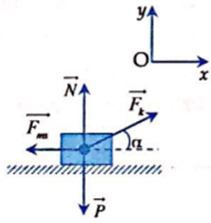
\includegraphics[scale=1]{../figs/VN10-2021-PH-TP024-4.png}
	\end{center}
	Chọn chiều dương trục $\text O x$ hướng theo phương chuyển động, trục $\text O y$ hướng theo phương trọng lực.
		
	Áp dụng định luật II Niu-tơn:
	$$\vec F + \vec P + \vec N + \vec F_\text{ms} = m \vec a$$
	
	Trên phương $\text Oy$:
	$$N = P - F \sin \alpha$$
	
	Trên phương $\text Ox$:
	$$F \cos \alpha - F_\text{ms} = ma \Rightarrow F \cos \alpha  - \mu (P-F \sin \alpha) = ma \Rightarrow a=\SI{0.83}{m/s^2}$$
	
	Vậy $s=\dfrac{1}{2}at^2 = \SI{6.65}{m}$.
	}
	
\end{enumerate}

\whiteBGstarEnd

\loigiai
{
	\begin{center}
		\textbf{BẢNG ĐÁP ÁN}
	\end{center}
	\begin{center}
		\begin{tabular}{|m{2.8em}|m{2.8em}|m{2.8em}|m{2.8em}|m{2.8em}|m{2.8em}|m{2.8em}|m{2.8em}|m{2.8em}|m{2.8em}|}
			\hline
			1.D  & 2.C  & 3.C  & 4.C  & 5.C  & & & & &  \\
			\hline
			
		\end{tabular}
	\end{center}
}
\section{Tự luận}
\begin{enumerate}[label=\bfseries Câu \arabic*:]
	\item \mkstar{1}
	
	\cauhoi{
	Momen lực có tác dụng như thế nào đối với một vật quay quanh một trục cố định? Mức quán tính của một vật quay quanh một trục phụ thuộc những yếu tố nào?
	}
	
	\loigiai{
		Momen lực tác dụng vào một vật quay quanh một trục cố định làm thay đổi tốc độ góc của vật.
		
		Mức quán tính của một vật quay quanh một trục phụ thuộc vào khối lượng của vật và sự phân bố khối lượng đó đối với trục quay.
	}
	
	\item \mkstar{2}
	
	\cauhoi
	{Có thể áp dụng định luật II Niu-tơn cho chuyển động tịnh tiến của một vật rắn được không? Tại sao?
	}
	
	\loigiai
	{
	Có thể áp dụng định luật II Niu-tơn cho chuyển động tịnh tiến của vật rắn. Vì tất cả các điểm của vật đều chuyển động với cùng một gia tốc, nên có thể xem vật rắn như một chất điểm.
	}
	\item \mkstar{3}
	
	\cauhoi
	{Một vật có khối lượng $m=\SI{40}{kg}$ bắt đầu trượt trên sàn nhà dưới tác dụng của một lực nằm ngang $F=\SI{200}{N}$. Hệ số ma sát trượt giữa vật và sàn là $\mu _\text t = \SI{0.25}{}$. Hãy tính:
		\begin{enumerate}
			\item Gia tốc của vật;
			\item Vận tốc của vật ở cuối giây thứ 3;
			\item Đoạn đường mà vật đi được trong 3 giây đầu.
		\end{enumerate}
	Lấy $g=\SI{10}{m/s^2}$.
	}
	
	\loigiai
	{		\begin{enumerate}
			\item Gia tốc của vật;
			
	Chọn hệ trục tọa độ $\text Oxy$ có O trùng với vị trí vật khi vật bắt đầu chuyển động. Chiều dương là chiều chuyển động.
	
	Áp dụng định luật II Niu-tơn:
	$$\vec P + \vec F + \vec N + \vec F_\text{ms} = m \vec a$$
	
	Chiếu lên $\text O x$:
	$$F-F_\text{ms} = ma$$
	
	Chiếu lên $\text O y$:
	$$N=P=mg$$
	
	Suy ra:
	$$F-\mu m g = ma \Rightarrow a = \SI{2.5}{m/s^2}$$
			\item Vận tốc của vật ở cuối giây thứ 3;
			
	$$v=at = \SI{7.5}{m/s}$$
	
			\item Đoạn đường mà vật đi được trong 3 giây đầu.
			
	$$s_3 = \dfrac{1}{2} at^2 = \SI{11.25}{m}$$
		\end{enumerate}
	}
	\item \mkstar{4}
	
	\cauhoi
	{Hai vật $m_1$ và $m_2$ được nối với nhau qua ròng rọc như hình vẽ.
		\begin{center}
			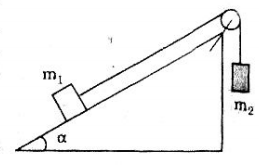
\includegraphics[scale=1]{../figs/VN10-2021-PH-TP024-1.png}
		\end{center}
	Hệ số ma sát giữa vật $m_1$ và mặt phẳng nghiêng là $\mu$. Bỏ qua khối lượng của ròng rọc và dây nối. Dây nối không giãn. Tính tỉ số $m_2 / m_1$ để vật $m_1$ đi lên thẳng đều.
	}
	
	\loigiai
	{		\begin{center}
			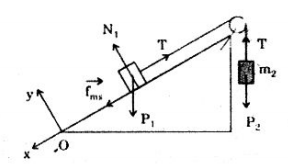
\includegraphics[scale=1.2]{../figs/VN10-2021-PH-TP024-2.png}
		\end{center}
		
		Vì vật chuyển động thẳng đều:
		$$\vec P_1 + \vec N_1 + T + \vec F_\text{ms} = 0$$
		
		Trên phương $\text Ox$:
		$$P_1 \sin \alpha - T + F_\text{ms} = 0 \Rightarrow P_2 \sin \alpha - P_2 + \mu N_1 = 0$$
		
		Trên phương $\text Oy$:
		$$N_1 = P_1 \cos \alpha$$
		
		Suy ra:
		$$P_1 \sin \alpha - P_2 + \mu P_1 \cos \alpha = 0 \Rightarrow P_1 (\sin \alpha + \mu \cos \alpha) = P_2 \Rightarrow \dfrac{P_2}{P_1} = \dfrac{m_2}{m_1} = \sin \alpha + \mu \cos \alpha$$
	}
	\item \mkstar{4}

\cauhoi
{Hai vật $m_1$ và $m_2$ được nối với nhau qua ròng rọc như hình vẽ.
	\begin{center}
		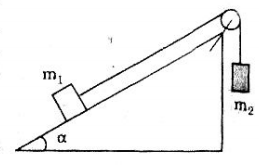
\includegraphics[scale=1]{../figs/VN10-2021-PH-TP024-1.png}
	\end{center}
	Hệ số ma sát giữa vật $m_1$ và mặt phẳng nghiêng là $\mu$. Bỏ qua khối lượng của ròng rọc và dây nối. Dây nối không giãn. Tính tỉ số $m_2 / m_1$ để vật $m_1$ đi xuống thẳng đều. Từ đố suy ra điều kiện $m_2 / m_1$ để vật $m_1$ đứng yên.
}

\loigiai
{		\begin{center}
		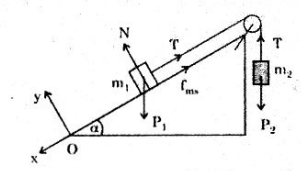
\includegraphics[scale=1.2]{../figs/VN10-2021-PH-TP024-3.png}
	\end{center}
	
	Lực ma sát hướng lên theo phương mặt phẳng nghiêng.
	
	Vì vật chuyển động thẳng đều:
	$$\vec P_1 + \vec N_1 + T + \vec F_\text{ms} = 0$$
	
	Trên phương $\text Ox$:
	$$P_1 \sin \alpha - T - F_\text{ms} = 0 \Rightarrow P_2 \sin \alpha - P_2 - \mu N_1 = 0$$
	
	Trên phương $\text Oy$:
	$$N_1 = P_1 \cos \alpha$$
	
	Suy ra:
	$$P_1 \sin \alpha - P_2 - \mu P_1 \cos \alpha = 0 \Rightarrow \dfrac{P_2}{P_1} = \dfrac{m_2}{m_1} = \sin \alpha - \mu \cos \alpha$$
	
	Dễ dàng suy luận được để $m_1$ đứng yên thì tỉ lệ $m_2 / m_1$ phải thỏa mãn điều kiện:
	$$\sin \alpha - \mu \cos \alpha \leq \dfrac{m_2}{m_1} \leq \sin \alpha + \mu \cos \alpha$$
}
\end{enumerate}
	\stopcontents[mychapters]
	
	\setcounter{mychapter}{24}
	\mychapter{Động năng}
	\startcontents[mychapters]
	\printcontents[mychapters]{}{0}{\setcounter{tocdepth}{1}}
	\whiteBGstarBegin
\setcounter{section}{0}
\section{Lý thuyết: Động năng}
\begin{enumerate}[label=\bfseries Câu \arabic*:]
		\item \mkstar{1} [5]
	
	\cauhoi{
		Động năng của một vật khối lượng $m$, chuyển động với vận tốc $v$ là
		\begin{mcq}(4)
			\item $W_\text{đ} = \dfrac{1}{2}mv$.
			\item $W_\text{đ} = \dfrac{1}{2}mv^2$.
			\item $W_\text{đ} = mv^2$.
			\item $W_\text{đ} = 2mv^2$.
		\end{mcq}
	}
	
	\loigiai{
		\textbf{Đáp án: B.}
		
		Động năng của một vật khối lượng $m$, chuyển động với vận tốc $v$ là $W_\text{đ} = \dfrac{1}{2}mv^2$.
	}
	
	\item \mkstar{1} [5]
	
	\cauhoi{
		Chọn phát biểu \textbf{sai}. Động năng của một vật không đổi khi vật chuyển động
		\begin{mcq}(2)
			\item tròn đều.
			\item với gia tốc không đổi.
			\item với vận tốc không đổi.
			\item thẳng đều.
		\end{mcq}
	}
	
	\loigiai{
		\textbf{Đáp án: B.}
		
		Khi vật chuyển động có gia tốc thì vận tốc thay đổi, do đó động năng thay đổi.
	}
	
	\item \mkstar{1} [24]
	
	\cauhoi{
		Động năng của vật tăng khi
		\begin{mcq}
			\item vận tốc của vật có giá trị âm.
			\item vận tốc của vật có giá trị dương.
			\item các lực tác dụng lên vật sinh công âm.
			\item các lực tác dụng lên vật sinh công dương.
		\end{mcq}
	}
	
	\loigiai{
		\textbf{Đáp án: D.}
		
		Các lực tác dụng lên vật sinh công dương thì $v$ tăng, do đó động năng tăng.
	}

	\item \mkstar{2} [5]
	
	\cauhoi{
		Một vật có khối lượng $\SI{0.5}{kg}$ chuyển động với vận tốc $\SI{10}{m/s}$. Động năng của vật bằng
		\begin{mcq}(4)
			\item $\SI{250}{J}$.
			\item $\SI{50}{J}$.
			\item $\SI{5}{J}$.
			\item $\SI{25}{J}$.
		\end{mcq}
	}
	
	\loigiai{
		\textbf{Đáp án: D.}
		
		Động năng của vật: $W_\text{đ} = \dfrac{1}{2}mv^2 = \SI{25}{J}$.
	}
	
	\item \mkstar{2} [5]
	
	\cauhoi{
		Một vận động viên có khối lượng $\SI{80}{kg}$ chạy đều hết quãng đường $\SI{180}{m}$ trong thời gian 40 giây. Động năng của vận động viên đó là
		\begin{mcq}(4)
			\item $\SI{810}{J}$. 
			\item $\SI{360}{J}$.
			\item $\SI{875}{J}$.
			\item $\SI{180}{J}$.
		\end{mcq}
		
	}
	
	\loigiai{
		\textbf{Đáp án: A.}
		
		Vận tốc của vận động viên:
		$$v=\dfrac{s}{t} = \SI{4.5}{m/s}.$$
		
		Động năng của vận động viên:
		$$W_\text{đ} = \dfrac{1}{2} mv^2 = \SI{810}{J}.$$
	}

	\item \mkstar{2} [24]
	
	\cauhoi{
		Khi vận tốc của vật tăng gấp đôi thì
		\begin{mcq}(2)
			\item động lượng của vật tăng gấp đôi.
			\item gia tốc của vật tăng gấp đôi.
			\item động năng của vật tăng gấp đôi.
			\item thế năng của vật tăng gấp đôi.
		\end{mcq}
	}
	
	\loigiai{
		\textbf{Đáp án: A.}
		
		Khi vận tốc của vật tăng gấp đôi thì động lượng của vật tăng gấp đôi, động năng của vật tăng gấp 4.
	}

	\item \mkstar{2} [24]
	
	\cauhoi{
		Một vật có khối lượng $\SI{250}{g}$ đang di chuyển với tốc độ $\SI{10}{m/s}$. Động năng của vật này là
		\begin{mcq}(4)
			\item $\SI{12.5}{J}$.
			\item $\SI{25}{J}$.
			\item $\SI{12500}{J}$.
			\item $\SI{25000}{J}$.
		\end{mcq}
	}
	
	\loigiai{
		\textbf{Đáp án: A.}
		
		Động năng của vật:
		$$W_\text{đ} = \dfrac{1}{2} mv^2  =\SI{12.5}{J}.$$
	}

	\item \mkstar{1} [7]
	
	\cauhoi{
		Động năng của một vật là gì? Nêu biểu thức tính động năng. Động năng là đại lượng vô hướng hay vectơ?
	}
	
	\loigiai{		
		Dạng năng lượng mà một vật có được do nó đang chuyển động gọi là động năng.
		
		Biểu thức tính động năng: $W_\text{đ} = \dfrac{1}{2}mv^2$.
		
		Động năng là đại lượng vô hướng.
	}
	
	
	\item \mkstar{2} [31]
	
	\cauhoi{
		Vật nặng $\SI{1}{kg}$ chuyển động với vận tốc $\SI{8}{m/s}$. Tính động năng của vật.
	}
	
	\loigiai{
		Động năng của vật:
		$$W_\text{đ} = \dfrac{1}{2}mv^2 = \SI{32}{J}.$$
	}

	
\end{enumerate}
\section{Lý thuyết: Biến thiên động năng}
\begin{enumerate}[label=\bfseries Câu \arabic*:]
	
	\item \mkstar{1} [4]
	
	\cauhoi{
		Độ biến thiên động năng của một vật chuyển động bằng
		\begin{mcq}
			\item công của lực ma sát tác dụng lên vật.
			\item công của lực thế (ví dụ: trọng lực) tác dụng lên vật.
			\item công của trọng lực tác dụng lên vật.
			\item công của các lực tác dụng lên vật.
		\end{mcq}
	}

\loigiai{
\textbf{Đáp án: D.}

Độ biến thiên động năng của một vật chuyển động bằng công của các lực tác dụng lên vật.
}

\item \mkstar{1} [20]

\cauhoi{
	Nêu mối liên hệ giữa công của lực tác dụng và độ biến thiên động năng (định lý động năng). Biểu thức của định lý.
}
\loigiai{
	
	Độ biến thiên động năng bằng công của các lực tác dụng vào vật.
	
	Biểu thức: $\dfrac{1}{2} mv^2 - \dfrac{1}{2}mv_0^2 = A$.
}

\item \mkstar{2} [9]

\cauhoi{
	Một ô tô khối lượng $m$ bằng 1 tấn đang chuyển động với vận tốc $v=\SI{20}{m/s}$. Tính độ biến thiên động năng của ô tô khi nó bị hãm tới khi vận tốc còn $\SI{10}{m/s}$.
}
\loigiai{
	
	Độ biến thiên động năng:
	$$\Delta W_\text{đ} = \dfrac{1}{2} m (v^2 - v_0^2) = \SI{-150000}{J}.$$
}

	\item \mkstar{3} [1]
	
	\cauhoi{
		Một xe khối lượng 1 tấn khởi hành không vận tốc đầu, chuyển động nhanh dần đều trên đường nằm ngang. Sau khi đi được quãng đường $\SI{100}{m}$ thì đạt vận tốc $\SI{72}{km/h}$. Biết lực ma sát bằng $5\%$ trọng lượng của xe. Dùng định lý động năng, tính công của lực kéo của động cơ xe.
	}
	\loigiai{
		
		Độ lớn lực ma sát bằng $5\%$ trong lượng xe nên $$F_\text{ms} = \dfrac{5mg}{100} = \SI{500}{N}.$$
		
		Áp dụng định lý động năng:
		$$A_F + A_\text{ms} = \dfrac{1}{2}mv^2 - 0 \Rightarrow A_F = \dfrac{1}{2} mv^2 - (-F_\text{ms}s) = \SI{250000}{J}.$$
	}

\item \mkstar{3} [3]

\cauhoi{
	Một vật nhỏ $m$ được truyền vận tốc đầu $v_0=\SI{5}{m/s}$ tại A để vật trượt trên mặt phẳng ngang $\text{AB} = \SI{3}{m}$. Hệ số ma sát giữa vật và mặt ngang là $\mu=\SI{0.2}{}$. Lấy $g=\SI{10}{m/s^2}$. Tính vận tốc $v$ của vật tại B.
}
\loigiai{
	
	Áp dụng định lý động năng:
	$$A_\text{ms} = \dfrac{1}{2}mv^2 - \dfrac{1}{2}mv_0^2 \Rightarrow -F_\text{ms}s = \dfrac{1}{2}mv^2 - \dfrac{1}{2}mv_0^2 \Rightarrow -\mu g s = \dfrac{1}{2}v^2 - \dfrac{1}{2}v_0^2 \Rightarrow v = \SI{3.6}{m/s}.$$
}



\item \mkstar{3} [13]

\cauhoi{
	Một ô tô có khối lượng 2 tấn đang chạy với vận tốc $\SI{54}{km/h}$ trên đường nằm ngang thì lái xe thấy có chướng ngại vật cách ô tô $\SI{100}{m}$ thì tắt máy, đạp thắng. Biết hệ số ma sát giữa bánh xe và mặt đường là $\mu = 0,1$. Xe ô tô có đâm vào chướng ngại vật không? Cho $g=\SI{10}{m/s^2}$.
}
\loigiai{
	
	Quãng đường xe chạy được cho đến khi dừng hẳn theo lý thuyết định lý động năng là
	$$-F_\text{ms}s = 0 - \dfrac{1}{2}mv^2 \Rightarrow s = \SI{112.5}{m}.$$
	
	Mà thực tế ô tô chỉ cách chướng ngại vật $\SI{100}{m}$, nên ô tô có đâm vào chướng ngại vật trước khi kịp dừng lại.
}

\item \mkstar{3} [25]

\cauhoi{
	Xe ô tô khối lượng 2 tấn bắt đầu khởi hành trên đường thẳng nằm ngang, đi được $\SI{50}{m}$ thì đạt được vận tốc $\SI{54}{km/h}$. Lực kéo của động cơ bằng $\SI{10000}{N}$. Lấy $g=\SI{10}{m/s^2}$.
	\begin{enumerate}[label=\alph*)]
		\item Dùng định lý động năng, tính công của lực ma sát.
		\item Tính độ lớn lực ma sát tác dụng lên xe trong đoạn đường trên.
	\end{enumerate}
}
\loigiai{
\begin{enumerate}[label=\alph*)]
	\item Dùng định lý động năng, tính công của lực ma sát.
	
	Áp dụng định lý động năng:
	$$A_F + A_\text{ms} = \dfrac{1}{2}mv^2 - 0 \Rightarrow A_\text{ms} = \dfrac{1}{2}mv^2 - A= \dfrac{1}{2} mv^2 - Fs= \SI{-275000}{J}.$$
	\item Tính độ lớn lực ma sát tác dụng lên xe trong đoạn đường trên.
	
	Ta có $A_\text{ms} = -F_\text{ms} s \Rightarrow F_\text{ms} = \SI{5500}{N}$.
\end{enumerate}
	
}

\item \mkstar{3} [25]

\cauhoi{
	Xe ô tô khối lượng 1 tấn bắt đầu khởi hành trên đường thẳng nằm ngang, đi được $\SI{50}{m}$ thì đạt được vận tốc $\SI{36}{km/h}$. Cho hệ số ma sát giữa bánh xe và mặt đường là $\SI{0.05}{}$. Lấy $g=\SI{10}{m/s^2}$. Dùng định lý động năng tính công của lực kéo của động cơ, từ đó suy ra độ lớn lực kéo của động cơ.
}
\loigiai{
	
	Áp dụng định lý động năng:
	$$A_F + A_\text{ms} = \dfrac{1}{2}mv^2 - 0 \Rightarrow A_F = \dfrac{1}{2}mv^2 - A_\text{ms} = \dfrac{1}{2}mv^2 - (-F_\text{ms}s) = \SI{75000}{J}.$$
	
	Lực kéo của động cơ:
	$$A_F=Fs \Rightarrow F = \SI{1500}{N}.$$
}

	\end{enumerate}
\whiteBGstarEnd
	\stopcontents[mychapters]
	
	\setcounter{mychapter}{25}
	\mychapter{Thế năng}
	\startcontents[mychapters]
	\printcontents[mychapters]{}{0}{\setcounter{tocdepth}{1}}
	\whiteBGstarBegin
\setcounter{section}{0}
\section{Lý thuyết: Thế năng trọng trường}
\begin{enumerate}[label=\bfseries Câu \arabic*:]
	
	\item \mkstar{1} [24]
	
	\cauhoi{
		Dạng năng lượng tương tác giữa Trái Đất và vật là
		\begin{mcq}(2)
			\item động năng.
			\item thế năng trọng trường.
			\item thế năng đàn hồi.
			\item cơ năng.
		\end{mcq}
	}
	
	\loigiai{
		\textbf{Đáp án: B.}
		
		Dạng năng lượng tương tác giữa Trái Đất và vật là thế năng trọng trường.
	}
	
	\item \mkstar{1} [32]
	
	\cauhoi{
		Thế năng trọng trường của một vật
		\begin{mcq}
			\item luôn dương vì độ cao của vật luôn dương. 
			\item có thể âm, dương hoặc bằng không.
			\item không thay đổi nếu vật chuyển động thẳng đều.
			\item không phụ thuộc vào vị trí của vật.
		\end{mcq}
		
	}
	
	\loigiai{
		\textbf{Đáp án: B.}
		
		Thế năng trọng trường của một vật có thể âm, dương hoặc bằng không.
	}

	
	\item \mkstar{1} [7]
	
	\cauhoi{
		Viết biểu thức thế năng trọng trường của vật (có chú thích các đại lượng trong công thức). Chọn gốc thế năng tại mặt đất, khi thả một vật rơi tự do thì thế năng trọng trường của vật tăng hay giảm? (không cần giải thích)
	}
	
	\loigiai{		
		Biểu thức thế năng trọng trường:
		$$W_\text t = mgh,$$
		với:
		\begin{itemize}
			\item $m$ là khối lượng của vật (đơn vị kg);
			\item $g$ là gia tốc trọng trường nơi đặt vật (đơn vị $\SI{}{m/s^2}$);
			\item $h$ là vị trí của vật so với gốc thế năng (đơn vị $\SI{}{m}$).
		\end{itemize}
	
		Chọn gốc thế năng tại mặt đất, khi thả một vật rơi tự do thì thế năng trọng trường của vật giảm.
	}
	
	
	\item \mkstar{2} [13]
	
	\cauhoi{
		Một vật có khối lượng $\SI{2}{kg}$ được thả rơi từ độ cao $\SI{4.5}{m}$ xuống mặt đất, tại nơi có gia tốc trọng trường là $\SI{10}{m/s^2}$. Xác định thế năng của vật.
	}
	
	\loigiai{
		Chọn gốc thế năng tại mặt đất. Thế năng của vật:
		$$W_\text t = mgz = \SI{90}{J}.$$
	}
	
	\item \mkstar{2} [15]
	
	\cauhoi{
		Dùng lực để nâng vật có khối lượng $\SI{180}{g}$ thẳng đứng lên cao một đoạn $\SI{50}{cm}$. Tìm công của trọng lực trong quá trình trên. Lấy $g=\SI{10}{m/s^2}$.
	}
	
	\loigiai{
		Công của trọng lực:
		$$A_P = mgh\cos(180^\circ) = -mgh = \SI{-0.9}{J}.$$
		
	}
\end{enumerate}
\section{Lý thuyết: Thế năng đàn hồi}
\begin{enumerate}[label=\bfseries Câu \arabic*:]
		
	\item \mkstar{1} [29]
	
	\cauhoi{
		Một con lắc lò xo có độ cứng $k$, lò xo bị nén một đoạn $\Delta l$, biểu thức tính thế năng đàn hồi của lò xo là
		\begin{mcq}(4)
			\item $W_\text t =k(\Delta l)^2$. 
			\item $W_\text t = k |\Delta l|$.
			\item $W_\text t = \dfrac{1}{2}k (\Delta l)^2$.
			\item $W_\text t = \dfrac{1}{2} k |\Delta l|$.
		\end{mcq}
		
	}
	
	\loigiai{
		\textbf{Đáp án: C.}
		
		Một con lắc lò xo có độ cứng $k$, lò xo bị nén một đoạn $\Delta l$, biểu thức tính thế năng đàn hồi của lò xo là $W_\text t = \dfrac{1}{2}k (\Delta l)^2$.
	}


	\item \mkstar{2} [8]
	
	\cauhoi{
		Một lò xo nằm ngang ở trạng thái ban đầu không biến dạng có độ cứng là $\SI{100}{N/m}$. Tính thế năng đàn hồi của lò xo khi nó bị giãn ra $\SI{4}{cm}$.
		
	}
	
	\loigiai{
		Thế năng đàn hồi của lò xo:
		$$W_\text t = \dfrac{1}{2} k (\Delta l)^2 = \SI{0.08}{J}.$$
	}

	
\end{enumerate}	
\whiteBGstarEnd
	\stopcontents[mychapters]
	
	\setcounter{mychapter}{26}
	\mychapter{Cơ năng}
	\startcontents[mychapters]
	\printcontents[mychapters]{}{0}{\setcounter{tocdepth}{1}}
	\whiteBGstarBegin
\setcounter{section}{0}
\section{Lý thuyết: Cơ năng của vật chuyển động trong trọng trường}
\begin{enumerate}[label=\bfseries Câu \arabic*:]
	\item \mkstar{1} [29]
	
	\cauhoi{
		Trong quá trình chuyển động, nếu vật chỉ chịu tác dụng của trọng lực thì cơ năng của vật đó được tính bởi hệ thức
		\begin{mcq}(2)
			\item $W=2mgz+mv^2$.
			\item $W=mgz+mv^2$.
			\item $W=2mgz+\dfrac{1}{2}mv^2$.
			\item $W=mgz+\dfrac{1}{2}mv^2$.
		\end{mcq}
	}
	
	\loigiai{
		\textbf{Đáp án: D.}
		
		Cơ năng của vật bằng tổng động năng và thế năng:
		$$W=mgz+\dfrac{1}{2}mv^2.$$
	}
	
	\item \mkstar{2} [5]
	
	\cauhoi{
		Một vật có khối lượng $\SI{2}{kg}$ rơi tự do không vận tốc đầu từ độ cao $\SI{5}{m}$ xuống mặt đất. Lấy $g=\SI{10}{m/s^2}$. Cơ năng của vật bằng
		\begin{mcq}(4)
			\item $\SI{10}{J}$.
			\item $\SI{100}{J}$.
			\item $\SI{50}{J}$.
			\item $\SI{5}{J}$.
		\end{mcq}
	}
	
	\loigiai{
		\textbf{Đáp án: B.}
		
		Cơ năng của vật bằng tổng động năng và thế năng (vì $v=0$ nên động năng bằng 0):
		$$W=W_\text t = mgh = \SI{100}{J}.$$
	}
	
	\item \mkstar{2} [5]
	
	\cauhoi{
		Từ điểm M có độ cao $\SI{0.8}{m}$ so với mặt đất, người ta ném lên một vật có khối lượng $\SI{0.5}{kg}$ với vận tốc $\SI{2}{m/s}$. Lấy $g=\SI{10}{m/s^2}$. Cơ năng của vật bằng
		\begin{mcq}(4)
			\item $\SI{5}{J}$. 
			\item $\SI{8}{J}$.
			\item $\SI{4}{J}$.
			\item $\SI{1}{J}$.
		\end{mcq}
		
	}
	
	\loigiai{
		\textbf{Đáp án: A.}
		
		Cơ năng của vật bằng tổng động năng và thế năng:
		$$W=mgh + \dfrac{1}{2}mv^2 = \SI{5}{J}.$$
	}
	
	\item \mkstar{2} [24]
	
	\cauhoi{
		Một vật có khối lượng $m=\SI{1}{kg}$ được thả rơi tự do từ độ cao $\SI{20}{m}$ so với mặt đất. Chọn gốc thế năng tại mặt đất. Bỏ qua mọi ma sát. Ngay khi vật chạm đất thì
		\begin{mcq}
			\item động năng cực đại, thế năng cực tiểu.
			\item động năng bằng thế năng.
			\item động năng cực tiểu, thế năng cực đại.
			\item động năng bằng một nửa thế năng.
		\end{mcq}
	}
	
	\loigiai{
		\textbf{Đáp án: A.}
		
		Khi vật chạm đất thì động năng cực đại vì $v$ cực đại, thế năng cực tiểu vì $h$ cực tiểu.
	}
	
	\item \mkstar{2} [24]
	
	\cauhoi{
		Một vật có khối lượng $\SI{100}{g}$ được ném thẳng đứng lên cao với vận tốc $\SI{10}{m/s}$ từ độ cao $\SI{5}{m}$ so với mặt đất. Chọn gốc thế năng tại mặt đất. Lấy $g=\SI{10}{m/s^2}$. Cơ năng của vật khi chuyển động là
		\begin{mcq}(4)
			\item $\SI{15}{J}$.
			\item $\SI{11.25}{J}$.
			\item $\SI{10.5}{J}$.
			\item $\SI{10}{J}$.
		\end{mcq}
	}
	
	\loigiai{
		\textbf{Đáp án: D.}
		
		Cơ năng của vật bằng tổng động năng và thế năng:
		$$W=mgh + \dfrac{1}{2}mv^2 = \SI{10}{J}.$$
	}
	
	\item \mkstar{1} [22]
	
	\cauhoi{
		Định nghĩa và viết công thức cơ năng của vật chuyển động trong trọng trường.
	}
	
	\loigiai{
		Cơ năng của vật chuyển động dưới tác dụng của trọng lực bằng tổng động năng và thế năng trọng trường của vật.
		$$W=W_\text{đ}+W_\text{t}=\dfrac{mv^2}{2} + mgz.$$
		
	}
	
	\item \mkstar{2} [17]
	
	\cauhoi{
		Từ điểm A cách mặt đất $\SI{1}{m}$, một vật có khối lượng $\SI{0.5}{kg}$ được ném thẳng đứng lên trên với vận tốc $\SI{4}{m/s}$. Lấy $g=\SI{10}{m/s^2}$. Bỏ qua sức cản của không khí. Chọn gốc thế năng tại mặt đất. Tính cơ năng của vật tại vị trí ném.
	}
	
	\loigiai{		
		Cơ năng của vật bằng tổng động năng và thế năng:
		$$W=mgz+\dfrac{1}{2}mv^2 = \SI{9}{J}.$$
	}
	
	
	\item \mkstar{2} [20]
	
	\cauhoi{
		Người ta ném một quả bóng có khối lượng $m=\SI{200}{g}$ từ độ cao $\SI{2}{m}$ so với mặt đất lên cao với vận tốc $\SI{5}{m/s}$. Cho $g=\SI{10}{m/s^2}$. Chọn gốc thế năng tại mặt đất. Tính động năng, thế năng, cơ năng của quả bóng tại vị trí ném.
	}
	
	\loigiai{
		Động năng:
		$$W_\text{đ} = \dfrac{1}{2}mv^2 = \SI{2.5}{J}.$$
		
		Thế năng:
		$$W_\text t = mgz = \SI{4}{J}.$$
		
		Cơ năng:
		$$W=W_\text{đ} + W_\text t = \SI{6.5}{J}.$$
	}
	
	\item \mkstar{3} [21]
	
	\cauhoi{
		Ném thẳng đứng xuống dưới một vật khối lượng $\SI{200}{g}$ với vận tốc $\SI{5}{m/s}$ từ độ cao $\SI{1.5}{m}$ so với mặt đất. Bỏ qua mọi lực cản. Cho $g=\SI{10}{m/s^2}$. Tính động năng, thế năng và cơ năng của vật
		\begin{enumerate}[label=\alph*)]
			\item ngay lúc ném.
			\item ngay trước khi chạm đất.
		\end{enumerate}
	}
	
	\loigiai{
		\begin{enumerate}[label=\alph*)]
			\item Tính động năng, thế năng và cơ năng của vật ngay lúc ném.
			
			Động năng:
			$$W_\text{đ 1} = \dfrac{1}{2}mv_1^2 = \SI{2.5}{J}.$$
			
			Thế năng:
			$$W_\text{t 1} = mgz_1 = \SI{3}{J}.$$
			
			Cơ năng:
			$$W_1 = W_\text{đ 1} + W_\text{t 1} = \SI{5.5}{J}.$$
			\item Tính động năng, thế năng và cơ năng của vật ngay trước khi chạm đất.
			
			Khi chạm đất thì $z_2 = 0$, suy ra $W_\text{t 2} = 0$.
			
			Khi đó cơ năng bằng động năng và bằng cơ năng ban đầu:
			$$W_2 = W_\text{đ 2} = W_1 = \SI{5.5}{J}.$$
		\end{enumerate}
		
	}
	
\end{enumerate}
\section{Lý thuyết: Bảo toàn cơ năng của vật chuyển động trong trọng trường}
\begin{enumerate}[label=\bfseries Câu \arabic*:]
	\item \mkstar{1} [32]
	
	\cauhoi{
		Khi một vật chuyển động trong trọng trường chỉ chịu tác dụng của trọng lực thì
		\begin{mcq}
			\item cơ năng của vật là một đại lượng bảo toàn.
			\item động lượng của vật là một đại lượng bảo toàn.
			\item thế năng của vật là một đại lượng bảo toàn.
			\item động năng của vật là một đại lượng bảo toàn.
		\end{mcq}
	}
	
	\loigiai{
		\textbf{Đáp án: A.}
		
		Khi một vật chuyển động trong trọng trường chỉ chịu tác dụng của trọng lực thì cơ năng của vật là một đại lượng bảo toàn.
	}
	
	\item \mkstar{1} [32]
	
	\cauhoi{
		Một vật nhỏ được ném thẳng đứng hướng xuống từ một điểm phía trên mặt đất. Bỏ qua sức cản của không khí. Trong quá trình vật rơi thì
		\begin{mcq}
			\item động năng và thế năng của vật tăng.
			\item động năng và thế năng của vật giảm.
			\item động năng tăng, thế năng giảm.
			\item động năng hoặc thế năng bảo toàn.
		\end{mcq}
	}
	
	\loigiai{
		\textbf{Đáp án: C.}
		
		Trong quá trình vật rơi thì động năng tăng vì $v$ tăng, thế năng giảm vì $z$ giảm.
	}
	
	\item \mkstar{2} [27]
	
	\cauhoi{
		Một vật khối lượng $m=\SI{2}{kg}$ được ném theo phương thẳng đứng hướng xuống từ độ cao $\SI{15}{m}$ so với mặt đất với tốc độ $\SI{10}{m/s}$. Bỏ qua mọi lực cản. Chọn gốc thế năng tại mặt đất. Lấy $g=\SI{10}{m/s^2}$. Tốc độ của vật khi vật vừa chạm đất là
		\begin{mcq}(4)
			\item $\SI{10}{m/s}$.
			\item $\SI{15}{m/s}$.
			\item $\SI{20}{m/s}$.
			\item $\SI{400}{m/s}$.
		\end{mcq}
	}
	
	\loigiai{
		\textbf{Đáp án: C.}
		
		Bảo toàn cơ năng lúc vừa ném và lúc vừa chạm đất:
		$$W_1 = W_2 \Rightarrow W_\text{đ 1} + W_\text{t 1} = W_\text{đ 2} + W_\text{t 2} \Rightarrow \dfrac{1}{2}mv_1^2 + mgz_1 = \dfrac{1}{2}mv_2^2 + mgz_2.$$
		$$\Rightarrow \dfrac{1}{2}v_1^2 + gz_1 = \dfrac{1}{2}v_2^2 + gz_2 \Rightarrow v_2 = \SI{20}{m/s}.$$
	}
	
	\item \mkstar{1} [9]
	
	\cauhoi{
		Phát biểu và viết biểu thức của định luật bảo toàn cơ năng của vật chuyển động trong trọng trường.
		
	}
	\loigiai{
		
		Khi một vật chuyển động trong trọng trường và chỉ chịu tác dụng của trọng lực thì cơ năng của vật được bảo toàn.
		
		Biểu thức: $W=W_\text{đ} + W_\text{t} = \dfrac{1}{2}mv^2 + mgz = \text{hằng số}$, trong đó:
		\begin{itemize}
			\item $m$ là khối lượng (đơn vị $\SI{}{kg}$);
			\item $g$ là gia tốc trọng trường (đơn vị $\SI{}{m/s^2}$);
			\item $z$ là vị trí của vật so với gốc thế năng (đơn vị $\SI{}{m}$);
			\item $v$ là vận tốc của vật (đơn vị $\SI{}{m/s}$).
		\end{itemize}
	}
	
	\item \mkstar{2} [6]
	
	\cauhoi{
		Một vật khối lượng $\SI{2}{kg}$ được ném thẳng đứng với vận tốc ban đầu $\SI{20}{m/s}$ xuống đất. Lấy $g=\SI{10}{m/s^2}$. Chọn gốc thế năng tại mặt đất. Bỏ qua lực cản của không khí trong quá trình vật chuyển động.
		\begin{enumerate}[label=\alph*)]
			\item Tính cơ năng của vật lúc ném.
			\item Tìm vận tốc của vật khi chạm đất.
		\end{enumerate}
		
	}
	\loigiai{
		
		\begin{enumerate}[label=\alph*)]
			\item Tính cơ năng của vật lúc ném.
			
			Cơ năng:
			$$W_1 = W_\text{đ 1} + W_\text{t 1} = \SI{400}{J}.$$
			\item Tìm vận tốc của vật khi chạm đất.
			
			Áp dụng bảo toàn cơ năng:
			$$W_1 = W_2 \Rightarrow \SI{400}{J} = \dfrac{1}{2}mv_2^2 + 0 \Rightarrow v_2 = \SI{20}{m/s}.$$
		\end{enumerate}
	}
	
	\item \mkstar{2} [9]
	
	\cauhoi{
		Vật có khối lượng $m=\SI{2}{kg}$ được thả rơi tự do từ độ cao $\SI{40}{m}$ so với mặt đất. Cho $g=\SI{10}{m/s^2}$. Chọn gốc thế năng tại mặt đất.
		\begin{enumerate}[label=\alph*)]
			\item Tính động năng của vật lúc chạm đất.
			\item Ở độ cao nào vật có động năng bằng thế năng?
		\end{enumerate}
		
	}
	\loigiai{
		
		\begin{enumerate}[label=\alph*)]
			\item Tính động năng của vật lúc chạm đất.
			
			Áp dụng bảo toàn cơ năng cho lúc thả vật và lúc chạm đất:
			$$W_1 = W_2 \Rightarrow mgz_1 + 0 = W_\text{đ 2} + 0 \Rightarrow W_\text{đ 2} = \SI{800}{J}.$$
			
			\item Ở độ cao nào vật có động năng bằng thế năng?
			
			Áp dụng bảo toàn cơ năng:
			$$W_1 = W_3 \Rightarrow W_1 = W_\text{đ 3} + W_\text{t 3} \Rightarrow W_1 = 2 W_\text{t 3} \Rightarrow \SI{800}{J} = 2 mgz_3 \Rightarrow z_3 = \SI{20}{m}.$$
		\end{enumerate}
	}
	
	\item \mkstar{2} [11]
	
	\cauhoi{
		Ném vật khối lượng $\SI{150}{g}$ thẳng đứng lên cao từ mặt đất với vận tốc $\SI{20}{m/s}$. Bỏ qua sức cản không khí. Cho $g=\SI{10}{m/s^2}$. Chọn gốc thế năng tại mặt đất.
		\begin{enumerate}[label=\alph*)]
			\item Tính động năng, cơ năng của vật tại vị trí ném.
			\item Tìm độ cao cực đại mà vật đạt được.
		\end{enumerate}
		
	}
	\loigiai{
		
		\begin{enumerate}[label=\alph*)]
			\item Tính động năng, cơ năng của vật tại vị trí ném.
			
			Động năng:
			$$W_\text{đ 1} = \dfrac{1}{2}mv_1^2 = \SI{30}{J}.$$
			
			Cơ năng:
			$$W_1 = W_\text{đ 1} + 0 = \SI{30}{J}.$$
			\item Tìm độ cao cực đại mà vật đạt được.
			
			Độ cao cực đại mà vật đạt được:
			$$W_1 = W_3 \Rightarrow \SI{30}{J} = 0 + mgz_3 \Rightarrow z_3 = \SI{20}{m}.$$
		\end{enumerate}
		
	}
	
	\item \mkstar{2} [14]
	
	\cauhoi{
		Một vật có khối lượng $\SI{2}{kg}$ được thả rơi tự do từ độ cao $\SI{2.5}{m}$ so với mặt đất. Lấy $g=\SI{10}{m/s^2}$, bỏ qua mọi lực cản của không khí. Chọn gốc thế năng ở mặt đất. Xác định vận tốc của vật khi đạt đến vị trí có độ cao giảm đi một nửa.
		
	}
	\loigiai{
		
		Tại vị trí có độ cao giảm đi một nửa thì $z_2=\dfrac{z_2}{2} = \SI{1.25}{m}$. Áp dụng bảo toàn cơ năng:
		
		$$W_1 = W_2 \Rightarrow 0 + mgz_1 = \dfrac{1}{2}mv_2^2 + mgz_2 \Rightarrow v_2 = \SI{5}{m/s}.$$
	}
	
	\item \mkstar{2} [15]
	
	\cauhoi{
		Một viên bi được ném từ mặt đất thẳng đứng lên cao với vận tốc ban đầu $\SI{10}{m/s}$. Bỏ qua lực cản không khí, chọn gốc thế năng tại mặt đất, lấy $g=\SI{10}{m/s^2}$. Dùng phương pháp bảo toàn năng lượng, hãy tìm độ cao cực đại mà viên bi lên được.
		
	}
	\loigiai{
		Áp dụng bảo toàn cơ năng:
		
		$$W_1 = W_2 \Rightarrow \dfrac{1}{2}mv_1^2 + 0 = 0 + mgz_2 \Rightarrow z_2 = \SI{5}{m}.$$
	}
	
	\item \mkstar{2} [15]
	
	\cauhoi{
		Một viên bi được thả rơi tự do từ độ cao $\SI{5}{m}$ so với mặt đất, chọn gốc thế năng tại mặt đất và lấy $g=\SI{10}{m/s^2}$. Dùng phương pháp năng lượng, hãy tìm vận tốc của viên bi khi chạm đất.
		
	}
	\loigiai{
		
		Áp dụng bảo toàn cơ năng:
		
		$$W_1 = W_2 \Rightarrow 0 + mgz_1 = \dfrac{1}{2}mv_2^2 + 0 \Rightarrow v_2 = \SI{10}{m/s}.$$
	}
	
	\item \mkstar{2} [21]
	
	\cauhoi{
		Ném thẳng đứng xuống dưới một vật khối lượng $\SI{200}{g}$ với vận tốc $\SI{5}{m/s}$ từ độ cao $\SI{1.5}{m}$ so với mặt đất. Bỏ qua mọi lực cản, cho $g=\SI{10}{m/s^2}$. Tính động năng, thế năng và cơ năng của vật tại
		\begin{enumerate}[label=\alph*)]
			\item lúc ném.
			\item lúc vật chạm đất.
		\end{enumerate}
		
	}
	\loigiai{
		
		\begin{enumerate}[label=\alph*)]
			\item Tính động năng, thế năng và cơ năng của vật tại lúc ném.
			
			Động năng:
			$$W_\text{đ 1} = \dfrac{1}{2}mv_1^2 = \SI{2.5}{J}.$$
			
			Thế năng:
			$$W_\text{t 1} = mgz_1 = \SI{3}{J}.$$
			
			Cơ năng:
			$$W_1 = W_\text{đ 1} + W_\text{t 1} = \SI{5.5}{J}.$$
			\item Tính động năng, thế năng và cơ năng của vật tại lúc vật chạm đất.
			
			Khi vật chạm đất, thế năng $W_\text{t 2} = 0$, động năng bằng cơ năng:
			$$W_\text{đ 2}  =W_2 = W_1 = \SI{5.5}{J}.$$
		\end{enumerate}
	}
	
	\item \mkstar{2} [30]
	
	\cauhoi{
		Một người trượt trên máng cong như hình bên. Nếu bỏ qua ma sát trong quá trình chuyển động thì cơ năng trong trường hợp này có được bảo toàn không? Vì sao?
		\begin{center}
			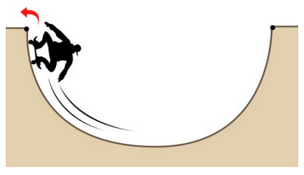
\includegraphics[scale=0.9]{../figs/VN10-2021-PH-TP027-3}
		\end{center}
		
	}
	\loigiai{
		
		Nếu bỏ qua ma sát thì người trượt ván chỉ chịu tác dụng của trọng lực, do đó cơ năng được bảo toàn.
	}
	
	\item \mkstar{2} [31]
	
	\cauhoi{
		Một vật trượt không vận tốc đầu từ đỉnh một mặt phẳng nghiêng cao $\SI{1.25}{m}$. Cho gia tốc rơi tự do $g=\SI{10}{m/s^2}$. Vật trượt không ma sát trên mặt phẳng nghiêng. Hãy tính vận tốc của vật tại chân mặt phẳng nghiêng.
	}
	
	\loigiai{
		
		Chọn gốc thế năng tại chân mặt phẳng nghiêng. Áp dụng bảo toàn cơ năng:
		$$W_1 = W_2 \Rightarrow 0 + mgz_1 = \dfrac{1}{2}mv_2^2 + 0 \Rightarrow v_2 = \SI{5}{m/s}.$$
	}
	
	\item \mkstar{3} [4]
	
	\cauhoi{
		Một vật khối lượng $\SI{1}{kg}$ được ném từ mặt đất lên cao theo phương thẳng đứng với vận tốc ban đầu là $\SI{10}{m/s}$. Bỏ qua mọi lực cản của môi trường và lấy $g=\SI{10}{m/s^2}$
		\begin{enumerate}[label=\alph*)]
			\item Tính cơ năng ban đầu.
			\item Khi vật lên đến độ cao bằng $2/3$ độ cao cực đại so với nơi ném thì vật có vận tốc bằng bao nhiêu?
		\end{enumerate}
	}
	\loigiai{
		
		\begin{enumerate}[label=\alph*)]
			\item Tính cơ năng ban đầu.
			
			Cơ năng vật tại nơi ném:
			$$W_1=W_\text{đ} + W_\text{t} = \dfrac{1}{2}mv_1^2 + 0 = \SI{50}{J}.$$
			\item Khi vật lên đến độ cao bằng $2/3$ độ cao cực đại so với nơi ném thì vật có vận tốc bằng bao nhiêu?
			
			Bảo toàn cơ năng tại vị trí ném và tại vị trí vật có độ cao cực đại:
			$$W_1 = W_2 \Rightarrow \SI{50}{J} = 0 + mgz_2 \Rightarrow z_2 = \SI{5}{m}.$$
			
			Bảo toàn cơ năng tại vị trí ném và tại vị trí vật có độ cao bằng $2/3$ độ cao cực đại ($z_3=\SI{3.33}{m}$):
			$$W_1 = W_3 \Rightarrow \SI{50}{J} = \dfrac{1}{2}mv_3^2 + mgz_3 \Rightarrow v_3 \approx \SI{5.77}{m/s}.$$
		\end{enumerate}
	}
	
	\item \mkstar{3} [8]
	
	\cauhoi{
		Một vật có khối lượng $\SI{1}{kg}$ được thả rơi không vận tốc đầu từ độ cao $\SI{20}{m}$ so với mặt đất. Bỏ qua lực cản của không khí. Chọn gốc thế năng tại mặt đất, lấy $g=\SI{10}{m/s^2}$.
		\begin{enumerate}[label=\alph*)]
			\item Tính cơ năng của vật tại điểm thả.
			\item Tính độ cao khi vật đạt vận tốc $\SI{36}{km/h}$.
			\item Tính vận tốc cực đại của vật.
		\end{enumerate}
		
	}
	\loigiai{
		
		\begin{enumerate}[label=\alph*)]
			\item Tính cơ năng của vật tại điểm thả.
			
			Cơ năng:
			$$W_1 = W_\text{đ 1} + W_\text{t 1} = 0 + mgz_1 = \SI{200}{J}.$$
			
			\item Tính độ cao khi vật đạt vận tốc $\SI{36}{km/h}$.
			
			Áp dụng bảo toàn cơ năng với $v_2 = \SI{10}{m/s}$:
			
			$$W_1 = W_2 \Rightarrow \SI{200}{J} = \dfrac{1}{2}mv_2^2 + mgz_2 \Rightarrow z_2 = \SI{15}{m}.$$
			
			\item Tính vận tốc cực đại của vật.
			
			Khi $v_3$ cực đại thì $z_3 = 0$, khi đó vật ở mặt đất. Áp dụng bảo toàn cơ năng:
			$$W_1 = W_3 \Rightarrow \SI{200}{J} = \dfrac{1}{2}mv_3^2 + 0 \Rightarrow v_3 = \SI{20}{m/s}.$$
		\end{enumerate}
	}
	
	
	\item \mkstar{3} [10]
	
	\cauhoi{
		\begin{minipage}[l]{0.7\textwidth}
			Trượt từ cầu trượt xuống nước là một trò chơi cảm giác mạnh được các bạn trẻ rất yêu thích trong công viên nước Đầm Sen vào những ngày hè nóng bức. Một học sinh có khối lượng $\SI{50}{kg}$ bắt đầu trượt không vận tốc đầu từ đỉnh cầu trượt ba chiều từ độ cao $h=\SI{10}{m}$ so với mặt nước. Giả thiết cầu trượt không ma sát, lấy $g=\SI{10}{m/s^2}$.
			\begin{enumerate}[label=\alph*)]
				\item Tính vận tốc của bạn học sinh khi vừa chạm mặt nước.
				\item Ở độ cao nào bạn học sinh có động năng bằng 2 lần thế năng?
			\end{enumerate}
		\end{minipage}
		\begin{minipage}[r]{0.3\textwidth}
			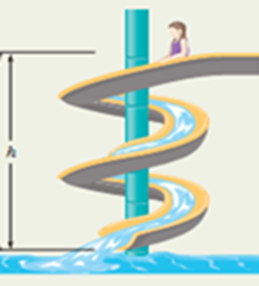
\includegraphics{../figs/VN10-2021-PH-TP027-1.png}
		\end{minipage}
	}
	\loigiai{
		
		\begin{enumerate}[label=\alph*)]
			\item Tính vận tốc của bạn học sinh khi vừa chạm mặt nước.
			
			Chọn gốc thế năng tại mặt nước. Áp dụng bảo toàn cơ năng:
			$$W_1 = W_2 \Rightarrow 0 + mgz_1 = \dfrac{1}{2}mv_2^2 + 0 \Rightarrow v_2 = \xsi{10\sqrt 2}{m/s}.$$
			\item Ở độ cao nào bạn học sinh có động năng bằng 2 lần thế năng?
			
			Áp dụng bảo toàn cơ năng với $W_\text{đ 3} = 2 W_\text{t 3}$:
			$$W_1 = W_3 \Rightarrow W_1 = 2W_\text{t 3} + W_\text{t 3} = 3 mgz_3 \Rightarrow z_3 = \xsi{10/3}{m}.$$
		\end{enumerate}
	}
	
	\item \mkstar{3} [12]
	
	\cauhoi{
		Một viên bi nhỏ khối lượng $\SI{200}{g}$ được ném thẳng đứng xuống dưới từ điểm O có độ cao $\SI{7}{m}$ so với mặt đất với tốc độ ban đầu $\SI{4}{m/s}$. Bỏ qua sức cản của không khí, lấy $g=\SI{10}{m/s^2}$. Giải bài toán bằng phương pháp năng lượng, chọn gốc thế năng tại mặt đất.
		\begin{enumerate}[label=\alph*)]
			\item Tìm độ cao của điểm M mà tại đó thế năng và động năng của viên bi bằng nhau.
			\item Tính tốc độ của viên bi ngay trước lúc chạm đất tại A.
		\end{enumerate}
		
	}
	\loigiai{
		
		\begin{enumerate}[label=\alph*)]
			\item Tìm độ cao của điểm M mà tại đó thế năng và động năng của viên bi bằng nhau.
			
			Khi $W_\text{đ M} = W_\text{t M}$ thì $\dfrac{1}{2}mv_\text{M}^2 = mgz_\text{M}$, áp dụng bảo toàn cơ năng tại O và M:
			$$W_\text{O} = W_\text{M} \Rightarrow \dfrac{1}{2}mv_\text{O}^2 + mgz_\text{O} = 2mgz_\text{M} \Rightarrow z_\text{M} = \SI{3.9}{m}.$$
			\item Tính tốc độ của viên bi ngay trước lúc chạm đất tại A.
			
			Áp dụng bảo toàn cơ năng tại O và A, với $z_\text{A} = 0$:
			$$W_\text{O} = W_\text{A} \Rightarrow \dfrac{1}{2}mv_\text{O}^2 + mgz_\text{O} = \dfrac{1}{2}mv_\text{A}^2 \Rightarrow v_\text{A} = \xsi{\sqrt{156}}{m/s}.$$
		\end{enumerate}
	}
	
	\item \mkstar{3} [13]
	
	\cauhoi{
		Từ độ cao $\SI{10}{m}$ người ta thả rơi một vật khối lượng $\SI{2}{kg}$. Bỏ qua lực cản không khí, lấy $g=\SI{10}{m/s^2}$. Tính tốc độ của vật khi động năng của nó lớn hơn thế năng $\SI{60}{J}$.
		
	}
	\loigiai{
		
		Chọn gốc thế năng tại mặt đất. Gọi A, B lần lượt là vị trí thả vật và vị trí có động năng lớn hơn thế năng $\SI{60}{J}$. 
		
		Ta có $W_\text{đ B} = W_\text{t B} + 60 \Rightarrow W_\text{t B} = W_\text{đ B} - 60$.
		
		Áp dụng bảo toàn cơ năng tại A và B:
		$$W_\text{A} = W_\text{B} \Rightarrow 0 + mgz_\text{A} = W_\text{đ B} + (W_\text{đ B} - 60) = 2 W_\text{đ B} - 60 \Rightarrow v_\text{B} = \xsi{\sqrt{130}}{m/s}.$$
	}
	
	\item \mkstar{3} [18]
	
	\cauhoi{
		Một vật có khối lượng $\SI{2}{kg}$ rơi tự do từ độ cao $h=\SI{100}{cm}$ xuống đất. Chọn gốc thế năng tại mặt đất, lấy $g=\SI{10}{m/s^2}$.
		\begin{enumerate}[label=\alph*)]
			\item Tính vận tốc cực đại trong quá trình chuyển động của vật.
			\item Khi động năng bằng 2 lần thế năng thì vật ở độ cao bao nhiêu?
		\end{enumerate}
	}
	\loigiai{
		
		\begin{enumerate}[label=\alph*)]
			\item Tính vận tốc cực đại trong quá trình chuyển động của vật.
			
			Vận tốc vật cực đại khi $z_2 = 0$, áp dụng bảo toàn cơ năng:
			$$W_1 = W_2 \Rightarrow 0 + mgz_1 = \dfrac{1}{2}mv_2^2 + 0 \Rightarrow v_2 = \xsi{2\sqrt5}{m/s}.$$
			\item Khi động năng bằng 2 lần thế năng thì vật ở độ cao bao nhiêu?
			
			Khi $W_\text{đ 3} = 2 W_\text{t 3}$ thì $W_3 = 3_\text{t 3}$. Áp dụng bảo toàn cơ năng:
			$$W_1 = W_3 \Rightarrow 0 + mgz_1 = 3 mgz_3 \Rightarrow z_3 = \xsi{1/3}{m}.$$
		\end{enumerate}
	}
	
	\item \mkstar{3} [25]
	
	\cauhoi{
		Ở độ cao $\SI{10}{m}$ so với mặt đất, một vật khối lượng $m$ được ném thẳng đứng lên cao với vận tốc $\SI{36}{km/h}$. Chọn gốc thế năng tại mặt đất. Lấy $g=\SI{10}{m/s^2}$.
		\begin{enumerate}[label=\alph*)]
			\item Tính cơ năng của vật và độ cao cực đại mà vật đạt được.
			\item Tại vị trí vật có độ cao $\SI{4}{m}$, tính tỉ số giữa động năng và thế năng của vật.
		\end{enumerate}
		
	}
	\loigiai{
		
		\begin{enumerate}[label=\alph*)]
			\item Tính cơ năng của vật và độ cao cực đại mà vật đạt được.
			
			Cơ năng: $$W_1=\dfrac{1}{2}mv_1^2 + mgz_1 = \SI{15}{J}.$$
			
			Độ cao cực đại (tại $v_2 = 0$):
			$$W_1 = W_2 \Rightarrow \SI{15}{J} = mgz_2 \Rightarrow z_2 = \SI{15}{m}.$$
			
			\item Tại vị trí vật có độ cao $\SI{4}{m}$, tính tỉ số giữa động năng và thế năng của vật.
			
			Thế năng tại $z_3=\SI{4}{m}$:
			$$W_\text{t 3} = mgz_3 = \SI{4}{J}.$$
			
			Động năng tại đó:
			$$W_\text{đ 3} = W - W_\text{t 3} = \SI{11}{J}.$$
			
			Tỉ số động năng và thế năng là $11/4$.
		\end{enumerate}
	}
	
	\item \mkstar{3} [26]
	
	\cauhoi{
		Một vật có khối lượng $\SI{400}{g}$ được ném thẳng đứng lên cao với vận tốc ban đầu $\SI{10}{m/s}$ ở độ cao $\SI{5}{m}$ so với mặt đất. Cho $g=\SI{10}{m/s^2}$. Bỏ qua lực cản không khí.
		\begin{enumerate}[label=\alph*)]
			\item Tính động năng, thế năng, cơ năng của vật lúc ném.
			\item Tính độ cao cực đại mà vật đạt được.
			\item Tính vận tốc của vật khi thế năng bằng 3 lần động năng.
		\end{enumerate}
		
	}
	\loigiai{
		
		\begin{enumerate}[label=\alph*)]
			\item Tính động năng, thế năng, cơ năng của vật lúc ném.
			
			Chọn gốc thế năng tại mặt đất.
			
			Động năng:
			$$W_\text{đ 1} = \dfrac{1}{2} mv_1^2  =\SI{20}{J}.$$
			
			Thế năng:
			$$W_\text{t 1} = mgz_1 = \SI{20}{J}.$$
			
			Cơ năng:
			$$W_1 = W_\text{đ 1} + W_\text{t 1} = \SI{40}{J}.$$
			
			\item Tính độ cao cực đại mà vật đạt được.
			
			Khi đó $v_2 = 0$. Áp dụng bảo toàn cơ năng:
			$$W_1 = W_2 \Rightarrow \SI{40}{J} = mgz_2 \Rightarrow z_2 = \SI{10}{m}.$$
			
			\item Tính vận tốc của vật khi thế năng bằng 3 lần động năng.
			
			Khi $W_\text{t 3} = 3 W_\text{đ 3}$ thì $W_3 = 4 W_\text{đ 3}$. Áp dụng bảo toàn cơ năng:
			$$W_1 = W_3 \Rightarrow \SI{40}{J} = 4 \cdot  \dfrac{1}{2}mv_3^2 \Rightarrow v_3 = \xsi{5\sqrt 2}{m/s}.$$
		\end{enumerate}
	}
	
	\item \mkstar{4} [1]
	
	\cauhoi{
		Hòn đá khối lượng $m=\SI{0.5}{kg}$ buộc vào một dây dài $l=\SI{1.5}{m}$ quay trong mặt phẳng thẳng đứng. Biết lực căng của dây ở điểm thấp nhất của quỹ đạo có độ lớn là $T=\SI{45}{N}$.
		\begin{enumerate}[label=\alph*)]
			\item Tính vận tốc của hòn đá tại điểm thấp nhất.
			\item Tại vị trí mà vận tốc hòn đá có phương thẳng đứng hướng lên thì dây đứt. Hòn đá sẽ lên tới độ cao cực đại bao nhiêu tính từ nơi dây bắt đầu đứt?
		\end{enumerate}
		
	}
	\loigiai{
		
		\begin{enumerate}[label=\alph*)]
			\item Tính vận tốc của hòn đá tại điểm thấp nhất.
			
			Hợp lực của lực căng dây và trọng lực đóng vai trò lực hướng tâm. Chọn chiều dương là chiều hướng vào tâm, ta có:
			$$\vec T + \vec P = m\vec a_\text{ht} \Rightarrow T - P = m\dfrac{v^2}{l} \Rightarrow v \approx \SI{10.95}{m/s}.$$
			\item Tại vị trí mà vận tốc hòn đá có phương thẳng đứng hướng lên thì dây đứt. Hòn đá sẽ lên tới độ cao cực đại bao nhiêu tính từ nơi dây bắt đầu đứt?
			
			Chọn gốc thế năng tại điểm thấp nhất. Áp dụng định luật bảo toàn cơ năng cho vị trí thấp nhất và cao nhất:
			$$W_1 = W_2 \Rightarrow W_\text{đ 1} + W_\text{t 1} = W_\text{đ 2} + W_\text{t 2} \Rightarrow \dfrac{1}{2}mv_1^2 + 0 = 0 + mgz_2.$$
			$$\Rightarrow \dfrac{1}{2}mv_1^2 = mgz_2 \Rightarrow z_2 = \SI{6}{m}.$$
			
			So với vị trí dây bị đứt (có độ cao $h=l=\SI{1.5}{m}$ kể từ vị trí thấp nhất) thì hòn đá có thể lên đến độ cao cực đại là $$\SI{6}{m}-\SI{1.5}{m} = \SI{4.5}{m}.$$
		\end{enumerate}
	}
	
	\item \mkstar{4} [2]

\cauhoi{
	Một con lắc đơn gồm sợi dây nhẹ không dãn, chiều dài $\SI{50}{cm}$, một đầu cố định, đầu còn lại treo vật nặng có khối lượng $\SI{100}{g}$. Ban đầu vật nặng đứng yên ở vị trí cân bằng. Tại vị trí này, truyền cho vật nặng vận tốc $v_0=\SI{5}{m/s}$ theo phương ngang. Chọn gốc thế năng tại vị trí cân bằng và cho $g=\SI{10}{m/s^2}$.
	\begin{enumerate}[label=\alph*)]
		\item Tìm cơ năng của vật.
		\item Khi vật lên đến vị trí M có dây treo hợp với phương thẳng đứng góc $\alpha_\text M$, vật có thế năng bằng $1/4$ động năng. Hãy tính $\alpha_\text M$ và vận tốc của vật tại M.
	\end{enumerate}
	
}
\loigiai{
	
	\begin{enumerate}[label=\alph*)]
		\item Tìm cơ năng của vật.
		
		Cơ năng của vật bằng tổng động năng và thế năng:
		$$W_1 = \dfrac{1}{2}mv_1^2 + mgz_1 = \dfrac{1}{2}mv_1^2 + 0 = \SI{1.25}{J}.$$
		
		\item Khi vật lên đến vị trí M có dây treo hợp với phương thẳng đứng góc $\alpha_\text M$, vật có thế năng bằng $1/4$ động năng. Hãy tính $\alpha_\text M$ và vận tốc của vật tại M.
		
		Khi thế năng bằng $1/4$ động năng thì động năng gấp 4 lần thế năng, vậy cơ năng là
		
		$$W_2 = W_\text{đ 2} + W_\text{t 2} = 4 W_\text{t 2} + W_\text{t 2} = 5 W_\text{t 2} = W_1 \Rightarrow 5mgz_2 = \SI{1.25}{J} \Rightarrow z_2 = \SI{0.25}{m}.$$
		
		Mà góc $\alpha_\text M$ giữa phương thẳng đứng và phương dây treo được tính theo công thức: $\cos \alpha_\text M = \dfrac{l-z_2}{l} = \dfrac{1}{2}$, suy ra $\alpha_\text M = 60^\circ$.
		
		Vận tốc của vật tại M:
		$$W_\text{đ 2} = 4 W_\text{t 2} \Rightarrow \dfrac{1}{2}mv_2^2 = 4 mgz_2 \Rightarrow v_2 = \xsi{2\sqrt 5}{m/s}.$$
	\end{enumerate}
}
	
	\item \mkstar{4} [2]

\cauhoi{
	Từ độ cao $\SI{25}{m}$ người ta ném thẳng đứng một vật nặng $\SI{50}{g}$ lên cao với vận tốc ban đầu bằng $\SI{20}{m/s}$. Bỏ qua sức cản không khí. Lấy $g=\SI{10}{m/s^2}$. Chọn gốc thế năng ở mặt đất.
	\begin{enumerate}[label=\alph*)]
		\item Tìm động năng, thế năng, cơ năng của vật ở vị trí ném.
		\item Khi thế năng của vật bằng nửa động năng, vật có độ cao và vận tốc bằng bao nhiêu?
		\item Tìm động năng của vật sau khi đi được $\SI{30}{m}$ kể từ lúc ném.
	\end{enumerate}
	
}
\loigiai{
	
	\begin{enumerate}[label=\alph*)]
		\item Tìm động năng, thế năng, cơ năng của vật ở vị trí ném.
		
		Động năng:
		$$W_\text{đ 1} = \dfrac{1}{2}mv_1^2  = \SI{10}{J}.$$
		
		Thế năng:
		$$W_\text{t 1} = mgz_1 = \SI{12.5}{J}.$$
		
		Cơ năng:
		$$W_1 = W_\text{đ 1} + W_\text{t 1} = \SI{22.5}{J}.$$
		
		\item Khi thế năng của vật bằng nửa động năng, vật có độ cao và vận tốc bằng bao nhiêu?
		
		Khi $W_\text{t 2} = \dfrac{1}{2} W_\text{đ 2}$ thì $W_\text{đ 2} = 2 W_\text{t 2}$. Áp dụng bảo toàn cơ năng:
		$$W_1 = W_2 \Rightarrow \SI{22.5}{J} = 3 W_\text{t 2} = 3 mgz_2 \Rightarrow z_2 = \SI{15}{m}.$$
		
		Khi đó $$W_\text{đ 2} = 2 W_\text{t 2} \Rightarrow \dfrac{1}{2}mv_2^2 = 2 mgz_2 \Rightarrow v_2 = \xsi{10\sqrt 6}{m/s}.$$
		
		\item Tìm động năng của vật sau khi đi được $\SI{30}{m}$ kể từ lúc ném.
		
		Độ cao cực đại mà vật đạt được:
		$$W_1 = W_3 \Rightarrow W_1 = 0 + mgz_3 \Rightarrow z_3 = \SI{45}{m}.$$
		
		Mà vật lúc đầu ở độ cao $\SI{25}{m}$, để đi được quãng đường $\SI{30}{m}$ thì vật sẽ lên đến độ cao cực đại rồi rơi xuống. Quãng đường từ $\SI{25}{m}$ đến $\SI{45}{m}$ là $\SI{20}{m}$. Vậy vật rơi xuống $\SI{10}{m}$ nữa là hoàn thành quãng đường $\SI{30}{m}$ theo yêu cầu. Nghĩa là khi đó vật ở vị trí cao $z_4 = \SI{45}{m} - \SI{10}{m} = \SI{35}{m}$.
		
		Áp dụng bảo toàn cơ năng:
		$$W_1 = W_4 \Rightarrow W_1 = W_\text{đ 4} + mgz_4 \Rightarrow \SI{22.5}{J} = W_\text{đ 4} + mgz_4 \Rightarrow W_\text{đ 4} = \SI{5}{J}.$$
	\end{enumerate}
}
	
	
	\item \mkstar{4} [7]

\cauhoi{
	Thả rơi không vận tốc đầu một vật có khối lượng $m=\SI{200}{g}$ từ độ cao $h_0=\SI{5}{m}$ so với mặt đất. Lấy $g=\SI{10}{m/s^2}$ và bỏ qua mọi lực cản.
	\begin{enumerate}[label=\alph*)]
		\item Tính cơ năng của vật và tốc độ của vật khi vừa chạm đất.
		\item Tính thế năng và động năng của vật khi vật có động năng bằng 3 lần thế năng. Khi đó vật có tốc độ và độ cao bao nhiêu?
		\item Kể từ lúc thả, sau thời gian ngắn nhất bao lâu thì vật có thế năng bằng 3 lần động năng?
	\end{enumerate}
	
}
\loigiai{
	
	\begin{enumerate}[label=\alph*)]
		\item Tính cơ năng của vật và tốc độ của vật khi vừa chạm đất.
		
		Cơ năng:
		$$W_1 = mgh_0 + 0 = \SI{10}{J}.$$
		
		Khi vật chạm đất:
		$$W_1 = W_2 \Rightarrow \SI{10}{J} = \dfrac{1}{2} mv_2^2 + 0 \Rightarrow v_2 = \SI{10}{m/s}.$$
		
		\item Tính thế năng và động năng của vật khi vật có động năng bằng 3 lần thế năng. Khi đó vật có tốc độ và độ cao bao nhiêu?
		
		Ta có $W_\text{đ 3} = 3 W_\text{t 3}$ nên $W_3 = 4 W_\text{t 3} = \SI{10}{J}$, suy ra $W_\text{t 3} = \SI{2.5}{J}$, $z_3 = \SI{1.25}{m}$.
		
		Và $W_\text{đ 3} = \SI{7.5}{J}$, $v_3 = \xsi{5\sqrt 3}{m/s}$.
		
		\item Kể từ lúc thả, sau thời gian ngắn nhất bao lâu thì vật có thế năng bằng 3 lần động năng?
		
		Khi $W_\text{t 4} = 3W_\text{đ 4}$ thì $W_4 = \dfrac{4}{3} W_\text{t 4} = \dfrac{4}{3} mgz_4$, suy ra $z_4 = \SI{3.75}{m}$.
		
		Quãng đường vật rơi được: $s=h_0-z_4 = \SI{1.25}{m}$. Áp dụng công thức:
		$$s=\dfrac{1}{2}gt^2 \Rightarrow t = \SI{5}{s}.$$
	\end{enumerate}
}

	
	
	\item \mkstar{4} [20]

\cauhoi{
	Một dây nhẹ dài $l=\SI{1}{m}$ đầu trên cố định, đầu dưới treo một vật nặng khối lượng $m$. Người ta kéo cho dây treo lệch một góc $\alpha = 60^\circ$ so với phương thẳng đứng rồi thả nhẹ cho vật chuyển động. Lấy $g=\SI{10}{m/s^2}$. Bỏ qua lực cản của không khí.
	\begin{enumerate}[label=\alph*)]
		\item Xác định vận tốc vật khi vật đi qua vị trí mà dây treo hợp với phương thẳng đứng một góc $\beta = 30^\circ$.
		\item Chứng minh rằng tại vị trí dây treo thẳng đứng vận tốc của vật có độ lớn cực đại, tìm giá trị cực đại đó.
	\end{enumerate}
	
}
\loigiai{
	
	\begin{enumerate}[label=\alph*)]
		\item Xác định vận tốc vật khi vật đi qua vị trí mà dây treo hợp với phương thẳng đứng một góc $\beta = 30^\circ$.
		
		Chọn gốc thế năng tại vị trí cân bằng của vật. Áp dụng định luật bảo toàn cơ năng:
		$$W_1 = W_2 \Rightarrow mgl(1-\cos \alpha) + 0 = \dfrac{1}{2} mv_2^2 + mgl (1-\cos \beta) \Rightarrow v_2 = \SI{2.7}{m/s}.$$
		
		\item Chứng minh rằng tại vị trí dây treo thẳng đứng vận tốc của vật có độ lớn cực đại, tìm giá trị cực đại đó.
		
		Tại vị trí dây treo thẳng đứng thì thế năng $z_3=0$, do đó động năng cực đại, dẫn đến vận tốc cực đại.
		
		Áp dụng bảo toàn cơ năng:
		$$W_1 = W_3 \Rightarrow mgl(1-\cos \alpha) = \dfrac{1}{2}mv_3^2 \Rightarrow v_3 = \xsi{\sqrt{10}}{m/s}.$$
	\end{enumerate}
}
	
	
	
	\item \mkstar{4} [30]

\cauhoi{
	Vật nặng $\SI{2}{kg}$ trượt không vận tốc đầu từ đỉnh A của cung AB là $1/4$ cung tròn bán kính $R=\SI{2.4}{m}$. Sau đó tiếp tục trượt trên mặt ngang BC cách mặt đất độ cao $h=\SI{2}{m}$. Cho $g=\SI{10}{m/s^2}$. Bỏ qua ma sát, áp dụng dụng định luật bảo toàn cơ năng.
	\begin{enumerate}[label=\alph*)]
		\item Tính vận tốc của vật tại C.
		\item Đến C vật rơi ngang và rơi xuống đất. Tính vận tốc của vật khi vật chạm đất.
	\end{enumerate}
	\begin{center}
		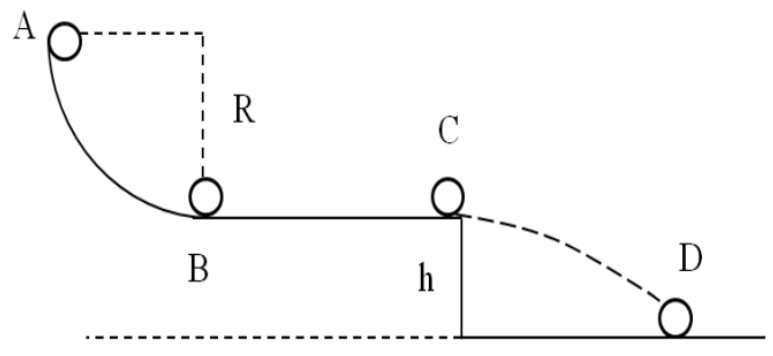
\includegraphics[scale=0.8]{../figs/VN10-2021-PH-TP027-4}
	\end{center}
}
\loigiai{
	
	\begin{enumerate}[label=\alph*)]
		\item Tính vận tốc của vật tại C.
		
		Chọn gốc thế năng tại mặt đất (tại D).
		
		Độ cao điểm A là $z_\text{A} = h + R = \SI{4.4}{m}$.
		
		Độ cao điểm C là $z_\text{C} = h = \SI{2}{m}$.
		
		Áp dụng bảo toàn cơ năng tại A và C:
		$$W_\text{A} = W_\text{C} \Rightarrow 0 + mgz_\text A = \dfrac{1}{2}mv_\text{C}^2 + mgz_\text{C} \Rightarrow v_\text{C} = \xsi{4\sqrt 3}{m/s}.$$
		
		\item Đến C vật rơi ngang và rơi xuống đất. Tính vận tốc của vật khi vật chạm đất.
		
		Áp dụng bảo toàn cơ năng tại C và D, với $z_\text{D} = 0$:
		$$W_\text{C} = W_\text{D} \Rightarrow \dfrac{1}{2}mv_\text{C}^2 + mgz_\text{C} = \dfrac{1}{2} mv_\text{D}^2 + 0 \Rightarrow v_\text{D} = \xsi{2\sqrt{22}}{m/s}.$$
	\end{enumerate}
}
	
\end{enumerate}

\section{Lý thuyết: Biến thiên cơ năng của vật chuyển động trong trọng trường}
\begin{enumerate}[label=\bfseries Câu \arabic*:]
	\item \mkstar{2} [4]
	
	\cauhoi{
		Một vật trượt trên mặt phẳng nghiêng có ma sát, sau khi lên tới điểm cao nhất nó trượt xuống vị trí ban đầu. Trong quá trình chuyển động trên
		\begin{mcq}
			\item công của lực ma sát tác dụng vào vật bằng 0.
			\item tổng công của trọng lực và lực ma sát tác dụng vào vật bằng 0.
			\item công của trọng lực tác dụng vào vật bằng 0.
			\item hiệu giữa công của trọng lực và lực ma sát tác dụng vào vật bằng 0.
		\end{mcq}
	}
	
	\loigiai{
		\textbf{Đáp án: C.}
		
		Một vật trượt trên mặt phẳng nghiêng có ma sát, sau khi lên tới điểm cao nhất nó trượt xuống vị trí ban đầu. Trong quá trình chuyển động trên công của trọng lực tác dụng vào vật bằng 0 vì công của trọng lực khi vật đi lên với khi vật đi xuống trái dấu, cùng độ lớn.
	}

	\item \mkstar{3} [3]

\cauhoi{
	17h30 chiều 28-2, bé N.P.H. ở tầng 12A của tòa nhà 60B Nguyễn Huy Tưởng bò từ trong nhà, trèo ra lan can. Sau đó bé treo mình lơ lửng ở tầng 12A. Lúc này, một số người dân ở tòa bên cạnh phát hiện sự việc đã hô hoán. Một anh thanh niên đứng gần đó phát hiện sự việc nên trèo lên mái che của sảnh và đỡ được bé H. khi bé rơi xuống (\textit{Tuổi Trẻ Online}).
	
	Hành động dũng cảm của anh ấy giúp bảo toàn mạng sống cho cháu bé. Từ hiện tượng trên, học sinh hãy giải quyết bài toán vật lý sau:
	
	Vật $m_1=\SI{20}{kg}$ rơi tự do từ độ cao $h=\SI{40}{m}$ cách mặt đất. Khi đến đất, vật $m_1$ va chạm mềm với $m_2=\SI{60}{kg}$. Hãy tính phần năng lượng bị tiêu hao để làm nóng và làm biến dạng trong va chạm mềm giữa hai vật, biết rằng sau va chạm cả hai vật đều dừng chuyển động. Lấy $g=\SI{10}{m/s^2}$ và bỏ qua sức cản không khí.
}

\loigiai{
	
	Coi như vật $m_2$ nằm sát mặt đất, tổng cơ năng của hệ $m_1$ và $m_2$ lúc chưa xảy ra va chạm là:
	$$W = W_1 + W_2 = m_1gh = \SI{8000}{J}.$$
	
	Tổng cơ năng của hệ sau khi va chạm:
	$$W' = 0.$$
	
	Độ biến thiên cơ năng bằng phần năng lượng bị tiêu hao, do đó:
	$$\Delta W = \SI{8000}{J}.$$
}
	
	\item \mkstar{3} [6]

\cauhoi{
	Một vật khối lượng $\SI{2}{kg}$ được ném thẳng đứng với vận tốc ban đầu $\SI{20}{m/s}$ xuống đất. Lấy $g=\SI{10}{m/s^2}$. Chọn gốc thế năng tại mặt đất. Bỏ qua lực cản của không khí trong quá trình vật chuyển động. Sau khi chạm đất, vật lún sâu $\SI{10}{cm}$ rồi dừng lại. Tính lực cản của đất.
	
}
\loigiai{
	
	Cơ năng của vật tại ví trí ném:
	$$W_1 = W_\text{đ 1} + W_\text{t 1} = \SI{400}{J}.$$
	
	Cơ năng của vật tại vị trí sâu $\SI{10}{cm}$ dưới đất:
	$$W_2 = 0 + mgz_2 = \SI{-2}{J}.$$
	
	Khi vật dừng lại thì toàn bộ cơ năng chuyển thành công của lực cản của đất:
	$$\Delta W = W_2 - W_1 = \SI{-402}{J}= A_\text{cản} = -F_\text{cản} \cdot \SI{0.1}{m} \Rightarrow F_\text{cản} = \SI{4020}{N}.$$
	
}

	\item \mkstar{3} [11]

\cauhoi{
	Ném vật khối lượng $\SI{150}{g}$ thẳng đứng lên cao từ mặt đất với vận tốc $\SI{20}{m/s}$. Bỏ qua sức cản không khí. Cho $g=\SI{10}{m/s^2}$. Chọn gốc thế năng tại mặt đất.
	
	Nếu lực cản của không khí bằng $20\%$ trọng lượng của vật thì độ cao cực đại mà vật đạt được là bao nhiêu?
	
}
\loigiai{
	
	Cơ năng:
	$$W_1 = W_\text{đ 1} + 0 = \SI{30}{J}.$$
	
	Lực cản bằng $20\%$ trọng lượng của vật: $F_\text{cản} = \dfrac{20 mg}{100} = \SI{0.3}{N}$.
	
	Công của lực cản tác dụng lên vật từ khi vật ở mặt đất đến khi vật ở độ cao cực đại $h$:
	$$A_\text{cản} = -F_\text{cản} h.$$
	
	Độ biến thiên cơ năng bằng công của lực cản:
	$$\Delta W = W_2 - W_1 = mgh - W_1 = -F_\text{cản} h \Rightarrow h= \SI{16.67}{m}.$$
}
	
	\item \mkstar{3} [12]

\cauhoi{
	Một viên bi nhỏ khối lượng $\SI{200}{g}$ được ném thẳng đứng xuống dưới từ điểm O có độ cao $\SI{7}{m}$ so với mặt đất với tốc độ ban đầu $\SI{4}{m/s}$. Bỏ qua sức cản của không khí, lấy $g=\SI{10}{m/s^2}$. Giải bài toán bằng phương pháp năng lượng, chọn gốc thế năng tại mặt đất. Đất mềm, viên bi lún thẳng xuống mặt đất thêm một đoạn $\SI{10}{cm}$. Tính lực cản trung bình của đất tác dụng lên viên bi.
	
}
\loigiai{
	
	Cơ năng của vật tại ví trí ném:
	$$W_1 = W_\text{đ 1} + W_\text{t 1} = \SI{15.6}{J}.$$
	
	Cơ năng của vật tại vị trí sâu $\SI{10}{cm}$ dưới đất:
	$$W_2 = 0 + mgz_2 = \SI{-0.2}{J}.$$
	
	Khi vật dừng lại thì toàn bộ cơ năng chuyển thành công của lực cản của đất:
	$$\Delta W = W_2 - W_1 = \SI{-15.8}{J}= A_\text{cản} = -F_\text{c} \cdot \SI{0.1}{m} \Rightarrow F_\text{cản} = \SI{158}{N}.$$
}
	
	\item \mkstar{3} [14]

\cauhoi{
	Một vật có khối lượng $\SI{2}{kg}$ được thả rơi tự do từ độ cao $\SI{2.5}{m}$ so với mặt đất. Lấy $g=\SI{10}{m/s^2}$, bỏ qua mọi lực cản của không khí. Chọn gốc thế năng ở mặt đất.
	
	Khi rơi đến mặt đất, vật va chạm với mặt đất và nảy lên đến độ cao cực đại là $\SI{2}{m}$. Tìm phần cơ năng đã mất đi sau khi vật va chạm với mặt đất.
	
}

\loigiai{
	
	Cơ năng lúc thả vật (cơ năng trước khi vật va chạm với mặt đất):
	$$W_1 = mgz_1 = \SI{50}{J}.$$
	
	Cơ năng lúc vật nảy lên đến độ cao cực đại (cơ năng sau khi vật va chạm với mặt đất):
	$$W_2 = mgz_2 = \SI{40}{J}.$$
	
	Phần cơ năng đã mất đi: $$\Delta W = |W_2 - W_1| = \SI{10}{J}.$$
}

	\item \mkstar{3} [15]

\cauhoi{
	\begin{minipage}[l]{0.7\textwidth}
		Vào tháng 1 năm 2020 tại trường THPT Lương Thế Vinh đã diễn ra cuộc thi đua xe thế năng dành cho học sinh khối 10 và khối 7. Cuộc thi đã diễn ra thành công, các học sinh thì hết sức hào hứng và có những trải nghiệm đáng nhớ.
		\begin{enumerate}[label=\alph*)]
			\item Trong cuộc đua, xe của các đội có thể được đặt thêm những thể tích chất lỏng khác nhau. Việc lựa chọn thể tích chất lỏng đặt vào xe có ảnh hưởng đến quãng đường xe đi được không? Tại sao?
			\item Dốc nghiêng được sử dụng để đua có độ dài $\SI{1.2}{m}$ và cao $\SI{40}{cm}$. Thân xe có khối lượng $\SI{1}{kg}$, lực ma sát xuất hiện trên mặt đất và dốc nghiêng không đổi và có độ lớn bằng $\SI{1.3}{N}$. Lấy $g=\SI{10}{m/s^2}$.
			
			Theo khảo sát, mối liên hệ giữa vận tốc của xe ở chân dốc và độ xa xe chạy được (kể từ chân dốc) được thống kê trong bảng phía dưới.
			\begin{center}
				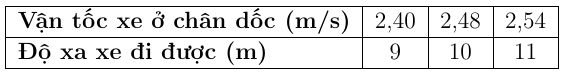
\includegraphics{../figs/VN10-2021-PH-TP027-7}
			\end{center}
			Dùng phương pháp năng lượng để giải quyết vấn đề sau đây: Bạn Thủy mong muốn xe của mình đạt được độ xa $\SI{10}{m}$ thì bạn cần phải đổ vào xe một lượng nước bao nhiêu? Cho rằng 1 lít nước bằng 1 kg.
		\end{enumerate}
	\end{minipage}
	\begin{minipage}[r]{0.3\textwidth}
		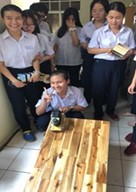
\includegraphics{../figs/VN10-2021-PH-TP027-2}
		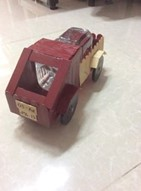
\includegraphics[scale=0.97]{../figs/VN10-2021-PH-TP027-6}
	\end{minipage}
}
\loigiai{
	
	\begin{enumerate}[label=\alph*)]
		\item Việc lựa chọn thể tích chất lỏng đặt vào xe (thay đổi khối lượng xe) không ảnh hưởng đến quãng đường xe đi được. Xét trên quãng đường xe đi được từ vị trí chân dốc đến khi xe dừng lại, theo định lý biến thiên cơ năng, khối lượng của vật ở cả 2 vế của định lý triệt tiêu nhau:
		$$0 - \dfrac{1}{2}mv_1^2 = - \mu mg s$$
		
		\item Để xe đi được độ xa $s=\SI{10}{m}$ thì theo bảng thống kê, vận tốc xe ở chân dốc phải là $v_1 = \SI{2.48}{m/s}$.
		
		Chọn gốc thế năng tại chân dốc. Áp dụng biến thiên cơ năng cho xe lúc ở chân dốc và lúc ở độ xa $\SI{10}{m}$:
		$$\Delta W = W_2 - W_1 = A_\text{ms} \Rightarrow (0+0) - (\dfrac{1}{2}mv_1^2 + 0) = -F_\text{ms} s \Rightarrow m = \SI{4.23}{kg}.$$
		
		Mà thân xe nặng $\SI{1}{kg}$ nên thể tích nước cần đổ vào xe là $\SI{3.23}{kg}$, tương ứng $\SI{3.23}{l}$ nước.
	\end{enumerate}
}

	\item \mkstar{3} [21]

\cauhoi{
	Ném một vật thẳng đứng lên trên với vận tốc $\SI{5}{m/s}$ từ độ cao $\SI{1.5}{m}$ so với mặt đất. Bỏ qua mọi lực cản, cho $g=\SI{10}{m/s^2}$.
	\begin{enumerate}[label=\alph*)]
		\item Tính độ cao cực đại mà vật đạt được và quãng đường mà vật đi được từ khi đạt độ cao cực đại đến khi vật có thế năng bằng 4 lần động năng.
		\item Khi vật đến mặt đất tại điểm D, do đất mềm nên vật lún vào đất $\SI{20}{cm}$. Tính công của lực cản trung bình của đất tác dụng lên vật. Biết khối lượng vật bằng $\SI{400}{g}$.
	\end{enumerate}
}

\loigiai{
	\begin{enumerate}[label=\alph*)]
		\item Tính độ cao cực đại mà vật đạt được và quãng đường mà vật đi được từ khi đạt độ cao cực đại đến khi vật có thế năng bằng 4 lần động năng.
		
		Chọn gốc thế năng tại mặt đất. Áp dụng bảo toàn cơ năng tại vị trí ném và vị trí độ cao cực đại:
		$$W_\text{A} = W_\text{B} \Rightarrow \dfrac{1}{2}mv_\text{A}^2 + mgz_\text{A} = 0 + mgz_\text{B} \Rightarrow z_\text{B} = \SI{2.75}{m}.$$
		
		Khi vật có thế năng bằng 4 lần động năng $W_\text{t C} = 4 W_\text{đ C}$ thì $W_\text{C} = \dfrac{W_\text{t C}}{4} + W_\text{C} = \dfrac{5 W_\text{t C}}{4}$. Áp dụng bảo toàn cơ năng:
		$$W_\text{A} = W_\text{C} \Rightarrow \dfrac{1}{2}mv_\text{A}^2 + mgz_\text{A} = \dfrac{5 mgz_\text{C}}{4}  \Rightarrow z_\text{C} = \SI{2.2}{m}.$$
		
		Vậy quãng đường vật đi được từ khi đạt độ caoc cực đại đến khi vật có thế năng bằng 4 lần động năng là $s=z_\text{B} - z_\text{C} = \SI{0.55}{m}$.
		
		\item Khi vật đến mặt đất tại điểm D, do đất mềm nên vật lún vào đất $\SI{20}{cm}$. Tính công của lực cản trung bình của đất tác dụng lên vật. Biết khối lượng vật bằng $\SI{400}{g}$.
		
		Cơ năng tại điểm D có $z_\text{D} = \SI{-0.2}{m}$: $W_\text{D} = mgz_\text{D} = \SI{-0.8}{J}$
		
		Độ biến thiên cơ năng bằng công của lực cản:
		$$A_\text{cản} = \Delta W = W_\text{D} - W_\text{A} = \SI{-11.8}{J}.$$
	\end{enumerate}
}

	\item \mkstar{3} [22]

\cauhoi{
	Một vật có khối lượng $\SI{3}{kg}$ được thả rơi không vận tốc đầu từ độ cao $\SI{4}{m}$ so với mặt đất. Lấy $g=\SI{9.8}{m/s^2}$. Biết ngay trước khi chạm đất vận tốc của vật là $\SI{6}{m/s}$. Hãy tính lực cản trung bình của không khí tác dụng lên vật.
}

\loigiai{
	Chọn gốc thế năng tại mặt đất. Cơ năng vật lúc mới thả vật:
	$$W_1 = 0 + mgz_1 = \SI{117.6}{J}.$$
	
	Cơ năng vật ngay trước khi vật chạm đất:
	$$W_2 = \dfrac{1}{2}mv_2^2 + 0 = \SI{54}{J}.$$
	
	Độ biến thiên cơ năng bằng công của lực cản (với $s=\SI{4}{m}$):
	$$W_2 - W_1 = -F_\text{cản} s \Rightarrow F_\text{cản} = \SI{15.9}{N}.$$
}

	\item \mkstar{3} [28]

\cauhoi{
	Từ tầng 10 của tòa nhà cao tầng cách mặt đất $\SI{35}{m}$, một vật nặng $\SI{200}{g}$ được ném theo hướng xuống với vận tốc $\SI{20}{m/s}$. Chọn mốc thế năng tại mặt đất, bỏ qua mọi ma sát và lực cản của không khí, lấy $g=\SI{10}{m/s^2}$. Khi rơi xuống đất, do đất mềm và lún thì người ta thấy vật lún sâu vào đất một đoạn. Biết lực cản trung bình của đất là $\SI{440}{N}$. Tìm độ sâu vật lún vào đất.
}

\loigiai{
	Cơ năng lúc ném vật:
	$$W_1 = \dfrac{1}{2}mv_1^2 + mgz_1 = \SI{110}{J}.$$
	
	Cơ năng vật lúc vật ở độ sâu $d$ trong đất:
	$$W_2 = -mgd.$$
	
	Độ biến thiên cơ năng bằng công của lực cản:
	$$W_2 - W_1 = -F_\text{c} d \Rightarrow -mgd - W_1 = -F_\text{c} d \Rightarrow d = \SI{0.25}{m}.$$
	
	Vậy độ sâu vật lún vào đất là $d=\SI{0.25}{m}$.
}

	\item \mkstar{3} [31]

\cauhoi{
	Một vật trượt không vận tốc đầu từ đỉnh mặt phẳng nghiêng cao $\SI{1.25}{m}$. Cho gia tốc rơi tự do $g=\SI{10}{m/s^2}$.
	\begin{enumerate}[label=\alph*)]
		\item Vật trượt không ma sát trên mặt phẳng nghiêng. Hãy tính vận tốc của vật tại chân mặt phẳng nghiêng.
		\item Khi đến chân mặt phẳng nghiêng, vật tiếp tục trượt trên mặt phẳng nằm ngang nối liền với mặt nghiêng. Thời gian chuyển động của vật trên mặt phẳng ngang là $\SI{5}{s}$. Tính hệ số ma sát giữa vật và mặt phẳng nằm ngang.
	\end{enumerate}
	
}
\loigiai{
	
	\begin{enumerate}[label=\alph*)]
		\item Vật trượt không ma sát trên mặt phẳng nghiêng. Hãy tính vận tốc của vật tại chân mặt phẳng nghiêng.
		
		Chọn gốc thế năng tại mặt đất. Bảo toàn cơ năng tại đỉnh dốc và chân dốc:
		$$W_1 = W_2 \Rightarrow 0 + mgz_1 = \dfrac{1}{2}mv_2^2 + 0 \Rightarrow v_2 = \SI{5}{m/s}.$$
		
		\item Khi đến chân mặt phẳng nghiêng, vật tiếp tục trượt trên mặt phẳng nằm ngang nối liền với mặt nghiêng. Thời gian chuyển động của vật trên mặt phẳng ngang là $\SI{5}{s}$. Tính hệ số ma sát giữa vật và mặt phẳng nằm ngang.
		
		Gia tốc của vật trên mặt nghiêng:
		$$v_3 = 0 = at + v_2 \Rightarrow a = \SI{-1}{m/s^2}.$$
		
		Quãng đường vật trượt trên mặt ngang:
		$$s=\dfrac{1}{2}at^2 + v_2 t = \SI{12.5}{m}.$$
		
		Độ biến thiên cơ năng bằng công của lực ma sát:
		$$W_3 - W_2 = -\mu mg s \Rightarrow 0 - \dfrac{1}{2}mv_2^2 = -\mu mg s \Rightarrow \mu = \SI{0.1}{}.$$	
		
	\end{enumerate}
}
	\item \mkstar{4} [2]

\cauhoi{
	\begin{minipage}[l]{0.6\textwidth}
		
		Một vật lăn lên dốc từ A với vận tốc $\SI{10}{m/s}$, vật dừng lại ở B rồi lăn xuống dốc theo đường cũ. Tốc độ vật khi xuống chân dốc ở A là $\SI{6}{m/s}$. Cho $g=\SI{10}{m/s^2}$ và hệ số ma sát $\mu = \SI{0.1}{}$. Tìm AC.
		
	\end{minipage}
	\begin{minipage}[r]{0.4\textwidth}
		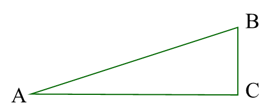
\includegraphics[scale=0.7]{../figs/VN10-2021-PH-TP027-5}
	\end{minipage}
}

\loigiai{
	
	Độ biến thiên cơ năng của vật trong suốt quá trình chuyển động:
	$$\Delta W = \dfrac{1}{2} m (v_2^2 - v_1^2)=-32m.$$
	
	Công của lực ma sát trong quá trình vật chuyển động lên (với $l=\text{AB}$):
	
	$$A_\text{ms 1} = -\mu mg \cos \alpha l.$$
	
	Công của lực ma sát trong quá trình vật chuyển động xuống:
	$$A_\text{ms 2} = -\mu mg \cos \alpha l.$$
	
	Công của lực ma sát trong suốt quá trình:
	$$A_\text{ms} = - 2\mu mg \cos \alpha l.$$
	
	Mà độ biến thiên cơ năng bằng công của lực ma sát, suy ra
	$$\Delta W = -32m = - 2\mu mg \cos \alpha l \Rightarrow 32 =\mu g \cos \alpha l.$$
	
	Lại có $\cos \alpha = \dfrac{\text{AC}}{l}$ nên:
	$$32 =\mu g \dfrac{\text{AC}}{l} l = \mu g \text{AC} \Rightarrow \text{AC} = \SI{32}{m}.$$
}

\end{enumerate}

	\section{Lý thuyết: Bảo toàn cơ năng của vật chuyển động chịu tác dụng của lực đàn hồi}
	\begin{enumerate}[label=\bfseries Câu \arabic*:]
		
				\item \mkstar{3} [1]
		
		\cauhoi{
			Một lò xo nhẹ có độ cứng $k=\SI{50}{N/m}$, một đầu cố định, đầu còn lại gắn vào vật khối lượng $m=\SI{100}{g}$. Vật có thể chuyển động không ma sát trên mặt sàn nằm ngang song song với trục lò xo. Từ vị trí cân bằng người ta kéo vật ra khỏi vị trí cân bằng một đoạn $x_1$ và thả nhẹ cho vật chuyển động. Khi vật đến vị trí cân bằng, vật có tốc độ $\xsi{20\sqrt 5}{cm/s}$. Tìm $x_1$ và độ lớn lực đàn hồi tại vị trí lò xo dãn $x_1$.
		}
		
		\loigiai{
			Cơ năng của hệ tại vị trí thả vật:
			$$W_1 = \dfrac{1}{2}kx_1^2 +0 = \dfrac{1}{2}kx_1^2.$$
			
			Cơ năng của hệ tại vị trí vật trở lại vị trí cân bằng (với $v=\xsi{0.2\sqrt5}{m/s}$):
			$$W_2 = 0 + \dfrac{1}{2}mv^2 = \dfrac{1}{2}mv^2.$$
			
			Bảo toàn cơ năng:
			$$W_1 = W_2 \Rightarrow \dfrac{1}{2}kx_1^2 = \dfrac{1}{2}mv^2 \Rightarrow x_1 = \SI{2}{cm}.$$
			
			Lực đàn hồi tại vị trí lò xo dãn $\SI{0.02}{m}$:
			$$F_\text{đh} = -kx_1 = \SI{-1}{N}.$$
		}
	
		\item \mkstar{3} [14]
	
	\cauhoi{
		Một hệ gồm lò xo có độ cứng $\SI{100}{N/m}$ gắn với vật nhỏ có khối lượng $\SI{500}{g}$. Hệ được đặt trên mặt bàn nằm ngang, đầu còn lại của lò xo được gắn vào điểm cố định, kéo vật để lò xo dãn ra $\SI{4}{cm}$ rồi thả nhẹ không vận tốc đầu. Bỏ qua lực ma sát giữa vật và mặt bàn, chọn gốc thế năng tại vị trí lò xo không biến dạng. Tìm thế năng đàn hồi của lò xo tại vị trí buông vật và tính công của lực đàn hồi đã thực hiện khi vật di chuyển từ vị trí được thả đến vị trí lò xo dãn $\SI{2}{cm}$.
	}
	
	\loigiai{
		
		Thế năng đàn hồi của lò xo tại vị trí buông vật (với $\Delta l_1 = \SI{0.04}{m}$):
		
		$$W_\text{t 1} = \dfrac{1}{2}k(\Delta l_1)^2 = \SI{0.08}{J}.$$
		
		Công của lực đàn hồi bằng độ giảm thế năng (với $\Delta l_2 = \SI{0.02}{m}$):
		
		$$A=W_\text{t 1} - W_\text{t 2} =\dfrac{1}{2}k(\Delta l_1^2 - \Delta l_2^2) =\SI{0.06}{J}.$$
	}

		\item \mkstar{4} [1]
		
		\cauhoi{
		Khối gỗ $M=\SI{4}{kg}$ nằm trên mặt phẳng nằm ngang trơn nhẵn, nối với tường bằng lò xo có độ cứng $k=\SI{100}{N/m}$, trục lò xo song song với mặt phẳng nằm ngang. Viên đạn $m=\SI{10}{g}$ bay theo phương ngang với vận tốc $v_0$ song song với trục của lò xo đến đập vào và dính trong gỗ. Sau va chạm, lò xo bị nén một đoạn tối đa là $\Delta l = \SI{30}{cm}$. Tìm $v_0$.	
		}
		
		\loigiai{
				Áp dụng định luật bảo toàn động lượng trước và sau va chạm cho hệ viên đạn - khối gỗ:
				$$\vec p_1 = \vec p_2 \Rightarrow mv_0 + 0 = (M+m)V \Rightarrow V = \dfrac{v_0}{401}.$$
				
				Cơ năng của hệ ngay sau khi va chạm:
				$$W_1 = W_\text{đ 1} + 0 = \dfrac{1}{2} (M+m)V^2.$$
				
				Cơ năng của hệ khi lò xo bị nén một đoạn $\Delta l = \SI{30}{cm}$:
				$$W_2 = 0 + W_\text{t 2} = \dfrac{1}{2} k (\Delta l)^2.$$
				
				Vì bỏ qua ma sát, áp dụng bảo toàn cơ năng:
				$$W_1 = W_2 \Rightarrow \dfrac{1}{2} (M+m)V^2 = \dfrac{1}{2} k (\Delta l)^2 \Rightarrow \dfrac{1}{2} (M+m) \cdot \left(\dfrac{v_0}{401}\right)^2 =  \dfrac{1}{2} k (\Delta l)^2 \Rightarrow v_0 \approx \SI{600.75}{m/s}.$$
		}
	

	
		\item \mkstar{4} [7]
		
		\cauhoi{
			Một lò xo có chiều dài tự nhiên $l_0=\SI{25}{cm}$ đặt trên mặt phẳng nằm ngang. Một đầu lò xo cố định, đầu kia gắn với vật nhỏ $m_1$. Ban đầu giữ vật $m_1$ tại vị trí mà lò xo bị nén một đoạn $\SI{8}{cm}$, đặt vật nhỏ $m_2$ (với $m_2=3m_1$) trên mặt phẳng nằm ngang sát với vật $m_1$. Buông nhẹ để hai vật bắt đầu chuyển động theo phương của trục lò xo. Bỏ qua mọi ma sát. Tính chiều dài cực đại của lò xo.
		}
		
		\loigiai{
			
			Cơ năng ban đầu của hệ:
			$$W_1 = \dfrac{1}{2}kx^2.$$
			
			Hệ bao gồm vật $m_1$ dính với $m_2$ chuyển động cùng nhau từ lúc buông nhẹ đến khi hệ ở vị trí lò xo không biến dạng. Tại vị trí lò xo không biến dạng thì vật $m_2$ tách khỏi $m_1$, khi đó hệ chỉ còn vật $m_2$ và ta không xét đến vật $m_1$ nữa.
			
			Cơ năng của hệ tại vị trí cân bằng ngay trước khi $m_2$ tách ra:
			$$W_2 = \dfrac{1}{2} (m_1+m_2)v^2 = \dfrac{1}{2} (4m_1) v^2.$$
			
			Cơ năng của hệ tại vị trí cân bằng ngay sau khi $m_2$ tách ra:
			$$W_2' = \dfrac{1}{2}m_1v^2.$$
			
			Vậy $W_2'= \dfrac{W_2}{4} = \dfrac{W_1}{4}$, suy ra:
			$$\dfrac{1}{2}k x'^2 = \dfrac{1}{4} \cdot \dfrac{1}{2}kx^2 \Rightarrow x'^2 = \dfrac{1}{4}x^2 \Rightarrow x'=\SI{4}{cm}.$$
			
			Vậy chiều dài cực đại của lò xo cần tìm là $l_\text{max} = \SI{25}{cm} + \SI{4}{cm} = \SI{29}{cm}$.
		}
	
	\end{enumerate}

\whiteBGstarEnd
	\stopcontents[mychapters]
	
\chapter[\textbf{Ôn tập: Chương IV. Các định luật bảo toàn}]{Ôn tập: Chương IV. Các định luật bảo toàn}
	
	\startcontents[chapters]
	\printcontents[chapters]{}{0}{\setcounter{tocdepth}{1}}
	\whiteBGstarBegin
\setcounter{section}{0}
\section{Động lượng - Định luật bảo toàn động lượng}
\begin{enumerate}[label=\bfseries Câu \arabic*:]
	
	\item \mkstar{1}
	
	\cauhoi{Một vật có khối lượng $m=\SI{1}{\kilogram}$ đang chuyển động với vận tốc $v=\SI{2}{\meter/\second}$. Tính động lượng của vật.
	}
	\loigiai
	{Động lượng của vật: $p=mv=\SI{2}{kg.m/s}$.
	}
	
	\item \mkstar{1}
	
	\cauhoi{Một vật có khối lượng $\SI{2}{\kilogram}$ và có động lượng $\SI{6}{kg.m/s}$. Vật đang chuyển động với vận tốc bao nhiêu?
	}
	\loigiai
	{Vận tốc của vật: $v=\dfrac{p}{m}=\SI{3}{m/s}$.
	}
	\item \mkstar{2}
	
	\cauhoi{Hai vật có khối lượng $m_1=\SI{1}{\kilogram}$, $m_2=\SI{3}{\kilogram}$ chuyển động với các vận tốc $v_1=\SI{3}{\meter/\second}$ và $v_2=\SI{1}{\meter/\second}$. Tìm tổng động lượng (phương, chiều và độ lớn) của hệ trong các trường hợp
		\begin{enumerate}[label=\alph*)]
			\item $\vec{v}_1$ và $\vec{v}_2$ cùng hướng.
			\item $\vec{v}_1$ và $\vec{v}_2$ cùng phương, ngược chiều.
			\item $\vec{v}_1$ và $\vec{v}_2$ vuông góc nhau.
			\item $\vec{v}_1$ và $\vec{v}_2$ hợp nhau một góc $120^\circ$.
		\end{enumerate}
	}
	\loigiai{
		
		\begin{enumerate}[label=\alph*)]
			\item $p=m_1v_1 + m_2v_2 = \SI{6}{kg.m/s}$.
			\item $p=|m_1v_1 - m_2v_2|=0$.
			\item $p=\sqrt{(m_1v_1)^2 + (m_2v_2)^2}=\xsi{3\sqrt2}{kg.m/s}$.
			\item $p=\sqrt{(m_1v_1)^2 + (m_2v_2)^2 + 2(m_1v_1)(m_2v_2)\cos 120^\circ} = \SI{3}{kg.m/s}$.
		\end{enumerate}
	}
\item \mkstar{2}

\cauhoi{Một quả bóng có khối lượng $m=\SI{300}{\gram}$ va chạm vào tường và nảy trở lại với cùng tốc độ. Vận tốc bóng trước va chạm là $\SI{5}{\meter/\second}$. Tìm độ biến thiên động lượng.
	
}
\loigiai{
	
	Độ biến thiên động lượng của quả bóng:
	$\Delta \vec p  = \vec p' - \vec p$.
	
	Vì $\vec p'$ và $\vec p$ cùng phương, ngược chiều nên $\Delta p = -2p = \SI{-3}{kg.m/s}$.
}
\item \mkstar{2}

\cauhoi{Một khẩu súng nằm ngang khối lượng $m_\text{s}=\SI{1000}{\kilogram}$, bắn một viên đạn khối lượng $m_\text{đ}=\SI{10}{\gram}$. Vận tốc viên đạn ra khỏi nòng súng là $\SI{600}{\meter/\second}$. Độ lớn vận tốc của súng sau khi bắn bằng là bao nhiêu?
	
}
\loigiai{
	
	Áp dụng định luật bảo toàn động lượng trước và sau khi bắn:
	$$m_1v_1 + m_2 v_2 = m_1v_1' + m_2 v_2' \Rightarrow 0 + 0 = \SI{1000}{kg} \cdot v_\text s + \SI{0.01}{kg} \cdot \SI{600}{m/s} \Rightarrow v_\text s = \SI{-6e-3}{m/s}$$
	
	Dấu $-$ chứng tỏ súng bị giật lùi.
}

\item \mkstar{2}

\cauhoi{Tên lửa có khối lượng vỏ là 10 tấn chuyển động với vận tốc $\SI{200}{\meter/\second}$ so với Trái Đất, 2 tấn khí phụt ra phía sau có vận tốc $\SI{500}{\meter/\second}$ so với Trái Đất. Xác định vận tốc của tên lửa so với Trái Đất sau khi khí phụt ra.
	
}
\loigiai{
	
	Áp dụng định luật bảo toàn động lượng trước và sau khi khí phụt ra:
	$$(m_1+m_2)v = m_1v_1 + m_2 v_2 \Rightarrow (\SI{10000}{kg} + \SI{2000}{kg}) \cdot \SI{200}{m/s} = \SI{10000}{kg} \cdot v_1 + \SI{2000}{kg} \cdot \SI{-500}{m/s}$$ $$\Rightarrow v_1  =\SI{340}{m/s}$$
}
	\item \mkstar{3}
	
	\cauhoi{Một xe có khối lượng 5 tấn bắt đầu hãm phanh chuyển động thẳng chậm dần đều dừng lại hẳn sau $\SI{20}{\second}$ kể từ lúc bắt đầu hãm phanh, trong thời gian đó xe chạy được $\SI{120}{\meter}$. Tính động lượng của xe lúc bắt đầu hãm phanh.
	}
	\loigiai
	{Vận tốc của xe lúc bắt đầu hãm phanh, giải hệ phương trình:
		
		$$\begin{cases}
			2aS=v^2 - v_0^2 \\
			v=at+v_0
		\end{cases}
		\Rightarrow
		\begin{cases}
			2a\cdot 120 =0 - v_0^2 \\
			0=a\cdot 20 + v_0
		\end{cases}
		\Rightarrow v_0 = \SI{12}{m/s}
		$$
		
		Động lượng của xe lúc bắt đầu hãm phanh: $p=mv_0=\SI{60000}{kg.m/s}$.
	}
	

	

	\item \mkstar{3}
	
	\cauhoi{Một vật có khối lượng $\SI{1}{\kilogram}$ rơi tự do xuống đất trong khoảng thời gian $\SI{0,5}{\second}$. Độ biến thiên động lượng của vật trong khoảng thời gian đó là bao nhiêu? Lấy $g=\SI{10}{\meter/\second^2}$.
		
	}
	\loigiai{
		
		Độ biến thiên vận tốc của vật:
		$\Delta v = gt = \SI{4.9}{m/s}$.
		
		Độ biến thiên động lượng của vật: $\Delta p = m\Delta v = \SI{4.9}{kg.m/s}$.
	}
	
		
	\item \mkstar{3}
	
	\cauhoi{Một quả bóng $\SI{2.5}{\kilogram}$ đập vào tường với vận tốc $\SI{8.5}{\meter/\second}$ và bị bật ngược trở lại với vận tốc $\SI{7.5}{m/s}$. Biết thời gian va chạm là $\SI{0.25}{\second}$. Tìm lực mà tường tác dụng lên quả bóng.
		
	}
	\loigiai{
		
		Độ biến thiên động lượng của quả bóng:
		$\Delta p = \SI{-40}{kg.m/s}$.
		
		Lưc mà tường tác dụng lên quả bóng: $F=\dfrac{\Delta p}{\Delta t} = \SI{-160}{N}$.
	}
	
	\item \mkstar{3}
	
	\cauhoi{Một toa xe khối lượng 10 tấn đang chuyển động trên đường ray nằm ngang với vận tốc không đổi $v=\SI{54}{\kilo\meter/\hour}$, người ta tác dụng lên toa xe một lực hãm theo phương ngang. Tính độ lớn trung bình của lực hãm nếu toa xe dừng lại sau
		\begin{enumerate}[label=\alph*)]
			\item 1 phút 40 giây.
			\item 10 giây.
		\end{enumerate}
		
	}
	\loigiai{
		
		\begin{enumerate}[label=\alph*)]
			\item $F=\dfrac{\Delta p}{\Delta t}=\SI{1500}{\newton}$.
			\item $F=\dfrac{\Delta p}{\Delta t}=\SI{15000}{\newton}$.
		\end{enumerate}
	}
	
	\item \mkstar{3}
	
	\cauhoi{Một viên đạn khối lượng $\SI{10}{\gram}$ đang bay với vận tốc $\SI{600}{\meter/\second}$ thì gặp một bức tường. Đạn xuyên qua tường trong thời gian $\dfrac{1}{100}\,\text{s}$. Sau khi xuyên qua tường, vận tốc của đạn còn $\SI{200}{\meter/\second}$. Tính lực cản của tường tác dụng lên viên đạn.
		
	}
	\loigiai{
		Độ biến thiên động lượng của viên đạn:
		$\Delta p = m\Delta v = \SI{4}{kg.m/s}$.
		
		Lực cản của tường tác dụng lên viên đạn: $F=\dfrac{\Delta p}{\Delta t} = \SI{400}{N}$.
	}
	
	
	
	\item \mkstar{3}
	
	\cauhoi{Vật $m_1$ chuyển động với vận tốc $\SI{6}{\meter/\second}$ đến va chạm với vật $m_2$ chuyển động ngược chiều với vận tốc $\SI{2}{\meter/\second}$. Sau va chạm, hai vật bật ngược trở lại với vận tốc $\SI{4}{\meter/\second}$. Tính khối lượng của hai vật biết $m_1+m_2=\SI{ 1,5}{\kilogram}$.
		
	}
	\loigiai{
		
		Ta có $m_1+m_2=\SI{ 1,5}{\kilogram}$.
		
		Áp dụng định luật bảo toàn động lượng trong va chạm đàn hồi:
		$$m_1v_1 + m_2 v_2 = m_1v_1' + m_2 v_2' \Rightarrow m_1\cdot\SI{6}{m/s} + m_2 \cdot \SI{-2}{m/s} = m_1 \cdot \SI{-4}{m/s} + m_2 \cdot \SI{4}{m/s}.$$
		
		Giải hệ 2 phương trình trên, thu được
		$\begin{cases}
			m_1=\SI{0,5625}{\kilogram}\\
			m_2=\SI{0,9375}{\kilogram}.
		\end{cases}$
	}
	
	\item \mkstar{3}
	
	\cauhoi{Vật $\SI{200}{\gram}$ chuyển động với vận tốc $\SI{6}{\meter/\second}$ đến va chạm với vật $\SI{50}{\gram}$ chuyển động với vận tốc $\SI{4}{\meter/\second}$. Sau va chạm vật $\SI{200}{\gram}$ giữ nguyên hướng và chuyển động với vận tốc bằng nửa vận tốc ban đầu. Tính vận tốc của vật còn lại trong các trường hợp sau:
		\begin{enumerate}[label=\alph*)]
			\item Trước va chạm hai vật chuyển động cùng chiều.
			\item Trước va chạm hai vật chuyển động ngược chiều.
		\end{enumerate}
		
	}
	\loigiai{
		
		\begin{enumerate}[label=\alph*)]
			\item Trước va chạm hai vật chuyển động cùng chiều.
			
			Áp dụng định luật bảo toàn động lượng trong va chạm đàn hồi:
			$$m_1v_1 + m_2 v_2 = m_1v_1' + m_2 v_2' \Rightarrow \SI{0.2}{kg} \cdot \SI{6}{m/s} + \SI{0.05}{kg} \cdot \SI{4}{m/s} = \SI{0.2}{kg} \cdot \SI{3}{m/s} + \SI{0.05}{kg} \cdot v_2'$$ $$\Rightarrow v_2'=\SI{16}{m/s}$$
			
			\item Trước va chạm hai vật chuyển động ngược chiều.
			
			Áp dụng định luật bảo toàn động lượng trong va chạm đàn hồi:
			$$m_1v_1 + m_2 v_2 = m_1v_1' + m_2 v_2' \Rightarrow \SI{0.2}{kg} \cdot \SI{6}{m/s} + \SI{0.05}{kg} \cdot \SI{-4}{m/s} = \SI{0.2}{kg} \cdot \SI{3}{m/s} + \SI{0.05}{kg} \cdot v_2'$$ $$\Rightarrow v_2'=\SI{8}{m/s}$$
		\end{enumerate}
	}
	
	
\item \mkstar{4}

\cauhoi{Từ độ cao $h=\SI{80}{\meter}$, ở thời điểm $t_0=0$ một vật $\SI{200}{\gram}$ được ném ngang với vận tốc ban đầu $v_0=10\sqrt{3}\,\text{m/s}$, gia tốc trọng trường $g=\SI{10}{\meter/\second^2}$. Tìm động lượng của vật ở thời điểm $t=\SI{1}{\second}$.
}
\loigiai
{Tại thời điểm $t=\SI{1}{\second}$, vận tốc theo các phương $x$ và $y$ là
	$$
	\begin{cases}
		v_x=v_0=10\sqrt{3}\,\text{m/s} \\
		v_y=gt=10\,\text{m/s}
	\end{cases}
	$$
	
	Vận tốc của vật tại thời điểm $t=\SI{1}{\second}$: $v=\sqrt{v_x^2 + v_y^2} = \SI{20}{m/s}$.
	
	Động lượng của vật tại thời điểm $t=\SI{1}{\second}$: $p=mv=\SI{4}{kg.m/s}$.
	
}
\item \mkstar{4}

\cauhoi{Xác định độ biến thiên động lượng của một vật có khối lượng $\SI{4}{\kilogram}$ sau khoảng thời gian 6 giây. Biết rằng vật chuyển động trên đường thẳng và có phương trình chuyển động là $x=t^2-6t+3$.
	
}
\loigiai{
	
	Gia tốc của vật: $a=\SI{2}{m/s^2}$.
	
	Vận tốc ban đầu của vật: $v_0 = \SI{-6}{m/s}$.
	
	Độ biến thiên vận tốc của vật:
	$\Delta v = v-v_0 = v_0+at-v_0=at = \SI{12}{m/s}$.
	
	Độ biến thiên động lượng của vật: $\Delta p = m\Delta v = \SI{48}{kg.m/s}$.
}
\end{enumerate}

\section{Công và công suất}
\begin{enumerate}[label=\bfseries Câu \arabic*:]
	
			\item \mkstar{2}
	
	\cauhoi{
		Một vật có khối lượng $m=\SI{500}{\gram}$ trượt từ đỉnh B đến chân C của một mặt phẳng nghiêng có chiều dài $l=\text{BC}=\SI{2}{\meter}$, góc nghiêng $\beta$; $g=\SI{10}{\meter/\second^2}$. Công của trọng lực thực hiện khi vật di chuyển từ B đến C bằng $\SI{4}{\joule}$.
		\begin{center}
			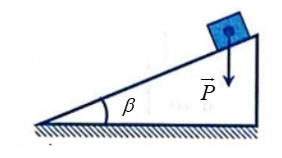
\includegraphics[scale=0.9]{../figs/VN10-PH-30-P-022-1-H1.jpg}
		\end{center}
		Giá trị của $\beta$ xấp xỉ bằng
		\begin{mcq}(4)
			\item $30^\circ$.
			\item $31^\circ$.
			\item $51^\circ$.
			\item $24^\circ$.
		\end{mcq}
		
	}
	
	\loigiai{
		\textbf{Đáp án: D.}
		
		Công của trọng lực:
		$$A=mgh = mg l \sin \beta \Rightarrow \sin \beta = 0,4 \Rightarrow \beta \approx 24^\circ$$
	}
	\item \mkstar{3}
	
	\cauhoi{
		Một vật khối lượng $m=\SI{10}{\kilogram}$ được kéo chuyển động thẳng nhanh dần dều trên sàn nhẵn không ma sát bằng một lực $F=\SI{5}{\newton}$ theo phương ngang từ trạng thái nghỉ. Trong thời gian 4 giây tính từ lúc bắt đầu chuyển động công suất trung bình của lực $F$ bằng
		\begin{mcq}(4)
			\item $\SI{10}{\watt}$.
			\item $\SI{8}{\watt}$.
			\item $\SI{5}{\watt}$.
			\item $\SI{4}{\watt}$.
		\end{mcq}
		
	}
	
	\loigiai{
		\textbf{Đáp án: D.}
		
		Gia tốc vật thu được:
		$$a=\dfrac{F}{m} = \SI{0.5}{m/s^2}$$
		
		Quãng đường vật đi được:
		$$s=\dfrac{1}{2}at^2 = \SI{4}{m}$$
		
		Công của lực $F$:
		$$A=Fs= \SI{20}{J}$$
		
		Công suất trung bình của lực $F$:
		$$\calP = \dfrac{A}{t} = \SI{5}{W}$$
	}
	\item \mkstar{4}
	
	\cauhoi{
		Một người kéo một vật có $m=\SI{8}{\kilogram}$ trượt trên mặt phẳng ngang có hệ số ma sát $\mu=0,2$ bằng một sợi dây có phương hợp một góc $60^\circ$ so với phương nằm ngang. Lực tác dụng lên dây bằng $\vec{F}_\text{k}$, vật trượt không vận tốc đầu với $a=\SI{1}{\meter/\second^2}$. Công của lực kéo trong thời gian 4 giây kể từ khi bắt đầu chuyển động là (lấy $g=\SI{10}{m/s^2}$)
		\begin{mcq}(4)
			\item $\SI{162,5}{\joule}$.
			\item $\SI{140,7}{\joule}$.
			\item $\SI{142,6}{\joule}$.
			\item $\SI{126,7}{\joule}$.
		\end{mcq}
		
	}
	
	\loigiai{
		\textbf{Đáp án: C.}
		
		Quãng đường vật đi được trong 4 giây:
		$$s=\dfrac{1}{2}at^2 = \SI{8}{m}$$
		
		Áp dụng định luật II Newton theo phương thẳng đứng:
		$$F_y + N =P\Rightarrow N = mg -F_y = mg - F \sin \alpha$$
		
		Áp dụng định luật II Newton theo phương ngang:
		$$F_x - F_\text{ms} = ma \Rightarrow F \cos \alpha - F_\text{ms} = ma \Rightarrow F \cos \alpha -  \mu (mg - F \sin \alpha) = ma$$
		
		Tìm được độ lớn lực $F$:
		$$F=\SI{35,65}{N}$$
		
		Công của lực kéo:
		$$A=Fs\cos \alpha  = \SI{142.6}{J}$$
	}
	
	\item \mkstar{4}
	
	\cauhoi{
		Một vật có khối lượng $m=\SI{3}{\kilogram}$ được kéo lên trên mặt phẳng nghiêng một góc $30^\circ$ so với phương ngang bởi một lực không đổi $F=\SI{70}{\newton}$ dọc theo mặt phẳng nghiêng. Biết hệ số ma sát là 0,05, lấy $g=\SI{10}{\meter/\second^2}$. Tổng công của tất cả các lực tác dụng lên vật là $\SI{215}{\joule}$.
		\begin{center}
			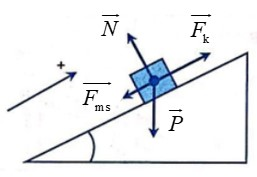
\includegraphics[scale=0.9]{../figs/VN10-PH-30-P-022-1-H2.jpg}
		\end{center}
		Quãng đường tương ứng vật đã di chuyển bằng
		\begin{mcq}(4)
			\item $\SI{1}{\meter}$.
			\item $\SI{2}{\meter}$.
			\item $\SI{4}{\meter}$.
			\item $\SI{6}{\meter}$.
		\end{mcq}
		
	}
	
	\loigiai{
		\textbf{Đáp án: C.}
		
		Phản lực $\vec N$ vuông góc với mặt nghiêng nên công bằng $0$.
		
		Công của trọng lực là công cản: 
		$$A_1=-mgh = -mgs\sin \alpha$$
		
		Công của lực kéo là công phát động:
		$$A_2 = Fs$$
		
		Công của lực ma sát là công cản:
		$$A_3= -\mu N s = -\mu mg \cos \alpha s$$
		
		Tổng công các lực:
		$$A=A_1+A_2+A_3 = \SI{215}{J} \Rightarrow s  =\SI{4}{m}$$
	}

		\item \mkstar{2}
		
		\cauhoi{
			Một ô tô có khối lượng 1,2 tấn chuyển động đều trên mặt đường nằm ngang với vận tốc $v=\SI{36}{\kilo\meter/\hour}$. Hỏi phải thực hiện một công là bao nhiêu để hãm xe dừng lại?
		}
		
		\loigiai{
			Áp dụng công thức:
			$$2as = v^2 - v_0^2 \Rightarrow as=\dfrac{0-10^2}{2}$$
			
			Công của lực thực hiện để xe dừng lại:
			$$A=Fs = mas =\SI{-60000}{J} $$
		}

\item \mkstar{3}

\cauhoi{
	Một xe tải có khối lượng 2,5 tấn bắt đầu chuyển động thẳng nhanh dần đều, sau khi đi được quãng đường $\SI{144}{\meter}$ thì xe đạt vận tốc $\SI{12}{\meter/\second}$. Biết hệ số ma sát giữa xe và mặt đường là $\mu=0,04$. Lấy $g= \SI{10}{\meter/\second^2}$.
	\begin{enumerate}[label=\alph*)]
		\item Tính tổng công của các lực tác dụng lên xe trên quãng đường $\SI{144}{\meter}$ đầu tiên.
		\item Tính công suất của lực do động cơ xe hoạt động ở quãng đường nói trên.
		\item Tính hiệu suất hoạt động của động cơ xe.
	\end{enumerate}
}

\loigiai{		
	\begin{enumerate}[label=\alph*)]
		\item Tính tổng công của các lực tác dụng lên xe trên quãng đường $\SI{144}{\meter}$ đầu tiên.
		
		Gia tốc mà xe thu được:
		$$2as = v^2 - v_0^2 \Rightarrow a = \SI{0.5}{m/s^2}$$
		
		Tổng hợp lực tác dụng lên xe:
		$$\Sigma F = ma = \SI{1250}{N}$$
		
		Tổng công các lực tác dụng lên xe:
		$$A=\Sigma F s = \SI{180000}{J}$$
		\item Tính công suất của lực do động cơ xe hoạt động ở quãng đường nói trên.
		
		Công của lực phát động của động cơ xe:
		$$A_F = A-A_\text{ms} = A- (-\mu mg s) = \SI{324000}{J}$$
		
		Thời gian xe chuyển động:
		$$v=at+v_0 \Rightarrow t = \SI{24}{s}$$
		
		Công suất của động cơ:
		$$\calP = \dfrac{A_F}{t} = \SI{13500}{W}$$
		\item Tính hiệu suất hoạt động của động cơ xe.
		
		$$H=\dfrac{A}{A_F} = \SI{55.56}{\percent}$$
	\end{enumerate}
}
\end{enumerate}

\section{Động năng}
\begin{enumerate}[label=\bfseries Câu \arabic*:]
	
		\item \mkstar{1}
	
	\cauhoi{
		Nhận định nào sau đây về động năng là không đúng?
		\begin{mcq}(1)
			\item Động năng là đại lượng vô hướng và luôn dương.
			\item Động năng có tính tương đối, phụ thuộc hệ quy chiếu.
			\item Động năng tỷ lệ thuận với khối lượng và vận tốc của vật.
			\item Động năng là năng lượng của vật đang chuyển động.
		\end{mcq}
	}
	
	\loigiai{
		\textbf{Đáp án: C.}
		
		Động năng tỷ lệ thuận với khối lượng và bình phương vận tốc của vật.
	}
	
	\item \mkstar{2}
	
	\cauhoi{
		Một ô tô có khối lượng 1,5 tấn đang chuyển động thẳng đều trong 2 giờ xe đi được quãng đường $\SI{72}{\kilo\meter}$. Động năng của ô tô này bằng
		\begin{mcq}(4)
			\item $\SI{972}{\joule}$.
			\item $\SI{150}{\kilo\joule}$.
			\item $\SI{75}{\kilo\joule}$.
			\item $\SI{972}{\kilo\joule}$.
		\end{mcq}
	}
	
	\loigiai{
		\textbf{Đáp án: C.}
		
		Vận tốc của ô tô:
		$$v=\dfrac{s}{t} = \SI{10}{m/s}$$
		
		Động năng của ô tô:
		$$W_\text{đ} = \dfrac{1}{2} mv^2 = \SI{75}{kJ}$$
	}
	\item \mkstar{2}
	
	\cauhoi{
		Một ô tô có khối lượng 4 tấn đang chuyển động với vận tốc $\SI{36}{\kilo\meter/\hour}$ thì hãm phanh, sau một thời gian vận tốc giảm còn $\SI{18}{\kilo\meter/\hour}$. Độ biến thiên của động năng của ô tô là
		\begin{mcq}(4)
			\item $\SI{150}{\kilo\joule}$.
			\item $\SI{-150}{\kilo\joule}$.
			\item $\SI{-75}{\kilo\joule}$.
			\item $\SI{75}{\kilo\joule}$.
		\end{mcq}
	}
	
	\loigiai{
		\textbf{Đáp án: B.}
		
		Độ biến thiên động năng:
		$$\Delta W_\text{đ} = \dfrac{1}{2} m (v^2 - v_0^2) = \SI{-150}{kJ}$$
	}
	\item \mkstar{3}
	
	\cauhoi{
		Một hòn đá có khối lượng $m=\SI{200}{\gram}$ rơi tự do không vận tốc đầu từ một điểm cách mặt đất $\SI{45}{\meter}$, tại nơi có gia tốc trọng trường $g= \SI{10}{\meter/\second^2}$. Động năng của hòn đá ngay trước khi chạm đất là
		\begin{mcq}(4)
			\item $\SI{45}{\joule}$.
			\item $\SI{90}{\joule}$.
			\item $\SI{180}{\joule}$.
			\item $\SI{900}{\joule}$.
		\end{mcq}
	}
	
	\loigiai{
		\textbf{Đáp án: B.}
		
		Thời gian rơi:
		$$h=\dfrac{1}{2}gt^2 \Rightarrow t = \SI{3}{s}$$
		
		Vận tốc của hòn đá ngay trước khi chạm đất:
		$$v=gt= \SI{30}{m/s}$$
		
		Động năng hòn đá ngay trước khi chạm đất:
		$$W_\text{đ} = \dfrac{1}{2} mv^2 = \SI{90}{J}$$
	}
\item \mkstar{3}

\cauhoi{
	Một ô tô có khối lượng $\SI{1600}{\kilogram}$ đang chạy với tốc độ $\SI{54}{\kilo\meter/\hour}$ thì người lái xe nhìn thấy một vật cản trước mặt cách khoảng $\SI{10}{\meter}$. Người đó tắt máy và hãm phanh khẩn cấp với lực hãm không đổi là $\SI{2e4}{\newton}$. Xe dừng lại cách vật cản một khoảng bằng
	\begin{mcq}(4)
		\item $\SI{1,2}{\meter}$.
		\item $\SI{1,0}{\meter}$.
		\item $\SI{1,4}{\meter}$.
		\item $\SI{1,5}{\meter}$.
	\end{mcq}
}

\loigiai{
	\textbf{Đáp án: B.}
	
	Quãng đường xe chạy được cho đến khi dừng hẳn theo lý thuyết định lý động năng là
	$$-F_\text{h}s = 0 - \dfrac{1}{2}mv^2 \Rightarrow s = \SI{9}{m}$$
	
	Vậy xe dừng lại cách vật cản một khoảng bằng $\SI{10}{m}-\SI{9}{m}=\SI{1}{m}$.
}
\item \mkstar{3}

\cauhoi{
	Trung tâm bồi dưỡng kiến thức Hà Nội tổ chức một cuộc thi cho các học viên chạy. Có một học viên có trọng lượng $\SI{700}{\newton}$ chạy đều hết quãng đường $\SI{600}{\meter}$ trong $\SI{50}{\second}$. Tìm động năng của học viên đó. Lấy $g= \SI{10}{\meter/\second^2}$.
}

\loigiai{
	Khối lượng của học viên:
	$$m=\dfrac{P}{g} = \SI{70}{kg}$$
	
	Vận tốc chạy của học viên:
	$$v=\dfrac{s}{t} = \SI{12}{m/s}$$
	
	Động năng của học viên:
	$$W_\text{đ} = \dfrac{1}{2}mv^2 = \SI{5040}{J}$$
}

\item \mkstar{2}

\cauhoi{
	Vận động viên Hoàng Xuân Vinh bắn một viên đạn có khối lượng $\SI{100}{\gram}$ bay ngang với vận tốc $\SI{300}{\meter/\second}$ xuyên qua tấm bia bằng gỗ dày $\SI{5}{\centi\meter}$. Sau khi xuyên qua bia gỗ thì đạn có vận tốc $\SI{100}{\meter/\second}$. Tính lực cản của tấm bia gỗ tác dụng lên viên đạn.
}
\loigiai{
	
	Áp dụng định lý động năng:
	$$-F_\text{cản}s = \dfrac{1}{2}m(v^2-v_0^2) \Rightarrow F_\text{cản} = \SI{80000}{N}$$
}

\item \mkstar{3}

\cauhoi{
	Một vật có khối lượng $\SI{2}{\kilogram}$ trượt qua A với vận tốc $\SI{2}{\meter/\second}$ xuống dốc nghiêng AB dài $\SI{2}{\meter}$, cao $\SI{1}{\meter}$. Biết hệ số ma sát giữa vật và mặt phẳng nghiêng là $\mu=\dfrac{1}{\sqrt{3}}$. Lấy $g= \SI{10}{\meter/\second^2}$.
	\begin{enumerate}[label=\alph*)]
		\item Xác định công của trọng lực, công của lực ma sát thực hiện khi vật chuyển dời từ dinh dốc đến chân dốc.
		\item Xác định vận tốc của vật tại chân dốc B.
		\item Tại chân dốc B vật tiếp tục chuyển dộng trên mặt phẳng nằm ngang BC dài $\SI{2}{\meter}$ thì dừng lại. Xác định hệ số ma sát trên đoạn dường BC này.
	\end{enumerate}
}
\loigiai{
	
	\begin{enumerate}[label=\alph*)]
		\item Xác định công của trọng lực, công của lực ma sát thực hiện khi vật chuyển dời từ dinh dốc đến chân dốc.
		
		Góc nghiêng của mặt phẳng nghiêng:
		$$\sin \alpha = \dfrac{h}{l} = \dfrac{1}{2} \Rightarrow \alpha = 30^\circ $$
		
		Công của trọng lực:
		$$A_1 = mgh  = \SI{20}{J}$$
		
		Độ lớn lực ma sát:
		$$F_\text{ms} = \mu N = \mu mg\cos \alpha = \SI{10}{N}$$
		
		Công của lực ma sát:
		$$A_2=-F_\text{ms} l = \SI{-20}{J}$$
		\item Xác định vận tốc của vật tại chân dốc B.
		
		Áp dụng định lý động năng:
		$$A_1+A_2 = \dfrac{1}{2}mv_\text{B}^2 -\dfrac{1}{2}mv_\text{A}^2 =0\Rightarrow v_\text{B} =v_\text A =  \SI{2}{m/s}$$
		\item Tại chân dốc B vật tiếp tục chuyển dộng trên mặt phẳng nằm ngang BC dài $\SI{2}{\meter}$ thì dừng lại. Xác định hệ số ma sát trên đoạn dường BC này.
		
		Áp dụng định lý động năng:
		$$ -\mu_2 mg s_2 = 0-\dfrac{1}{2}mv_\text B^2 \Rightarrow \mu_2 = \SI{0.1}{}$$
	\end{enumerate}
}

\item \mkstar{3}

\cauhoi{
	Một xe có khối lượng 2 tấn chuyên động trên đoạn AB nằm ngang với vận tốc không đổi $\SI{7,2}{\kilo\meter/\hour}$, lấy $g= \SI{10}{\meter/\second^2}$.
	\begin{enumerate}[label=\alph*)]
		\item Đến điểm B thì xe tắt máy và xuống dốc BC nghiêng góc $30^\circ$ so với phương ngang, bỏ qua ma sát. Biết vận tốc tại chân C là $\SI{72}{\kilo\meter/\hour}$. Tìm chiều dài dốc BC.
		\item Tại C xe tiếp tục chuyển động trên đoạn đường nằm ngang CD và đi thêm được $\SI{200}{\meter}$ thì dừng lại. Tìm hệ số ma sát trên đoạn CD.
	\end{enumerate}
}
\loigiai{
	
	\begin{enumerate}[label=\alph*)]
		\item Đến điểm B thì xe tắt máy và xuống dốc BC nghiêng góc $30^\circ$ so với phương ngang, bỏ qua ma sát. Biết vận tốc tại chân C là $\SI{72}{\kilo\meter/\hour}$. Tìm chiều dài dốc BC.
		
		Bỏ qua ma sát, áp dụng định lý động năng:
		$$A_P=\dfrac{1}{2}mv_\text{C}^2 - \dfrac{1}{2}mv_\text{B}^2 \Rightarrow mgl \sin \alpha = \dfrac{1}{2} mv_\text{C}^2 - \dfrac{1}{2}mv_\text{B}^2 \Rightarrow l = \SI{39.6}{m}$$
		\item Tại C xe tiếp tục chuyên động trên đoạn đường nằm ngang CD và đi thêm được $\SI{200}{\meter}$ thì dừng lại. Tìm hệ số ma sát trên đoạn CD.
		
		Áp dụng định lý động năng:
		$$A_\text{ms} = 0- \dfrac{1}{2}mv_\text{C}^2 \Rightarrow -\mu mgs = - \dfrac{1}{2}mv_\text{C}^2 \Rightarrow \mu = \SI{0.1}{}$$
	\end{enumerate}
}

\item \mkstar{4}

\cauhoi{
	Một ô tô có khối lượng 2 tấn đang chuyển dộng trên đường thẳng nằm ngang AB dài $\SI{100}{\meter}$, khi qua A vận tốc ô tô là $\SI{10}{\meter/\second}$ và đến B vận tốc của ô tô là $\SI{20}{\meter/\second}$. Biết độ lớn của lực kéo là $\SI{4000}{\newton}$.
	\begin{enumerate}[label=\alph*)]
		\item Tìm hệ số ma sát $\mu_1$ trên đoạn đường AB.
		\item Đến B thì động cơ tắt máy và lên dốc BC dài $\SI{40}{\meter}$ nghiêng $30^\circ$ so với mặt phẳng ngang. Hệ số ma sát trên mặt dốc là $\mu_2=\dfrac{1}{5\sqrt{3}}$. Hỏi xe có lên đến đỉnh dốc C không?
		\item Nếu đến B với vận tốc trên, muốn xe lên dốc và dừng lại tại C thì phải tác dụng liên tục lên xe một lực có độ lớn bao nhiêu?
	\end{enumerate}
}
\loigiai{
	
	\begin{enumerate}[label=\alph*)]
		\item Tìm hệ số ma sát $\mu_1$ trên đoạn đường AB.
		
		Áp dụng định lý động năng:
		$$-\mu_1 mg s_1 + Fs_1 = \dfrac{1}{2}mv_\text{B}^2 - \dfrac{1}{2}mv_\text{A}^2 \Rightarrow \mu_1 = \SI{0.05}{}$$
		\item Đến B thì động cơ tắt máy và lên dốc BC dài $\SI{40}{\meter}$ nghiêng $30^\circ$ so với mặt phẳng ngang. Hệ số ma sát trên mặt dốc là $\mu_2=\dfrac{1}{5\sqrt{3}}$. Hỏi xe có lên đến đỉnh dốc C không?
		
		Áp dụng định lý động năng từ B đến khi xe dừng lại:
		$$A_\text{ms2}+A_{P2} = 0 - \dfrac{1}{2}mv_\text{B}^2 \Rightarrow -\mu_2 mg \cos \alpha s_2 - mgs_2 \sin \alpha = 0 - \dfrac{1}{2}mv_\text{B}^2 \Rightarrow s_2 = \SI{33.33}{m}$$
		
		Vậy quãng đường tối đa xe lên được là $\SI{33.33}{m}$, mà dốc dài $\SI{40}{m}$ nên xe không lên được đến đỉnh dốc.
		\item Nếu đến B với vận tốc trên, muốn xe lên dốc và dừng lại tại C thì phải tác dụng liên tục lên xe một lực có độ lớn bao nhiêu?
		
		Để xe lên được đến C thì $s_3=\SI{40}{m}$, khi đó:
		$$A_\text{ms3}+A_{P3}+A_F = 0 - \dfrac{1}{2}mv_\text{B}^2 \Rightarrow -\mu_2 mg \cos \alpha s_3 - mgs_3 \sin \alpha +Fs_3= 0 - \dfrac{1}{2}mv_\text{B}^2 \Rightarrow F = \SI{1}{N}$$
	\end{enumerate}
}
\end{enumerate}

\section{Thế năng}
\begin{enumerate}[label=\bfseries Câu \arabic*:]
	
\item \mkstar{1}

\cauhoi{
	Biểu thức nào sau đây không phải biểu thức của thế năng?
	\begin{mcq}(2)
		\item $W_\text{t}=mgh$.
		\item $W_\text t=mg(z_2-z_1)$.
		\item $W_\text t=Ph$.
		\item $W_\text t=\dfrac{1}{2}mgh$.
	\end{mcq}
	
}

\loigiai{
	\textbf{Đáp án: D.}
	
	$\dfrac{1}{2}mgh$ không phải là biểu thức của thế năng.
}
\item \mkstar{1}

\cauhoi{
	Một vật nằm yên (trong hệ quy chiếu đứng yên) có thể có
	\begin{mcq}(4)
		\item thế năng.
		\item vận tốc.
		\item động năng.
		\item động lượng.
	\end{mcq}
	
}

\loigiai{
	\textbf{Đáp án: A.}
	
	Một vật nằm yên không thể có động lượng, động năng, vận tốc, nhưng có thể có thế năng.
}
\item \mkstar{1}

\cauhoi{
	Thế năng của vật nặng $\SI{2}{\kilogram}$ ở đáy một giếng sâu $\SI{10}{\meter}$ so với mặt đất tại nơi có gia tốc $g= \SI{10}{\meter/\second^2}$ là bao nhiêu?
	\begin{mcq}(4)
		\item $\SI{-100}{\joule}$.
		\item $\SI{100}{\joule}$.
		\item $\SI{200}{\joule}$.
		\item $\SI{-200}{\joule}$. 
	\end{mcq}
}

\loigiai{\textbf{Đáp án: D.}
	
	Thế năng trọng trường:
	$$W_\text t= mgz = \SI{-200}{J}$$
	
}
\item \mkstar{1}

\cauhoi{
	Một lò xo bị nén $\SI{5}{\centi\meter}$. Biết độ cứng lò xo $k=\SI{100}{\newton/\meter}$, thế năng của lò xo là
	\begin{mcq}(4)
		\item $\SI{0,125}{\joule}$.
		\item $\SI{0,25}{\joule}$.
		\item $\SI{125}{\joule}$.
		\item $\SI{250}{\joule}$.
	\end{mcq}
	
}

\loigiai{
	\textbf{Đáp án: A.}
	
	Thế năng đàn hồi của lò xo:
	$$W_\text t= \dfrac{1}{2} k (\Delta l)^2 = \SI{0,125}{\joule}$$
}
\item \mkstar{1}

\cauhoi{
	Một lò xo có độ cứng $\SI{100}{\newton/\meter}$, một đầu cố định, đầu kia gắn với vật nhỏ. Khi lò xo bị nén $\SI{4}{\centi\meter}$ thì thế năng đàn hồi của hệ là
	\begin{mcq}(4)
		\item $\SI{800}{\joule}$.
		\item $\SI{0,08}{\joule}$.
		\item $\SI{8}{\joule}$.
		\item $\SI{80}{\joule}$. 
	\end{mcq}
	
}

\loigiai{
	\textbf{Đáp án: A.}
	
	Thế năng đàn hồi của lò xo:
	$$W_\text t= \dfrac{1}{2} k (\Delta l)^2 = \SI{0.08}{\joule}$$
}

\item \mkstar{2}

\cauhoi{
	Một người có khối lượng $\SI{60}{\kilogram}$ đứng trên mặt đất và cạnh một cái giếng nước, lấy $g=$$\SI{10}{\meter/\second^2}$.
	\begin{enumerate}[label=\alph*)]
		\item Tính thế năng của người tại A cách mặt đất $\SI{3}{\meter}$ về phía trên và tại đáy giếng cách mặt đất $\SI{5}{\meter}$ với gốc thế năng tại mặt đất.
		\item Nếu lấy mốc thế năng tại đáy giếng, hãy tính lại kết quả câu trên.
	\end{enumerate}
}

\loigiai{
	
	\begin{enumerate}[label=\alph*)]
		
		\item Tính thế năng của người tại A cách mặt đất $\SI{3}{\meter}$ về phía trên và tại đáy giếng cách mặt đất $\SI{5}{\meter}$ với gốc thế năng tại mặt đất.
		
		Thế năng của người tại A cách mặt đất $\SI{3}{\meter}$ về phía trên (với $h_1=\SI{3}{m})$:
		
		$$W_\text t = mgh_1 = \SI{1800}{J}$$
		
		Thế năng của người tại đáy giếng cách mặt đất $\SI{5}{\meter}$ (với $h_2=\SI{-5}{m}$):
		$$W_\text t = mgh_2 = \SI{-3000}{J}$$
		
		\item Nếu lấy mốc thể năng tại đáy giếng, hãy tính lại kết quả câu trên.
		
		Thế năng của người tại A cách mặt đất $\SI{3}{\meter}$ về phía trên (với $h_3=\SI{8}{m}$):
		$$W_\text t = mgh_3 = \SI{4800}{J}$$
		
		Thế năng của người tại đáy giếng cách mặt đất $\SI{5}{\meter}$ (với $h_4=0$):
		$$W_\text t = mgh_4 = \SI{0}{J}$$
	\end{enumerate}
}



\item \mkstar{2}

\cauhoi{
	Cho một lò xo nằm ngang có độ cứng $k=\SI{100}{\newton/\meter}$. Công của lực đàn hồi thực hiện khi lò xo bị kéo dãn từ $\SI{2}{\centi\meter}$ đến $\SI{4}{\centi\meter}$ là bao nhiêu?	
	
}
\loigiai{
	
	Độ giảm thế năng bằng công của lực thế:
	$$A = W_\text{t 1} - W_\text{t 2} = \dfrac{1}{2} k (\Delta l_1 ^2 - \Delta l_2^2) = \SI{-0.06}{J}$$
}
\item \mkstar{3}

\cauhoi{
	Một học sinh của trung tâm bồi dưỡng kiến thức Hà Nội thả một vật rơi tự do có khối lượng $\SI{500}{\gram}$ từ độ cao $\SI{45}{\meter}$ so với mặt đất, bỏ qua ma sát với không khí, Tính thế năng của vật tại giây thứ hai so với mặt đất. Cho $g= \SI{10}{\meter/\second^2}$.
}

\loigiai{
	Độ cao của vật tại giây thứ hai so với mặt đất:
	$$h_2 = h - \dfrac{1}{2}gt^2 = \SI{25}{m}$$
	
	Thế năng của vật tại giây thứ hai so với mặt đất (gốc thế năng tại mặt đất):
	$$W_\text t = mgh_2 = \SI{125}{J}$$
}

\end{enumerate}

\section{Cơ năng}
\begin{enumerate}[label=\bfseries Câu \arabic*:]
	
	\item \mkstar{2}
	
	\cauhoi{
		Một học sinh ném một vật có khối lượng $\SI{200}{\gram}$ thẳng đứng lên cao với vận tốc ban đầu $\SI{8}{\meter/\second}$ từ độ cao $\SI{8}{\meter}$ so với mặt đất. Lấy $g= \SI{10}{\meter/\second^2}$. Xác định vận tốc của vật khi $W_\text{đ}=2W_\text{t}$.
	}
	
	\loigiai{
		Chọn gốc thế năng tại mặt đất.
		
		Cơ năng ban đầu:
		$$W_1 = W_\text{đ 1} + W_\text{t 1}  = \SI{22.4}{J}$$
		
		Khi $W_\text{đ 2} = 2 W_\text{t 2}$ thì $W_2 = \dfrac{3}{2} W_\text{đ 2}$. Áp dụng bảo toàn cơ năng:
		$$W_1 = W_2 \Rightarrow W_1 = \dfrac{3}{2}\cdot \dfrac{1}{2}mv_2^2 \Rightarrow v_2 = \SI{12.22}{m/s} $$
		
	}
	
	\item \mkstar{2}
	
	\cauhoi{
		Cho một vật có khối lượng $m$. Truyền cho vật một cơ năng là $\SI{37,5}{\joule}$. Khi vật chuyển động ở độ cao $\SI{3}{\meter}$ vật có $W_\text{đ}=\dfrac{3}{2}W_\text{t}$. Xác định khối lượng của vật và vận tốc của vật ở độ cao đó. Lấy $g= \SI{10}{\meter/\second^2}$.
		
	}
	
	\loigiai{
		
		Khi vật có $W_\text{đ 2} = \dfrac{3}{2} W_\text{t 2}$ thì $W_2 = \dfrac{5}{2} W_\text{t 2}$. Áp dụng bảo toàn cơ năng (với $z_2=\SI{3}{m}$):
		$$W_1 = W_2 \Rightarrow \SI{37.5}{J} = \dfrac{5}{2} mgz_2 \Rightarrow m =\SI{0.5}{kg}$$
		
		Mà $W_\text{đ 2} = \dfrac{3}{2} W_\text{t 2}$ nên
		$$\dfrac{1}{2} mv_2^2 = \dfrac{3}{2} \cdot mgz_2 \Rightarrow v_2 = \xsi{3\sqrt{10}}{m/s}$$
	}
	
	\item \mkstar{3}
	
	\cauhoi{
		Một học sinh chơi đùa ở sân thượng có độ cao $\SI{45}{\meter}$, liền cầm một vật có khối lượng $\SI{100}{\gram}$ thả vật rơi tự do xuống mặt đất. Lấy $g= \SI{10}{\meter/\second^2}$.
		\begin{enumerate}[label=\alph*)]
			\item Tính vận tốc của vật khi vật chạm đất.
			\item Tính độ cao của vật khi $W_\text{đ}=2W_\text{t}$.
			\item Tính vận tốc của vật khi $2W_\text{đ}=5W_\text{t}$.
			\item Xác định vị trí để vận có vận tốc $\SI{20}{\meter/\second}$.
			\item Tại vị trí có độ cao $\SI{20}{\meter}$ vật có vận tốc bao nhiêu?
			\item Khi chạm đất, do đất mềm nên vật bị lún sâu $\SI{10}{\centi\meter}$. Tính lực cản trung bình tác dụng lên vật.
		\end{enumerate}
	}
	
	\loigiai{		
		Chọn gốc thế năng tại mặt đất.
		\begin{enumerate}[label=\alph*)]
			\item Tính vận tốc của vật khi vật chạm đất.
			
			Cơ năng vật lúc thả vật:
			$$W_1 = mgz_1 = \SI{45}{J}$$
			
			Cơ năng vật lúc vật chạm đất:
			$$W_2 = \dfrac{1}{2}mv_2^2$$
			
			Bảo toàn cơ năng:
			$$W_1 = W_2 \Rightarrow v_2 = \SI{30}{m/s}$$
			
			\item Tính độ cao của vật khi $W_\text{đ}=2W_\text{t}$.
			
			Khi $W_\text{đ 3} = 2W_\text{t 2}$ thì $W_3 = 3_\text{t 3}$. Áp dụng bảo toàn cơ năng:
			$$W_1=W_3 = 3mgz_3 \Rightarrow z_3 = \SI{15}{m}$$
			
			\item Tính vận tốc của vật khi $2W_\text{đ}=5W_\text{t}$.
			
			Khi $2W_\text{đ 4} = 5W_\text{t 4}$ thì $W_\text{t 4} = \dfrac{2}{5} W_\text{đ 4}$. Khi đó $W_4 = \dfrac{7}{5} W_\text{đ 4}$. Áp dụng bảo toàn cơ năng:
			$$W_1 = W_4 \Rightarrow W_1 = \dfrac{7}{5} \cdot \dfrac{1}{2}mv_4^2 \Rightarrow v_4 \approx \SI{25.35}{m/s}$$
			\item Xác định vị trí để vận có vận tốc $\SI{20}{\meter/\second}$.
			
			Vị trí này vật có động năng $W_\text{đ 5} = \dfrac{1}{2} mv_5^2 = \SI{20}{J}$, do đó vật có thế năng $W_\text{t 5} = W_5 - W_\text{đ 5} = W_1 - W_\text{đ 5} = \SI{25}{J}$. Vậy vật ở vị trí:
			$$\SI{25}{J} = mgz_5 \Rightarrow z_5 = \SI{25}{m}$$
			
			\item Tại vị trí có độ cao $\SI{20}{\meter}$ vật có vận tốc bao nhiêu?
			
			Tại vị trí này vật có thế năng $W_\text{t 6} = mgz_6 = \SI{20}{J}$, vật có động năng $W_\text{đ 6} = W_6 - W_\text{t 6} = \SI{25}{J}$. Vậy vật có tốc độ:
			$$\SI{25}{J} = \dfrac{1}{2} mv_6^2 \Rightarrow v_6 = \xsi{10\sqrt 5}{m/s}$$
			
			\item Khi chạm đất, do đất mềm nên vật bị lún sâu $\SI{10}{\centi\meter}$. Tính lực cản trung bình tác dụng lên vật.
			
			Cơ năng của vật ở vị trí này (với $z_7 = \SI{-0.1}{m}$):
			$$W_7 = mgz_7 = \SI{-0.1}{J}$$
			
			Độ biến thiên cơ năng bằng công của lực cản:
			$$W_7 - W_1 = -F_\text{c} s \Rightarrow F_\text{c} = \SI{451}{N}$$
		\end{enumerate}
	}
	
	
	\item \mkstar{3}
	
	\cauhoi{
		Một viên bi khối lượng $m$ chuyến động ngang không ma sát với vận tốc $\SI{2}{\meter/\second}$ rồi đi lên mặt phẳng nghiêng góc nghiêng $30^\circ$.
		\begin{enumerate}[label=\alph*)]
			\item Tính quãng đường $s$ mà viên bi đi được trên mặt phẳng nghiêng.
			\item Ở độ cao nào thì vận tốc của viên bi giảm còn một nửa?
			\item Khi vật chuyển động được quãng đường là $\SI{0,2}{\meter}$ lên mặt phẳng nghiêng thì vật có vận tốc bao nhiêu?
		\end{enumerate}
	}
	
	\loigiai{
		Chọn gốc thế năng tại chân mặt phẳng nghiêng.
		
	\begin{enumerate}[label=\alph*)]
	\item Tính quãng đường $s$ mà viên bi đi được trên mặt phẳng nghiêng.
	
	Áp dụng bảo toàn cơ năng:
	$$W_1 = W_2 \Rightarrow \dfrac{1}{2}mv_1^2 = mgz_2 \Rightarrow z_2 = \SI{0.2}{m}$$
	
	Quãng đường mà viên bi đi trên mặt phẳng nghiêng:
	$$s=\dfrac{z_2}{\sin \alpha} = \SI{0.4}{m}$$
	
	\item Ở độ cao nào thì vận tốc của viên bi giảm còn một nửa?
	
	Khi $v_3 = \dfrac{1}{2} v_1$ thì $v_3 = \SI{1}{m/s}$. Áp dụng bảo toàn cơ năng:
	$$W_1 = W_3 \Rightarrow \dfrac{1}{2}mv_1^2 = \dfrac{1}{2}mv_3^2 + mgz_3 \Rightarrow z_3 = \SI{0.15}{m}$$
	
	\item Khi vật chuyển động được quãng đường là $\SI{0,2}{\meter}$ lên mặt phẳng nghiêng thì vật có vận tốc bao nhiêu?
	
	Khi đó vật ở độ cao $z_4 = l \sin \alpha = \SI{0.1}{m}$
	
	Áp dụng bảo toàn cơ năng:
	$$W_1 = W_4 \Rightarrow \dfrac{1}{2}mv_1^2 = \dfrac{1}{2}mv_4^2 + mgz_4 \Rightarrow v_4 = \xsi{\sqrt 2}{m/s}$$
\end{enumerate}
	}
	\item \mkstar{3}
	
	\cauhoi{
		Dây treo vật nặng được kéo nghiêng góc bao nhiêu để khi qua vị trí cân bằng lực căng của dây lớn gấp đôi trọng lượng của vật nặng?
	}
	
	\loigiai{
		Lực căng dây tại vị trí cân bằng:
		$$T=mg(3-2\cos(\alpha_0))$$
		
		Vì $T=2P = 2mg$ nên $3-2\cos(\alpha_0) = 2 \Rightarrow \cos \alpha_0 = 0,5 \Rightarrow \alpha_0 = 60^\circ$.
	}
\item \mkstar{3}

\cauhoi{
	Treo vật $m=\SI{1}{\kilogram}$ vào đầu một sợi dây rồi kéo vật khỏi vị trí cân bằng để dây treo hợp với phương thẳng đứng góc $\alpha_0$. Xác định $\alpha_0$, biết trong quá trình này, dây chịu lực căng tối đa $\SI{16}{\newton}$ và $\alpha_0 < 90^\circ$.
}

\loigiai{
	Lực căng dây tối đa khi vật ở vị trí cân bằng, khi đó:
	$$T=mg(3-2\cos(\alpha_0)) = \SI{16}{N} \Rightarrow \cos \alpha_0 =0,7 \Rightarrow \alpha_0=45,57^\circ$$
}
\item \mkstar{3}

\cauhoi{
	Cho một con lắc đơn gồm một sợi dây dài $\SI{320}{\centi\meter}$ đầu trên cố định, đầu dưới treo một vật nặng có khối lượng $\SI{1000}{\gram}$. Khi vật đang ở vị trí cân bằng thì truyền cho vật một vận tốc là $4\sqrt{2}\,\SI{}{\meter/\second}$. Lấy $g= \SI{10}{\meter/\second^2}$. Xác định vị trí cao nhất mà vật có thể lên tới.
}

\loigiai{
	Chọn gốc thế năng tại vị trí cân bằng.
	
	Cơ năng ban đầu của hệ:
	$$W_1 = 0 + \dfrac{1}{2}mv_1^2 = \SI{16}{J}$$
	
	Tại vị trí có độ cao cực đại:
	$$W_1 = W_2 \Rightarrow W_1 = 0 + mgl(1-\cos \alpha_2) \Rightarrow \cos \alpha_2 = 0,5 \Rightarrow \alpha_2 = 60^\circ$$
	
	Dây treo hợp với phương thẳng đứng một góc $60^\circ$.
}
	\item \mkstar{4}
	
	\cauhoi{
		Một con lắc đơn có sợi dây dài $\SI{1}{\meter}$ và vật nặng có khối lượng $\SI{500}{\gram}$. Kéo vật lệch khỏi vị trí cân bằng sao cho cho dây làm với đường thẳng đứng một góc $60^\circ$ rồi thả nhẹ. Lấy $g= \SI{10}{\meter/\second^2}$.
		\begin{enumerate}[label=\alph*)]
			\item Xác định cơ năng của con lắc đơn trong quá trình chuyển động.
			\item Tính vận tốc của con lắc khi nó đi qua vị trí mà dây làm với đường thẳng đứng góc $30^\circ$, $45^\circ$ và xác định lực căng của dây ở hai vị trí đó. Lấy $g= \SI{10}{\meter/\second^2}$.
			\item Xác định vị trí để vật có vận tốc $v=\SI{1,8}{\meter/\second}$.
			\item Xác định vận tốc vật tại vị trí $2W_\text{t}=W_\text{đ}$.
			\item Xác định vị trí để $2W_\text{t}=3W_\text{đ}$. Tính vận tốc vật và lực căng dây khi đó.
		\end{enumerate}
	}
	
	\loigiai{
		Chọn gốc thế năng tại vị trí cân bằng.
		\begin{enumerate}[label=\alph*)]
			\item Xác định cơ năng của con lắc đơn trong quá trình chuyển động.
			
			Cơ năng của con lắc (với $\alpha_1=60^\circ$):
			$$W_1 = 0 + mgl(1-\cos \alpha_1) = \SI{2.5}{J}$$
			
			\item Tính vận tốc của con lắc khi nó đi qua vị trí mà dây làm với đường thẳng đứng góc $30^\circ$, $45^\circ$ và xác định lực căng của dây ở hai vị trí đó. Lấy $g= \SI{10}{\meter/\second^2}$.
			
			Tại vị trí $\alpha_2 = 30^\circ$, áp dụng bảo toàn cơ năng:
			$$W_1 = W_2 \Rightarrow W_1 = \dfrac{1}{2}mv_2^2 + mgl(1-\cos \alpha_2) \Rightarrow v_2 = \SI{2.7}{m/s}$$
			
			Tại vị trí $\alpha_3 = 45^\circ$, áp dụng bảo toàn cơ năng:
			$$W_1 = W_3 \Rightarrow W_1 = \dfrac{1}{2}mv_3^2 + mgl(1-\cos \alpha_3) \Rightarrow v_3 = \SI{2.0}{m/s}$$
			
			\item Xác định vị trí để vật có vận tốc $v=\SI{1,8}{\meter/\second}$.
			
			Khi vật có $v_4=\SI{1.8}{m/s}$, áp dụng định luật bảo toàn cơ năng:
			$$W_1 = W_4 \Rightarrow W_1 = \dfrac{1}{2}mv_4^2 + mgl(1-\cos \alpha_4) \Rightarrow \cos \alpha_4 = 0,662 \Rightarrow \alpha_4 = 48,54^\circ$$
			
			\item Xác định vận tốc vật tại vị trí $2W_\text{t}=W_\text{đ}$.
			
			Khi $2W_\text{t 5}=W_\text{đ 5}$ thì $W_5 = \dfrac{3}{2}W_\text{đ 5}$.Áp dụng bảo toàn cơ năng:
			$$W_1 = W_5 = \dfrac{3}{2} \cdot \dfrac{1}{2}mv_5^2 \Rightarrow v_5 = \SI{2.58}{m/s}$$
			
			\item Xác định vị trí để $2W_\text{t}=3W_\text{đ}$. Tính vận tốc vật và lực căng dây khi đó.
			
			Khi $2W_\text{t 6}=3W_\text{đ 6}$ thì $W_6 = \dfrac{5}{2}W_\text{đ 6}$.Áp dụng bảo toàn cơ năng:
			$$W_1 = W_6 = \dfrac{5}{2} \cdot \dfrac{1}{2}mv_6^2 \Rightarrow v_6 = \SI{2}{m/s}$$
			
			Vị trí khi đó:
			$$2W_\text{t 6}=3W_\text{đ 6} \Rightarrow 2 \cdot mgl(1-\cos \alpha_6) = 3 \cdot \dfrac{1}{2}mv_6^2 \Rightarrow \cos \alpha_6 = 0,7$$
			
			Lực căng dây khi đó:
			$$T=mg(3\cos(\alpha_6)-2\cos(\alpha_1)) = \SI{5.5}{N}$$
		\end{enumerate}
	}

\item \mkstar{4}

\cauhoi{
	Con lắc thử đạn là một bao cát, khối lượng $\SI{19,9}{\kilogram}$, treo vào một sợi dây có chiều dài là $\SI{2}{\meter}$. Khi bắn một đầu đạn khối lượng $\SI{100}{\gram}$ theo phương nằm ngang, thì đầu đạn cắm vào bao cát và nâng bao cát lên cao theo một cung tròn sao cho dây treo bao cát hợp với phương thẳng đứng một góc $60^\circ$. Xác định vận tốc $v$ của viên đạn trước lúc va chạm vào bao cát.
}

\loigiai{
	Vận tốc hệ sau khi va chạm, áp dụng định luật bảo toàn động lượng trong va chạm mềm:
	$$\vec p_1 = \vec p_2 \Rightarrow mv + 0 = (M+m)V \Rightarrow V = \dfrac{v}{200}$$
	
	Áp dụng bảo toàn cơ năng từ khi va chạm đến khi bao cát lên đến $60^\circ$:
	$$W_1 = W_2 \Rightarrow \dfrac{1}{2} (M+m)V^2 = (M+m)gl(1-\cos \alpha) \Rightarrow V = \xsi{2\sqrt 5}{m/s}$$
	
	Vậy vận tốc viên đạn trước lúc va chạm vào bao cát là $v=200V = \xsi{400\sqrt 5}{m/s}$.
}

\end{enumerate}
\whiteBGstarEnd
	\stopcontents[chapters]
	
	\setcounter{mychapter}{27}
	\mychapter[Cấu tạo chất. Thuyết động học phân tử chất khí]{Cấu tạo chất.\\ Thuyết động học phân tử chất khí}
	\startcontents[mychapters]
	\printcontents[mychapters]{}{0}{\setcounter{tocdepth}{1}}
	\whiteBGstarBegin
\setcounter{section}{0}

	\begin{enumerate}[label=\bfseries Câu \arabic*:]
		
		\item \mkstar{1} [5]
		
		\cauhoi{
			Tính chất nào sau đây \textbf{không} phải là của phân tử ở thể khí?
			\begin{mcq}
				\item Chuyển động càng nhanh thì nhiệt độ của vật càng cao.
				\item Giữa các phân tử có khoảng cách.
				\item Chuyển động không ngừng.
				\item Có lúc đứng yên, có lúc chuyển động.
			\end{mcq}
		}
		
		\loigiai{
			\textbf{Đáp án: D.}
			
			Các phân tử luôn chuyển động hỗn loạn không ngừng, do đó nói các phân tử khí "có lúc đứng yên" là sai.
		}
				\item \mkstar{1} [5]
		
		\cauhoi{
			Nhận xét nào sau đây \textbf{không phù hợp} với khí lí tưởng?
			\begin{mcq}
				\item Các phân tử chuyển động càng nhanh khi nhiệt độ càng cao. 
				\item Khối lượng các phân tử có thể bỏ qua.
				\item Thể tích các phân tử có thể bỏ qua.
				\item Các phân tử chỉ tương tác với nhau khi va chạm.
			\end{mcq}
		}
		
		\loigiai{\textbf{Đáp án: B.}		
			
			"Khối lượng các phân tử có thể bỏ qua" là không phù hợp với khí lí tưởng.
		}
	
		\item \mkstar{1} [24]
		
		\cauhoi{
			Khí nào sau đây \textbf{không phải} là khí lí tưởng?
			\begin{mcq}
				\item Khí mà các phân tử được coi là chất điểm. 
				\item Khí mà các phân tử chuyển động càng nhanh khi nhiệt độ càng cao.
				\item Khí không tuân theo đúng định luật Boyle - Mariotte.
				\item Khí mà lực tương tác giữa các phân tử khí khi không va chạm là không đáng kể.
			\end{mcq}
			
		}
		
		\loigiai{
			\textbf{Đáp án: C.}
			
			Khí lí tưởng có tuân theo đúng định luật Boyle - Mariotte, do đó phát biểu "Khí không tuân theo đúng định luật Boyle - Mariotte" là sai.
		}
		

	
		\item \mkstar{1} [8]
		
		\cauhoi{
			Hãy phát biểu nội dung cơ bản của thuyết động học phân tử chất khí.
		}
		
		\loigiai{		
			\begin{itemize}
				\item Chất khí được cấu tạo từ các phân tử có kích thước rất nhỏ so với khoảng cách giữa chúng;
				\item Các phân tử khí chuyển động hỗn loạn không ngừng, chuyển động này càng nhanh thì nhiệt độ của chất khí càng cao;
				\item Khi chuyển động hỗn loạn các phân tử khí va chạm vào nhau và va chạm vào thành bình gây ra áp suất lên thành bình.
			\end{itemize}
		}
	
		\item \mkstar{1} [11]
		
		\cauhoi{
			Nêu định nghĩa khí lí tưởng.
		}
		
		\loigiai{		
			\begin{itemize}
				\item Cách trả lời 1: Khí lí tưởng là một loại chất khí tưởng tượng chứa các hạt giống nhau có kích thước vô cùng nhỏ so với thể tích của khối khí và không tương tác với nhau, chúng chỉ va chạm đàn hồi với vật chứa bao quanh khối khí.
				\item Cách trả lời 2: Khí lí tưởng là chất khí mà các phân tử khí được coi là các chất điểm và các phân tử chỉ tương tác nhau khi va chạm.
			\end{itemize}.
		}
	
		\item \mkstar{2} [15]
		
		\cauhoi{
			Tại sao chất khí không có hình dạng và thể tích riêng?
		}
		
		\loigiai{		
			Các phân tử khí có kích thước rất nhỏ và cách nhau rất xa. Lực tương tác phân tử rất yếu. Do đó chất khí không có hình dạng riêng và thể tích riêng.
		}
	
		\item \mkstar{2} [15]
		
		\cauhoi{
			Tại sao chất rắn có hình dạng và thể tích riêng?
		}
		
		\loigiai{		
			Các phân tử chất rắn ở rất gần nhau. Lực tương tác phân tử rất mạnh. Do đó chất rắn có hình dạng riêng và thể tích riêng.
		}
		
	\end{enumerate}
\whiteBGstarEnd
	\stopcontents[mychapters]
	
	\setcounter{mychapter}{28}
	\mychapter[Quá trình đẳng nhiệt. Định luật Bôi-lơ - Ma-ri-ốt]{Quá trình đẳng nhiệt.\\ Định luật Bôi-lơ - Ma-ri-ốt}
	\startcontents[mychapters]
	\printcontents[mychapters]{}{0}{\setcounter{tocdepth}{1}}
	\whiteBGstarBegin
\setcounter{section}{0}
\begin{enumerate}[label=\bfseries Câu \arabic*:]
	
	\item \mkstar{1} [4]
	
	\cauhoi{
		Quá trình biến đổi trạng thái trong đó nhiệt độ được giữ không đổi là quá trình
		\begin{mcq}(4)
			\item đẳng nhiệt.
			\item đẳng tích.
			\item đẳng áp.
			\item đoạn nhiệt.
		\end{mcq}
	}
	
	\loigiai{
		\textbf{Đáp án: A.}
		
		Quá trình biến đổi trạng thái trong đó nhiệt độ được giữ không đổi là quá trình đẳng nhiệt.
	}
	
	\item \mkstar{1} [5]
	
	\cauhoi{
		Biểu thức $p_1V_1=p_2V_2$ biểu diễn quá trình
		\begin{mcq}(2)
			\item đẳng áp và đẳng nhiệt. 
			\item đẳng áp.
			\item đẳng tích.
			\item đẳng nhiệt.
		\end{mcq}
		
	}
	
	\loigiai{
		\textbf{Đáp án: D.}
		
		Biểu thức $p_1V_1=p_2V_2$ biểu diễn quá trình đẳng nhiệt.
	}
	
	\item \mkstar{1} [5]
	
	\cauhoi{
		Công thức nào sau đây liên quan đến quá trình đẳng nhiệt?
		\begin{mcq}(4)
			\item $\dfrac{V}{T} = \text{hằng số}$. 
			\item $pV=\text{hằng số}$.
			\item $\dfrac{p}{T} = \text{hằng số}$.
			\item $\dfrac{p}{V} = \text{hằng số}$.
		\end{mcq}
	}
	
	\loigiai{\textbf{Đáp án: B.}		
		
		Công thức liên quan đến quá trình đẳng nhiệt là $pV=\text{hằng số}$.
		
	}

	\item \mkstar{1} [24]
	
	\cauhoi{
		Hệ thức nào sau đây là của định luật Boyle - Mariotte?
		\begin{mcq}(4)
			\item $p_1V_2=p_2V_1$. 
			\item $\dfrac{p}{V} = \text{hằng số}$.
			\item $pV=\text{hằng số}$.
			\item $\dfrac{V}{p}=\text{hằng số}$.
		\end{mcq}
	}
	
	\loigiai{\textbf{Đáp án: C.}		
		
		Hệ thức của định luật Boyle - Mariotte là $pV=\text{hằng số}$, khi áp dụng cho quá trình biến đổi từ (1) sang (2) là $p_1V_1=p_2V_2$. 
		
	}

	\item \mkstar{1} [5]
	
	\cauhoi{
		\begin{minipage}[l]{0.7\textwidth}
			Đồ thị bên biểu diễn hai đường đẳng nhiệt của cùng một lượng khí lí tưởng. Mối quan hệ về nhiệt độ của hai đường đẳng nhiệt này là
			\begin{mcq}(2)
				\item $T_2 > T_1$. 
				\item $T_2 = T_1$.
				\item $T_2 < T_1$.
				\item $T_2 \leq T_1$.
			\end{mcq}
		\end{minipage}
		\begin{minipage}[r]{0.3\textwidth}
			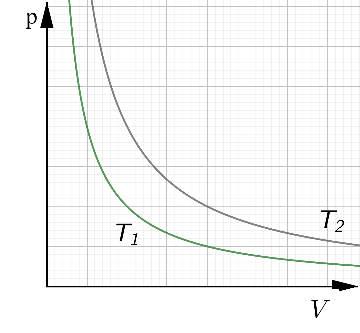
\includegraphics[scale=1.2]{../figs/VN10-2021-PH-TP030-1}
		\end{minipage}
		
	}
	
	\loigiai{\textbf{Đáp án: A.}		
		
		Trong hệ tọa độ (O$pV$), đường đẳng nhiệt ở trên ứng với nhiệt độ cao hơn.
		
	}

		\item \mkstar{1} [29]
	
	\cauhoi{
		Đường biểu diễn sự biến thiên của áp suất theo thể tích khi nhiệt độ không thay đổi gọi là đường đẳng nhiệt. Trong hệ tọa độ (O$pV$) đường đẳng nhiệt có dạng là
		\begin{mcq}
			\item đường thẳng kéo dài đi qua gốc tọa độ O. 
			\item parabol.
			\item hyperbol.
			\item đường thẳng kéo dài song song với trục hoành $\text{O}V$.
		\end{mcq}
	}
	
	\loigiai{\textbf{Đáp án: C.}		
		
		Trong hệ tọa độ (O$pV$) đường đẳng nhiệt có dạng hyperbol.
		
	}

	\item \mkstar{2} [5]
	
	\cauhoi{
		Một lượng khí ở nhiệt độ không đổi $\SI{20}{\celsius}$, thể tích $\SI{2}{m^3}$, áp suất $\SI{2}{atm}$. Nếu áp suất giảm còn $\SI{1}{atm}$ thì thể tích khối khí là bao nhiêu?
		\begin{mcq}(4)
			\item $\SI{4}{m^3}$. 
			\item $\SI{1}{m^3}$.
			\item $\SI{2}{m^3}$.
			\item $\SI{0.5}{m^3}$.
		\end{mcq}
	}
	
	\loigiai{\textbf{Đáp án: A.}		

		Vì nhiệt độ là không đổi nên quá trình là đẳng nhiệt. Áp dụng phương trình:
		$$p_1V_1=p_2V_2 \Rightarrow V_2 = \SI{4}{m^3}.$$
	}
	
	

	\item \mkstar{2} [5]
	
	\cauhoi{
		Một khối khí lí tưởng có thể tích 5 lít, đang ở áp suất $\SI{6}{atm}$ thì dãn nở đẳng nhiệt, áp suất giảm còn $\SI{1.5}{atm}$. Thể tích của khối khí sau khi dãn bằng
		\begin{mcq}(4)
			\item $\SI{20}{l}$.
			\item $\SI{10}{l}$.
			\item $\SI{15}{l}$.
			\item $\SI{1.25}{l}$.
		\end{mcq}
	}
	
	\loigiai{\textbf{Đáp án: A.}		
		
		Vì quá trình là đẳng nhiệt nên ta có phương trình:
		
				$$p_1V_1=v_2V_2 \Rightarrow V_2 = \SI{20}{l}.$$
	}

	

	

	\item \mkstar{2} [29]
	
	\cauhoi{
		Dưới áp suất $p$ một lượng khí có thể tích là 5 lít. Tính thể tích của lượng khí này khi áp suất giảm đi 3 lần so với ban đầu. Biết nhiệt độ được giữ không đổi.
		\begin{mcq}(4)
			\item 15 lít.
			\item 20 lít.
			\item 2,5 lít.
			\item 7,5 lít.
		\end{mcq}
	}
	
	\loigiai{\textbf{Đáp án: A.}		
		
		
		Vì quá trình là đẳng nhiệt nên ta có phương trình:
		
		$$p_1V_1=p_2V_2 \Rightarrow V_2 =\dfrac{p_1}{p_2}V_1 = \dfrac{1}{\dfrac{1}{3}}V_1 = 3V_1= \SI{15}{l}.$$
	}

		\item \mkstar{1} [7]
	
	\cauhoi{
		Phát biểu và viết biểu thức của định luật Bôi-lơ - Ma-ri-ốt (không cần chú thích các đại lượng). Vẽ đường đẳng nhiệt trong hệ tọa độ $\text{O}pV$.
	}
	
	\loigiai{
		Phát biểu:
		\begin{itemize}
			\item Cách 1: Ở nhiệt độ không đổi, tích áp suất và thể tích của một lượng khí lí tưởng xác định là một hằng số;
			\item Cách 2: Trong quá trình đẳng nhiệt của một lượng khí lí tưởng xác định, áp suất tỉ lệ nghịch với thể tích.
		\end{itemize}
		Biểu thức:
		\begin{itemize}
			\item Cách 1: $pV = \text{hằng số}$;
			\item Cách 2: $p_1V_1 = p_2V_2$;
			\item Cách 3: $p\sim \dfrac{1}{V}$.
		\end{itemize}
		Đồ thị:
		
		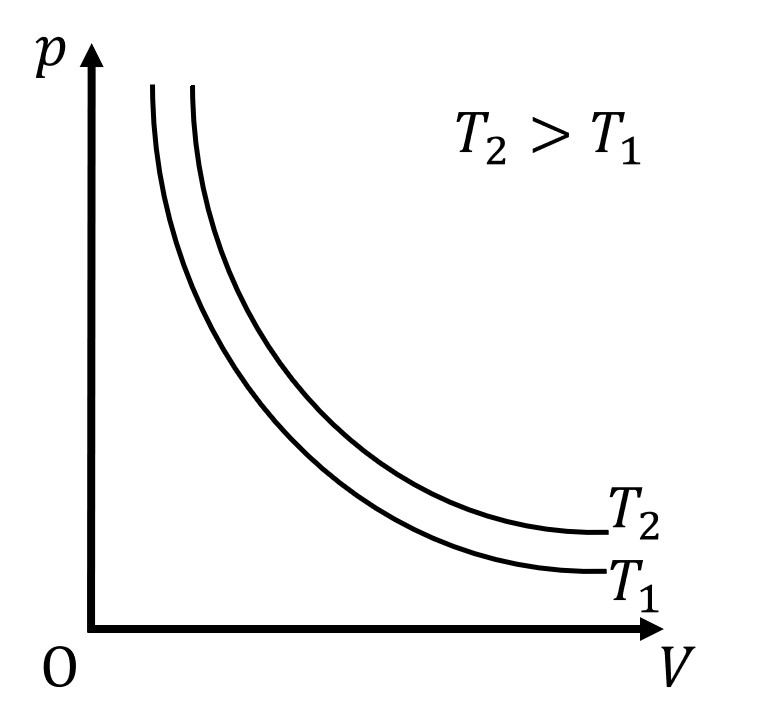
\includegraphics[scale=0.4]{../figs/VN10-PH-37-L-027-1-1-1.jpg}
	}
	
	\item \mkstar{1} [9]
	
	\cauhoi{
		Quá trình đẳng nhiệt là gì?
	}
	
	\loigiai{
		Quá trình đẳng nhiệt là quá trình biến đổi trạng thái mà trong đó nhiệt độ không thay đổi.
	}

	
	\item \mkstar{2} [4]
	
	\cauhoi{
		\begin{enumerate}[label=\alph*)]
			\item Một lượng khí lí tưởng ở trạng thái (1): $p_1=\SI{e5}{Pa}$, $V_1=\SI{30}{l}$. Người ta nén đẳng nhiệt thể tích giảm xuống còn $\SI{20}{l}$. Tính áp suất của chất khí sau khi nén.
			\item Một chất khí lí tưởng ở trạng thái có áp suất $\SI{4e5}{Pa}$, thể tích là $\SI{25}{cm^3}$. Nếu áp suất của chất khí giảm xuống còn $\SI{0.5e5}{Pa}$ thì thể tích khí là bao nhiêu?
		\end{enumerate}
	}
	
	\loigiai{
		\begin{enumerate}[label=\alph*)]
			\item Đẳng nhiệt (1): $p_1=\SI{e5}{Pa}$, $V_1=\SI{30}{l}$ sang (2): $V_2=\SI{20}{l}$, $p_2=?$
			
			Vì quá trình là đẳng nhiệt nên ta có phương trình:
			
			$$p_1V_1=p_2V_2 \Rightarrow p_2 =\dfrac{V_1}{V_2}p_1 = \SI{1.5e5}{Pa}.$$
			
			\item Đẳng nhiệt $p_1=\SI{4e5}{Pa}$, $V_1=\SI{25}{cm^3}$ sang (2): $p_2=\SI{0.5e5}{Pa}$, $V_2=?$
			
			Vì quá trình là đẳng nhiệt nên ta có phương trình:
			
			$$p_1V_1=p_2V_2 \Rightarrow V_2 =\dfrac{p_1}{p_2}V_1 = \SI{200}{cm^3}.$$
			
		\end{enumerate}
	}
	
	
	\item \mkstar{2} [6]
	
	\cauhoi{
		Nghề thợ lặn là một nghề nguy hiểm và yêu cầu phải có sức khỏe cực tốt đặc biệt là khi lặn sâu xuông nước. Cho rằng khi lặn nhiệt độ của nước là không đổi. Bằng kiến thức Vật lý Nhiệt học đã học, em hãy giải thích nguyên nhân dẫn đến nguy hiểm mà người thợ lặn gặp phải.
	}
	
	\loigiai{
		Khi người thợ lặn lặn sâu xuống nước thì áp suất nước tăng ($p$ tăng), mà nhiệt độ của quá trình coi như không đổi, theo định luật Boyle - Mariotte thì $p$ tăng $V$ giảm, khiến phổi người thợ lặn bị co bóp mạnh và gây ra nguy hiểm.
	}

	\item \mkstar{2} [6]
	
	\cauhoi{
		Dưới áp suất $\SI{2e4}{N/m^2}$, một lượng khí có thể tích $\SI{20}{l}$. Tính thể tích của lượng khí đó dưới áp suất $\SI{4e4}{N/m^2}$, coi nhiệt độ không đổi.
	}
	
	\loigiai{
		
		Vì quá trình là đẳng nhiệt nên ta có phương trình:
		
		$$p_1V_1=p_2V_2 \Rightarrow V_2 =\dfrac{p_1}{p_2}V_1 = \SI{10}{l}.$$
	}



	\item \mkstar{2} [11]
	
	\cauhoi{
		Một lượng khí có thể tích $\SI{20}{l}$ và áp suất $\SI{1}{atm}$. Nén đẳng nhiệt khí tới áp suất $\SI{4}{atm}$. Tính thể tích của khí sau khi nén.
	}
	
	\loigiai{
		Đẳng nhiệt (1): $p_1=\SI{1}{atm}$, $V_1=\SI{20}{l}$ sang (2): $V_2=?$, $p_2=\SI{4}{atm}$
		
		Vì quá trình là đẳng nhiệt nên ta có phương trình:
		
		$$p_1V_1=p_2V_2 \Rightarrow V_2 =\dfrac{p_1}{p_2}V_1 = \SI{5}{l}.$$
	}

	\item \mkstar{2} [13]
	
	\cauhoi{
		Một lượng khí trong xi lanh ban đầu có thể tích $V_1=\SI{10}{l}$, nhiệt độ $\SI{227}{\celsius}$, áp suất $p_1=\SI{4}{atm}$ được dãn nở đẳng nhiệt để áp suất giảm 2 lần. Xác định thể tích của lượng khí sau khi nén.
	}
	
	\loigiai{
		
		Đẳng nhiệt (1): $p_1=\SI{4}{atm}$, $V_1=\SI{10}{l}$ sang (2): $V_2=?$, $p_2=\SI{2}{atm}$
		
		Vì quá trình là đẳng nhiệt nên ta có phương trình:
		
		$$p_1V_1=p_2V_2 \Rightarrow V_2 =\dfrac{p_1}{p_2}V_1 = \SI{20}{l}.$$
	}



	\item \mkstar{2} [17]
	
	\cauhoi{
		Một xi-lanh chứa $\SI{150}{cm^3}$ khí ở áp suất $\SI{2e5}{Pa}$. Pit-tông nén khí trong xi-lanh xuống còn $\SI{100}{cm^3}$. Tính áp suất của khí trong xi-lanh lúc này, coi nhiệt độ không đổi.
	}
	
	\loigiai{
		
		Đẳng nhiệt (1): $p_1=\SI{2e5}{Pa}$, $V_1=\SI{150}{cm^3}$ sang (2): $V_2=\SI{100}{cm^3}$, $p_2=?$
		
		Vì quá trình là đẳng nhiệt nên ta có phương trình:
		
		$$p_1V_1=p_2V_2 \Rightarrow p_2 =\dfrac{V_1}{V_2}p_1 = \SI{3e5}{Pa}.$$
	}

	\item \mkstar{2} [18]
	
	\cauhoi{
		Nén khí đẳng nhiệt từ thể tích 18 lít đến thể tích 6 lít thì áp suất tăng thêm một lượng $\Delta p = \SI{60}{kPa}$. Áp suất ban đầu của khí đó là bao nhiêu?
	}
	
	\loigiai{
		
		Đẳng nhiệt (1): $p_1$, $V_1=\SI{18}{l}$ sang (2): $V_2=\SI{6}{l}$, $p_2=p_1+\SI{60}{kPa}$
		
		Vì quá trình là đẳng nhiệt nên ta có phương trình:
		
		$$p_1V_1=p_2V_2 \Rightarrow p_1 = \SI{30}{kPa}.$$
	}

	\item \mkstar{2} [19]
	
	\cauhoi{
		Một khối khí lí tưởng có thể tích $\SI{4}{cm^3}$, áp suất $\SI{8}{atm}$ và nhiệt độ $\SI{27}{\celsius}$. Sau quá trình biến đổi trạng thái người ta thấy nhiệt độ của khối khí không đổi nhưng thể tích của khối khí là $\SI{5}{cm^3}$. Tính áp suất của khối khí sau quá trình biến đổi.
	}
	
	\loigiai{
		
		Đẳng nhiệt (1): $p_1=\SI{8}{atm}$, $V_1=\SI{4}{cm^3}$ sang (2): $V_2=\SI{5}{cm^3}$, $p_2=?$
		
		Vì quá trình là đẳng nhiệt nên ta có phương trình:
		
		$$p_1V_1=p_2V_2 \Rightarrow p_2 =\dfrac{V_1}{V_2}p_1 = \SI{6.4}{atm}.$$
	}

	\item \mkstar{2} [19]
	
	\cauhoi{
		Một khối khí được nén từ thể tích 16 lít xuống còn 8 lít, khi đó áp suất của khí tăng thêm $\SI{0.5}{atm}$. Tìm áp suất ban đầu của khí biết trong quá trình nén, nhiệt độ được giữ không đổi.
	}
	
	\loigiai{
		Đẳng nhiệt (1): $p_1$, $V_1=\SI{16}{l}$ sang (2): $V_2=\SI{8}{l}$, $p_2=p_1+\SI{0.5}{atm}$
		
		Vì quá trình là đẳng nhiệt nên ta có phương trình:
		
		$$p_1V_1=p_2V_2 \Rightarrow p_1 = \SI{0.5}{atm}.$$
	}

	\item \mkstar{2} [28]
	
	\cauhoi{
		Một lượng khí được nén đẳng nhiệt từ thể tích 10 lít còn 4 lít, khi đó áp suất tăng thêm $\SI{1.5}{atm}$. Áp suất khí ban đầu là bao nhiêu?
	}
	
	\loigiai{
		Đẳng nhiệt (1): $p_1$, $V_1=\SI{10}{l}$ sang (2): $V_2=\SI{4}{l}$, $p_2=p_1+\SI{1.5}{atm}$
		
		Vì quá trình là đẳng nhiệt nên ta có phương trình:
		
		$$p_1V_1=p_2V_2 \Rightarrow p_1 = \SI{1}{atm}.$$
	}


	\item \mkstar{2} [31]
	
	\cauhoi{
		Khi có thể tích 5 lít, áp suất $\SI{2}{atm}$. Giữ nhiệt độ khí không đổi và giảm thể tích xuống còn 2 lít. Tính áp suất khí lúc này.
	}
	
	\loigiai{
		Đẳng nhiệt (1): $p_1=\SI{2}{atm}$, $V_1=\SI{5}{l}$ sang (2): $V_2=\SI{2}{l}$, $p_2=?$
		
		Vì quá trình là đẳng nhiệt nên ta có phương trình:
		
		$$p_1V_1=p_2V_2 \Rightarrow p_2 =\dfrac{V_1}{V_2}p_1 = \SI{5}{atm}.$$
		
	}

	\item \mkstar{2} [32]
	
	\cauhoi{
		Quan sát người thợ lặn dưới một hồ nước người ta nhận thấy các bọt khí tạo ra càng lúc càng to lên khi tiến gần đến mặt nước. Em hãy dùng định luật Boyle Mariotte để giải thích hiện tượng trên. Xem nhiệt độ của nước là như nhau tại mọi nơi trong hồ nước.
	}
	
	\loigiai{
		Do quá trình là đẳng nhiệt, áp suất tỉ lệ nghịch với thể tích khí. Càng gần mặt nước thì áp suất càng giảm, do đó thể tích càng tăng, nên bong bóng càng to ra.
		
	}
	\item \mkstar{3} [15]

\cauhoi{
	Người ta bơm khí vào một quả bóng có dung tích $\SI{3}{l}$. Mỗi lần bơm được $\SI{300}{cm^3}$ khí ở áp suất $\SI{1}{atm}$ vào bên trong quả bóng. Vỏ bóng chịu được áp suất tối đa là $\SI{2.5}{atm}$. Sau 20 lần bơm, quả bóng có bị nổ không? Tại sao? Cho rằng nhiệt độ không thay đổi trong suốt quá trình bơm và trước khi bơm trong quả bóng không có không khí.
}

\loigiai{
	Đổi $\Delta V = \SI{300}{cm^3} = \SI{0.3}{l}$.
	
	Sau 20 lần bơm thì $\Delta V_{20} = 20\Delta V = \SI{6}{l}$.
	
	Xem quá trình như là đẳng nhiệt nén lượng không khí từ bên ngoài (20 lần bơm) nén vào trong 1 quả bóng có thể tích 3 lít: (1): $p_1=\SI{1}{atm}$, $V_1=\SI{6}{l}$ sang (2): $V_2=\SI{3}{l}$, $p_2=?$
	
	Vì quá trình là đẳng nhiệt nên ta có phương trình:
	
	$$p_1V_1=p_2V_2 \Rightarrow p_2 =\dfrac{V_1}{V_2}p_1 = \SI{2}{atm}.$$
	
	Quả bóng chịu được áp suất tối đa là $\SI{2.5}{atm}$ nên không phát nổ.
}

\item \mkstar{3} [29]

\cauhoi{
	Nén khí đẳng nhiệt từ thể tích 6 lít đến thể tích 9 lít thì áp suất thay đổi một lượng bằng $\SI{2.5}{atm}$. Tính áp suất ban đầu của khối khí này.
}

\loigiai{
	Vì áp suất tỉ lệ nghịch với thể tích nên thể tích tăng thì áp suất giảm, dẫn đến $p_2=p_1-\Delta p$.
	
	Quá trình đẳng nhiệt (1): $p_1$, $V_1=\SI{6}{l}$ sang (2): $V_2=\SI{9}{l}$, $p_2=p_1-\SI{2.5}{atm}$
	
	Vì quá trình là đẳng nhiệt nên ta có phương trình:
	
	$$p_1V_1=p_2V_2 \Rightarrow p_1 = \SI{7.5}{atm}.$$
}
\end{enumerate}
\whiteBGstarEnd
	\stopcontents[mychapters]
	
	\setcounter{mychapter}{29}
	\mychapter[Quá trình đẳng tích. Định luật Sác-lơ]{Quá trình đẳng tích.\\ Định luật Sác-lơ}
	\startcontents[mychapters]
	\printcontents[mychapters]{}{0}{\setcounter{tocdepth}{1}}
	\whiteBGstarBegin
\setcounter{section}{0}
\begin{enumerate}[label=\bfseries Câu \arabic*:]
	
	\item \mkstar{1} [4]
	
	\cauhoi{
		Hệ thức nào sau đây phù hợp với định luật Sác-lơ?
		\begin{mcq}(4)
			\item $p\sim t$.
			\item $\dfrac{p_1}{T_1} = \dfrac{p_2}{T_2}$.
			\item $\dfrac{p}{t} = \text{hằng số}$.
			\item $\dfrac{p_1}{p_2} = \dfrac{T_2}{T_1}$.
		\end{mcq}
	}
	
	\loigiai{
		\textbf{Đáp án: B.}
		
		Hệ thức phù hợp với định luật Sác-lơ là $\dfrac{p}{T} = \text{hằng số}$, hoặc $\dfrac{p_1}{T_1} = \dfrac{p_2}{T_2}$, với $T$ viết in hoa chỉ nhiệt độ tuyệt đối.
	}
	
	\item \mkstar{1} [5]
	
	\cauhoi{
		Quá trình biến đổi trạng thái trong đó thể tích được giữ không đổi gọi là quá trình
		\begin{mcq}(4)
			\item đẳng nhiệt. 
			\item đẳng áp.
			\item đoạn nhiệt.
			\item đẳng tích.
		\end{mcq}
		
	}
	
	\loigiai{
		\textbf{Đáp án: D.}
		
		Quá trình biến đổi trạng thái trong đó thể tích được giữ không đổi gọi là quá trình đẳng tích.
	}

		\item \mkstar{1} [5]

\cauhoi{
	Trong các hệ thức sau, hệ thức nào \textbf{không} phù hợp với quá trình đẳng tích?
	\begin{mcq}(4)
		\item $p\sim t$. 
		\item $p\sim T$.
		\item $\dfrac{p_1}{T_1} = \dfrac{p_2}{T_2}$.
		\item $\dfrac{p}{T} = \text{hằng số}$.
	\end{mcq}
	
}

\loigiai{
	\textbf{Đáp án: A.}
	
	Hệ thức phù hợp với định luật Sác-lơ là $\dfrac{p}{T} = \text{hằng số}$, hoặc $\dfrac{p_1}{T_1} = \dfrac{p_2}{T_2}$, với $T$ viết in hoa chỉ nhiệt độ tuyệt đối.
	
	Vậy $p\sim t$ không phù hợp với quá trình đẳng tích.
}
		\item \mkstar{1} [24]

\cauhoi{
	Quá trình đẳng tích là quá trình biến đổi trạng thái trong đó
	\begin{mcq}(2)
		\item nhiệt độ được giữ không đổi. 
		\item áp suất được giữ không đổi.
		\item lực nén được giữ không đổi.
		\item thể tích được giữ không đổi.
	\end{mcq}
	
}

\loigiai{
	\textbf{Đáp án: D.}
	
	Quá trình đẳng tích là quá trình biến đổi trạng thái trong đó thể tích được giữ không đổi.
}
		\item \mkstar{1} [32]

\cauhoi{
	Trong hệ tọa độ ($p,T$) đường biểu diễn nào sau đây là đường đẳng tích?
	\begin{mcq}
		\item Đường hyperbol.
		\item Đường thẳng kéo dài đi qua gốc tọa độ.
		\item Đường thẳng kéo dài không đi qua gốc tọa độ.
		\item Đường thẳng cắt trục $p$ tại điểm $p=p_0$.
	\end{mcq}
	
}

\loigiai{
	\textbf{Đáp án: B.}
	
	Trong hệ tọa độ ($p,T$) đường đẳng tích là đường thẳng kéo dài đi qua gốc tọa độ.
}
		\item \mkstar{2} [5]
	
	\cauhoi{
		Một khối khí lí tưởng đang ở nhiệt độ $\SI{37}{\celsius}$, áp suất $\SI{4}{atm}$ thì được làm lạnh đẳng tích cho đến khi áp suất còn $\SI{2}{atm}$. Nhiệt độ của khối khí lúc đó bằng
		\begin{mcq}(4)
			\item $\SI{-118}{\celsius}$. 
			\item $\SI{775}{\celsius}$.
			\item $\SI{155}{\celsius}$.
			\item $\SI{129}{\celsius}$.
		\end{mcq}
		
	}
	
	\loigiai{
		\textbf{Đáp án: A.}
		
		Đẳng tích (1): $p_1=\SI{4}{atm}$, $T_1=\SI{310}{K}$ sang (2): $p_2=\SI{2}{atm}$, $T_2=?$
		
		Vì quá trình là đẳng tích nên ta có phương trình:
		
		$$\dfrac{p_1}{T_1} = \dfrac{p_2}{T_2} \Rightarrow T_2 =\dfrac{T_1p_2}{p_1} = \SI{155}{K}.$$
		
		Đổi $t_2 = T_2 - 273 = \SI{-118}{\celsius}$.
	}



		\item \mkstar{2} [5]
	
	\cauhoi{
		Một lốp ô tô chứa không khí ở áp suất $\SI{5}{bar}$, nhiệt độ $\SI{25}{\celsius}$. Khi xe chạy, nhiệt độ trong lốp tăng lên đến $\SI{50}{\celsius}$, áp suất không khí trong lốp khi đó là
		\begin{mcq}(4)
			\item $\SI{10.45}{bar}$. 
			\item $\SI{10}{bar}$.
			\item $\SI{5.42}{bar}$.
			\item $\SI{4.55}{bar}$.
		\end{mcq}
		
	}
	
	\loigiai{
		\textbf{Đáp án: C.}
		
			Đẳng tích (1): $p_1=\SI{5}{bar}$, $T_1=\SI{298}{K}$ sang (2): $p_2=?$, $T_2=\SI{323}{K}$
		
		Vì quá trình là đẳng tích nên ta có phương trình:
		
		$$\dfrac{p_1}{T_1} = \dfrac{p_2}{T_2} \Rightarrow p_2 =\dfrac{p_1T_2}{T_1} = \SI{5.42}{bar}.$$
	}



		\item \mkstar{2} [24]
	
	\cauhoi{
		Quá trình nào sau đây có thể xem là quá trình đẳng tích?
		\begin{mcq}
			\item Thổi không khí vào một quả bóng bay. 
			\item Đun nóng khí trong một xi lanh có pit-tông cố định.
			\item Đun nóng khí trong một xi lanh có pit-tông không cố định.
			\item Quả bóng bàn bị bẹp nhúng vào nước nóng, phồng lên như cũ.
		\end{mcq}
		
	}
	
	\loigiai{
		\textbf{Đáp án: B.}
		
		Đun nóng khí trong một xi lanh có pit-tông cố định thì thể tích khí bên trong không đổi, do đó có thể xem là quá trình đẳng tích.
	}

		\item \mkstar{2} [24]
	
	\cauhoi{
		Một khối khí lí tưởng được đựng trong bình kín. Sau khi khối khí được đun nóng, nhiệt độ tuyệt đối của khối khí là $\SI{360}{K}$ và áp suất của khối khí tăng gấp 1,2 lần. Nhiệt độ tuyệt đối ban đầu của khối khí là
		\begin{mcq}(4)
			\item $\SI{60}{K}$. 
			\item $\SI{72}{K}$.
			\item $\SI{300}{K}$.
			\item $\SI{360}{K}$.
		\end{mcq}
		
	}
	
	\loigiai{
		\textbf{Đáp án: C.}
		
		Đẳng tích (1): $p_1$, $T_1=?$ sang (2): $p_2=1,2p_1$, $T_2=\SI{360}{K}$
		
		Vì quá trình là đẳng tích nên ta có phương trình:
		
		$$\dfrac{p_1}{T_1} = \dfrac{p_2}{T_2} \Rightarrow T_1 =\dfrac{p_1T_2}{p_2} = \SI{300}{bar}.$$
	}

		\item \mkstar{2} [29]
	
	\cauhoi{
		Ở điều kiện tiêu chuẩn, chất khí ở $\SI{0}{C}$ có áp suất $\SI{1}{atm}$. Coi thể tích của chất khí là không đổi, áp suất khí ở $\SI{47}{\celsius}$ có giá trị xấp xỉ bằng
		\begin{mcq}(4)
			\item $\SI{1.17}{atm}$. 
			\item $\SI{1.56}{atm}$.
			\item $\SI{1.92}{atm}$.
			\item $\SI{1.25}{atm}$.
		\end{mcq}
		
	}
	
	\loigiai{
		\textbf{Đáp án: A.}
		
		Đẳng tích (1): $p_1=\SI{1}{atm}$, $T_1=\SI{273}{K}$ sang (2): $p_2=?$, $T_2=\SI{320}{K}$
		
		Vì quá trình là đẳng tích nên ta có phương trình:
		
		$$\dfrac{p_1}{T_1} = \dfrac{p_2}{T_2} \Rightarrow p_2 =\dfrac{p_1T_2}{T_1} = \SI{1.17}{atm}.$$
	}


	
	\item \mkstar{1} [2]
	
	\cauhoi{
		Quá trình đẳng tích là gì? Phát biểu và viết công thức định luật liên quan. Vẽ đường đẳng tích trong hệ trục ($p,T$) với $\text{O}T$ là trục hoành.
	}
	
	\loigiai{		
		Quá trình biến đổi trạng thái mà trong đó thể tích được giữ không đổi gọi là quá trình đẳng tích.
		
		Trong quá trình đẳng tích, áp suất tỉ lệ thuận với nhiệt độ tuyệt đối.
		
		Công thức định luật Sác-lơ: $p\sim T$ hay $\dfrac{p}{T} = \text{hằng số}$ hay $\dfrac{p_1}{T_1}=\dfrac{p_2}{T_2}$.
		
		Đường đẳng tích trong hệ trục ($p,T$) với $\text{O}T$ là trục hoành:
		\begin{center}
			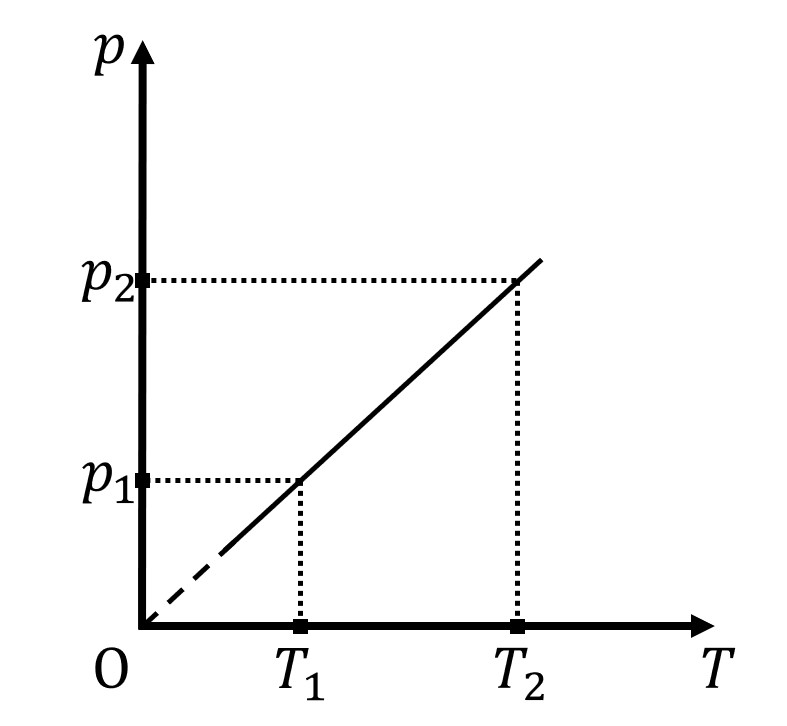
\includegraphics[scale=0.4]{../figs/VN10-PH-39-L-0293-4.jpg}
		\end{center}
	}
	
	
	\item \mkstar{2} [3]
	
	\cauhoi{
		Xét lượng khí xác định chứa trong bình kín có thể tích $V$ không đổi. Khi tăng nhiệt độ tuyệt đối thì áp suất của lượng khí thay đổi như thế nào (tăng hay giảm)? Giải thích.
	}
	
	\loigiai{
		Trong quá trình đẳng tích, áp suất tỉ lệ thuận với nhiệt độ tuyệt đối. Vậy khi tăng nhiệt độ tuyệt đối thì áp suất của lượng khí tăng.
	}
	
	\item \mkstar{2} [7]
	
	\cauhoi{
		Một lượng khí hidro đựng trong bình kín có thể tích không đổi. Ở áp suất $\SI{1.5}{atm}$ thì nhiệt độ của khối khí là $\SI{27}{\celsius}$.
		\begin{enumerate}[label=\alph*)]
			\item Tính áp suất của khí khi đun nóng đến $\SI{127}{\celsius}$.
			\item Để áp suất của khí là $\SI{3}{atm}$ thì phải đun nóng đến bao nhiêu độ C?
		\end{enumerate}
	}
	
	\loigiai{
		\begin{enumerate}[label=\alph*)]
			\item Tính áp suất của khí khi đun nóng đến $\SI{127}{\celsius}$.
			
			Đẳng tích (1): $p_1=\SI{1.5}{atm}$, $T_1=\SI{300}{K}$ sang (2): $p_2=?$, $T_2=\SI{400}{K}$
			
			Vì quá trình là đẳng tích nên ta có phương trình:
			
			$$\dfrac{p_1}{T_1} = \dfrac{p_2}{T_2} \Rightarrow p_2 =\dfrac{p_1T_2}{T_1} = \SI{2}{atm}.$$
			
			\item Để áp suất của khí là $\SI{3}{atm}$ thì phải đun nóng đến bao nhiêu độ C?.
			
			Đẳng tích (1): $p_1=\SI{1.5}{atm}$, $T_1=\SI{300}{K}$ sang (2): $p_2=\SI{3}{atm}$, $T_2=?$
			
			Vì quá trình là đẳng tích nên ta có phương trình:
			
			$$\dfrac{p_1}{T_1} = \dfrac{p_2}{T_2} \Rightarrow T_2 =\dfrac{p_2T_1}{p_1} = \SI{600}{K}.$$
			
			Đổi $t_2=T_2-273 = \SI{327}{\celsius}$.
		\end{enumerate}
		
	}

	\item \mkstar{2} [8]
	
	\cauhoi{
		Tại sao lốp xe ô tô thường nổ khi xe đang chạy ngoài trời nóng hơn là để xe nằm yên trong gara? Định luật vật lý nào mà em đã học có thể giải thích hiện tượng trên?
	}
	
	\loigiai{
		Khi lốp xe đang chạy trên đường, do ma sát với đường và nắng nóng làm cho nhiệt độ của không khí bên trong lốp xe tăng lên, làm cho áp suất khí trong lốp xe tăng lên theo (quá trình đẳng tích). Khi áp suất tăng đến một mức nào đó thì có thể gây nổ lốp xe.
		
		Khi để xe trong gara, do nhiệt độ không cao như trường hợp trên nên áp suất khối khí cũng không cao, lốp xe khó nổ hơn.
		
		Giải thích hiện tượng trên, ta dùng định định luật Sác-lơ về quá trình đẳng tích.
		
	}
	\item \mkstar{2} [11]

\cauhoi{
	
	Đun nóng đẳng tích lượng khí lí tưởng từ nhiệt độ tuyệt đối $\SI{150}{K}$, áp suất $\SI{4}{atm}$. Tìm nhiệt độ tuyệt đối của khối khí khi áp suất là $\SI{6}{atm}$.
}

\loigiai{
	Đẳng tích (1): $p_1=\SI{4}{atm}$, $T_1=\SI{150}{K}$ sang (2): $p_2=\SI{6}{atm}$, $T_2=?$
	
	Vì quá trình là đẳng tích nên ta có phương trình:
	
	$$\dfrac{p_1}{T_1} = \dfrac{p_2}{T_2} \Rightarrow T_2 =\dfrac{p_2T_1}{p_1} = \SI{225}{K}.$$
	
}

\item \mkstar{2} [12]

\cauhoi{
	
	Các quả bóng bay là món đồ chơi được trẻ em thích nhưng khí được bơm vào bóng bay thường là hydro, metan hoặc khí đất đèn rất nguy hiểm khi cháy nổ. Hãy giải thích tại sao bóng bay để ngoài trời nắng nóng lại phát nổ?
}

\loigiai{
	
	Khi để ngoài trời nắng nóng thì nhiệt độ tăng, làm cho áp suất khí bên trong quả bóng tăng. Khi áp suất tăng vượt quá giới hạn mà vỏ quả bóng chịu được thì quả bóng phát nổ. Hiện tượng này được giải thích bằng định luật Sác-lơ cho quá trình đẳng tích.
	
}

\item \mkstar{2} [18]

\cauhoi{
	
	Một bóng đèn dây tóc chứa khí trơ, khi đèn sáng nhiệt độ của bóng đèn là $\SI{450}{\celsius}$, áp suất khí trong bóng đèn bằng áp suất khí quyển là $\SI{1}{atm}$. Tính áp suất khí trong bóng đèn khi đèn chưa sáng ở $\SI{22}{\celsius}$.
}

\loigiai{
	Đẳng tích (1): $p_1=\SI{1}{atm}$, $T_1=\SI{723}{K}$ sang (2): $p_2=?$, $T_2=\SI{295}{K}$
	
	Vì quá trình là đẳng tích nên ta có phương trình:
	
	$$\dfrac{p_1}{T_1} = \dfrac{p_2}{T_2} \Rightarrow p_2 =\dfrac{p_1T_2}{T_1} = \SI{1.17}{atm}.$$
	
}

\item \mkstar{2} [22]

\cauhoi{
	
	Vì sao nồi áp suất có thể nấu chín thịt trong một thời gian ngắn?
}

\loigiai{
	Do nồi áp suất có kết cấu kín (thể tích khí bên trong không đổi), khi ở $\SI{100}{\celsius}$, các phân tử hơi nước không thoát được ra ngoài, khí này sẽ bị giữ lại trong nồi ngày càng nhiều, làm cho áp suất không khí trong nồi tăng cao. Khi áp suất tăng dẫn đến điểm sôi (nhiệt độ mà tại đó có sự sôi xảy ra) cũng tăng, nước không thể bị hóa hơi mà buộc phải hấp thụ nhiệt lượng tiếp tục tăng nhiệt độ, luôn giữ ở trạng thái sôi. Trong quá trình này nhiệt lượng được thức ăn hấp thu ngày càng nhiều. Nhiệt độ trong nồi áp suất có thể đạt tới $\SI{120}{\celsius}$, ở nhiệt độ này, thức ăn rất mau chín.
	
}
\item \mkstar{2} [30]

\cauhoi{
	
	\begin{enumerate}[label=\alph*)]
		\item Đẳng quá trình là quá trình biến đổi trạng thái mà trong đó có một thông số không thay đổi. Dựa vào đó, em hãy cho biết thế nào là quá trình đẳng tích?
		\item Trong quá trình đẳng tích, áp suất và nhiệt độ tuyệt đối có mối quan hệ như thế nào?
		\item Một săm xe máy được bơm căng không khí ở nhiệt độ $\SI{20}{\celsius}$ và áp suất $\SI{2}{atm}$. Tính áp suất trong săm xe khi nhiệt độ lên đến $\SI{42}{\celsius}$. Từ đó cho biết săm có bị nổ không nếu coi như sự tăng thể tích của săm là không đáng kể và săm chịu được áp suất tối đa là $\SI{2.5}{atm}$.
	\end{enumerate}
}

\loigiai{
	\begin{enumerate}[label=\alph*)]
		\item Quá trình đẳng tích là quá trình biến đổi trạng thái mà trong đó thể tích không thay đổi.
		\item Trong quá trình đẳng tích, áp suất tỉ lệ thuận với nhiệt độ tuyệt đối.
		\item Đẳng tích (1): $p_1=\SI{2}{atm}$, $T_1=\SI{293}{K}$ sang (2): $p_2=?$, $T_2=\SI{315}{K}$
		
		Vì quá trình là đẳng tích nên ta có phương trình:
		
		$$\dfrac{p_1}{T_1} = \dfrac{p_2}{T_2} \Rightarrow p_2=\dfrac{p_1T_2}{T_1} = \SI{2.15}{atm}.$$
		
		Vì $\SI{2.15}{atm} < \SI{2.5}{atm}$ nên săm không bị nổ.
	\end{enumerate}
	
}
	\item \mkstar{3} [10]
	
	\cauhoi{
		
		Đun nóng đẳng tích một khối khí lên thêm $\SI{10}{\celsius}$ thì áp suất tăng thêm $1/50$ áp suất khí ban đầu. Tìm nhiệt độ ban đầu của khí.
	}
	
	\loigiai{
		Đẳng tích (1): $p_1$, $T_1$ sang (2): $p_2=(1+1/50)p_1$, $T_2=T_1+10$
		
		Vì quá trình là đẳng tích nên ta có phương trình:
		
		$$\dfrac{p_1}{T_1} = \dfrac{p_2}{T_2} \Rightarrow T_1 =\dfrac{p_1T_2}{p_2} = \SI{500}{K}.$$
		
		Đổi $t_1=T_1 - 273 = \SI{227}{\celsius}$.
		
	}



	\item \mkstar{3} [27]
	
	\cauhoi{
		PSI là chỉ số áp suất của không khí bị nén trong lốp xe, được đo bằng đơn vị Pounds trên một Inch vuông (Pounds per Square Inch). PSI thường được ghi trên thành lốp xe, nó cho biết áp suất tối đa mà lốp xe chịu được. Khi bơm hoặc khi kiểm tra lốp, chúng ta phải làm sao cho lớp đủ hơi, tức là có đủ số PSI cần thiết, thiếu quá hoặc thừa quá đều có thể đưa đến tình trạng hại xe, hư lốp, hao mòn và nguy hiểm nhất là nổ lốp, gây ra tai nạn trầm trọng.
			
			Một chiếc lốp sau của xe Vinfast chứa không khí ở áp suất $\SI{40}{PSI}$ (đổi đơn vị $\SI{1}{PSI} \approx \SI{6895}{Pa}$) và nhiệt độ $\SI{27}{\celsius}$. Khi xe chạy nhanh, lốp xe nóng lên làm nhiệt độ không khí trong lốp xe tăng tới $\SI{57}{\celsius}$. Chỉ số PSI an toàn ghi trên lốp xe của dòng xe này là $\SI{46}{PSI}$. Bỏ qua sự dãn nở của lốp xe, hỏi lốp xe có bị nổ không? Vì sao?
		
	
	}
	
	\loigiai{
	
		Đẳng tích (1): $p_1=\SI{40}{PSI}$, $T_1=\SI{300}{K}$ sang (2): $p_2=?$, $T_2=\SI{330}{K}$
		
		Vì quá trình là đẳng tích nên ta có phương trình:
		
		$$\dfrac{p_1}{T_1} = \dfrac{p_2}{T_2} \Rightarrow p_2 =\dfrac{p_1T_2}{T_1} = \SI{44}{PSI}.$$
		
		Vì $\SI{44}{PSI} < \SI{46}{PSI}$ nên lốp xe không bị nổ.
		
	}

	\item \mkstar{3} [28]
	
	\cauhoi{
		Để giảm thiểu thời gian đi lại, vận chuyển sản phẩm giao thương giữa các vùng miền tổ quốc, Việt Nam đã có chủ trương tiến hành xây dựng tuyến đường cao tốc Bắc - Nam với tốc độ tối đa rất cao từ $\SI{80}{km/h} \rightarrow \SI{120}{km/h}$. Đường cao tốc của Việt Nam được xây dựng theo đúng tiêu chuẩn quốc tế, do đó mặt đường sẽ có độ nhám rất cao. Độ bám và ma sát của bánh xe với mặt đường tăng lên giúp hạn chế nguy cơ xảy ra tai nạn nhưng lại khiến lốp xe nhanh bị mài mòn hơn.
		\begin{enumerate}[label=\alph*)]
			\item Nếu em là tài xế chạy trên đường cao tốc, em hãy giải thích tại sao ô tô thường nổ lốp trên đường cao tốc và gây ra rất nhiều tai nạn thương tâm? Nêu biện pháp khắc phục để giảm thiểu tình trạng trên.
			\item Giả sử có một lốp ô tô chịu được áp suất tối đa $\SI{40}{kPa}$. Lốp được bơm đầy không khí ở nhiệt độ $\SI{27}{\celsius}$ với áp suất $\SI{36}{kPa}$. Khi chạy trên đường cao tốc, lốp xe nóng lên tới $\SI{67}{\celsius}$ thì có bị nổ không? Vì sao? (Bỏ qua sự nở vì nhiệt của lốp xe).
		\end{enumerate}
	}
	
	\loigiai{
		\begin{enumerate}[label=\alph*)]
			\item Khi di chuyển trên đường cao tốc, xe chạy với tốc độ càng nhanh thì lốp càng nóng. Điều này khiến áp suất của lốp tăng nhanh làm cho lốp dễ bị nổ. Giải thích hiện tượng trên dựa vào định luật Sác-lơ cho quá trình đẳng tích.
			
			\item Đẳng tích (1): $p_1=\SI{36}{kPa}$, $T_1=\SI{300}{K}$ sang (2): $p_2=?$, $T_2=\SI{340}{K}$
			
			Vì quá trình là đẳng tích nên ta có phương trình:
			
			$$\dfrac{p_1}{T_1} = \dfrac{p_2}{T_2} \Rightarrow p_2 =\dfrac{p_1T_2}{T_1} = \SI{40.8}{kPa}.$$
			
			Vì $\SI{40.8}{kPa} > \SI{40}{kPa}$ nên lốp xe bị nổ.
		\end{enumerate}
		
	}

\item \mkstar{3} [30]

\cauhoi{
	
	\begin{enumerate}[label=\alph*)]
		\item Trong các buối hội chợ, gian hàng ẩm thực các ngày trại truyền thống, trại xuân của trường học, các học sinh thường sử dụng bếp gas mini để nấu nướng. Tuy nhiên cũng vì lí do đó mà xảy ra một số tai nạn liên quan đến nổ bình gas, bếp gas do sử dụng dưới trời nắng nóng. Dựa vào kiến thức đã học, em hãy giải thích tại sao khi để bình gas dưới nắng nóng thì rất dễ bị phát nổ?
		\item Vận dụng: một bình gas mini kín có ghi thông số áp suất tối đa mà vỏ bình chịu được là $\SI{6.5}{kgf/cm^2}$. Nếu đem ra ngoài nắng làm cho nhiệt độ của khối khí trong bình tăng 1,5 lần thì áp suất tăng $\SI{2.5}{kgf/cm^2}$. Bình gas trên có phát nổ không? Coi khí gas trong bình là khí lí tưởng.
	\end{enumerate}
}

\loigiai{
	\begin{enumerate}[label=\alph*)]
		\item Khi để bình gas dưới nắng nóng thì nhiệt độ tăng cao làm cho áp suất khí gas tăng cao. Khi tăng đến một lúc nào đó vượt giới hạn chịu đựng của vỏ bình thì bình gas phát nổ. Giải thích hiện tượng trên dựa vào định luật Sác-lơ cho quá trình đẳng tích.
		
		\item Đẳng tích (1): $p_1$, $T_1$ sang (2): $p_2=p_1+\SI{2.5}{kgf/cm^2}$, $T_2=1,5T_1$
		
		Vì quá trình là đẳng tích nên ta có phương trình:
		
		$$\dfrac{p_1}{T_1} = \dfrac{p_2}{T_2} \Rightarrow p_2=p_1+2,5 =\dfrac{p_1T_2}{T_1} \Rightarrow p_1= \SI{5}{kgf/cm^2} \Rightarrow p_2 = \SI{7.5}{kgf/cm^2}.$$
		
		Vì $\SI{7.5}{kgf/cm^2} > \SI{6.5}{kgf/cm^2}$ nên bình gas mini bị nổ.
	\end{enumerate}
	
}


\end{enumerate}
\whiteBGstarEnd
	\stopcontents[mychapters]
	
	\setcounter{mychapter}{30}
	\mychapter[Phương trình trạng thái của khí lí tưởng]{Phương trình trạng thái\\ của khí lí tưởng}
	\startcontents[mychapters]
	\printcontents[mychapters]{}{0}{\setcounter{tocdepth}{1}}
	\whiteBGstarBegin
\setcounter{section}{0}
\section{Lý thuyết: Quá trình đẳng áp}
\begin{enumerate}[label=\bfseries Câu \arabic*:]
	
	\item \mkstar{1} [5]
	
	\cauhoi{
		Hệ thức nào sau đây \textbf{không} phù hợp với quá trình đẳng áp?
		\begin{mcq}(4)
			\item $V\sim \dfrac{1}{T}$.
			\item $\dfrac{V}{T} = \text{hằng số}$.
			\item $\dfrac{V_1}{T_1} = \dfrac{V_2}{T_2}$.
			\item $V\sim T$.
		\end{mcq}
	}
	
	\loigiai{
		\textbf{Đáp án: A.}
		
		Hệ thức phù hợp với quá trình đẳng áp là $V\sim T$ hay $\dfrac{V}{T} = \text{hằng số}$ hay $\dfrac{V_1}{T_1}=\dfrac{V_2}{T_2}$.
	}

\item \mkstar{1} [5]

\cauhoi{
	Quá trình biến đổi trạng thái trong đó áp suất được giữ không đổi gọi là quá trình
	\begin{mcq}(4)
		\item đẳng tích.
		\item đẳng áp.
		\item đẳng nhiệt.
		\item đoạn nhiệt.
	\end{mcq}
}

\loigiai{
	\textbf{Đáp án: B.}
	
	Quá trình biến đổi trạng thái trong đó áp suất được giữ không đổi gọi là quá trình đẳng áp.
}
	\item \mkstar{1} [24]

\cauhoi{
	Trong quá trình đẳng áp, thông số trạng thái nào thay đổi?
	\begin{mcq}(2)
		\item Nhiệt độ và áp suất. 
		\item Nhiệt độ và thể tích.
		\item Thể tích và áp suất.
		\item Nhiệt độ, áp suất và thể tích.
	\end{mcq}
	
}

\loigiai{
	\textbf{Đáp án: B.}
	
	Trong quá trình đẳng áp, áp suất được giữ không đổi, nhiệt độ và thể tích thay đổi.
}
\item \mkstar{1} [24]

\cauhoi{
	Phương trình nào sau đây là phương trình trạng thái khí lí tưởng?
	\begin{mcq}(2)
		\item $\dfrac{VT}{p} = \text{hằng số}$. 
		\item $\dfrac{p_1V_2}{T_1} = \dfrac{p_2V_1}{T_2} = \text{hằng số}$.
		\item $\dfrac{pT}{V} = \text{hằng số}$.
		\item $\dfrac{pV}{T} = \text{hằng số}$.
	\end{mcq}
}

\loigiai{
	\textbf{Đáp án: D.}
	
	Phương trình trạng thái khí lí tưởng: $\dfrac{pV}{T} = \text{hằng số}$ hoặc $\dfrac{p_1V_1}{T_1} = \dfrac{p_2V_2}{T_2}$.
}

\item \mkstar{2} [5]

\cauhoi{
	Một khối khí có áp suất không đổi ở nhiệt độ $\SI{50}{\celsius}$. Nhiệt độ khối khí phải tăng đến bao nhiêu để thể tích tăng gấp đôi?
	\begin{mcq}(4)
		\item $\SI{200}{\celsius}$.
		\item $\SI{100}{\celsius}$.
		\item $\SI{373}{\celsius}$.
		\item $\SI{646}{\celsius}$.
	\end{mcq}
}

\loigiai{
	\textbf{Đáp án: ABC.}
	
	Đẳng áp (1): $V_1$, $T_1=\SI{323}{K}$ sang (2): $V_2=2V_1$, $T_2=?$
	
	Vì quá trình là đẳng áp nên ta có phương trình:
	
	$$\dfrac{V_1}{T_1} = \dfrac{V_2}{T_2} \Rightarrow T_2 =\dfrac{V_2T_1}{V_1} = \SI{646}{K}.$$
	
	Đổi $t_2=T_2-273 = \SI{373}{\celsius}$.
}

\item \mkstar{2} [5]

\cauhoi{
	Giữ áp suất của một khối lượng khí không thay đổi, để thể tích tăng lên gấp 3 lần thì nhiệt độ tuyệt đối
	\begin{mcq}(2)
		\item tăng lên 3 lần.
		\item giảm đi 3 lần.
		\item tăng lên 6 lần.
		\item giảm đi 6 lần.
	\end{mcq}
}

\loigiai{
	\textbf{Đáp án: A.}
	
	Đẳng áp (1): $V_1$, $T_1$ sang (2): $V_2=3V_1$, $T_2=?$
	
	Vì quá trình là đẳng áp nên ta có phương trình:
	
	$$\dfrac{V_1}{T_1} = \dfrac{V_2}{T_2} \Rightarrow T_2 =\dfrac{V_2T_1}{V_1} = 3T_1.$$
	
	Cách khác: Thể tích tỉ lệ thuận với nhiệt độ tuyệt đối, để thể tích tăng lên gấp 3 lần thì nhiệt độ tuyệt đối tăng gấp 3 lần.
}

\item \mkstar{2} [5]

\cauhoi{
	Một khối khí ở nhiệt độ $\SI{0}{\celsius}$, thể tích 5 lít. Khi nhiệt độ tăng thêm $\SI{60}{\celsius}$ thì thể tích của khối khí là bao nhiêu? Biết áp suất giữ không đổi.
	\begin{mcq}(4)
		\item $\SI{6.1}{l}$.
		\item $\SI{5.4}{l}$.
		\item $\SI{5.7}{l}$.
		\item $\SI{6.3}{l}$.
	\end{mcq}
}

\loigiai{
	\textbf{Đáp án: A.}
	
	Đẳng áp (1): $V_1=\SI{5}{l}$, $T_1=\SI{273}{K}$ sang (2): $V_2=?$, $T_2=\SI{333}{K}$
	
	Vì quá trình là đẳng áp nên ta có phương trình:
	
	$$\dfrac{V_1}{T_1} = \dfrac{V_2}{T_2} \Rightarrow V_2 =\dfrac{V_1T_2}{T_1} = \SI{6.1}{l}.$$
}

\item \mkstar{2} [5]

\cauhoi{
	Ở nhiệt độ $\SI{273}{\celsius}$ thể tích của một khối khí là 5 lít. Khi áp suất không đổi, thể tích của khối khí đó ở $\SI{546}{\celsius}$ là
	\begin{mcq}(4)
		\item $\SI{15}{l}$.
		\item $\SI{2.5}{l}$.
		\item $\SI{7.5}{l}$.
		\item $\SI{10}{l}$.
	\end{mcq}
}

\loigiai{
	\textbf{Đáp án: C.}
	
	Đẳng áp (1): $V_1=\SI{5}{l}$, $T_1=\SI{546}{K}$ sang (2): $V_2=?$, $T_2=\SI{819}{K}$
	
	Vì quá trình là đẳng áp nên ta có phương trình:
	
	$$\dfrac{V_1}{T_1} = \dfrac{V_2}{T_2} \Rightarrow V_2 =\dfrac{V_1T_2}{T_1} = \SI{7.5}{l}.$$
}
	

	
	\item \mkstar{2} [29]
	
	\cauhoi{
		Thể tích của một khối khí lí tưởng tăng thêm $10\%$ sau khi nhiệt độ tăng đẳng áp đến $\SI{57}{\celsius}$. Xác định nhiệt độ ban đầu của khối khí.
		\begin{mcq}(4)
			\item $\SI{35}{\celsius}$. 
			\item $\SI{27}{\celsius}$.
			\item $\SI{40}{\celsius}$.
			\item $\SI{29}{\celsius}$.
		\end{mcq}
	}
	
	\loigiai{\textbf{Đáp án: }		
		
			Đẳng áp (1): $V_1$, $T_1=?$ sang (2): $V_2=(1+0,1)V_1$, $T_2=\SI{330}{K}$
		
		Vì quá trình là đẳng áp nên ta có phương trình:
		
		$$\dfrac{V_1}{T_1} = \dfrac{V_2}{T_2} \Rightarrow T_1 =\dfrac{V_1T_2}{V_2} = \SI{300}{K}.$$
		
		Đổi $t_2=T_2-273 = \SI{27}{\celsius}$.
	}
	
		\item \mkstar{1} [18]
	
	\cauhoi{
		Đường đẳng áp là gì? Vẽ hai đường đường đẳng áp trong cùng hệ tọa độ $\text{O}VT$ với $p_1<p_2$.
	}
	
	\loigiai{
		Đường biểu diễn sự thay đổi của thể tích theo nhiệt độ tuyệt đối khi áp suất không đổi gọi là đường đẳng áp.
		
		Vẽ hai đường đường đẳng áp trong cùng hệ tọa độ $\text{O}VT$ với $p_1<p_2$:
		\begin{center}
			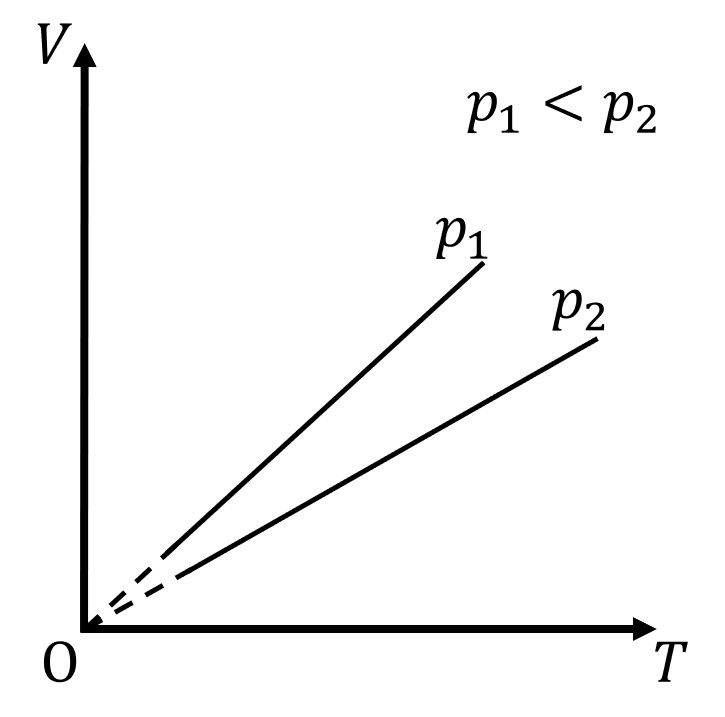
\includegraphics[scale=0.3]{../figs/VN10-PH-39-L-0291-1.jpg}
		\end{center}
	}
	\item \mkstar{2} [8]
	
	\cauhoi{
		Một xi lanh có một pit-tông có thể di chuyển dễ dàng. Ban đầu xi lanh chứa không khí có thể tích $\SI{6}{l}$ ở nhiệt độ $\SI{27}{\celsius}$. Tính thể tích của khí trong xi lanh khi đun nóng đẳng áp đến nhiệt độ $\SI{500}{K}$. Vẽ đồ thị trong hệ tọa độ $\text{O}VT$.
	}
	
	\loigiai{
		Đẳng áp (1): $V_1=\SI{6}{l}$, $T_1=\SI{300}{K}$ sang (2): $V_2=?$, $T_2=\SI{500}{K}$
		
		Vì quá trình là đẳng áp nên ta có phương trình:
		
		$$\dfrac{V_1}{T_1} = \dfrac{V_2}{T_2} \Rightarrow V_2 =\dfrac{V_1T_2}{T_1} = \SI{10}{l}.$$
		
		Đồ thị:
		\begin{center}
			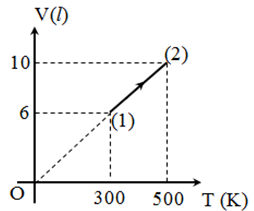
\includegraphics{../figs/VN10-2021-PH-TP032-1}
		\end{center}
	}




\end{enumerate}
\section{Lý thuyết: Phương trình trạng thái của khí lí tưởng}
\begin{enumerate}[label=\bfseries Câu \arabic*:]
	
	\item \mkstar{1} [24]
	
	\cauhoi{
		Ba thông số xác định trạng thái của một lượng khí xác định là
		\begin{mcq}(2)
			\item áp suất, thể tích và khối lượng. 
			\item áp suất, nhiệt độ và khối lượng.
			\item thể tích, trọng lượng và áp suất.
			\item áp suất, nhiệt độ và thể tích.
		\end{mcq}
	}
	
	\loigiai{
		\textbf{Đáp án: D.}
		
		Ba thông số xác định trạng thái của một lượng khí xác định là áp suất, nhiệt độ và thể tích.
	}

\item \mkstar{2} [24]

\cauhoi{
	Ở kì nén của một động cơ đốt trong 4 kì, nhiệt độ của hỗn hợp khí tăng từ $\SI{47}{\celsius}$ đến $\SI{367}{\celsius}$, còn thể tích của khí giảm từ $\SI{1.8}{l}$ xuống còn $\SI{0.3}{l}$. Áp suất của khí lúc bắt đầu nén là $\SI{1}{atm}$. Coi hỗn hợp khí như chất khí lí tưởng. Áp suất khí cuối kì nén là
	\begin{mcq}(4)
		\item $\SI{24}{atm}$. 
		\item $\SI{12}{atm}$.
		\item $\SI{6}{atm}$.
		\item $\SI{2}{atm}$.
	\end{mcq}
}

\loigiai{
	\textbf{Đáp án: B.}
	
	Biến đổi trạng thái (1): $p_1=\SI{1}{atm}$, $V_1=\SI{1.8}{l}$, $T_1=\SI{320}{K}$ sang (2): $p_2=?$, $V_2=\SI{0.3}{l}$, $T_2=\SI{640}{K}$.
	
	Áp dụng phương trình trạng thái khí lí tưởng:
	
	$$\dfrac{p_1V_1}{T_1} = \dfrac{p_2V_2}{T_2} \Rightarrow p_2 =\dfrac{p_1V_1T_2}{T_1V_2} = \SI{12}{atm}.$$
}


\item \mkstar{2} [29]

\cauhoi{
	Một cái bơm chứa $\SI{120}{cm^3}$ không khí ở nhiệt độ $\SI{25}{\celsius}$ và áp suất $\SI{e5}{Pa}$. Áp suất của không khí trong bơm khi lượng khí bị nén xuống còn $\SI{80}{cm^3}$ và nhiệt độ tăng lên tới $\SI{37}{\celsius}$ có giá trị xấp xỉ bằng bao nhiêu?
	\begin{mcq}(4)
		\item $\SI{2.5e5}{Pa}$. 
		\item $\SI{2.0e5}{Pa}$.
		\item $\SI{1.56e5}{Pa}$.
		\item $\SI{1.29e5}{Pa}$.
	\end{mcq}
}

\loigiai{
	\textbf{Đáp án: C.}
	
	Biến đổi trạng thái (1): $p_1=\SI{e5}{Pa}$, $V_1=\SI{120}{cm^3}$, $T_1=\SI{298}{K}$ sang (2): $p_2=?$, $V_2=\SI{80}{cm^3}$, $T_2=\SI{310}{K}$.
	
	Áp dụng phương trình trạng thái khí lí tưởng:
	
	$$\dfrac{p_1V_1}{T_1} = \dfrac{p_2V_2}{T_2} \Rightarrow p_2 =\dfrac{p_1V_1T_2}{T_1V_2} = \SI{1.56e5}{Pa}.$$
}
\item \mkstar{1} [16]

\cauhoi{
	Viết phương trình trạng thái khí lí tưởng, từ đó suy ra công thức tính áp suất ban đầu và thể tích lúc sau.
	
}
\loigiai{
	
	Phương trình trạng thái khí lí tưởng:
	$$\dfrac{p_1V_1}{T_1} = \dfrac{p_2V_2}{T_2}.$$
	
	Suy ra công thức tính áp suất ban đầu:
	$$p_1 = \dfrac{p_2V_2T_1}{T_2V_1}.$$
	
	Suy ra công thức tính thể tích lúc sau:
	$$V_2 = \dfrac{p_1V_1T_2}{T_1p_2}.$$
}
\item \mkstar{2} [4]

\cauhoi{
	Một bình kín có thể tích $\SI{0.4}{m^3}$, chứa khí ở $\SI{27}{\celsius}$ và áp suất $\SI{1.5}{atm}$. Khi mở nắp, áp suất khí còn $\SI{1}{atm}$, nhiệt độ còn $\SI{0}{\celsius}$. Tính thể tích khí thoát ra khỏi bình.
}
\loigiai{
	
	Biến đổi trạng thái (1): $p_1=\SI{1.5}{atm}$, $V_1=\SI{0.4}{m^3}$, $T_1=\SI{300}{K}$ sang (2): $p_2=\SI{1}{atm}$, $V_2=?$, $T_2=\SI{273}{K}$.
	
	Áp dụng phương trình trạng thái:
	
	$$\dfrac{p_1V_1}{T_1} = \dfrac{p_2V_2}{T_2} \Rightarrow V_2 =\dfrac{p_1V_1T_2}{p_2T_1} = \SI{0.546}{m^3}.$$
	
	Vậy thể tích khí thoát ra khỏi bình là $\Delta V = V_2-V_1=\SI{0.146}{m^3}$.
}
\item \mkstar{2} [10]

\cauhoi{
	Một lượng khí ở nhiệt độ $\SI{27}{\celsius}$, thể tích 5 lít và áp suất là $\SI{3}{atm}$. Làm nóng khối khí lên đến nhiệt độ $t_2$ thì thể tích lên đến 8 lít và áp suất là $\SI{2}{atm}$. Tính nhiệt độ $t_2$.
}
\loigiai{
	Biến đổi trạng thái (1): $p_1=\SI{3}{atm}$, $V_1=\SI{5}{l}$, $T_1=\SI{300}{K}$ sang (2): $p_2=\SI{2}{atm}$, $V_2=\SI{8}{l}$, $T_2=?$.
	
	Áp dụng phương trình trạng thái:
	
	$$\dfrac{p_1V_1}{T_1} = \dfrac{p_2V_2}{T_2} \Rightarrow T_2 =\dfrac{p_2V_2T_1}{p_1V_1} = \SI{320}{K}.$$
	
	Đổi $t_2=T_2-273 = \SI{47}{\celsius}$.
}
\item \mkstar{2} [11]

\cauhoi{
	Một lượng khí lí tưởng ở nhiệt độ $\SI{27}{\celsius}$, áp suất $\SI{e5}{Pa}$, thể tích 4 lít được biến đổi trạng thái qua 2 giai đoạn: nén đẳng nhiệt đến áp suất là $\SI{2e5}{Pa}$, sau đó cho dãn nở đẳng áp đến thể tích $\SI{6}{l}$. Xác định các thông số $V_2$, $p_3$.
}
\loigiai{
	
	Đẳng nhiệt (1): $p_1=\SI{e5}{Pa}$, $V_1=\SI{4}{l}$, $T_1=\SI{300}{K}$ sang (2): $p_2=\SI{2e5}{Pa}$, $V_2=?$, $T_2=T_1=\SI{300}{K}$.
	
	Áp dụng phương trình trạng thái:
	
	$$\dfrac{p_1V_1}{T_1} = \dfrac{p_2V_2}{T_2} \Rightarrow V_2 =\dfrac{p_1V_1T_2}{p_2T_1}=\dfrac{p_1V_1}{p_2} = \SI{2}{l}.$$
	
	Đẳng áp (2): $p_2=\SI{2e5}{Pa}$ sang (3): $p_3=p_2=\SI{2e5}{Pa}$.
	
	Vậy $p_3=\SI{2e5}{Pa}$.
}
\item \mkstar{2} [12]

\cauhoi{
	Một khối khí lí tưởng có nhiệt độ $\SI{27}{\celsius}$ ở trạng thái (1). Khí được biến đổi qua hai quá trình:
	\begin{itemize}
		\item Từ trạng thái (1), khí được biến đổi đẳng tích sang trạng thái (2) có áp suất $\SI{1.5}{atm}$ và nhiệt độ là $\SI{177}{\celsius}$, thể tích 10 lít.
		\item Từ trạng thái (2), khí được biến đổi đẳng áp sang trạng thái (3) có nhiệt độ $\SI{627}{\celsius}$.
	\end{itemize}
	Xác định các thông số của từng trạng thái.
}
\loigiai{
	Đẳng tích (1): $p_1=?$, $V_1=\SI{10}{l}$, $T_1=\SI{300}{K}$ sang (2): $p_2=\SI{1.5}{atm}$, $V_2=V_1=\SI{10}{l}$, $T_2=T_1=\SI{450}{K}$.
	
	Áp dụng phương trình trạng thái:
	
	$$\dfrac{p_1V_1}{T_1} = \dfrac{p_2V_2}{T_2} \Rightarrow p_1 =\dfrac{p_2V_2T_1}{V_1T_2}=\dfrac{p_2T_1}{T_2} = \SI{1}{atm}.$$
	
	Đẳng áp (2): $p_2=\SI{1.5}{atm}$, $V_2=\SI{10}{l}$, $T_2=\SI{450}{K}$ sang (3): $p_3=p_2=\SI{1.5}{atm}$, $V_3=?$, $T_3=\SI{900}{K}$.
	
	Áp dụng phương trình trạng thái:
	
	$$\dfrac{p_2V_2}{T_2} = \dfrac{p_3V_3}{T_3} \Rightarrow V_3 =\dfrac{p_2V_2T_3}{T_2p_3}=\dfrac{V_2T_3}{T_2} = \SI{20}{l}.$$
	
}
\item \mkstar{2} [15]

\cauhoi{
	Nhiệt độ ban đầu của hỗn hợp khí trong xi lanh là $T_1$, áp suất $\SI{100}{kPa}$. Nén cho thể tích khí giảm từ $\SI{1.6}{l}$ xuống đến $\SI{0.8}{l}$ thì áp suất tăng thêm $\SI{400}{kPa}$, nhiệt độ tăng thêm $\SI{450}{\celsius}$. Coi hỗn hợp khí là một chất khí thuần nhất. Tính nhiệt độ $T_1$ của khí.
	
}
\loigiai{
	
	Biến đổi trạng thái (1): $p_1=\SI{100}{kPa}$, $V_1=\SI{1.6}{l}$, $T_1$ sang (2): $p_2=p_1+\SI{400}{kPa} = \SI{500}{kPa}$, $V_2=\SI{0.8}{l}$, $T_2=T_1+\SI{450}{\celsius} = T_1 + \SI{450}{K}$.
	
	Áp dụng phương trình trạng thái khí lí tưởng:
	
	$$\dfrac{p_1V_1}{T_1} = \dfrac{p_2V_2}{T_2} \Rightarrow T_1 = \dfrac{p_1V_1T_2}{p_2V_2}=\dfrac{p_1V_2(T_1+450)}{p_2V_2} \Rightarrow T_1 = \SI{300}{K}.$$
}



\item \mkstar{2} [16]

\cauhoi{
	Một lượng khí đựng trong một xi lanh có pit-tông chuyển động được. Trạng thái của lượng khí lúc đầu là $\SI{2}{atm}$, $\SI{15}{l}$, $\SI{27}{\celsius}$. Khi pit-tông nén khí, áp suất của khí tăng lên tới $\SI{3.5}{atm}$, thể tích giảm còn $\SI{12}{l}$. Xác định nhiệt độ của khí sau khi nén.
	
}
\loigiai{
	
	Biến đổi trạng thái (1): $p_1=\SI{2}{atm}$, $V_1=\SI{15}{l}$, $T_1=\SI{300}{K}$ sang (2): $p_2=\SI{3.5}{atm}$, $V_2=\SI{12}{l}$, $T_2=?$.
	
	Áp dụng phương trình trạng thái khí lí tưởng:
	
	$$\dfrac{p_1V_1}{T_1} = \dfrac{p_2V_2}{T_2} \Rightarrow T_2 =\dfrac{p_2V_2T_1}{p_1V_1} = \SI{420}{K}.$$
	
	Đổi $t_2=T_2-273 = \SI{147}{\celsius}$.
}

\item \mkstar{2} [17]

\cauhoi{
	Một quả "bóng thám không" có thể tích 300 lít ở nhiệt độ $\SI{27}{\celsius}$ và áp suất $\SI{e5}{Pa}$ trên mặt đất. Bóng được thả ra và bay lên đến độ cao mà ở đó áp suất chỉ còn $\SI{0.5e5}{Pa}$ và nhiệt độ lúc này là $\SI{7}{\celsius}$. Tính thể tích của quả bóng ở độ cao đó.
	
}
\loigiai{
	Biến đổi trạng thái (1): $p_1=\SI{e5}{Pa}$, $V_1=\SI{300}{l}$, $T_1=\SI{300}{K}$ sang (2): $p_2=\SI{0.5e5}{Pa}$, $V_2=?$, $T_2=\SI{280}{K}$.
	
	Áp dụng phương trình trạng thái khí lí tưởng:
	
	$$\dfrac{p_1V_1}{T_1} = \dfrac{p_2V_2}{T_2} \Rightarrow V_2 =\dfrac{p_1V_1T_2}{T_1p_2} = \SI{560}{l}.$$
}
\item \mkstar{2} [18]

\cauhoi{
	Ở kì nén của một động cơ đốt trong 4 kì, nhiệt độ của hỗn hợp khí tăng từ $\SI{47}{\celsius}$ đến $\SI{367}{\celsius}$, còn thể tích của khí giảm từ $\SI{1.8}{l}$ còn $\SI{0.3}{l}$. Áp suất của khí lúc bắt đầu nén là $\SI{150}{kPa}$. Coi hỗn hợp khí như chất khí thuần nhất, áp suất cuối kì nén là bao nhiêu kPa?
	
}
\loigiai{
	
	Biến đổi trạng thái (1): $p_1=\SI{150}{kPa}$, $V_1=\SI{1.8}{l}$, $T_1=\SI{320}{K}$ sang (2): $p_2=?$, $V_2=\SI{0.3}{l}$, $T_2=\SI{640}{K}$.
	
	Áp dụng phương trình trạng thái khí lí tưởng:
	
	$$\dfrac{p_1V_1}{T_1} = \dfrac{p_2V_2}{T_2} \Rightarrow p_2 =\dfrac{p_1V_1T_2}{T_1V_2} = \SI{1800}{kPa}.$$
}
	\item \mkstar{3} [1]
	
	\cauhoi{
		\begin{enumerate}[label=\alph*)]
			\item Kể tên các đại lượng đặc trưng cho trạng thái của một lượng khí. Viết biểu thức liên hệ giữa các đại lượng này.
			\item Trong xi lanh của một động cơ đốt trong, bên dưới pit-tông có chứa hỗn hợp khí ở nhiệt độ $\SI{47}{\celsius}$. Sau đó, nén pit-tông làm cho thể tích của hỗn hợp khí giảm 10 lần thì áp suất tăng gấp 15 lần. Hãy tính nhiệt độ của hỗn hợp khí sau khi bị nén (theo đơn vị độ C). Hỗn hợp khí được xem là khí lí tưởng.
		\end{enumerate}
	}
	\loigiai{
		
		\begin{enumerate}[label=\alph*)]
			\item Các đại lượng đặc trưng cho trạng thái của một lượng khí: áp suất, thể tích, nhiệt độ (tuyệt đối). Biểu thức liên hệ: $\dfrac{pV}{T} = \text{hằng số}$ hay $\dfrac{p_1V_1}{T_1} = \dfrac{p_2V_2}{T_2}$.
			
			\item Biến đổi trạng thái (1): $p_1$, $V_1$, $T_1=\SI{320}{K}$ sang (2): $p_2=15p_1$, $V_2=\dfrac{V_1}{10}$, $T_2=?$.
			
			Áp dụng phương trình trạng thái khí lí tưởng:
			
			$$\dfrac{p_1V_1}{T_1} = \dfrac{p_2V_2}{T_2} \Rightarrow T_2 =\dfrac{p_2V_2T_1}{p_1V_1} = \SI{480}{K}.$$
			
			Đổi $t_2=T_2-273=\SI{207}{\celsius}$.
		\end{enumerate}
	}
\item \mkstar{3} [1]

\cauhoi{
	Một khối khí lí tưởng ở trạng thái ban đầu có áp suất $p_1=\SI{6}{atm}$, thể tích $V_1=\SI{2}{l}$ và nhiệt độ $t_1=\SI{27}{\celsius}$ biến đổi lần lượt qua các quá trình:
	\begin{itemize}
		\item Đẳng áp sang trạng thái 2 có nhiệt độ $t_2=\SI{627}{\celsius}$;
		\item Đẳng tích sang trạng thái 3 có áp suất $p_3=\SI{2}{atm}$;
		\item Đẳng nhiệt sang trạng thái 4 có thể tích $V_4=\SI{3}{l}$.
	\end{itemize}
	Tìm nhiệt độ ở trạng thái 3 và áp suất sau cùng của khối khí.
}
\loigiai{
	
	\begin{itemize}
		\item Đẳng áp (1): $p_1=\SI{6}{atm}$, $V_1=\SI{2}{l}$, $T_1=\SI{300}{K}$ sang (2): $p_2=p_1=\SI{6}{atm}$, $V_2=?$, $T_2=\SI{900}{K}$.
		
		Áp dụng phương trình trạng thái:
		
		$$\dfrac{p_1V_1}{T_1} = \dfrac{p_2V_2}{T_2} \Rightarrow V_2 =\dfrac{p_1V_1T_2}{p_2T_1} = \dfrac{V_1T_2}{T_1} = \SI{6}{l}.$$
		
		
		\item Đẳng tích (2): $p_2=\SI{6}{atm}$, $V_2=\SI{6}{l}$, $T_2=\SI{900}{K}$ sang (3): $p_3=\SI{2}{atm}$, $V_3=V_2=\SI{6}{l}$, $T_3=?$.
		
		Áp dụng phương trình trạng thái:
		
		$$\dfrac{p_2V_2}{T_2} = \dfrac{p_3V_3}{T_3} \Rightarrow T_3 =\dfrac{p_3V_3T_2}{p_2V_2}=\dfrac{p_3T_2}{p_2} =  \SI{300}{K}.$$
		
		
		\item Đẳng nhiệt (3): $p_3=\SI{2}{atm}$, $V_3=\SI{6}{l}$, $T_3=\SI{300}{K}$ sang (4): $p_4=?$, $V_4=\SI{3}{l}$, $T_4=T_3=\SI{300}{K}$.
		
		Áp dụng phương trình trạng thái:
		
		$$\dfrac{p_3V_3}{T_3} = \dfrac{p_4V_4}{T_4} \Rightarrow p_4 =\dfrac{p_3V_3T_4}{V_4T_3} = \dfrac{p_3V_3}{V_4} = \SI{4}{atm}.$$
		
		
	\end{itemize}
}
\item \mkstar{3} [14]

\cauhoi{
	Khi cho một lượng khí xác định được nén đẳng nhiệt từ thể tích $V_1=V_0$ sang thể tích $V_2=\dfrac{1}{3}V_0$ thì nhận thấy áp suất của lượng khí tăng thêm một lượng $\SI{2}{atm}$. Sau đó tiếp tục đun nóng đẳng tích đến khi nhiệt độ của khối khí tăng thêm $\SI{100}{\celsius}$ thì áp suất khối khí lúc này là $\SI{8}{atm}$. Xác định nhiệt độ ban đầu của lượng khí.
}
\loigiai{
	
	Đẳng nhiệt (1): $p_1$, $V_1=V_0$, $T_1=?$ sang (2): $p_2=p_1 + \SI{2}{atm}$, $V_2=\dfrac{V_0}{3}$, $T_2=T_1$.
	
	Áp dụng phương trình trạng thái:
	
	$$\dfrac{p_1V_1}{T_1} = \dfrac{p_2V_2}{T_2} \Rightarrow p_1V_1 = p_2V_2 \Rightarrow p_1 V_0 = (p_1+2) \dfrac{1}{3}V_0 \Rightarrow p_1=\SI{1}{atm}. $$
	
	Đẳng tích (2): $p_2=p_1+\SI{2}{atm}$, $V_2=\dfrac{1}{3}V_0$, $T_2=T_1$ sang (3): $p_3=\SI{8}{atm}$, $V_3=V_2=\dfrac{1}{3}V_0$, $T_3=T_2+\SI{100}{\celsius} = T_1 + \SI{100}{K}$.
	
	Áp dụng phương trình trạng thái:
	
	$$\dfrac{p_2V_2}{T_2} = \dfrac{p_3V_3}{T_3} \Rightarrow \dfrac{p_1+2}{T_1} = \dfrac{8}{T_1+100} \Rightarrow T_1 = \SI{60}{K}.$$
}
\item \mkstar{3} [20]

\cauhoi{
	Một khối khí lí tưởng có thể tích $\SI{10}{l}$, nhiệt độ $\SI{27}{\celsius}$, áp suất $\SI{2}{atm}$. Khối khí này biến đổi qua hai quá trình:
	\begin{itemize}
		\item đẳng nhiệt: áp suất tăng gấp đôi.
		\item đẳng áp: nhiệt độ sau cùng là $\SI{327}{\celsius}$.
	\end{itemize}
	Tìm các thông số trạng thái chưa biết.
}
\loigiai{
	
	Đẳng nhiệt (1): $p_1=\SI{2}{atm}$, $V_1=\SI{10}{l}$, $T_1=\SI{300}{K}$ sang (2): $p_2=2p_1 = \SI{4}{atm}$, $V_2=?$, $T_2=T_1=\SI{300}{K}$.
	
	Áp dụng phương trình trạng thái:
	
	$$\dfrac{p_1V_1}{T_1} = \dfrac{p_2V_2}{T_2} \Rightarrow V_2 = \dfrac{p_1V_1T_2}{p_2T_1} = \dfrac{p_1V_1}{p_2} =\SI{5}{l}.$$
	
	Đẳng áp (2): $p_2=\SI{4}{atm}$, $V_2=\SI{5}{l}$, $T_2=\SI{300}{K}$ sang (3): $p_3=p_2=\SI{4}{atm}$, $V_3=?$, $T_3=\SI{600}{\celsius}$.
	
	Áp dụng phương trình trạng thái:
	
	$$\dfrac{p_2V_2}{T_2} = \dfrac{p_3V_3}{T_3} \Rightarrow V_3= \dfrac{p_2V_2T_3}{T_2p_3}=\dfrac{V_2T_3}{T_2}= \SI{10}{l}.$$
}

\item \mkstar{3} [21]

\cauhoi{
	Một khối khí lí tưởng có áp suất ban đầu $p_1$, thể tích 3 lít ở nhiệt độ $\SI{27}{\celsius}$ được biến đổi trạng thái qua hai quá trình liên tiếp nhau:
	\begin{itemize}
		\item Quá trình 1: làm lạnh đẳng tích để áp suất bằng $3/4$ áp suất ban đầu;
		\item Quá trình 2: nén đẳng nhiệt đến áp suất bằng $1/2$ áp suất ban đầu.
	\end{itemize}
	\begin{enumerate}[label=\alph*)]
		\item Tính nhiệt độ khí ở trạng thái (2) theo độ C.
		\item Tính thể tích khí ở trạng thái (3).
	\end{enumerate}
	
}
\loigiai{
	\begin{enumerate}[label=\alph*)]
		\item Tính nhiệt độ khí ở trạng thái (2) theo độ C.
		Đẳng tích (1): $p_1$, $V_1=\SI{3}{l}$, $T_1=\SI{300}{K}$ sang (2): $p_2=\dfrac{3}{4}p_1$, $V_2=V_1=\SI{3}{l}$, $T_2=?$.
		
		Áp dụng phương trình trạng thái:
		
		$$\dfrac{p_1V_1}{T_1} = \dfrac{p_2V_2}{T_2} \Rightarrow T_2=\dfrac{p_2V_2T_1}{p_1V_1} = \dfrac{p_2T_1}{p_1}=\SI{225}{K}.$$
		
		Đổi $t_2 = T_2 - 273 = \SI{-48}{\celsius}$.
		
		\item Tính thể tích khí ở trạng thái (3).
		Đẳng nhiệt (2): $p_2=\dfrac{3}{4}p_1$, $V_2=\SI{3}{l}$, $T_2=\SI{225}{K}$ sang (3): $p_3=\dfrac{1}{2}p_1$, $V_3=?$, $T_3=T_2$.
		
		Áp dụng phương trình trạng thái:
		
		$$\dfrac{p_2V_2}{T_2} = \dfrac{p_3V_3}{T_3} \Rightarrow V_3 = \dfrac{p_2V_2T_3}{p_3T_2} = \dfrac{p_2V_2}{p_3} = \SI{4.5}{l}.$$
	\end{enumerate}
}

\item \mkstar{3} [22]

\cauhoi{
	Một khối khí lí tưởng có áp suất ban đầu $\SI{1.5}{atm}$, thể tích 10 lít ở nhiệt độ $\SI{87}{\celsius}$ được biến đổi trạng thái qua hai quá trình liên tiếp nhau:
	\begin{itemize}
		\item Quá trình 1: đẳng áp, nhiệt độ tuyệt đối giảm 2 lần;
		\item Quá trình 2: đẳng nhiệt, áp suất sau cùng là $\SI{1}{atm}$.
	\end{itemize}
	\begin{enumerate}[label=\alph*)]
		\item Tìm thể tích $V_2$ của khối khí sau quá trình 1.
		\item Tìm thể tích $V_3$ của khối khí sau quá trình 2.
	\end{enumerate}
	
}
\loigiai{
	\begin{enumerate}[label=\alph*)]
		\item Tìm thể tích $V_2$ của khối khí sau quá trình 1.
		Đẳng áp (1): $p_1=\SI{1.5}{atm}$, $V_1=\SI{10}{l}$, $T_1=\SI{360}{K}$ sang (2): $p_2=p_1=\SI{1.5}{atm}$, $V_2=?$, $T_2=\dfrac{T_1}{2} = \SI{180}{K}$.
		
		Áp dụng phương trình trạng thái:
		
		$$\dfrac{p_1V_1}{T_1} = \dfrac{p_2V_2}{T_2} \Rightarrow V_2=\dfrac{p_1V_1T_2}{p_2T_1} = \dfrac{V_1T_2}{T_1}=\SI{5}{l}.$$
		
		\item Tìm thể tích $V_3$ của khối khí sau quá trình 2.
		Đẳng nhiệt (2): $p_2=\SI{1.5}{atm}$, $V_2=\SI{5}{l}$, $T_2=\SI{180}{K}$ sang (3): $p_3=\SI{1}{atm}$, $V_3=?$, $T_3=T_2=\SI{180}{K}$.
		
		Áp dụng phương trình trạng thái:
		
		$$\dfrac{p_2V_2}{T_2} = \dfrac{p_3V_3}{T_3} \Rightarrow V_3 = \dfrac{p_2V_2T_3}{p_3T_2} = \dfrac{p_2V_2}{p_3} = \SI{7.5}{l}.$$
	\end{enumerate}
}

\item \mkstar{3} [23]

\cauhoi{
	Một lượng khí lí tưởng có áp suất $p_1=\SI{1}{atm}$, nhiệt độ $t_1=\SI{27}{\celsius}$ và thể tích $V_1=\SI{1}{l}$ biến đổi lần lượt qua hai quá trình sau:
	\begin{itemize}
		\item Biến đổi đẳng nhiệt tới thể tích $V_2=\SI{2}{l}$, áp suất $p_2$;
		\item Biến đổi đẳng tích tới áp suất $p_3=2p_2$, nhiệt độ $t_3$.
	\end{itemize}
	Tìm $p_2$, $t_3$.
}
\loigiai{
	Đẳng nhiệt (1): $p_1=\SI{1}{atm}$, $V_1=\SI{1}{l}$, $T_1=\SI{300}{K}$ sang (2): $p_2=?$, $V_2=\SI{2}{l}$, $T_2=T_1 = \SI{300}{K}$.
	
	Áp dụng phương trình trạng thái:
	
	$$\dfrac{p_1V_1}{T_1} = \dfrac{p_2V_2}{T_2} \Rightarrow p_2=\dfrac{p_1V_1T_2}{V_2T_1} = \dfrac{p_1V_1}{V_2}=\SI{0.5}{atm}.$$
	
	Đẳng tích (2): $p_2=\SI{0.5}{atm}$, $V_2=\SI{2}{l}$, $T_2=\SI{300}{K}$ sang (3): $p_3=2p_2=\SI{1}{atm}$, $V_3=V_2=\SI{2}{l}$, $T_3=?$.
	
	Áp dụng phương trình trạng thái:
	
	$$\dfrac{p_2V_2}{T_2} = \dfrac{p_3V_3}{T_3} \Rightarrow T_3=\dfrac{p_3V_3T_2}{p_2V_2} = \dfrac{p_3T_2}{p_2}=\SI{600}{K}.$$
	
	Đổi $t_3=T_3-273=\SI{327}{\celsius}$.
}
\item \mkstar{3} [26]

\cauhoi{
	Một khối khí lí tưởng có thể tích 5 lít, ở nhiệt độ $\SI{227}{\celsius}$ và áp suất $\SI{1}{atm}$. Cho khối khí biến đổi qua 2 quá trình liên tiếp nhau:
	\begin{itemize}
		\item Quá trình 1: làm lạnh đẳng áp cho thể tích giảm còn phân nửa thể tích ban đầu;
		\item Quá trình 2: nung nóng đẳng tích để áp suất tăng lên thêm một lượng bằng $1/2$ áp suất ban đầu.
	\end{itemize}
	Tính nhiệt độ của khối khí ở cuối mỗi quá trình ra độ C.
}
\loigiai{
	Đẳng áp (1): $p_1=\SI{1}{atm}$, $V_1=\SI{5}{l}$, $T_1=\SI{500}{K}$ sang (2): $p_2=p_1=\SI{1}{atm}$, $V_2=\dfrac{V_1}{2}=\SI{2.5}{l}$, $T_2=?$.
	
	Áp dụng phương trình trạng thái:
	
	$$\dfrac{p_1V_1}{T_1} = \dfrac{p_2V_2}{T_2} \Rightarrow T_2=\dfrac{p_2V_2T_1}{p_1V_1} = \dfrac{V_2T_1}{V_1}=\SI{250}{K}.$$
	
	Đổi $t_2=T_2-273=\SI{-23}{\celsius}$
	
	Đẳng tích (2): $p_2=\SI{1}{atm}$, $V_2=\SI{2.5}{l}$, $T_2=\SI{250}{K}$ sang (3): $p_3=1,5p_1=\SI{1.5}{atm}$, $V_3=V_2=\SI{2.5}{l}$, $T_3=?$.
	
	Áp dụng phương trình trạng thái:
	
	$$\dfrac{p_2V_2}{T_2} = \dfrac{p_3V_3}{T_3} \Rightarrow T_3=\dfrac{p_3V_3T_2}{p_2V_2} = \dfrac{p_3T_2}{p_2}=\SI{375}{K}.$$
	
	Đổi $t_3=T_3-273=\SI{102}{\celsius}$.
}
\item \mkstar{3} [29]

\cauhoi{
	Tính nhiệt độ tuyệt đối ban đầu của một khối khí xác định, biết rằng khi nhiệt độ tăng thêm $\SI{16}{\celsius}$ thì thể tích giảm đi $10\%$, còn áp suất thì tăng thêm $20\%$ so với ban đầu.
}

\loigiai{
	
	Biến đổi trạng thái (1): $p_1$, $V_1$, $T_1$ sang (2): $p_2=(1+0,2)p_1$, $V_2=(1-0,1)V_1$, $T_2=T_1+\SI{16}{\celsius}$.
	
	Áp dụng phương trình trạng thái khí lí tưởng:
	
	$$\dfrac{p_1V_1}{T_1} = \dfrac{p_2V_2}{T_2} \Rightarrow T_1 = \SI{200}{K}.$$
}
\item \mkstar{4} [3]

\cauhoi{
	
	Khối lượng riêng của không khí xác định bởi công thức $D=\dfrac{m}{V}$ (với $m$ là khối lượng không khí ứng với thể tích $V$). Ở điều kiện tiêu chuẩn ($\SI{0}{\celsius}$, $\SI{760}{mmHg}$) thì khối lượng riêng của không khí là $D_0=\SI{1.29}{kg/m^3}$. Tính khối lượng không khí chứa trong một căn phòng có thể tích $\SI{55}{m^3}$ ở vùng cao nguyên có nhiệt độ $\SI{17}{\celsius}$, áp suất $\SI{660}{mmHg}$.
}
\loigiai{
	
	Biến đổi trạng thái (1): $p_1=\SI{760}{mmHg}$, $V_1=\dfrac{m}{\SI{1.29}{kg/m^3}}$, $T_1=\SI{273}{K}$ sang (2): $p_2=\SI{660}{mmHg}$, $V_2=\SI{55}{m^3}$, $T_2=\SI{290}{K}$.
	
	Áp dụng phương trình trạng thái:
	
	$$\dfrac{p_1V_1}{T_1} = \dfrac{p_2V_2}{T_2} \Rightarrow m = \SI{58}{kg}.$$
}


	



\item \mkstar{4} [17]

\cauhoi{
	Tính khối lượng riêng của không khí ở đỉnh núi cao $\SI{3220}{m}$. Biết rằng mỗi khi lên cao $\SI{10}{m}$ thì áp suất khí quyển giảm $\SI{1}{mmHg}$ và nhiệt độ trên đỉnh núi là $\SI{2}{\celsius}$. Khối lượng riêng của không khí ở điều kiện chuẩn (áp suất $\SI{760}{mmHg}$ và nhiệt độ $\SI{0}{\celsius}$) là $\SI{1.29}{kg/m^3}$.
}
\loigiai{
	
	Áp suất trên đỉnh núi:
	$$p_2 = p_1 - \dfrac{\SI{3220}{m}}{\SI{10}{m}} \cdot \SI{1}{mmHg} = p_1 - \SI{322}{mmHg} = \SI{760}{mmHg} - \SI{322}{mmHg} = \SI{438}{mmHg}.$$
	
	Vì $m_1 = m_2$ nên $V_1D_1 = V_2D_2$, áp dụng phương trình trạng thái:
	$$\dfrac{p_1V_1}{T_1} = \dfrac{p_2V_2}{T_2} \Rightarrow \dfrac{p_1}{D_1 T_1} = \dfrac{p_2}{D_2 T_2} \Rightarrow D_2 = \SI{0.74}{kg/m^3}.$$
}





\item \mkstar{4} [23]

\cauhoi{
	Có hai bình cầu nối với nhau bằng một ống dẫn có khóa. Bình thứ nhất có dung tích $V_1=\SI{15}{l}$ chứa khí có áp suất $p_1=\SI{2e5}{Pa}$. Bình thứ hai có dung tích $V_2=\SI{5}{l}$. Mở khóa nhẹ nhàng để hai bình thông nhau sao cho nhiệt độ của hai bình luôn bằng nhiệt độ phòng. Biết thể tích của ống dẫn là nhỏ và có thể bỏ qua. Tính áp suất trong hai bình khi đã cân bằng. Xét hai trường hợp sau:
	\begin{enumerate}[label=\alph*)]
		\item Ban đầu bình 2 không chứa khí.
		\item Ban đầu bình 2 chứa khí cùng loại với bình 1, áp suất là $p_2=\SI{1.2e5}{Pa}$.
	\end{enumerate}
	
}
\loigiai{
	Nhiệt độ của hai bình luôn bằng nhiệt độ phòng nên quá trình là đẳng nhiệt.
	\begin{enumerate}[label=\alph*)]
		\item Ban đầu bình 2 không chứa khí.
		
		Khi mở khóa, 15 lít khí trong bình 1 sẽ tràn vào bình 2, làm cho thể tích của toàn bộ lượng khí của hệ tăng từ 15 lít lên đến $V'=\SI{20}{l}$.
		
		Khi cân bằng, áp suất khí trong bình 1 bằng áp suất khí trong bình 2, do đó $p'=p_1' = p_2'$. Áp dụng định luật Bôi-lơ - Ma-ri-ốt cho lượng khí trong toàn bộ hệ:
		$$p_1V_1 = p' V'\Rightarrow p' = \SI{1.5e5}{Pa}.$$
		
		\item Ban đầu bình 2 chứa khí cùng loại với bình 1, áp suất là $p_2=\SI{1.2e5}{Pa}$.
		
		Ta thực hiện phương pháp cô lập từng phần bình, nghĩa là xem như lúc đầu chỉ có bình 1 chứa khí, hoặc chỉ có bình 2 chứa khí. Sau đó cộng áp suất riêng phần của hai bình thì được áp suất khí sau khi cân bằng.
		
		Áp dụng định luật Bôi-lơ - Ma-ri-ốt cho lượng khí trong bình 2, tính được áp suất riêng phần do khí trong bình 2 gây ra lúc sau:
		$$p_2V_2 = p_2'' V_2'' \Rightarrow p_2'' = \dfrac{p_2V_2}{V_2''} = \dfrac{p_2V_2}{V'} = \SI{0.3e5}{Pa}.$$
		
		
		Áp dụng định luật Bôi-lơ - Ma-ri-ốt cho lượng khí trong bình 1, tính được áp suất riêng phần do khí trong bình 1 gây ra lúc sau:
		$$p_1V_1 = p_1'' V_1'' \Rightarrow p_1'' = \dfrac{p_1V_1}{V_1''} = \dfrac{p_1V_1}{V'} = \SI{1.5e5}{Pa}.$$
		
		Áp suất khi cân bằng: $p''=p_1'' + p_2'' = \SI{1.8e5}{Pa}$.
	\end{enumerate}
}

\end{enumerate}

\section{Lý thuyết: Đồ thị biến đổi trạng thái khí lí tưởng}
\begin{enumerate}[label=\bfseries Câu \arabic*:]
	
	\item \mkstar{2} [4]
	
	\cauhoi{
		
			Một lượng khí lí tưởng xác định biến đổi theo chu trình như hình vẽ bên. Nếu chuyển đồ thị sang hệ trục tọa độ $(p,V)$ thì đáp án nào mô tả tương đương?
		
		
		\begin{center}
			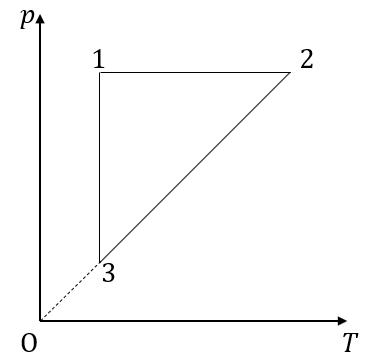
\includegraphics[scale=0.7]{../figs/VN10-2021-PH-TP032-2}
		\end{center}
		\begin{mcq}(2)
			\item 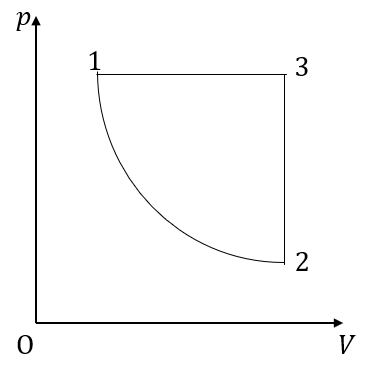
\includegraphics[scale=0.7]{../figs/VN10-2021-PH-TP032-3} 
			\item 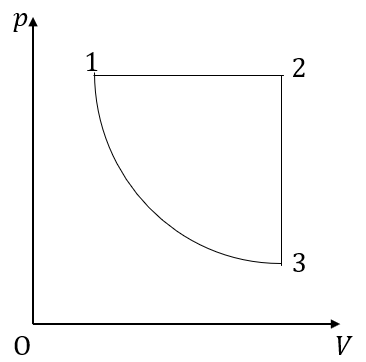
\includegraphics[scale=0.7]{../figs/VN10-2021-PH-TP032-4}
			\item 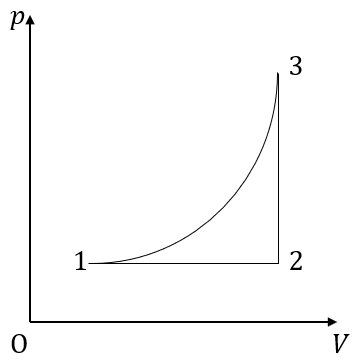
\includegraphics[scale=0.7]{../figs/VN10-2021-PH-TP032-5}
			\item 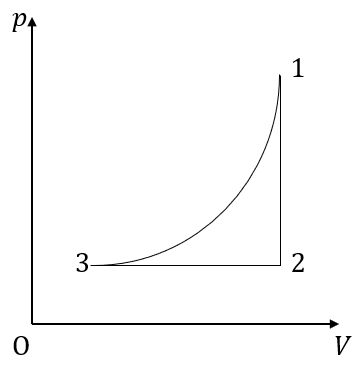
\includegraphics[scale=0.7]{../figs/VN10-2021-PH-TP032-6}
		\end{mcq}
	}
	
	\loigiai{
		\textbf{Đáp án: B.}
		
		Từ (1) sang (2) là quá trình đẳng áp, nhiệt độ tăng;
		
		Từ (2) sang (3) là quá trình đẳng tích, áp suất giảm;
		
		Từ (3) sang (1) là quá trình đẳng nhiệt, áp suất tăng.
	}
\item \mkstar{1} [10]

\cauhoi{
	Các đồ thị sau đây biểu diễn quá trình nào?
	\begin{center}
		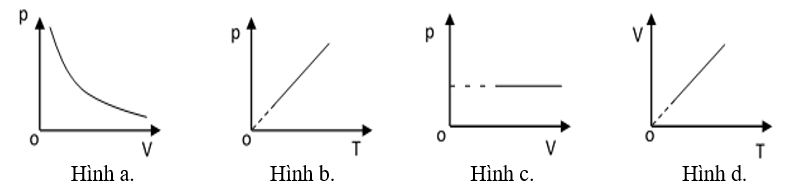
\includegraphics{../figs/VN10-2021-PH-TP032-12}
	\end{center}
}
\loigiai{
	\begin{itemize}
		\item Hình a: đẳng nhiệt;
		\item Hình b: đẳng tích;
		\item Hình c: đẳng áp;
		\item Hình d: đẳng áp.
	\end{itemize}
}
\item \mkstar{1} [13]

\cauhoi{
	Cho đồ thị như hình vẽ. Hãy đọc tên các quá trình biến đổi trạng thái.
	\begin{center}
		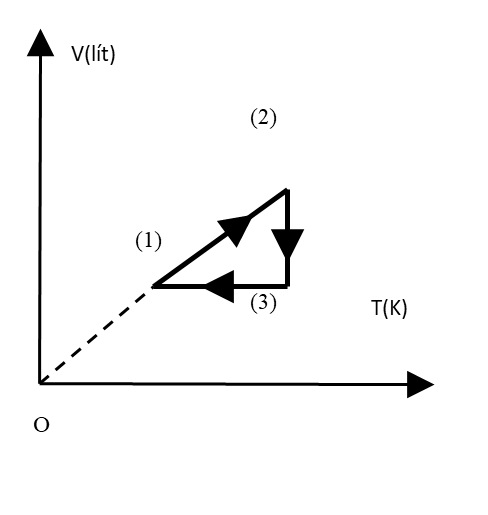
\includegraphics[scale=2]{../figs/VN10-2021-PH-TP032-15}
	\end{center}
	
}
\loigiai{
	Từ (1) sang (2): quá trình đẳng áp;
	
	Từ (2) sang (3): quá trình đẳng nhiệt;
	
	Từ (3) sang (1): quá trình đẳng tích.
}


	\item \mkstar{2} [2]

\cauhoi{
	Hình bên thể hiện quá trình chuyển từ trạng thái (1) sang (2) của một khối khí thì khí bị nén hay giãn? Giải thích.
	\begin{center}
		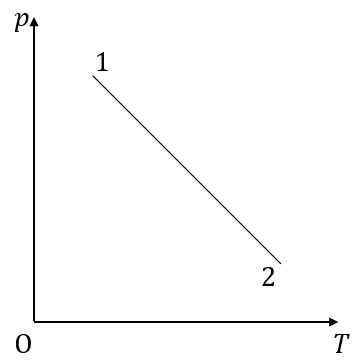
\includegraphics[scale=0.7]{../figs/VN10-2021-PH-TP032-8}
	\end{center}
}

\loigiai{
	
	Trong quá trình từ (1) sang (2) áp suất giảm, nhiệt độ tăng. Ta có $\dfrac{pV}{T} = \text{hằng số} \Rightarrow V \sim \dfrac{T}{p}$. Khi $T$ tăng, $p$ giảm thì $V$ tăng. Khối khí bị giãn.
}

	\item \mkstar{2} [3]

\cauhoi{
	Một khối khí lí tưởng được biến đổi trạng thái theo một chu trình kín như hình vẽ. Cho biết áp suất ban đầu của khối khí $p_1=\SI{9}{atm}$. Tính nhiệt độ $T_1$ và áp suất $p_3$ của khối khí.
	\begin{center}
		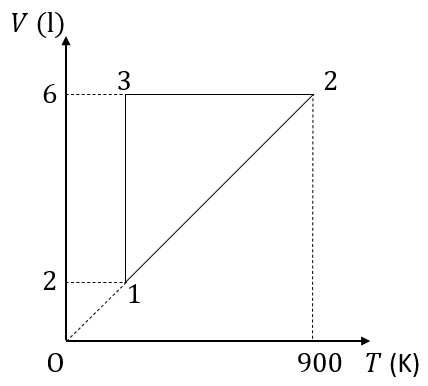
\includegraphics[scale=0.7]{../figs/VN10-2021-PH-TP032-9}
	\end{center}
}

\loigiai{
	Đẳng áp (1): $V_1=\SI{2}{l}$, $T_1=?$ sang (2): $V_2=\SI{6}{l}$, $T_2=\SI{900}{K}$.
	
	Vì quá trình là đẳng áp nên ta có phương trình:
	
	$$\dfrac{V_1}{T_1} = \dfrac{V_2}{T_2} \Rightarrow T_1 =\dfrac{V_1T_2}{V_2} = \SI{300}{K}.$$
	
	Đẳng tích (2): $p_2$, $T_2=\SI{900}{K}$ sang (3): $p_3=?$, $T_3=\SI{300}{K}$.
	
	Vì quá trình là đẳng tích nên ta có phương trình:
	
	$$\dfrac{p_2}{T_2} = \dfrac{p_3}{T_3} \Rightarrow p_2 =\dfrac{p_3T_2}{T_3} = 3p_3.$$
	
	Mà $p_1=p_2=\SI{9}{atm}$ nên $p_3 = \dfrac{p_2}{3} = \SI{3}{atm}$.
	
}

	\item \mkstar{2} [5]

\cauhoi{
	
		Một khối khí thực hiện một chu trình như hình vẽ. Cho $p_1=\SI{5e5}{Pa}$, $V_1=\SI{2.5}{l}$, $T_2=\SI{300}{K}$, $V_2=\SI{6.25}{l}$.
		\begin{enumerate}[label=\alph*)]
			\item Nêu tên gọi các đẳng quá trình trong chu trình.
			\item Tính $p_2$ và $T_3$.
		\end{enumerate}


	\begin{center}
		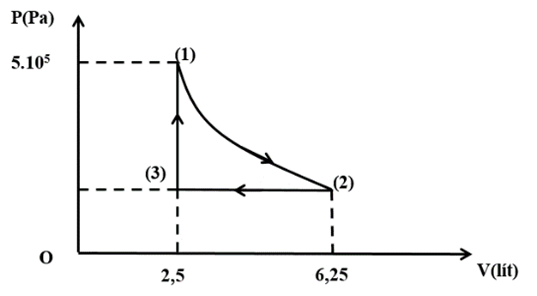
\includegraphics[scale=1.2]{../figs/VN10-2021-PH-TP032-10}
	\end{center}
	
}

\loigiai{
	\begin{enumerate}[label=\alph*)]
		\item Nêu tên gọi các đẳng quá trình trong chu trình.
		
		Từ (1) sang (2): đẳng nhiệt;
		
		Từ (2) sang (3): đẳng áp;
		
		Từ (3) sang (1): đẳng tích.
		
		\item Tính $p_2$ và $T_3$.
		
		Đẳng nhiệt (1): $V_1=\SI{2.5}{l}$, $p_1=\SI{5e5}{Pa}$ sang (2): $p_2=?$, $V_2=\SI{6.25}{l}$.
		
		Vì quá trình là đẳng nhiệt nên ta có phương trình:
		
		$$p_1V_1 = p_2V_2 \Rightarrow p_2 =\dfrac{p_1V_1}{V_2} = \SI{2e5}{Pa}.$$
		
		Đẳng áp (2): $V_2=\SI{6.25}{l}$, $T_2=\SI{300}{K}$ sang (3): $V_3=\SI{2.5}{l}$, $T_3=?$.
		
		Vì quá trình là đẳng áp nên ta có phương trình:
		
		$$\dfrac{V_2}{T_2} = \dfrac{V_3}{T_3} \Rightarrow T_3 =\dfrac{V_3T_2}{V_2} = \SI{120}{K}.$$
		
	\end{enumerate}
}
	
	\item \mkstar{2} [8]
	
	\cauhoi{
		Một khối khí lí tưởng thực hiện các quá trình biến đổi trạng thái theo đồ thị bên.
		\begin{enumerate}[label=\alph*)]
			\item Nêu tên các quá trình biến đổi trạng thái trên đồ thị.
			\item Biết rằng trạng thái 1 có các thông số $V_1=\SI{10}{l}$, $p_1=\SI{2}{atm}$, $T_1=\SI{200}{K}$, trạng thái 2 có áp suất $p_2=\SI{8}{atm}$. Tính thể tích ở trạng thái 2 và nhiệt độ tuyệt đối ở trạng thái 3.
		\end{enumerate}
	\begin{center}
		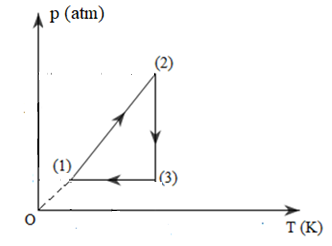
\includegraphics[scale=1.2]{../figs/VN10-2021-PH-TP032-11}
	\end{center}
		
	}
	\loigiai{
		
		\begin{enumerate}[label=\alph*)]
			\item Nêu tên các quá trình biến đổi trạng thái trên đồ thị.
			
			Từ (1) sang (2): đẳng tích;
			
			Từ (2) sang (3): đẳng nhiệt;
			
			Từ (3) sang (1): đẳng áp.
			
			\item Biết rằng trạng thái 1 có các thông số $V_1=\SI{10}{l}$, $p_1=\SI{2}{atm}$, $T_1=\SI{200}{K}$, trạng thái 2 có áp suất $p_2=\SI{8}{atm}$. Tính thể tích ở trạng thái 2 và nhiệt độ tuyệt đối ở trạng thái 3.
			
			Từ (1) sang (2) là đẳng tích nên $V_2=V_1 = \SI{10}{l}$.
			
			Đẳng tích (1): $p_1=\SI{2}{atm}$, $T_1=\SI{200}{K}$ sang (2): $p_2=\SI{8}{atm}$, $T_2=?$.
			
			Vì quá trình là đẳng tích nên ta có phương trình:
			
			$$\dfrac{p_1}{T_1} = \dfrac{p_2}{T_2} \Rightarrow T_2 =\dfrac{p_2T_1}{p_1} = \SI{800}{K}.$$
			
			Từ (2) sang (3) là đẳng nhiệt nên $T_3=T_2=\SI{800}{K}$.
			
		\end{enumerate}
	}



\item \mkstar{2} [10]

\cauhoi{
	Giải thích các quá trình biến đổi trạng thái của một khối khí trong đồ thị $(p,T)$ ở hình bên. Hãy biểu diễn lại các quá trình trong hệ tọa độ $(V,T)$.
	\begin{center}
		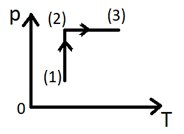
\includegraphics[scale=0.8]{../figs/VN10-2021-PH-TP032-13}
	\end{center}
	
}
\loigiai{
	Từ (1) sang (2) là quá trình đẳng nhiệt, áp suất tăng;
	
	Từ (2) sang (3) là quá trình đẳng áp, nhiệt độ tăng.
	
	Biểu diễn lại các quá trình trong hệ tọa độ $(V,T)$:
	\begin{center}
	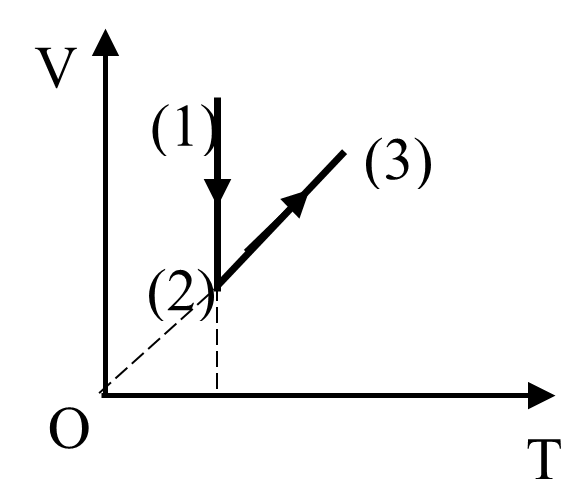
\includegraphics[scale=0.9]{../figs/VN10-2021-PH-TP032-14}
	\end{center}	
	
}



\item \mkstar{2} [14]

\cauhoi{
	Một khối khí lí tưởng biến đổi trạng thái qua hai quá trình liên tiếp được biểu diễn bằng đồ thị sau. Gọi tên các đẳng quá trình. Dựa vào các định luật hãy so sánh nhiệt độ ở trạng thái 1 với nhiệt độ ở trạng thái 3.
	\begin{center}
		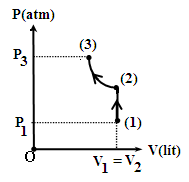
\includegraphics{../figs/VN10-2021-PH-TP032-16}
	\end{center}
	
}
\loigiai{
	
	Từ (1) sang (2): quá trình đẳng tích;
	
	Từ (2) sang (3): quá trình đẳng nhiệt.
	
	Từ (1) sang (2) áp suất tăng nên nhiệt độ tăng (áp suất tỉ lệ thuận với nhiệt độ). Vậy $T_2 > T_1$ suy ra $T_3>T_1$ (vì đẳng nhiệt $T_3=T_2$).
}
	\item \mkstar{2} [16]

\cauhoi{
	Một lượng khí đựng trong một xi lanh có pit-tông chuyển động được. Trạng thái của lượng khí lúc đầu là $\SI{2}{atm}$, $\SI{15}{l}$, $\SI{27}{\celsius}$. Khi pit-tông nén khí, áp suất của khí tăng lên tới $\SI{3.5}{atm}$, thể tích giảm còn $\SI{12}{l}$. Giả sử trong quá trình nén khí ở trên mà nhiệt độ khí không đổi, hãy vẽ đường đẳng nhiệt trong hệ trục $p\text{O}V$.
	
}
\loigiai{
	Vẽ đường đẳng nhiệt trong hệ trục $p\text{O}V$:
	\begin{center}
		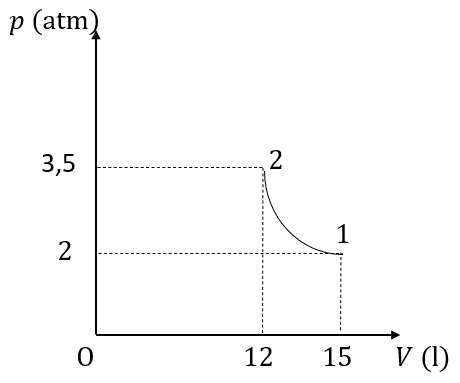
\includegraphics[scale=0.7]{../figs/VN10-2021-PH-TP032-18}
	\end{center}
}
\item \mkstar{2} [32]

\cauhoi{
	Một lượng khí lí tưởng biến đổi trạng thái như hình dưới.
	\begin{enumerate}[label=\alph*)]
		\item Gọi tên các quá trình biến đổi trạng thái của lượng khí trên.
		\item Tính thể tích ở trạng thái (1), biết thể tích ở trạng thái (2) là 10 lít.
	\end{enumerate}
	
	\begin{center}
		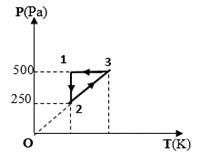
\includegraphics{../figs/VN10-2021-PH-TP032-22}
	\end{center}
}
\loigiai{
	
	\begin{enumerate}[label=\alph*)]
		\item Gọi tên các quá trình biến đổi trạng thái của lượng khí trên.
		
		Từ (1) sang (2): quá trình đẳng nhiệt;
		
		Từ (2) sang (3): quá trình đẳng tích;
		
		Từ (3) sang (1): quá trình đẳng áp.
		
		\item Tính thể tích ở trạng thái (1), biết thể tích ở trạng thái (2) là 10 lít.
		
		Đẳng nhiệt (1): $p_1=\SI{500}{Pa}$, $V_1=?$ sang (2): $p_2=\SI{250}{K}$, $V_2=\SI{10}{l}$
		
		Vì quá trình là đẳng nhiệt nên ta có phương trình:
		
		$$p_1V_1 = p_2V_2 \Rightarrow V_1 =\dfrac{p_2V_2}{p_1} = \SI{5}{l}.$$
	\end{enumerate}
}
		\item \mkstar{3} [1]
	
	\cauhoi{
		Một khối khí lí tưởng ở trạng thái ban đầu có áp suất $p_1=\SI{6}{atm}$, thể tích $V_1=\SI{2}{l}$ và nhiệt độ $t_1=\SI{27}{\celsius}$ biến đổi lần lượt qua các quá trình:
		\begin{itemize}
			\item Đẳng áp sang trạng thái 2 có nhiệt độ $t_2=\SI{627}{\celsius}$;
			\item Đẳng tích sang trạng thái 3 có áp suất $p_3=\SI{2}{atm}$;
			\item Đẳng nhiệt sang trạng thái 4 có thể tích $V_4=\SI{3}{l}$.
		\end{itemize}
		Vẽ đường biểu diễn các biến đổi trên trong hệ tọa độ $(\text{O}pV)$.
	}
	\loigiai{
		
		\begin{itemize}
			\item Đẳng áp (1): $p_1=\SI{6}{atm}$, $V_1=\SI{2}{l}$, $T_1=\SI{300}{K}$ sang (2): $p_2=p_1=\SI{6}{atm}$, $V_2=?$, $T_2=\SI{900}{K}$.
			
			Áp dụng phương trình trạng thái:
			
			$$\dfrac{p_1V_1}{T_1} = \dfrac{p_2V_2}{T_2} \Rightarrow V_2 =\dfrac{p_1V_1T_2}{p_2T_1} = \dfrac{V_1T_2}{T_1} = \SI{6}{l}.$$
			
			
			\item Đẳng tích (2): $p_2=\SI{6}{atm}$, $V_2=\SI{6}{l}$, $T_2=\SI{900}{K}$ sang (3): $p_3=\SI{2}{atm}$, $V_3=V_2=\SI{6}{l}$, $T_3=?$.
			
			Áp dụng phương trình trạng thái:
			
			$$\dfrac{p_2V_2}{T_2} = \dfrac{p_3V_3}{T_3} \Rightarrow T_3 =\dfrac{p_3V_3T_2}{p_2V_2}=\dfrac{p_3T_2}{p_2} =  \SI{300}{K}.$$
			
			
			\item Đẳng nhiệt (3): $p_3=\SI{2}{atm}$, $V_3=\SI{6}{l}$, $T_3=\SI{300}{K}$ sang (4): $p_4=?$, $V_4=\SI{3}{l}$, $T_4=T_3=\SI{300}{K}$.
			
			Áp dụng phương trình trạng thái:
			
			$$\dfrac{p_3V_3}{T_3} = \dfrac{p_4V_4}{T_4} \Rightarrow p_4 =\dfrac{p_3V_3T_4}{V_4T_3} = \dfrac{p_3V_3}{V_4} = \SI{4}{atm}.$$
			
			
		\end{itemize}
		Vẽ đường biểu diễn các biến đổi trên trong hệ tọa độ $(\text{O}pV)$:
		\begin{center}
			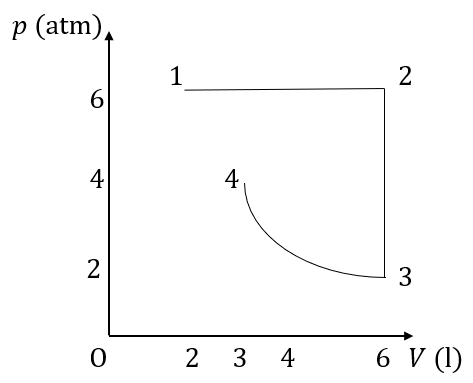
\includegraphics[scale=0.7]{../figs/VN10-2021-PH-TP032-7}
		\end{center}
	}
	\item \mkstar{3} [14]
	
	\cauhoi{
		Khi cho một lượng khí xác định được nén đẳng nhiệt từ thể tích $V_1=V_0$ sang thể tích $V_2=\dfrac{1}{3}V_0$ thì nhân thấy áp suất của lượng khí tăng thêm một lượng $\SI{2}{atm}$. Sau đó tiếp tục đun nóng đẳng tích đến khi nhiệt độ của khối khí tăng thêm $\SI{100}{\celsius}$ thì áp suất khối khí lúc này là $\SI{8}{atm}$. Vẽ đồ thị biểu diễn quá trình biến đổi các trạng thái trên trong hệ tọa độ $(\text{O}p,\text{O}T)$ với $\text{O}T$ là trục hoành.
	}
	\loigiai{
		
		Đẳng nhiệt (1): $p_1$, $V_1=V_0$, $T_1=?$ sang (2): $p_2=p_1 + \SI{2}{atm}$, $V_2=\dfrac{V_0}{3}$, $T_2=T_1$.
		
		Áp dụng phương trình trạng thái:
		
		$$\dfrac{p_1V_1}{T_1} = \dfrac{p_2V_2}{T_2} \Rightarrow p_1V_1 = p_2V_2 \Rightarrow p_1 V_0 = (p_1+2) \dfrac{1}{3}V_0 \Rightarrow p_1=\SI{1}{atm}.$$
		
		Đẳng tích (2): $p_2=p_1+\SI{2}{atm}=\SI{3}{atm}$, $V_2=\dfrac{1}{3}V_0$, $T_2=T_1$ sang (3): $p_3=\SI{8}{atm}$, $V_3=V_2=\dfrac{1}{3}V_0$, $T_3=T_2+\SI{100}{\celsius} = T_1 + \SI{100}{K}$.
		
		Áp dụng phương trình trạng thái:
		
		$$\dfrac{p_2V_2}{T_2} = \dfrac{p_3V_3}{T_3} \Rightarrow \dfrac{3}{T_1} = \dfrac{8}{T_1+100} \Rightarrow T_1 = \SI{60}{K}.$$
		
		Vẽ đồ thị biểu diễn quá trình biến đổi các trạng thái trên trong hệ tọa độ $(\text{O}p,\text{O}T)$ với $\text{O}T$ là trục hoành:
		\begin{center}
			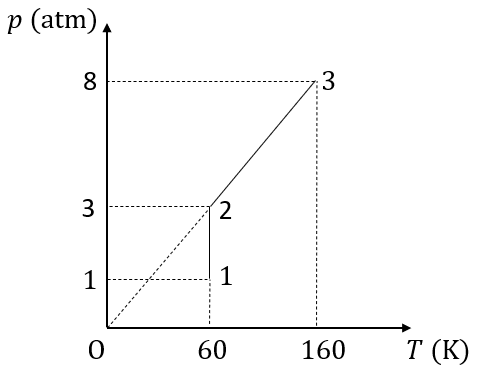
\includegraphics[scale=0.7]{../figs/VN10-2021-PH-TP032-17}
		\end{center}
	}

	\item \mkstar{3} [21]
	
	\cauhoi{
		Một khối khí lí tưởng có áp suất ban đầu $p_1$, thể tích 3 lít ở nhiệt độ $\SI{27}{\celsius}$ được biến đổi trạng thái qua hai quá trình liên tiếp nhau:
		\begin{itemize}
			\item Quá trình 1: làm lạnh đẳng tích để áp suất bằng $3/4$ áp suất ban đầu;
			\item Quá trình 2: nén đẳng nhiệt đến áp suất bằng $1/2$ áp suất ban đầu.
		\end{itemize}
	Biểu diễn các quá trình biến đổi trong hệ tọa độ $(p,V)$.
		
	}
	\loigiai{
		\begin{enumerate}[label=\alph*)]
			\item Tính nhiệt độ khí ở trạng thái (2) theo độ C.
			Đẳng tích (1): $p_1$, $V_1=\SI{3}{l}$, $T_1=\SI{300}{K}$ sang (2): $p_2=\dfrac{3}{4}p_1$, $V_2=V_1=\SI{3}{l}$, $T_2=?$.
			
			Áp dụng phương trình trạng thái:
			
			$$\dfrac{p_1V_1}{T_1} = \dfrac{p_2V_2}{T_2} \Rightarrow T_2=\dfrac{p_2V_2T_1}{p_1V_1} = \dfrac{p_2T_1}{p_1}=\SI{225}{K}.$$
			
			
			\item Tính thể tích khí ở trạng thái (3).
			Đẳng nhiệt (2): $p_2=\dfrac{3}{4}p_1$, $V_2=\SI{3}{l}$, $T_2=\SI{225}{K}$ sang (3): $p_3=\dfrac{1}{2}p_1$, $V_3=?$, $T_3=T_2$.
			
			Áp dụng phương trình trạng thái:
			
			$$\dfrac{p_2V_2}{T_2} = \dfrac{p_3V_3}{T_3} \Rightarrow V_3 = \dfrac{p_2V_2T_3}{p_3T_2} = \dfrac{p_2V_2}{p_3} = \SI{4.5}{l}.$$
		\end{enumerate}
	
	Biểu diễn các quá trình biến đổi trong hệ tọa độ $(p,V)$.
	\begin{center}
		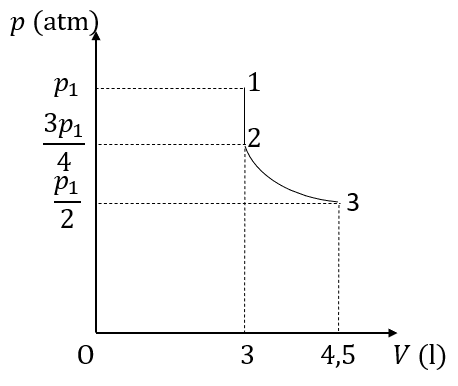
\includegraphics[scale=0.7]{../figs/VN10-2021-PH-TP032-19}
	\end{center}
	
	}

\item \mkstar{3} [23]

\cauhoi{
	Một lượng khí lí tưởng có áp suất $p_1=\SI{1}{atm}$, nhiệt độ $t_1=\SI{27}{\celsius}$ và thể tích $V_1=\SI{1}{l}$ biến đổi lần lượt qua hai quá trình sau:
	\begin{itemize}
		\item Biến đổi đẳng nhiệt tới thể tích $V_2=\SI{2}{l}$, áp suất $p_2$;
		\item Biến đổi đẳng tích tới áp suất $p_3=2p_2$, nhiệt độ $t_3$.
	\end{itemize}
	Vẽ đồ thị biểu diễn hai quá trình biến đổi trạng thái trên của khối khí trong hệ trục $(p,V)$.
}
\loigiai{
	Đẳng nhiệt (1): $p_1=\SI{1}{atm}$, $V_1=\SI{1}{l}$, $T_1=\SI{300}{K}$ sang (2): $p_2=?$, $V_2=\SI{2}{l}$, $T_2=T_1 = \SI{300}{K}$.
	
	Áp dụng phương trình trạng thái:
	
	$$\dfrac{p_1V_1}{T_1} = \dfrac{p_2V_2}{T_2} \Rightarrow p_2=\dfrac{p_1V_1T_2}{V_2T_1} = \dfrac{p_1V_1}{V_2}=\SI{0.5}{atm}.$$
	
	Đẳng tích (2): $p_2=\SI{0.5}{atm}$, $V_2=\SI{2}{l}$, $T_2=\SI{300}{K}$ sang (3): $p_3=2p_2=\SI{1}{atm}$, $V_3=V_2=\SI{2}{l}$, $T_3=?$.
	
	Áp dụng phương trình trạng thái:
	
	$$\dfrac{p_2V_2}{T_2} = \dfrac{p_3V_3}{T_3} \Rightarrow T_3=\dfrac{p_3V_3T_2}{p_2V_2} = \dfrac{p_3T_2}{p_2}=\SI{600}{K}.$$
	
	Vẽ đồ thị biểu diễn hai quá trình biến đổi trạng thái trên của khối khí trong hệ trục $(p,V)$:
	
	\begin{center}
		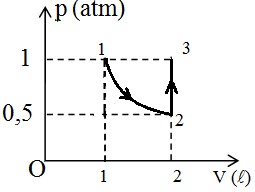
\includegraphics[scale=0.8]{../figs/VN10-2021-PH-TP032-20}
	\end{center}
}

\item \mkstar{3} [12]

\cauhoi{
	Một khối khí lí tưởng có nhiệt độ $\SI{27}{\celsius}$ ở trạng thái (1). Khí được biến đổi qua hai quá trình:
	\begin{itemize}
		\item Từ trạng thái (1), khí được biến đổi đẳng tích sang trạng thái (2) có áp suất $\SI{1.5}{atm}$ và nhiệt độ là $\SI{177}{\celsius}$, thể tích 10 lít.
		\item Từ trạng thái (2), khí được biến đổi đẳng áp sang trạng thái (3) có nhiệt độ $\SI{627}{\celsius}$.
	\end{itemize}
	Vẽ đồ thị biểu diễn quá trình biến đổi trạng thái trên trong hệ tọa độ $\text{O}p, \text{O}T$ với $\text{O}T$ là trục hoành, $\text{O}p$ là trục tung.
}
\loigiai{
	Đẳng tích (1): $p_1=?$, $V_1=\SI{10}{l}$, $T_1=\SI{300}{K}$ sang (2): $p_2=\SI{1.5}{atm}$, $V_2=V_1=\SI{10}{l}$, $T_2=T_1=\SI{450}{K}$.
	
	Áp dụng phương trình trạng thái:
	
	$$\dfrac{p_1V_1}{T_1} = \dfrac{p_2V_2}{T_2} \Rightarrow p_1 =\dfrac{p_2V_2T_1}{V_1T_2}=\dfrac{p_2T_1}{T_2} = \SI{1}{atm}.$$
	
	Đẳng áp (2): $p_2=\SI{1.5}{atm}$, $V_2=\SI{10}{l}$, $T_2=\SI{450}{K}$ sang (3): $p_3=p_2=\SI{1.5}{atm}$, $V_3=?$, $T_3=\SI{900}{K}$.
	
	Áp dụng phương trình trạng thái:
	
	$$\dfrac{p_2V_2}{T_2} = \dfrac{p_3V_3}{T_3} \Rightarrow V_3 =\dfrac{p_2V_2T_3}{T_2p_3}=\dfrac{V_2T_3}{T_2} = \SI{20}{l}.$$
	
	Vẽ đồ thị biểu diễn quá trình biến đổi trạng thái trên trong hệ tọa độ $\text{O}p, \text{O}T$ với $\text{O}T$ là trục hoành, $\text{O}p$ là trục tung.
	
	\begin{center}
		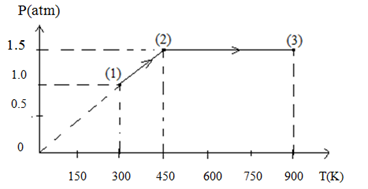
\includegraphics{../figs/VN10-2021-PH-TP032-21}
	\end{center}
	
}
\item \mkstar{3} [11]

\cauhoi{
	Một lượng khí lí tưởng ở nhiệt độ $\SI{27}{\celsius}$, áp suất $\SI{e5}{Pa}$, thể tích 4 lít được biến đổi trạng thái qua 2 giai đoạn: nén đẳng nhiệt đến áp suất là $\SI{2e5}{Pa}$, sau đó cho dãn nở đẳng áp đến thể tích $\SI{6}{l}$. Vẽ đồ thị mô tả quá trình biến đổi của khối khí trên trong hệ tọa độ $(p,T)$.
}
\loigiai{
	
	Đẳng nhiệt (1): $p_1=\SI{e5}{Pa}$, $V_1=\SI{4}{l}$, $T_1=\SI{300}{K}$ sang (2): $p_2=\SI{2e5}{Pa}$, $V_2=?$, $T_2=T_1=\SI{300}{K}$.
	
	Áp dụng phương trình trạng thái:
	
	$$\dfrac{p_1V_1}{T_1} = \dfrac{p_2V_2}{T_2} \Rightarrow V_2 =\dfrac{p_1V_1T_2}{p_2T_1}=\dfrac{p_1V_1}{p_2} = \SI{2}{l}.$$
	
	Đẳng áp (2): $p_2=\SI{2e5}{Pa}$ sang (3): $p_3=p_2=\SI{2e5}{Pa}$.
	
	Vẽ đồ thị mô tả quá trình biến đổi của khối khí trên trong hệ tọa độ $(p,T)$:
	\begin{center}
		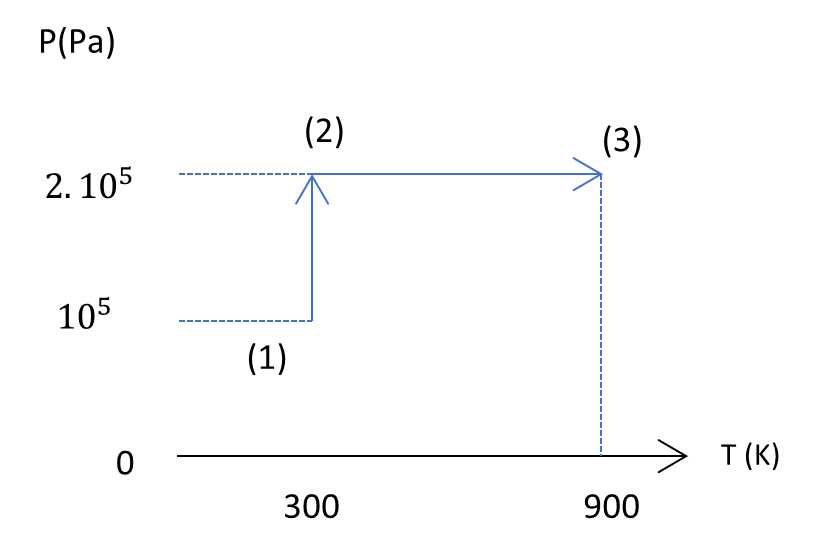
\includegraphics[scale=1.3]{../figs/VN10-2021-PH-TP032-23}
	\end{center}
}
\end{enumerate}	
\whiteBGstarEnd
	\stopcontents[mychapters]
	
\chapter[\textbf{Ôn tập: Chương V. Chất khí}]{Ôn tập: Chương V. Chất khí}
	\startcontents[chapters]
	\printcontents[chapters]{}{0}{\setcounter{tocdepth}{1}}
	\whiteBGstarBegin
\setcounter{section}{0}
\section{Cấu tạo chất. Thuyết động học phân tử chất khí}
\begin{enumerate}[label=\bfseries Câu \arabic*:]
	
	\item \mkstar{1}
	
	\cauhoi{
		Trong các câu sau đây, câu nào \textbf{sai}?
		\begin{mcq}(1)
			\item Các chất được cấu tạo một cách gián đoạn.
			\item Các nguyên tử, phân tử đứng sát nhau và giữa chúng không có khoảng cách.
			\item Lực tương tác giữa các phân tử ở thể rắn lớn hơn lực tương tác giữa các phân tử ở thể lỏng và thể khí.
			\item Các nguyên tử, phân tử chất lỏng dao động xung quanh các vị trí cân bằng không cố định.
		\end{mcq}
	}
	
	\loigiai{
		\textbf{Đáp án: B.}
		
		Các nguyên tử, phân tử không đứng sát nhau và giữa chúng có khoảng cách.
	}
	
	\item \mkstar{1}
	
	\cauhoi{
		Tính chất nào sau đây không phải là tính chất của các phân tử khí?
		\begin{mcq}(1)
			\item Có vận tốc trung bình phụ thuộc vào nhiệt độ.
			\item Gây áp suất lên thành bình.
			\item Chuyển động xung quanh vị trí cân bằng.
			\item Chuyển động nhiệt hỗn loạn.
		\end{mcq}
		
	}
	
	\loigiai{
		\textbf{Đáp án: C.}
		
		Các phân tử khí không chuyển động xung quanh vị trí cân bằng, chúng chuyển động hỗn loạn về mọi phía.
	}
	
	\item \mkstar{1}
	
	\cauhoi{
		Chuyển động nào sau đây là chuyển động của riêng các phân tử ở thể lỏng?
		\begin{mcq}(1)
			\item Chuyển động hỗn loạn không ngừng.
			\item Dao động xung quanh các vị trí cân bằng cố định.
			\item Chuyển động hoàn toàn tự do.
			\item Dao động xung quanh các vị trí cân bằng không cố định.
		\end{mcq}
	}
	
	\loigiai{\textbf{Đáp án: D.}
				
		Các phân tử chất lỏng dao động xung quanh các vị trí cân bằng không cố định..
	}
	
	
	\item \mkstar{1}
	
	\cauhoi{
		Câu nào sau đây nói về khí lí tưởng là không đúng?
		\begin{mcq}(1)
			\item Khí lí tưởng là khí mà thể tích của các phân tử có thể bỏ qua.
			\item Khí lí tưởng là khí mà khối lượng của các phân tử có thể bỏ qua.
			\item Khí lí tưởng là khí mà các phân tử chỉ tương tác khi va chạm.
			\item Khí lí tưởng là khí có thể gây áp suất lên thành bình chứa.
		\end{mcq}
	}
	
	\loigiai{\textbf{Đáp án: B.}
		
		Khí lí tưởng là không phải là khí mà khối lượng của các phân tử có thể bỏ qua.
	}
	
	\item \mkstar{1}
	
	\cauhoi{
		Câu nào sau đây nói về lực tương tác phân tử là không đúng?
		\begin{mcq}(1)
			\item Lực tương tác phân tử đáng kể khi các phân tử ở rất gần nhau.
			\item Lực hút phân tử có thể lớn hơn lực đẩy phân tử.
			\item Lực hút phân tử không thể lớn hơn lực đẩy phân tử.
			\item Lực hút phân tữ có thể bằng lực đẩy phân tử.
		\end{mcq}
	}
	
	\loigiai{\textbf{Đáp án: C.}
		
		Lực hút phân tử có thể lớn hơn lực đẩy phân tử nếu các phân tử cách nhau một khoảng cách nhất định.
		
	}

\item \mkstar{1}

\cauhoi{
	Tìm tỉ số khối lượng phân tử nước và nguyên tử Cacbon 12.
}

\loigiai{
	
	Phân tử khối của nước: $M_{\ce{H_2 O}} = 1\cdot 2 + 16 = 18$.
	
	Phân tử khối của Cacbon 12: $M_{\ce{C}} = 12$.
	
	Vậy tỉ số là $\dfrac{3}{2}$.
	
}

\item \mkstar{2}

\cauhoi{
	Tính số lượng phân tử $\text{H}_2\text{O}$ trong $\SI{1}{\gram}$ nước.
}

\loigiai{
	
	Số phân tử nước (với $M=18$): $N=n \cdot N_\text{A} = \dfrac{m}{M} \cdot N_\text A = \SI{3.3456e22}{}$ phân tử.
	
}

\item \mkstar{2}

\cauhoi{
	Hãy xác định
	\begin{enumerate}[label=\alph*)]
		\item Tỉ số khối lượng phân tử nước và nguyên tử cacbon $\text{C}_{12}$.
		\item Số phân tử $\text{H}_2\text{O}$ trong $\SI{2}{\gram}$ nước.
	\end{enumerate}
}

\loigiai{
	\begin{enumerate}[label=\alph*)]
		\item Tỉ số khối lượng phân tử nước và nguyên tử cacbon $\text{C}_{12}$.
		
		Tỉ số bằng $\dfrac{3}{2}$.
		
		\item Số phân tử $\text{H}_2\text{O}$ trong $\SI{2}{\gram}$ nước.
		
		Số phân tử nước (với $M=18$): $N=n \cdot N_\text{A} = \dfrac{m}{M} \cdot N_\text A = \SI{6.6912e22}{}$ phân tử.
	\end{enumerate}
	
	
}

\item \mkstar{2}

\cauhoi{
		Một bình kín chứa $N=3,01\cdot10^{23}$ phân tử khí Heli. Tính khối lượng khí Heli trong bình.
		
		
}

\loigiai{
	Khối lượng khí Heli trong bình (với $M=4$):
	$$N=\dfrac{m}{M}\cdot N_\text{A} \Rightarrow m = \dfrac{N M}{N_\text{A}} = \SI{1.9993}{g}$$
	
}

\item \mkstar{3}

\cauhoi{
	\begin{enumerate}[label=\alph*)]
		\item Tính số phân tử chứa trong $\SI{0,2}{\kilogram}$ nước.
		\item Tính số phân tử chứa trong $\SI{1}{\kilogram}$ không khí nếu như không khí có $22\%$ là oxi và $78\%$ là khí nitơ.
	\end{enumerate}			
}

\loigiai{
	\begin{enumerate}[label=\alph*)]
		\item Tính số phân tử chứa trong $\SI{0,2}{\kilogram}$ nước.
		
		Số phân tử nước (với $M=18$): $N=n \cdot N_\text{A} = \dfrac{m}{M} \cdot N_\text A = \SI{6.6912e24}{}$ phân tử.
		
		\item Tính số phân tử chứa trong $\SI{1}{\kilogram}$ không khí nếu như không khí có $22\%$ là oxi và $78\%$ là khí nitơ.
		
		Khối lượng của $22\%$ oxi trong $\SI{1}{kg}$ không khí:
		$$M_{\ce{O_2}} = 0,22 \cdot \SI{1000}{g} = \SI{220}{g}$$
		
		Khối lượng của $78\%$ nitơ trong $\SI{1}{kg}$ không khí:
		$$M_{\ce{N_2}} = 0,78 \cdot \SI{1000}{g} = \SI{780}{g}$$
		
		Số phân tử oxi (với $M=32$): $N_1=n \cdot N_\text{A} = \dfrac{m}{M} \cdot N_\text A = \SI{4.14e24}{}$ phân tử.
		
		Số phân tử nitơ (với $M=28$): $N_2=n \cdot N_\text{A} = \dfrac{m}{M} \cdot N_\text A = \SI{1.68e25}{}$ phân tử.
		
		Tổng số phân tử: $N=N_1+N_2 = \SI{2.1e25}{}$ phân tử.
	\end{enumerate}			
	
}
\end{enumerate}

\section{Quá trình đẳng nhiệt. Định luật Bôi-lơ - Ma-ri-ốt}
\begin{enumerate}[label=\bfseries Câu \arabic*:]
	\item \mkstar{2}
	
	\cauhoi{
		Nén khí đẳng nhiệt từ thể tích $\SI{9}{l}$ đến thể tích $\SI{6}{l}$ thì thấy áp suất tăng lên một lượng $\Delta p=\SI{40}{\kilo Pa}$. Hỏi áp suất ban đầu của khí là bao nhiêu?
		\begin{mcq}(4)
			\item $\SI{80}{\kilo Pa}$.
			\item $\SI{80}{Pa}$.
			\item $\SI{40}{\kilo Pa}$.
			\item $\SI{40}{Pa}$.
		\end{mcq}
		
	}
	
	\loigiai{
		\textbf{Đáp án: A.}
		
		Đẳng nhiệt (1): $p_1$, $V_1=\SI{9}{l}$ sang (2): $V_2=\SI{6}{l}$, $p_2=p_1+\SI{40}{kPa}$.
		
		Vì quá trình là đẳng nhiệt nên ta có phương trình:
		
		$$p_1V_1=p_2V_2 \Rightarrow p_1 =\dfrac{p_2V_2}{V_1}= \SI{80}{kPa}$$
	}
	
	\item \mkstar{2}
	
	\cauhoi{
		Dưới áp suất $\SI{e5}{Pa}$ một lượng khí có thể tích $\SI{10}{l}$. Tính thể tích của khí đó dưới áp suất $\SI{3e5}{Pa}$. Coi nhiệt độ không đổi trong suốt quá trình.
		\begin{mcq}(4)
			\item $\SI{10}{l}$.
			\item $\SI{3,3}{l}$.
			\item $\SI{50}{l}$.
			\item $\SI{30}{l}$.
		\end{mcq}
		
	}
	
	\loigiai{
		\textbf{Đáp án: B.}
		
		Đẳng nhiệt (1): $p_1=\SI{e5}{Pa}$, $V_1=\SI{10}{l}$ sang (2): $V_2=?$, $p_2=\SI{3e5}{Pa}$
		
		Vì quá trình là đẳng nhiệt nên ta có phương trình:
		
		$$p_1V_1=p_2V_2 \Rightarrow V_2 =\dfrac{p_1V_1}{p_2} = \SI{3.3}{l}$$
	}
	\item \mkstar{3}
	
	\cauhoi{
		Người ta điều chế khí hidro và chứa vào một bình lớn dưới áp suất $\SI{1}{atm}$ ở nhiệt độ $20^\circ\text{C}$. Coi quá trình này là đẳng nhiệt. Tính thể tích khí phải lấy từ bình lớn ra để nạp vào bình nhỏ có thể tích $\SI{20}{l}$ ở áp suất $\SI{25}{atm}$.
		\begin{mcq}(4)
			\item $\SI{250}{l}$.
			\item $\SI{500}{l}$.
			\item $\SI{750}{l}$.
			\item $\SI{1000}{l}$.
		\end{mcq}
	}
	
	\loigiai{
		\textbf{Đáp án: B.}
		
	Đẳng nhiệt (1): $p_1=\SI{1}{atm}$, $V_1=?$ sang (2): $V_2=\SI{20}{l}$, $p_2=\SI{25}{atm}$.
	
	Vì quá trình là đẳng nhiệt nên ta có phương trình:
	
	$$p_1V_1=p_2V_2 \Rightarrow V_1 =\dfrac{p_2V_2}{p_1} = \SI{500}{l}$$
	}
	
	

\item \mkstar{3}

\cauhoi{
	Một lượng khí có $V_1=\SI{3}{l}$, $p_1=\SI{3e5}{Pa}$. Hỏi khi nén $V_2=\dfrac{2}{3}V_1$ thì áp suất của nó là bao nhiêu? Coi nhiệt độ không đôi trong suốt quá trình.
	\begin{mcq}(4)
		\item $\SI{4,5e5}{Pa}$.
		\item $\SI{3e5}{Pa}$.
		\item $\SI{2,1e5}{Pa}$.
		\item $\SI{0,67e5}{Pa}$.
	\end{mcq}
}

\loigiai{
	\textbf{Đáp án: A.}
	
	Đẳng nhiệt (1): $p_1=\SI{3e5}{Pa}$, $V_1=\SI{3}{l}$ sang (2): $V_2=\dfrac{2}{3}V_1=\SI{2}{l}$, $p_2=?$
	
	Vì quá trình là đẳng nhiệt nên ta có phương trình:
	
	$$p_1V_1=p_2V_2 \Rightarrow p_2 =\dfrac{p_1V_1}{V_2} = \SI{4.5e5}{Pa}$$
}

\item \mkstar{3}

\cauhoi{
	Nếu áp suất của một lượng khí tăng thêm $\SI{2,1e5}{Pa}$ thì thể tích giảm $\SI{3}{l}$. Nếu áp suất tăng thêm $\SI{5e5}{Pa}$ thì thể tích giảm $\SI{5}{l}$. Tìm áp suất và thể tích ban đầu của khí, biết nhiệt độ khí không đổi. (Chọn đáp án gần đúng nhất)
	\begin{mcq}(4)
		\item $\SI{4.6e5}{Pa}$, $\SI{10}{l}$.
		\item $\SI{4e5}{Pa}$, $\SI{10}{l}$.
		\item $\SI{4e5}{Pa}$, $\SI{3}{l}$.
		\item $\SI{4.6e5}{Pa}$, $\SI{3}{l}$.
	\end{mcq}
}

\loigiai{
	\textbf{Đáp án: A.}
	
	Đẳng nhiệt (1): $p_1=?$, $V_1=?$ sang (2): $V_2=V_1-\SI{3}{l}$, $p_2=p_1+\SI{2.1e5}{Pa}$
	
	Vì quá trình là đẳng nhiệt nên ta có phương trình:
	
	$$p_1V_1=p_2V_2 \Rightarrow p_1V_1 = (p_1+\SI{2.1e5}{Pa})(V_1-\SI{3}{l}) \Rightarrow -3p_1 + \SI{2.1e5}{}V_1 = \SI{6.3e5}{}$$
	
	Đẳng nhiệt (1): $p_1=?$, $V_1=?$ sang (3): $V_3=V_1-\SI{5}{l}$, $p_3=p_1+\SI{5e5}{Pa}$
	
	Vì quá trình là đẳng nhiệt nên ta có phương trình:
	
	$$p_1V_1=p_3V_3 \Rightarrow p_1V_1 = (p_1+\SI{5e5}{Pa})(V_1-\SI{5}{l}) \Rightarrow -5p_1 + \SI{5e5}{}V_1 = \SI{2.5e6}{}$$
	
	Giải hệ hai phương trình trên, tính được: $p_1=\SI{4.66e5}{Pa}$; $V_1=\SI{9.67}{l}$.
}

\item \mkstar{4}

\cauhoi{
	Mỗi lần bơm đưa được $V_0=\SI{80}{\centi\meter^3}$ không khí vào ruột xe. Sau khi bơm diện tích tiếp xúc của nó với mặt đường là $\SI{30}{\centi\meter^2}$, thể tích ruột xe sau khi bơm là $\SI{2000}{\centi\meter^3}$, áp suất khí quyển là $\SI{1}{atm}$, trọng lượng xe là $\SI{600}{\newton}$. Coi nhiệt độ không đổi trong quá trình bơm. Số lần phải bơm là
\begin{mcq}(4)
	\item 100.
	\item 48.
	\item 240.
	\item 50.
\end{mcq}
	
}

\loigiai{
	\textbf{Đáp án: D.}
	
	Áp suất khí trong xe sau khi bơm:
	$$p_2 = \dfrac{P}{S} =\dfrac{\SI{600}{N}}{\SI{3e-3}{m^2}}= \SI{2e5}{N/m^2} = \SI{2e5}{Pa}$$
	
	Đẳng nhiệt (1): $p_1=\SI{1}{atm} = \SI{e5}{Pa}$, $V_1=?$ sang (2): $V_2=\SI{2000}{cm^3}$, $p_2=\SI{2e5}{Pa}$
	
	Vì quá trình là đẳng nhiệt nên ta có phương trình:
	
	$$p_1V_1=p_2V_2 \Rightarrow V_1 = \dfrac{p_2V_2}{p_1} = \SI{4000}{cm^3}$$
	
	Số lần bơm là: $N=\dfrac{V_1}{V_0} = 50$ lần.
}

\item \mkstar{2}

\cauhoi{
		Một lượng khí xác định ở áp suất $\SI{3}{atm}$, có thể tích là 10 lít. Tính thể tích của khối khí khi nén đẳng nhiệt đến áp suất $\SI{6}{atm}$.
	
}

\loigiai{

	Đẳng nhiệt (1): $p_1=\SI{3}{atm}$, $V_1=\SI{10}{l}$ sang (2): $V_2=?$, $p_2=\SI{6}{atm}$.
	
	Vì quá trình là đẳng nhiệt nên ta có phương trình:
	
	$$p_1V_1=p_2V_2 \Rightarrow V_2 = \dfrac{p_1V_1}{p_2} = \SI{5}{l}$$
}
	
	
	\item \mkstar{3}
	
	\cauhoi{
		Một quả bóng có dung tích $\SI{2,5}{l}$. Người ta bơm không khí ở áp suất khí quyển $\SI{e5}{\newton/\meter^2}$ vào bóng. Mỗi lần bơm được $\SI{125}{\centi\meter^3}$ không khí. Hỏi áp suất của không khí trong quả bóng sau 40 lần bơm? Coi quả bóng trước khi bơm không có không khí và trong thời gian bơm nhiệt độ của không khí không đổi.
	}
	
	\loigiai{
		Đổi $\Delta V = \SI{125}{cm^3} = \SI{0.125}{l}$.
		
		Sau 40 lần bơm thì $\Delta V_{40} = 40\Delta V = \SI{5}{l}$.
		
		Xem quá trình như là đẳng nhiệt nén lượng không khí từ bên ngoài (40 lần bơm) nén vào trong 1 quả bóng có thể tích 2,5 lít: (1): $p_1=\SI{e5}{N/m^2}$, $V_1=\SI{5}{l}$ sang (2): $V_2=\SI{2,5}{l}$, $p_2=?$
		
		Vì quá trình là đẳng nhiệt nên ta có phương trình:
		
		$$p_1V_1=p_2V_2 \Rightarrow p_2 =\dfrac{V_1}{V_2}p_1 = \SI{2e5}{N/m^2}$$
		
	}
\item \mkstar{4}

\cauhoi{
	Một bọt khí khi nổi lên từ một đáy hồ có độ lớn gấp 1,2 lần khi đến mặt nước. Tính độ sâu của đáy hồ biết trọng lượng riêng của nước là $d=\SI{e4}{N/\meter^3}$, áp suất khí quyển là $\SI{e5}{\newton/\meter^2}$.
}

\loigiai{		
	Sự thay đổi áp suất theo độ sâu, gọi $p_1$ là áp suất dưới đáy hồ, $p_2$ là áp suất tại bề mặt. Ta có:
	$$p_1 = p_2 + d h$$
	
	Đẳng nhiệt (1): $p_1=p_2 + dh$, $V_1$ sang (2): $V_2=1,2V_1$, $p_2=\SI{e5}{N/m^2}$.
	
	Vì quá trình là đẳng nhiệt nên ta có phương trình:
	
	$$p_1V_1=p_2V_2 \Rightarrow (10^5 + 10^4 \cdot h) = 1,2 \cdot 10^5 \Rightarrow h = \SI{2}{m}$$
}


\item \mkstar{4}

\cauhoi{
	Một bong bóng khí ở độ sâu $\SI{5}{\meter}$ có thể tích thay đổi như thế nào khi nổi lên mặt nước? Cho áp suất tại mặt nước là $\SI{e5}{Pa}$, khối lượng riêng của nước là $\SI{1000}{\kilogram/\meter^3}$, gia tốc trọng trường là $g=\SI{10}{\meter/\second^2}$.
}

\loigiai{
	Sự thay đổi áp suất theo độ sâu, gọi $p_1$ là áp suất dưới đáy hồ, $p_2$ là áp suất tại bề mặt. Ta có:
	$$p_1 = p_2 + Dgh$$
	
	Đẳng nhiệt (1): $p_1=p_2 + Dgh$, $V_1$ sang (2): $V_2=?$, $p_2=\SI{e5}{Pa}$.
	
	Vì quá trình là đẳng nhiệt nên ta có phương trình:
	
	$$p_1V_1=p_2V_2 \Rightarrow (10^5 + 10^4 \cdot 5) V_1 = V_2 \cdot 10^5 \Rightarrow V_2 = 1,5V_1$$
	
	Vậy thể tích bong bóng tăng 1,5 lần.
}
\end{enumerate}

\section{Quá trình đẳng tích. Định luật Sác-lơ}
\begin{enumerate}[label=\bfseries Câu \arabic*:]
		\item \mkstar{1}
	
	\cauhoi{
		Một bình được nạp khí ở $33^\circ\text{C}$ dưới áp suất $\SI{300}{Pa}$. Sau đó bình được chuyển đến một nơi có nhiệt độ $37^\circ\text{C}$. Tính độ tăng áp suất của khí trong bình.
		\begin{mcq}(4)
			\item $\SI{303,9}{Pa}$.
			\item $\SI{3,9}{Pa}$.
			\item $\SI{336,4}{Pa}$.
			\item $\SI{36,4e5}{Pa}$.
		\end{mcq}
		
	}
	
	\loigiai{
		\textbf{Đáp án: B.}
		
		Đẳng tích (1): $p_1=\SI{300}{Pa}$, $T_1=\SI{306}{K}$ sang (2): $p_2=?$, $T_2=\SI{310}{K}$
		
		Vì quá trình là đẳng tích nên ta có phương trình:
		
		$$\dfrac{p_1}{T_1} = \dfrac{p_2}{T_2} \Rightarrow p_2 =\dfrac{T_2p_1}{T_1} = \SI{303.9}{Pa}$$
		
		Độ tăng áp suất: $\Delta p = p_2 - p_1 = \SI{3.9}{Pa}$
	}

	\item \mkstar{2}
	
	\cauhoi{
		Đun nóng một khối khí được đựng trong một bình kín làm cho nhiệt độ của nó tăng thêm $1^\circ\text{C}$ thì người ta thấy rằng áp suất của khối khí trong bình tăng thêm 1/360 lần áp suất ban đầu. Nhiệt độ ban đầu của khối khí bằng
		\begin{mcq}(4)
			\item $187^\circ\text{C}$.
			\item $360^\circ\text{C}$.
			\item $273^\circ\text{C}$.
			\item $87^\circ\text{C}$.
		\end{mcq}
	}
	
	\loigiai{
		\textbf{Đáp án: D.}
		
		Đẳng tích (1): $p_1$, $T_1=?$ sang (2): $p_2=(1+\dfrac{1}{360})p_1$, $T_2=T_1+\SI{1}{\celsius}$.
		
		Vì quá trình là đẳng tích nên ta có phương trình:
		
		$$\dfrac{p_1}{T_1} = \dfrac{p_2}{T_2} \Rightarrow T_1 = \SI{360}{K}$$
		
		Đổi $t_2 = T_2 - 273 = \SI{87}{\celsius}$.
	}
	


	\item \mkstar{3}
	
	\cauhoi{
		Van an toàn của một nồi áp suất sẽ mở khi áp suất nồi bằng 6 atm. Ở $200^\circ\text{C}$, hơi trong nồi có áp suất $\SI{1,5}{atm}$. Hỏi ở nhiệt độ nào thì van an toàn sẽ mở?
		\begin{mcq}(4)
			\item $\SI{1958}{K}$.
			\item $\SI{120}{K}$.
			\item $120^\circ\text{C}$.
			\item $1619^\circ\text{C}$.
		\end{mcq}
		
	}
	
	\loigiai{
		\textbf{Đáp án: D.}
		
		Van an toàn sẽ mở khi $p_2 = \SI{6}{atm}$ trở lên.
		
		Đẳng tích (1): $p_1=\SI{1.5}{atm}$, $T_1=\SI{473}{K}$ sang (2): $p_2=\SI{6}{atm}$, $T_2=?$.
		
		Vì quá trình là đẳng tích nên ta có phương trình:
		
		$$\dfrac{p_1}{T_1} = \dfrac{p_2}{T_2} \Rightarrow T_2 =\dfrac{T_1p_2}{p_1} = \SI{1892}{K}$$
		
		Đổi $t_2 = T_2 - 273 = \SI{1619}{\celsius}$.
	}

	\item \mkstar{2}
	
	\cauhoi{
		Khí trong một bình kín có nhiệt độ ban đầu là bao nhiêu biết khi áp suất tăng 2 lần thì nhiệt độ trong bình tăng thêm $\SI{313}{K}$? Biết thể tích không đổi.
		\begin{mcq}(4)
			\item $313^\circ\text{C}$.
			\item $40^\circ\text{C}$.
			\item $\SI{156,5}{K}$.
			\item $\SI{40}{K}$.
		\end{mcq}	
		
	}
	
	\loigiai{
		\textbf{Đáp án: B.}
		
		Đẳng tích (1): $p_1$, $T_1=?$ sang (2): $p_2=2p_1$, $T_2=T_1+\SI{313}{K}$.
		
		Vì quá trình là đẳng tích nên ta có phương trình:
		
		$$\dfrac{p_1}{T_1} = \dfrac{p_2}{T_2} \Rightarrow T_1 = \SI{313}{K}$$
		
		Đổi $t_1 = T_1 - 273 = \SI{40}{\celsius}$.
	}

	\item \mkstar{2}
	
	\cauhoi{
		Một bình kín có thể tích không đổi chứa khí lý tưởng ở áp suất $\SI{1,5e5}{Pa}$ và nhiệt độ $20^\circ\text{C}$. Tính áp suất trong bình khi nhiệt độ trong bình tăng lên tới $40^\circ\text{C}$.
		
	}
	
	\loigiai{

		
		Đẳng tích (1): $p_1=\SI{1.5e5}{Pa}$, $T_1=\SI{293}{K}$ sang (2): $p_2=?$, $T_2=\SI{313}{K}$.
		
		Vì quá trình là đẳng tích nên ta có phương trình:
		
		$$\dfrac{p_1}{T_1} = \dfrac{p_2}{T_2} \Rightarrow p_2 = \SI{1.6e5}{Pa}$$
		
	}
	

	\item \mkstar{2}
	
	\cauhoi{
		Một lốp xe được bơm căng không khí có áp suất $\SI{2}{atm}$ và nhiệt độ $20^\circ\text{C}$. Lốp xe chịu được áp suất lớn nhất là $\SI{2,4}{atm}$. Hỏi khi nhiệt độ bên trong lốp xe tăng lên đến $42^\circ\text{C}$ thì lốp xe có bị nổ hay không?
	}
	
	\loigiai{		
		Đẳng tích (1): $p_1=\SI{2}{atm}$, $T_1=\SI{293}{K}$ sang (2): $p_2=?$, $T_2=\SI{315}{K}$.
		
		Vì quá trình là đẳng tích nên ta có phương trình:
		
		$$\dfrac{p_1}{T_1} = \dfrac{p_2}{T_2} \Rightarrow p_2 = \SI{2.15}{atm}$$
		
		Vì $\SI{2.15}{atm} < \SI{2.4}{atm}$ nên lốp xe không bị nổ.
	}

	\item \mkstar{2}
	
	\cauhoi{
		Nung nóng bình thủy tinh có thể tích không đổi chứa không khí tới nhiệt độ $200^\circ\text{C}$. Biết ở thời điểm ban đầu khí trong bình ở điều kiện tiêu chuẩn, tính áp suất khí trong bình sau khi nung nóng.
	}
	
	\loigiai{		
		Đẳng tích (1): điều kiện tiêu chuẩn $p_1=\SI{1}{atm}$, $T_1=\SI{273}{K}$ sang (2): $p_2=?$, $T_2=\SI{473}{K}$.
		
		Vì quá trình là đẳng tích nên ta có phương trình:
		
		$$\dfrac{p_1}{T_1} = \dfrac{p_2}{T_2} \Rightarrow p_2 = \SI{1.73}{atm}$$
	}

	\item \mkstar{2}
	
	\cauhoi{
		Một bình kín thể tích không đổi chứa khí lý tưởng ở nhiệt độ $27^\circ\text{C}$. Hỏi nhiệt độ trong bình tăng thêm một lượng là bao nhiêu, biết áp suất ban đầu và sau khi nhiệt độ thay đổi lần lượt là $\SI{1}{atm}$ và $\SI{2,5}{atm}$?
	}
	
	\loigiai{		
		Đẳng tích (1): $p_1=\SI{1}{atm}$, $T_1=\SI{300}{K}$ sang (2): $p_2=\SI{2.5}{atm}$, $T_2=?$.
		
		Vì quá trình là đẳng tích nên ta có phương trình:
		
		$$\dfrac{p_1}{T_1} = \dfrac{p_2}{T_2} \Rightarrow T_2 = \SI{750}{K}$$
		
		Độ tăng nhiệt độ: $\Delta T = \Delta t  =\SI{450}{K}=\SI{450}{\celsius}$.
	}
	
\end{enumerate}

\section{Phương trình trạng thái của khí lí tưởng}
\begin{enumerate}[label=\bfseries Câu \arabic*:]
	
	\item \mkstar{2}
	
	\cauhoi{
	Một quả bóng có thể tích 2 lít, chứa khí ở $27^\circ\text{C}$ có áp suất $\SI{1}{atm}$. Người ta nung nóng quả bóng đến nhiệt độ $57^\circ\text{C}$ đồng thời giảm thể tích còn  1 lít. Áp suất lúc sau là bao nhiêu?
	\begin{mcq}(4)
		\item $\SI{1}{atm}$.
		\item $\SI{0,47}{atm}$.
		\item $\SI{2,2}{atm}$.
		\item $\SI{0,94}{atm}$.
	\end{mcq}
	}
	
	\loigiai{
		\textbf{Đáp án: C.}
		
		Biến đổi trạng thái (1): $p_1=\SI{1}{atm}$, $V_1=\SI{2}{l}$, $T_1=\SI{300}{K}$ sang (2): $p_2=?$, $V_2=\SI{1}{l}$, $T_2=\SI{330}{K}$.
		
		Áp dụng phương trình trạng thái khí lí tưởng:
		
		$$\dfrac{p_1V_1}{T_1} = \dfrac{p_2V_2}{T_2} \Rightarrow p_2 =\dfrac{p_1V_1T_2}{T_1V_2} = \SI{2.2}{atm}$$
	}

\item \mkstar{2}

\cauhoi{
	Một lượng khí $\text{H}_2$ đựng trong bình có $V_1=\SI{2}{l}$ ở áp suất $\SI{1,5}{atm}$, nhiệt độ $t_1=27^\circ\text{C}$. Đun nóng khí đến $t_2=127^\circ\text{C}$, do bình hở nên một nửa lượng khí thoát ra ngoài. Tính áp suất khí trong bình.
\begin{mcq}(4)
	\item $\SI{3}{atm}$.
	\item $\SI{7,05}{atm}$.
	\item $\SI{4}{atm}$.
	\item $\SI{2,25}{atm}$.
\end{mcq}
}

\loigiai{
	\textbf{Đáp án: ABC.}
	
	Biến đổi trạng thái (1): $p_1=\SI{1.5}{atm}$, $V_1=\SI{2}{l}$, $T_1=\SI{300}{K}$ sang (2): $p_2=?$, $V_2=\SI{1}{l}$, $T_2=\SI{400}{K}$.
	
	Áp dụng phương trình trạng thái khí lí tưởng:
	
	$$\dfrac{p_1V_1}{T_1} = \dfrac{p_2V_2}{T_2} \Rightarrow p_2 =\dfrac{p_1V_1T_2}{T_1V_2} = \SI{4}{atm}$$
}

\item \mkstar{2}

\cauhoi{
	Ở $27^\circ\text{C}$ thể tích của một lượng khí là 6 lít. Thể tích của lượng khí đó ở nhiệt độ $227^\circ\text{C}$ khi áp suất không đổi là bao nhiêu?
	\begin{mcq}(4)
		\item $\SI{3}{l}$.
		\item $\SI{20}{l}$.
		\item $\SI{28,2}{l}$.
		\item $\SI{10}{l}$.
	\end{mcq}
}

\loigiai{
	\textbf{Đáp án: D.}
	
	Đẳng áp (1): $V_1=\SI{6}{l}$, $T_1=\SI{300}{K}$ sang (2): $V_2=?$, $T_2=\SI{500}{K}$.
	
	Vì quá trình là đẳng áp nên ta có phương trình:
	
	$$\dfrac{V_1}{T_1} = \dfrac{V_2}{T_2} \Rightarrow V_2 =\dfrac{V_1T_2}{T_1} = \SI{10}{l}$$
}

\item \mkstar{2}

\cauhoi{
	Một lượng khí đựng trong xilanh có pittông chuyển động được. Các thông số của lượng khí: $\SI{1,5}{atm}$; $\SI{13,5}{l}$; $\SI{300}{K}$. Khi pit tông bị nén, áp suất tăng lên $\SI{3,7}{atm}$, thể tích giảm còn $\SI{10}{l}$. Xác định nhiệt độ khi nén.
	\begin{mcq}(4)
		\item $548,1^\circ\text{C}$.
		\item $275,1^\circ\text{C}$.
		\item $273^\circ\text{C}$.
		\item $450^\circ\text{C}$.
	\end{mcq}
}

\loigiai{
	\textbf{Đáp án: B.}
	
	Biến đổi trạng thái (1): $p_1=\SI{1.5}{atm}$, $V_1=\SI{13.5}{l}$, $T_1=\SI{300}{K}$ sang (2): $p_2=\SI{3.7}{atm}$, $V_2=\SI{10}{l}$, $T_2=?$.
	
	Áp dụng phương trình trạng thái khí lí tưởng:
	
	$$\dfrac{p_1V_1}{T_1} = \dfrac{p_2V_2}{T_2} \Rightarrow T_2 =\dfrac{p_2V_2T_1}{p_1V_1} = \SI{548.1}{K}$$
	
	Đổi $t_2=T_2-273 = \SI{275.1}{\celsius}$
}

\item \mkstar{2}

\cauhoi{
	Trong xilanh của một động cơ đốt trong có $\SI{2}{\deci\meter^3}$ hỗn hợp khí dưới áp suất $\SI{1}{atm}$ và nhiệt độ $47^\circ\text{C}$. Pit tông nén xuống làm cho thể tích của hỗn hợp khí chỉ còn $\SI{0,2}{\deci\meter^3}$ và áp suất tăng lên $\SI{15}{atm}$. Tính nhiệt độ của hỗn hợp khí nén.
	\begin{mcq}(4)
		\item $480^\circ\text{C}$.
		\item $470^\circ\text{C}$.
		\item $\SI{480}{K}$.
		\item $\SI{470}{K}$.
	\end{mcq}
}

\loigiai{
	\textbf{Đáp án: C.}
	
	Biến đổi trạng thái (1): $p_1=\SI{1}{atm}$, $V_1=\SI{2}{dm^3}$, $T_1=\SI{320}{K}$ sang (2): $p_2=\SI{15}{atm}$, $V_2=\SI{0.2}{dm^3}$, $T_2=?$.
	
	Áp dụng phương trình trạng thái khí lí tưởng:
	
	$$\dfrac{p_1V_1}{T_1} = \dfrac{p_2V_2}{T_2} \Rightarrow T_2 =\dfrac{p_2V_2T_1}{p_1V_1} = \SI{480}{K}$$
}
		\item \mkstar{2}
	
	\cauhoi{
		Nén 10 lít khí ở nhiệt độ $27^\circ\text{C}$ để thể tích của nó giảm chỉ còn 4 lít, quá trình nén nhanh nên nhiệt độ tăng đến $260^\circ\text{C}$. Áp suất khí đã tăng bao nhiêu lần?
	}
	
	\loigiai{
		Biến đổi trạng thái (1): $p_1$, $V_1=\SI{10}{l}$, $T_1=\SI{300}{K}$ sang (2): $p_2=?$, $V_2=\SI{4}{l}$, $T_2=\SI{533}{K}$.
		
		Áp dụng phương trình trạng thái khí lí tưởng:
		
		$$\dfrac{p_1V_1}{T_1} = \dfrac{p_2V_2}{T_2} \Rightarrow p_2 = p_1 \dfrac{V_1T_2}{V_2T_1} =4,44 p_1$$
		
		Vậy áp suất tăng 4,44 lần.
		
	}
	\item \mkstar{2}
	
	\cauhoi{
		Trong một động cơ điezen, khối khí có nhiệt độ ban đầu là $32^\circ\text{C}$ được nén để thể tích giảm bằng 1/16 thể tích ban đầu và áp suất tăng bằng 48,5 lần áp suất ban đầu. Tính nhiệt độ khối khí sau khi nén.
	}
	
	\loigiai{
		Biến đổi trạng thái (1): $p_1$, $V_1$, $T_1=\SI{305}{K}$ sang (2): $p_2=48,5p_1$, $V_2=\dfrac{V_1}{16}$, $T_2=?$.
		
		Áp dụng phương trình trạng thái khí lí tưởng:
		
		$$\dfrac{p_1V_1}{T_1} = \dfrac{p_2V_2}{T_2} \Rightarrow T_2 =\dfrac{p_2V_2T_1}{p_1V_1} = \SI{925}{K}$$
		
		Đổi $t_2=T_2 - 273 = \SI{652}{\celsius}$.
		
	}
	
	\item \mkstar{3}
	
	\cauhoi{
	Một bóng thám không được chế tạo để có thể tăng bán kính lên tới $\SI{10}{\meter}$ khi bay ở tầng khí quyển có áp suất $\SI{0,03}{atm}$ và nhiệt độ $\SI{200}{K}$. Hỏi bán kính của bóng khi bơm, biết bóng được bơm khí ở áp suất $\SI{1}{atm}$ và nhiệt độ $\SI{300}{K}$ ?
	}
	
	\loigiai{		
		Thể tích bóng lúc sau: $V_2 = \dfrac{4}{3} \pi R_2^3 = \SI{4188.8}{m^3}$.
		
		Biến đổi trạng thái (1): $p_1=\SI{1}{atm}$, $V_1=?$, $T_1=\SI{300}{K}$ sang (2): $p_2=\SI{0.03}{atm}$, $V_2=\SI{4188.8}{m^3}$, $T_2=\SI{200}{K}$.
		
		Áp dụng phương trình trạng thái khí lí tưởng:
		
		$$\dfrac{p_1V_1}{T_1} = \dfrac{p_2V_2}{T_2} \Rightarrow V_1 =\dfrac{p_2V_2T_1}{p_1T_2} = \SI{188.5}{m^3}$$
		
		Bán kính của bóng khi bơm:
		$$V_1=\dfrac{4}{3}\pi R_1^3 \Rightarrow R_1 = \SI{3.557}{m}$$
	}
	
	
	\item \mkstar{3}
	
	\cauhoi{
	Một bình kín chứa một mol khí Nitơ ở áp suất $\SI{e5}{\newton/\meter^2}$, nhiệt độ $27^\circ\text{C}$. Thể tích bình xấp xỉ bao nhiêu?
	}
	
	\loigiai{
		Áp dụng phương trình Cla-pê-rôn - Men-đê-lê-ep:
		$$pV = \dfrac{m}{M} RT \Rightarrow V = \dfrac{\dfrac{m}{M}RT}{p}=\dfrac{\SI{1}{mol} \cdot 8,34 \cdot \SI{300}{K}}{\SI{e5}{Pa}} = \SI{25e-3}{m^3}$$
	}
	

\end{enumerate}
\whiteBGstarEnd
	\stopcontents[chapters]
	
	\setcounter{mychapter}{31}
	\mychapter{Nội năng và sự biến thiên nội năng}
	\startcontents[mychapters]
	\printcontents[mychapters]{}{0}{\setcounter{tocdepth}{1}}
		\whiteBGstarBegin
\setcounter{section}{0}
\section{Lý thuyết: Nội năng}
\begin{enumerate}[label=\bfseries Câu \arabic*:]
	
	\item \mkstar{1} [4]
	
	\cauhoi{
		Nội năng của một vật là
		\begin{mcq}
			\item tổng động năng và thế năng của vật.
			\item tổng động năng và thế năng của các phân tử cấu tạo nên vật.
			\item tổng nhiệt lượng và cơ năng mà vật nhận được trong quá trình truyền nhiệt và thực hiện công.
			\item nhiệt lượng vật nhận được trong quá trình truyền nhiệt.
		\end{mcq}
	}
	
	\loigiai{
		\textbf{Đáp án: B.}
		
		Nội năng của một vật là tổng động năng và thế năng của các phân tử cấu tạo nên vật.
	}
	
	\item \mkstar{1} [24]
	
	\cauhoi{
		Nội năng của một vật phụ thuộc vào
		\begin{mcq}(2)
			\item nhiệt độ và khối lượng. 
			\item nhiệt độ và áp suất.
			\item áp suất và thể tích.
			\item nhiệt độ và thể tích.
		\end{mcq}
		
	}
	
	\loigiai{
		\textbf{Đáp án: D.}
		
			Nội năng của một vật là hàm phụ thuộc vào $T$ và $V$ $U=f(T,V)$, nghĩa là phụ thuộc vào nhiệt độ và thể tích.
	}
	


	\item \mkstar{2} [12]
	
	\cauhoi{
		\begin{enumerate}[label=\alph*)]
			\item Nội năng của một vật là gì?
			\item Tại sao nội năng của một khối khí lí tưởng chỉ phụ thuộc vào nhiệt độ của chất khí?
		\end{enumerate}
	}
	
	\loigiai{		
		\begin{enumerate}[label=\alph*)]
			\item Nội năng của một vật là tổng động năng và thế năng của các phân tử cấu tạo nên vật.
			\item Khí lí tưởng là khí mà các phân tử chỉ tương tác nhau khi va chạm, do đó thế năng phân tử có thể bỏ qua. Do đó nội năng của một khối khí lí tưởng không phụ thuộc vào thể tích và chỉ phụ thuộc vào nhiệt độ.
		\end{enumerate}
	}
	
\end{enumerate}
\section{Lý thuyết: Các cách làm thay đổi nội năng}
\begin{enumerate}[label=\bfseries Câu \arabic*:]
		\item \mkstar{2} [24]
	
	\cauhoi{
		Trường hợp nào sau đây làm biến đổi nội năng \textbf{không} do thực hiện công?
		\begin{mcq}(2)
			\item Đun nóng nước bằng bếp.
			\item Làm dãn nở khí trong xi lanh.
			\item Nén khí trong xi lanh.
			\item Cọ xát hai vật vào nhau.
		\end{mcq}
	}
	
	\loigiai{
		\textbf{Đáp án: A.}
		
		Đun nước bằng bếp là cách làm thay đổi nội năng bằng truyền nhiệt, không phải bằng thực hiện công.
	}
	
	
	\item \mkstar{1} [16]
	
	\cauhoi{
	Độ biến thiên nội năng là gì? Nêu hai cách làm thay đổi nội năng, mỗi cách cho 1 ví dụ.
	}
	\loigiai{
		
	Độ biến thiên nội năng là phần nội năng tăng thêm hay giảm bớt đi trong một quá trình.
	
	Có hai cách làm thay đổi nội năng:
	\begin{itemize}
		\item Thực hiện công: làm nóng miếng kim loại bằng ma sát;
		\item Truyền nhiệt: làm nóng miếng kim loại bằng cách nhúng vào nước nóng.
	\end{itemize}
	}

\item \mkstar{2} [3]

\cauhoi{
	Một lượng khí lí tưởng thực hiện quá trình biến đổi đẳng nhiệt. Nội năng của nó tăng, giảm hay không đổi? Nêu hai cách làm biến đổi nội năng của vật.
}

\loigiai{
	
	Trong quá trình biến đổi đẳng nhiệt thì nhiệt độ của khối khí không đổi, do đó nội năng chỉ phụ thuộc vào thể tích. Nếu sau quá trình đẳng nhiệt khối khí nở ra thì khối khí thực hiện công, dẫn đến nội năng giảm; nếu khối khí nén lại thì khối khí nhận công, dẫn đến nội năng tăng.
	
	Hai cách làm biến đổi nội năng của vật là thực hiện công và truyền nhiệt.
}
\end{enumerate}
\whiteBGstarEnd
	\stopcontents[mychapters]
	
	\setcounter{mychapter}{32}
	\mychapter{Các nguyên lý của nhiệt động lực học}
	\startcontents[mychapters]
	\printcontents[mychapters]{}{0}{\setcounter{tocdepth}{1}}
	\whiteBGstarBegin
\setcounter{section}{0}
\section{Lý thuyết: Nguyên lí 1 nhiệt động lực học}
\begin{enumerate}[label=\bfseries Câu \arabic*:]
	
	\item \mkstar{1} [4]
	
	\cauhoi{
		Nguyên lí I nhiệt động lực học được biểu diễn bởi công thức $\Delta U = Q +A$ với quy ước
		\begin{mcq}(2)
			\item $Q>0$: hệ truyền nhiệt.
			\item $A<0$: hệ nhận công.
			\item $Q<0$: hệ nhận nhiệt.
			\item $A>0$: hệ nhận công.
		\end{mcq}
	}
	
	\loigiai{
		\textbf{Đáp án: D.}
		
		Nguyên lí I nhiệt động lực học được biểu diễn bởi công thức $\Delta U = Q +A$ với quy ước:
		\begin{itemize}
			\item $Q>0$: hệ nhận nhiệt;
			\item $Q<0$: hệ truyền nhiệt;
			\item $A>0$: hệ nhận công;
			\item $A<0$: hệ thực hiện công.
		\end{itemize}
	}
	
	\item \mkstar{1} [4]
	
	\cauhoi{
		Nguyên lí I nhiệt động lực học là sự vận dụng của định luật nào sau đây?
		\begin{mcq}
			\item Định luật bảo toàn khối lượng. 
			\item Định luật bảo toàn động lượng.
			\item Định luật bảo toàn và chuyển hóa năng lượng.
			\item Định luật bảo toàn cơ năng.
		\end{mcq}
		
	}
	
	\loigiai{
		\textbf{Đáp án: C.}
		
		Nguyên lí I nhiệt động lực học là sự vận dụng của định luật bảo toàn và chuyển hóa năng lượng: năng lượng không tự sinh ra và cũng không tự mất đi; năng lượng chỉ chuyển từ dạng này sang dạng khác, từ vật này sang vật khác.
	}
	
	\item \mkstar{1} [24]
	
	\cauhoi{
		Quy ước về dấu nào sau đây phù hợp với công thức $\Delta U = A+Q$ của nguyên lí I nhiệt động lực học?
		\begin{mcq}
			\item Vật thực hiện công thì $A<0$, vật truyền nhiệt thì $Q>0$.
			\item Vật thực hiện công khi $A>0$, vật truyền nhiệt khi $Q<0$.
			\item Vật nhận công khi $A<0$, vật nhận nhiệt khi $Q<0$.
			\item Vật nhận công khi $A>0$, vật nhận nhiệt khi $Q>0$.
		\end{mcq}
	}
	
	\loigiai{
		\textbf{Đáp án: D.}
		
		Nguyên lí I nhiệt động lực học được biểu diễn bởi công thức $\Delta U = Q +A$ với quy ước:
		\begin{itemize}
			\item $Q>0$: hệ nhận nhiệt;
			\item $Q<0$: hệ truyền nhiệt;
			\item $A>0$: hệ nhận công;
			\item $A<0$: hệ thực hiện công.
		\end{itemize}
	}
\item \mkstar{1} [32]

\cauhoi{
	Trong quá trình chất khí tỏa nhiệt và nhận công thì
	\begin{mcq}(2)
		\item $Q<0$ và $A>0$.
		\item $Q>0$ và $A>0$.
		\item $Q>0$ và $A<0$.
		\item $Q<0$ và $A<0$.
	\end{mcq}
}

\loigiai{
	\textbf{Đáp án: A.}
	
	Nguyên lí I nhiệt động lực học được biểu diễn bởi công thức $\Delta U = Q +A$ với quy ước:
	\begin{itemize}
		\item $Q>0$: hệ nhận nhiệt;
		\item $Q<0$: hệ truyền nhiệt;
		\item $A>0$: hệ nhận công;
		\item $A<0$: hệ thực hiện công.
	\end{itemize}
}
\item \mkstar{2} [24]

\cauhoi{
	Khi bị nén lại, khí trong xi lanh nhận được công $\SI{50}{J}$. Trong quá trình đó, khí truyền ra môi trường xung quanh nhiệt lượng $\SI{20}{J}$. Độ biến thiên nội năng của khí là
	\begin{mcq}(4)
		\item $\SI{20}{J}$.
		\item $\SI{30}{J}$.
		\item $\SI{50}{J}$.
		\item $\SI{70}{J}$.
	\end{mcq}
}

\loigiai{
	\textbf{Đáp án: B.}
	
	Khối khí nhận công: $A>0 \Rightarrow A=\SI{50}{J}$.
	
	Khối khí truyền nhiệt: $Q<0 \Rightarrow Q=\SI{-20}{J}$
	
	Độ biến thiên nội năng: $\Delta U = Q+A = \SI{30}{J}$.
}
\item \mkstar{2} [24]

\cauhoi{
	Một lượng khí ở áp suất $\SI{2e5}{Pa}$ có thể tích 10 lít. Sau khi đun nóng đẳng áp khí nở ra và có thể tích 15 lít. Độ lớn công mà khí thực hiện là
	\begin{mcq}(4)
		\item $\SI{3000}{J}$.
		\item $\SI{2000}{J}$.
		\item $\SI{1000}{J}$.
		\item $\SI{5000}{J}$.
	\end{mcq}
}

\loigiai{
	\textbf{Đáp án: C.}
	
	Độ biến thiên thể tích: $\Delta V = \SI{5e-3}{m^3}$.
	
	Độ lớn công mà khí thực hiện trong quá trình đẳng áp
	$$|A|=|p\Delta V| = \SI{1000}{J}$$
	
	Lưu ý theo quy ước dấu của nguyên lý I nhiệt động lực học thì $A<0$ vì khối khí thực hiện công.
}

\item \mkstar{3} [24]

\cauhoi{
	Một cốc nhôm có khối lượng $\SI{100}{g}$ chứa $\SI{400}{g}$ nước ở nhiệt độ $\SI{20}{\celsius}$. Người ta thả vào cốc nước một thìa đồng khối lượng $\SI{150}{g}$ vừa rút ra từ nồi nước sôi $\SI{100}{\celsius}$. Bỏ qua các hao phí nhiệt ra ngoài. Cho biết nhiệt dung riêng của nhôm là $\SI{880}{J/(kg\cdot \text{độ})}$, nhiệt dung riêng của đồng là $\SI{380}{J/(kg\cdot \text{độ})}$ và nhiệt dung riêng của nước là $\SI{4190}{J/(kg\cdot \text{độ})}$. Khi cân bằng nhiệt, nhiệt độ của các vật gần giá trị nào nhất?
	\begin{mcq}(4)
		\item $\SI{20}{\celsius}$.
		\item $\SI{22.5}{\celsius}$.
		\item $\SI{38.5}{\celsius}$.
		\item $\SI{100}{\celsius}$.
	\end{mcq}
}

\loigiai{
	\textbf{Đáp án: B.}
	
	Gọi $t$ là nhiệt độ khi cân bằng nhiệt.
	
	Các vật thu nhiệt là cốc nhôm và nước ở $\SI{20}{\celsius}$, vật tỏa nhiệt là thìa đồng ở $\SI{100}{\celsius}$. Áp dụng phương trình cân bằng nhiệt:
	$$Q_\text{tỏa} = Q_\text{thu} \Rightarrow m_{\ce{Cu}} c_{\ce{Cu}} \Delta t_{\ce{Cu}} = m_{\ce{H_2 O}} c_{\ce{H_2 O}} \Delta t_{\ce{H_2 O}} + m_{\ce{Al}} c_{\ce{Al}} \Delta t_{\ce{Al}}$$
	Suy ra:
	$$\SI{0.15}{kg} \cdot \SI{380}{J/(kg\cdot \text{độ})} \cdot (\SI{100}{\celsius} - t) = \SI{0.4}{kg} \cdot \SI{4190}{J/(kg\cdot \text{độ})} \cdot (t-\SI{20}{\celsius}) + \SI{0.1}{kg} \cdot \SI{880}{J/(kg\cdot \text{độ})} \cdot (t-\SI{20}{\celsius})$$
	
	Vậy $t=\SI{22.5}{\celsius}$.
}
\item \mkstar{1} [3]

\cauhoi{
	Nếu vật đồng thời nhận được công $A$ và nhiệt lượng $Q$ thì nội năng của vật biến thiên là $\Delta U$. Viết biểu thức liên hệ giữa $A$, $Q$ và $\Delta U$. Nội năng của vật lúc này tăng hay giảm? Vì sao?
}

\loigiai{
	Biểu thức liên hệ giữa $A$, $Q$ và $\Delta U$:
	$$\Delta U = Q+A$$
	
	Vật nhận công nên $A>0$, vật nhận nhiệt nên $Q>0$. Suy ra $\Delta U>0$, nội năng tăng.
	
}
	\item \mkstar{2} [2]
	
	\cauhoi{
		\begin{enumerate}[label=\alph*)]
			\item Phát biểu và viết hệ thức của nguyên lí I nhiệt động lực học. Nêu quy ước dấu cảu các đại lượng.
			\item Người ta cung cấp cho chất khí trong xi lanh nằm ngang nhiệt lượng $\SI{2.5}{J}$. Khí nở ra đẩy pit-tông đi một đoạn $\SI{10}{cm}$ với một lực có độ lớn $\SI{15}{N}$. Tính độ biến thiên nội năng của khí.
		\end{enumerate}
	}
	
	\loigiai{		
		\begin{enumerate}[label=\alph*)]
			\item Phát biểu và viết hệ thức của nguyên lí I nhiệt động lực học. Nêu quy ước dấu của các đại lượng.
			
			Độ biến thiên nội năng của hệ bằng tổng công và nhiệt lượng mà hệ nhận được.
			$$\Delta U = A+Q$$
			\begin{itemize}
				\item $Q>0$: hệ nhận nhiệt;
				\item $Q<0$: hệ truyền nhiệt;
				\item $A>0$: hệ nhận công;
				\item $A<0$: hệ thực hiện công.
			\end{itemize}
		
			\item Người ta cung cấp cho chất khí trong xi lanh nằm ngang nhiệt lượng $\SI{2.5}{J}$. Khí nở ra đẩy pit-tông đi một đoạn $\SI{10}{cm}$ với một lực có độ lớn $\SI{15}{N}$. Tính độ biến thiên nội năng của khí.
			
			Khối khí nhận nhiệt: $Q>0 \Rightarrow Q=\SI{2.5}{J}$.
			
			Khối khí nở ra đẩy pit-tông nghĩa là khối khí thực hiện công: $A<0 \Rightarrow A=-Fs=\SI{-1.5}{J}$
			
			Độ biến thiên nội năng: $\Delta U = Q+A = \SI{1}{J}$.
		\end{enumerate}
	}
	
		\item \mkstar{2} [6]
	
	\cauhoi{
		Người ta thả một miếng nhôm có khối lượng $\SI{210}{g}$ đã được đun nóng tới nhiệt độ $\SI{132}{\celsius}$ vào cốc đựng nước ở nhiệt độ $\SI{10}{\celsius}$. Xác định khối lượng của nước biết nhiệt độ của hệ khi bắt đầu có sự cân bằng nhiệt là $\SI{32}{\celsius}$. Biết nhiệt dung riêng của nhôm là $\SI{880}{J/(kg\cdot \text{độ})}$, nhiệt dung riêng của nước là $\SI{4200}{J/(kg\cdot \text{độ})}$. Bỏ qua sự truyền nhiệt ra môi trường bên ngoài.
	}
	
	\loigiai{		
		Vật thu nhiệt là nước ở $\SI{10}{\celsius}$, vật tỏa nhiệt là miếng nhôm ở $\SI{132}{\celsius}$. Áp dụng phương trình cân bằng nhiệt:
		$$Q_\text{thu} = Q_\text{tỏa} \Rightarrow  m_{\ce{H_2 O}} c_{\ce{H_2 O}} \Delta t_{\ce{H_2 O}} = m_{\ce{Al}} c_{\ce{Al}} \Delta t_{\ce{Al}}$$
		Suy ra:
		$$m_{\ce{H_2 O}}  \cdot \SI{4200}{J/(kg\cdot \text{độ})} \cdot (\SI{32}{\celsius}-\SI{10}{\celsius}) = \SI{0.21}{kg} \cdot \SI{880}{J/(kg\cdot \text{độ})} \cdot (\SI{132}{\celsius}-\SI{32}{\celsius})$$
		
		Vậy $m_{\ce{H_2 O}}=\SI{200}{g}$.
	}

	\item \mkstar{2} [14]

\cauhoi{
	Người ta cung cấp cho khối khí trong một xi lanh nằm ngang một nhiệt lượng $\SI{5}{J}$. Khi đó khối khí thực hiện một công $\SI{3}{J}$ đẩy pit-tông. Tính độ biến thiên nội năng của khối khí.
}

\loigiai{		
	Khối khí thực hiện công: $A<0 \Rightarrow A=\SI{-3}{J}$.
	
	Khối khí nhận nhiệt: $Q>0 \Rightarrow Q=\SI{5}{J}$
	
	Độ biến thiên nội năng: $\Delta U = Q+A = \SI{2}{J}$.
}

	\item \mkstar{2} [14]

\cauhoi{
	Đổ $\SI{100}{g}$ nước ở nhiệt độ $\SI{80}{\celsius}$ vào một cái bình bằng nhôm có khối lượng $\SI{800}{g}$ ở nhiệt độ $t\SI{}{\celsius}$, bỏ qua sự trao đổi nhiệt với môi trường ngoài. Sau khi xảy ra cân bằng nhiệt thì nhiệt độ của hệ là $\SI{35}{\celsius}$, biết nhiệt dung riêng của nước và của nhôm lần lượt là $\SI{4200}{J/(kg \cdot K)}$ và $\SI{900}{J/(kg \cdot K)}$. Hãy xác định nhiệt độ ban đầu của bình nhôm.
}

\loigiai{		
	Vật thu nhiệt là bình nhôm, vật tỏa nhiệt là nước ở $\SI{80}{\celsius}$. Áp dụng phương trình cân bằng nhiệt:
	$$Q_\text{tỏa} = Q_\text{thu} \Rightarrow  m_{\ce{H_2 O}} c_{\ce{H_2 O}} \Delta t_{\ce{H_2 O}} = m_{\ce{Al}} c_{\ce{Al}} \Delta t_{\ce{Al}}$$
	Suy ra:
	$$\SI{0.1}{kg}  \cdot \SI{4200}{J/(kg\cdot K)} \cdot (\SI{80}{\celsius}-\SI{35}{\celsius}) = \SI{0.8}{kg} \cdot \SI{900}{J/(kg\cdot \text{độ})} \cdot (\SI{35}{\celsius}-t_{\ce{Al}})$$
	
	Vậy $t_{\ce{Al}}=\SI{8.75}{\celsius}$.
}
	\item \mkstar{2} [17]

\cauhoi{
	Cần truyền cho chất khí một nhiệt lượng bao nhiêu để chất khí đó thực hiện công là $\SI{100}{J}$ và có độ tăng nội năng là $\SI{40}{J}$?
}

\loigiai{
	Nội năng tăng lên $\Delta U >0$, suy ra $\Delta U = \SI{40}{J}$.
	
	Khối khí nhận nhiệt nên $Q>0$.
	
	Khối khí thực hiện công nên $A<0$, suy ra $A=\SI{-100}{J}$.
	
	Áp dụng công thức $\Delta U = A+Q \Rightarrow Q = \SI{140}{J}$.
}

\item \mkstar{2} [27]

\cauhoi{
	Người ta thực hiện công $\SI{300}{J}$ để nén khí trong một xi lanh. Tính độ biến thiên nội năng của khí, biết khí truyền ra môi trường xung quanh nhiệt lượng $\SI{90}{J}$.
}

\loigiai{
	Người ta thực hiện công để nén khí nghĩa là khối khí nhận công: $A>0 \Rightarrow A=\SI{300}{J}$.
	
	Khối khí truyền nhiệt: $Q<0 \Rightarrow Q=\SI{-90}{J}$
	
	Độ biến thiên nội năng: $\Delta U = Q+A = \SI{210}{J}$.
	
}

\item \mkstar{2} [32]

\cauhoi{
	Chất khí trong xi lanh nhận nhiệt hay tỏa nhiệt một lượng là bao nhiêu nếu như người ta thực hiện công $\SI{100}{J}$ lên khối khí và nội năng khối khí tăng thêm $\SI{20}{J}$?
}

\loigiai{
	Nội năng tăng lên $\Delta U >0$, suy ra $\Delta U = \SI{20}{J}$.
	
	Người ta thực hiện công để nén khí nghĩa là khối khí nhận công: $A>0 \Rightarrow A=\SI{100}{J}$.
	
	Áp dụng công thức: $\Delta U = A+Q \Rightarrow Q = \SI{-80}{J}$.
	
	Vì $Q<0$ nên khối khí tỏa nhiệt một nhiệt lượng là $\SI{80}{J}$.
	
}

	\item \mkstar{3} [16]

\cauhoi{
	Một bình nhôm khối lượng $\SI{0.5}{kg}$ chứa $\SI{0.118}{kg}$ nước ở nhiệt độ $\SI{20}{\celsius}$. Người ta thả vào bình một miếng sắt khối lượng $\SI{0.2}{kg}$ ở nhiệt độ $\SI{75}{\celsius}$. Xác định nhiệt độ của nước khi bắt đầu có sự cân bằng nhiệt. Bỏ qua sự truyền nhiệt ra môi trường bên ngoài. Cho nhiệt dung riêng của nhôm là $\SI{920}{J/(kg \cdot K)}$, của nước là $\SI{4180}{J/(kg\cdot K)}$ và của sắt là $\SI{460}{J/(kg \cdot K)}$.
}

\loigiai{		
	Gọi $t$ là nhiệt độ khi cân bằng nhiệt.
	
	Các vật thu nhiệt là cốc nhôm và nước ở $\SI{20}{\celsius}$, vật tỏa nhiệt là miếng sắt ở $\SI{75}{\celsius}$. Áp dụng phương trình cân bằng nhiệt:
	$$Q_\text{tỏa} = Q_\text{thu} \Rightarrow m_{\ce{Fe}} c_{\ce{Fe}} \Delta t_{\ce{Fe}} = m_{\ce{H_2 O}} c_{\ce{H_2 O}} \Delta t_{\ce{H_2 O}} + m_{\ce{Al}} c_{\ce{Al}} \Delta t_{\ce{Al}}$$
	Suy ra:
	$$\SI{0.2}{kg} \cdot \SI{460}{J/(kg\cdot \text{độ})} \cdot (\SI{75}{\celsius} - t) = \SI{0.118}{kg} \cdot \SI{4180}{J/(kg\cdot \text{độ})} \cdot (t-\SI{20}{\celsius}) + \SI{0.5}{kg} \cdot \SI{920}{J/(kg\cdot \text{độ})} \cdot (t-\SI{20}{\celsius})$$
	
	Vậy $t=\SI{24.84}{\celsius}$.
}

	\item \mkstar{3} [16]

\cauhoi{
	Khi truyền nhiệt lượng $\SI{6e6}{J}$ cho chất khí đựng trong một xi lanh hình trụ thì khí nở ra đẩy pit-tông lên. Thể tích khí tăng thêm $\SI{500}{dm^3}$. Hỏi nội năng của khi biến đổi một lượng bằng bao nhiêu? Biết áp suất của khí là $\SI{8e6}{Pa}$ và không đổi trong quá trình dãn nở.
}

\loigiai{		
	Khối khí nhận nhiệt: $Q>0 \Rightarrow Q=\SI{6e6}{J}$.
	
	Khối khí nở ra đẩy pit-tông nghĩa là khối khí thực hiện công: $A<0$.
	
	Trong quá trình đẳng áp thì $|A|=|p\Delta V|$, suy ra
	$ A=-p \Delta V=\SI{-4e6}{J}$
	
	Độ biến thiên nội năng: $\Delta U = Q+A = \SI{2e6}{J}$.
}




\end{enumerate}
\section{Lý thuyết: Nguyên lí 2 nhiệt động lực học}
\begin{enumerate}[label=\bfseries Câu \arabic*:]
		\item \mkstar{2}
	
	\cauhoi{
		Trong các động cơ đốt trong, nguồn lạnh là
		\begin{mcq}(1)
			\item bình ngưng hơi.
			\item hỗn hợp nhiên liệu và không khí cháy trong buồng đốt.
			\item không khí bên ngoài.
			\item hỗn hợp nhiên liệu và không khí cháy trong xi-lanh.
		\end{mcq}
		
	}
	
	\loigiai{
		\textbf{Đáp án: C.}
		
		Trong các động cơ đốt trong, nguồn lạnh là không khí bên ngoài.
	}
	\item \mkstar{2}

\cauhoi{
	Một động cơ nhiệt mỗi giây nhận từ nguồn nóng nhiệt lượng $\SI{4.32e4}{\joule}$ đồng thời nhường cho nguồn lạnh $\SI{3.84e4}{\joule}$. Hiệu suất của động cơ nhiệt là bao nhiêu?
	\begin{mcq}(4)
		\item $\SI{11.11}{\percent}$.
		\item $\SI{12.5}{\percent}$.
		\item $\SI{50}{\percent}$.
		\item $\SI{88.89}{\percent}$.
	\end{mcq}
	
}

\loigiai{
	\textbf{Đáp án: A.}
	
	Xác định nhiệt lượng động cơ nhận từ nguồn nóng $(Q_1)$ và toả ra cho nguồn lạnh $(Q_2)$:
	\begin{align*}
		Q_1&=\SI{4.32e4}{\joule},
		\\ Q_2 &=\SI{3.84e4}{\joule}.
	\end{align*}

	Hiệu suất của động cơ nhiệt:
	\begin{equation*}
		H=\dfrac{Q_1-Q_2}{Q_1}\approx \SI{11.11}{\percent}.
	\end{equation*}
}

\item \mkstar{1} [6]

\cauhoi{
	Phát biểu nguyên lý II nhiệt động lực học theo cách phát biểu của Clau-di-út.
}

\loigiai{
	
	Phát biểu nguyên lý II nhiệt động lực học theo cách phát biểu của Clau-di-út: Nhiệt không thể tự truyền từ một vật sang vật khác nóng hơn.
}

\item \mkstar{2} [26]

\cauhoi{
	Có ý kiến cho rằng, việc sử dụng ô tô, xe máy là một trong những nguyên nhân gây ra hiện tượng Trái Đất ngày càng nóng lên. Dựa vào những kiến thức đã học về Nhiệt động lực học, em hãy cho biết ý kiến này đúng hay sai? Giải thích.
}

\loigiai{
	
	Ý kiến cho rằng "việc sử dụng ô tô, xe máy là một trong những nguyên nhân gây ra hiện tượng Trái Đất ngày càng nóng lên" là ý kiến đúng.
	
	Theo nguyên lý II NĐLH, động cơ nhiệt không thể chuyển hóa tất cả nhiệt lượng nhận được thành công cơ học. Do đó ô tô, xe máy không thể chuyển hóa hoàn toàn nhiệt lượng do nhiện liệu bị đốt cháy tỏa ra thành công cơ học mà có một phần nhiệt lượng tỏa vào trong khí quyển.
}


\end{enumerate}
\whiteBGstarEnd
	\stopcontents[mychapters]
	
	\setcounter{mychapter}{33}
	\mychapter[Chất rắn kết tinh. Chất rắn vô định hình]{Chất rắn kết tinh.\\ Chất rắn vô định hình}
	\startcontents[mychapters]
	\printcontents[mychapters]{}{0}{\setcounter{tocdepth}{1}}
	\whiteBGstarBegin
\setcounter{section}{0}

\begin{enumerate}[label=\bfseries Câu \arabic*:]
	\item \mkstar{1}
	
	\cauhoi{
		Chất rắn nào dưới đây thuộc loại chất rắn kết tinh?
		\begin{mcq}(2)
			\item Kim loại.
			\item Thủy tinh.
			\item Nhựa đường.
			\item Cao su.
		\end{mcq}
	}
	
	\loigiai{
		\textbf{Đáp án: A.}
		
		Kim loại thuộc chất rắn đa tinh thể, một trong hai loại của chất rắn kết tinh. Trong khi đó, thủy tinh, nhựa đường và cao su là chất rắn vô định hình.
	}

	\item \mkstar{1}
	
	\cauhoi{
		Chất rắn kết tinh không có đặc tính nào sau đây?
		\begin{mcq}
			\item Chất rắn đơn tinh thể có tính dị hướng.
			\item Chất rắn đa tinh thể có tính đẳng hướng.
			\item Ở một áp suất nhất định, chất rắn kết tinh có nhiệt độ nóng chảy xác định, không đổi.
			\item Cấu trúc tinh thể được tạo thành từ cùng một loại hạt thì có tính chất vật lí giống nhau.
		\end{mcq}
	}
	
	\loigiai{
		\textbf{Đáp án: D.}
		
		Đặc tính của chất rắn kết tinh là có nhiệt độ nóng chảy xác định, các chất rắn được tạo thành từ cùng một loại hạt nhưng có cấu trúc tinh thể khác nhau thì tính chất vật lí cũng khác nhau.
	}

	\item \mkstar{1}
	
	\cauhoi{
		Người ta phân loại các chất rắn theo cách nào dưới đây là đúng?
		\begin{mcq}
			\item Chất rắn đơn tinh thể và chất rắn đa tinh thể.
			\item Chất rắn đa tinh thể và chất rắn vô định hình.
			\item Chất rắn vô định hình và chất rắn kết tinh.
			\item Chất rắn kết tinh và chất rắn đơn tinh thể.
		\end{mcq}
	}
	
	\loigiai{
		\textbf{Đáp án: C.}
		
		Chất rắn được chia làm hai loại: kết tinh và vô định hình. Trong đó, chất rắn kết tinh được chia làm hai loại nhỏ hơn: đơn tinh thể và đa tinh thể.
	}

	\item \mkstar{1}
	
	\cauhoi{
		Đặc điểm của chất rắn vô định hình là
		\begin{mcq}
			\item đẳng hướng và không có nhiệt độ nóng chảy xác định.
			\item đẳng hướng và có nhiệt độ nóng chảy xác định.
			\item dị hướng và không có nhiệt độ nóng chảy xác định.
			\item dị hướng và có nhiệt độ nóng chảy xác định.
		\end{mcq}
	}
	
	\loigiai{
		\textbf{Đáp án: A.}
		
		Đặc điểm của chất rắn vô định hình là đẳng hướng và không có dạng hình học xác định, không có nhiệt độ nóng chảy xác định.
	}

	\item \mkstar{2} [4]
	
	\cauhoi{
		Vật nào sau đây \textbf{không} có cấu trúc tinh thể?
		\begin{mcq}(2)
			\item Cốc thủy tinh.
			\item Hạt muối ăn.
			\item Viên kim cương.
			\item Miếng thạch anh.
		\end{mcq}
	}
	
	\loigiai{
		\textbf{Đáp án: A.}
		
		Hạt muối ăn, miếng thạch anh , viên kim cương có cấu trúc đơn tinh thể.
		
		Thủy tinh thuộc chất rắn vô định hình, do đó không có cấu trúc tinh thể.
	}
	

	
	\item \mkstar{1} [14]
	
	\cauhoi{
		Hãy nêu các đặc điểm của chất rắn kết tinh, chất rắn vô định hình. Cho một vài ví dụ mỗi loại.
	}
	
	\loigiai{
		\begin{center}
			\begin{tabular}{|m{8em}|m{14em}|m{14em}|}
				\hline
				& \thead{Chất rắn kết tinh} & \thead{Chất rắn vô định hình} \\
				\hline
				\textbf{Cấu trúc} & Có cấu trúc tinh thể. & Không có cấu trúc tinh thể. \\
				\hline
				\textbf{Dạng hình học} & Có dạng hình học xác định. & Không có dạng hình học xác định. \\
				\hline
				\textbf{Nhiệt độ nóng chảy} & Có nhiệt độ nóng chảy xác định. & Không có nhiệt độ nóng chảy xác định. \\
				\hline
				\textbf{Đặc tính} & Chất rắn đơn tinh thể có tính dị hướng, chất rắn đa tinh thể có tính đẳng hướng. & Có tính đẳng hướng. \\
				\hline
				\textbf{Các ví dụ} & Kim loại, hợp kim, muối ăn, kim cương, \ldots & Thủy tinh, các loại nhựa, cao su, \ldots \\
				\hline
			\end{tabular}
		\end{center}
	}
	
\end{enumerate}
\whiteBGstarEnd
	\stopcontents[mychapters]
	
	\setcounter{mychapter}{35}
	\mychapter{Sự nở vì nhiệt của vật rắn}
	\startcontents[mychapters]
	\printcontents[mychapters]{}{0}{\setcounter{tocdepth}{1}}
	\whiteBGstarBegin
\setcounter{section}{0}
\begin{enumerate}[label=\bfseries Câu \arabic*:]
	
	\item \mkstar{1} [4]
	
	\cauhoi{
		Chọn câu trả lời đúng. Kết luận nào sau đây là đúng khi nói về mối liên hệ giữa hệ số nở khối $\beta$ và hệ số nở dài $\alpha$?
		\begin{mcq}(4)
			\item $\beta = 3 \alpha$.
			\item $\beta = \sqrt 3 \alpha$.
			\item $\beta = \alpha^3$.
			\item $\beta = \alpha$.
		\end{mcq}
	}
	
	\loigiai{
		\textbf{Đáp án: A.}
		
		Mối liên hệ giữa hệ số nở khối $\beta$ và hệ số nở dài $\alpha$ $\beta = 3 \alpha$.
	}
		\item \mkstar{1} [24]
	
	\cauhoi{
		Một vật có thể tích $V_0$ ở $t_0 \SI{}{\celsius}$ và thể tích $V$ ở $t \SI{}{\celsius}$. Cho $\alpha$ là hệ số nở dài của vật này. Biểu thức tính thể tích $V$ ở nhiệt độ $t\SI{}{\celsius}$ là
		\begin{mcq}(2)
			\item $V=V_0 \cdot 3\alpha (t-t_0)$.
			\item $V=v_0 + 3\alpha (t-t_0)$.
			\item $V=V_0 \cdot [1+3\alpha (t-t_0)]$.
			\item $V=V_0 (1+3\alpha t)$.
		\end{mcq}
	}
	
	\loigiai{
		\textbf{Đáp án: C.}
		
		Công thức tính độ nở khối:
		$$V=V_0 \cdot [1+\beta (t-t_0)]=V_0 \cdot [1+3\alpha (t-t_0)].$$
	}
	\item \mkstar{2} [24]
	
	\cauhoi{
		Nguyên tắc hoạt động của dụng cụ nào sau đây liên quan tới sự nở vì nhiệt?
		\begin{mcq}(2)
			\item Nồi cơm điện.
			\item Băng kép.
			\item Bếp điện.
			\item Quạt điện.
		\end{mcq}
	}
	
	\loigiai{
		\textbf{Đáp án: B.}
		
		Băng kép là dụng cụ hoạt động dựa trên hiện tượng nở vì nhiệt.
	}
	

	
	\item \mkstar{2} [24]
	
	\cauhoi{
		Một chiếc đũa thủy tinh ở nhiệt độ $\SI{30}{\celsius}$ có chiều dài $\SI{20}{cm}$. Biết hệ số nở dài của thủy tinh là $\SI{9e-6}{K^{-1}}$. Chiều dài của chiếc đũa khi nhiệt độ tăng lên đến $\SI{80}{\celsius}$ là
		\begin{mcq}(4)
			\item $\SI{20.909}{cm}$.
			\item $\SI{20.114}{cm}$.
			\item $\SI{20.009}{cm}$.
			\item $\SI{20.0114}{cm}$.
		\end{mcq}
	}
	
	\loigiai{
		\textbf{Đáp án: C.}
		
		Công thức tính độ nở dài:
		$$l=l_0 (1+\alpha(t-t_0)) = \SI{20.009}{cm}.$$
	}
	
	\item \mkstar{3} [24]
	
	\cauhoi{
		Cho một khối sắt khi ở nhiệt độ $\SI{0}{\celsius}$ có thể tích ban đầu là $V_0$ và có khối lượng riêng là $\SI{7850}{kg/m^3}$. Biết hệ số nở dài của sắt là $\SI{12e-6}{K^{-1}}$. Khối lượng riêng của sắt ở $\SI{200}{\celsius}$ là
		\begin{mcq}(4)
			\item $\SI{7906.5}{kg/m^3}$.
			\item $\SI{7850}{kg/m^3}$.
			\item $\SI{7793.9}{kg/m^3}$.
			\item $\SI{7800}{kg/m^3}$.
		\end{mcq}
	}
	
	\loigiai{
		\textbf{Đáp án: C.}
		
		Theo công thức tính khối lượng riêng: $D=\dfrac{m}{V}$, suy ra $D \sim \dfrac{1}{V}$.
		
		Dựa vào công thức tính độ nở khối:
		$$V=V_0 \cdot [1+3\alpha (t-t_0)] \Rightarrow \dfrac{1}{D}=\dfrac{1}{D_0} \cdot [1+3\alpha (t-t_0)] \Rightarrow D = \SI{7793.9}{kg/m^3}.$$
	}
		\item \mkstar{1} [21]
	
	\cauhoi{
		Phát biểu và viết công thức nở dài của vật rắn (có giải thích các đại lượng). Các ống kim loại dẫn hơi nóng hoặc nước nóng người ta phải làm như thế nào để ống không bị gãy, hỏng do hiện tượng nở dài?
		
	}
	
	\loigiai{
		
		Sự nở dài là sự tăng độ dài của vật rắn khi nhiệt độ tăng.
		
		Công thức tính độ nở dài:
		$$l=l_0 (1+\alpha(t-t_0)).$$
		
		Hay:
		$$\Delta l = l_0 (1+\alpha (t-t_0)).$$
		
		Với:
		\begin{itemize}
			\item $l_0$ là chiều dài của thanh rắn ở nhiệt độ $t_0$;
			\item $l$ là chiều dài của thanh rắn ở nhiệt độ $t$;
			\item $\alpha$ là hệ số nở dài (đơn vị $\SI{}{K^{-1}}$).
		\end{itemize}
		
		Ứng dụng: Các ống kim loại dẫn hơi nóng phải có đoạn uốn cong để khi ống bị nở dài thì đoạn cong này chỉ biến dạng mà không bị gãy.
		
	}
	\item \mkstar{2} [4]
	
	\cauhoi{
		Một thước thẳng bằng thép dài $\SI{0.5}{m}$ ở $\SI{10}{\celsius}$. Tính chiều dài của cây thước ở $\SI{50}{\celsius}$. Biết hệ số nở dài của thép là $\SI{12e-6}{K^{-1}}$.
	
	}
	
	\loigiai{
		
		Công thức tính độ nở dài:
		$$l=l_0 (1+\alpha(t-t_0)) = \SI{0.50024}{m}.$$
	}
	

	
	\item \mkstar{2} [21]
	
	\cauhoi{
		Hai thanh sắt và nhôm có cùng chiều dài $\SI{40}{cm}$ ở nhiệt độ $\SI{20}{\celsius}$. Biết hệ số nở dài của sắt và nhôm lần lượt là $\alpha_{\ce{Fe}} = \SI{11e-6}{K^{-1}}$ và $\alpha_{\ce{Al}} = \SI{24e-6}{K^{-1}}$. Tính độ chênh lệch chiều dài của hai thanh ở nhiệt độ $\SI{350}{\celsius}$.
	}
	
	\loigiai{		
		Chiều dài thanh sắt ở $\SI{350}{\celsius}$:
		$$l_{\ce{Fe}} = l_0 (1+\alpha_{\ce{Fe}} (t-t_0)) = \SI{40.1452}{cm}.$$
		
		Chiều dài thanh nhôm ở $\SI{350}{\celsius}$:
		$$l_{\ce{Al}} = l_0 (1+\alpha_{\ce{Al}} (t-t_0)) = \SI{40.3168}{cm}.$$
		
		Độ chênh lệch chiều dài của hai thanh:
		$$l_{\ce{Al}} - l_{\ce{Fe}} = \SI{0.1716}{cm}.$$
	}
	
		\item \mkstar{2} [31]
	
	\cauhoi{
		Một thanh sắt ở $\SI{20}{\celsius}$ có chiều dài $\SI{800}{mm}$. Khi nhiệt độ tăng lên đến $\SI{220}{\celsius}$ thì thanh sắt này có chiều dài bằng bao nhiêu? Cho biết hệ số nở dài của thanh sắt là $\SI{11e-6}{K^{-1}}$.
	}
	
	\loigiai{		
		Chiều dài thanh sắt ở $\SI{220}{\celsius}$:
		$$l_{\ce{Fe}} = l_0 (1+\alpha_{\ce{Fe}} (t-t_0)) = \SI{801.76}{cm}.$$
	}

\end{enumerate}
\whiteBGstarEnd
	\stopcontents[mychapters]
	
	\setcounter{mychapter}{36}
	\mychapter{Các hiện tượng bề mặt của chất lỏng}
	\startcontents[mychapters]
	\printcontents[mychapters]{}{0}{\setcounter{tocdepth}{1}}
	\whiteBGstarBegin
\setcounter{section}{0}
\begin{enumerate}[label=\bfseries Câu \arabic*:]
	
	\item \mkstar{1} [14]
	
	\cauhoi{
		Chiều của lực căng bề mặt chất lỏng có tác dụng
		\begin{mcq}
			\item làm tăng diện tích mặt thoáng của chất lỏng.
			\item làm giảm diện tích mặt thoáng của chất lỏng.
			\item giữ cho diện tích mặt thoáng của chất lỏng luôn ổn định.
			\item giữ cho mặt thoáng của chất lỏng luôn nằm ngang.
		\end{mcq}
	}
	
	\loigiai{
		\textbf{Đáp án: B.}
		
		Chiều của lực căng bề mặt chất lỏng có tác dụng làm giảm diện tích mặt thoáng của chất lỏng.
	}
	
	\item \mkstar{1}
	
	\cauhoi{
		Chọn phương án \textbf{sai} khi nói về lực căng bề mặt của chất lỏng.
		\begin{mcq}
			\item Phụ thuộc vào bản chất của chất lỏng.
			\item Phụ thuộc vào nhiệt độ của chất lỏng.
			\item Tăng khi nhiệt độ tăng.
			\item Có giá trị bằng $f/l$.
		\end{mcq}
		
	}
	
	\loigiai{
		\textbf{Đáp án: C.}
		
		Hệ số căng bề mặt $\sigma$ phụ thuộc vào bản chất và nhiệt độ của chất lỏng ($\sigma$ giảm khi nhiệt độ tăng). Do đó khi nói $\sigma$ tăng khi nhiệt độ tăng là sai.
	}
	
	\item \mkstar{3}
	
	\cauhoi{
		Một vòng dây kim loại có đường kính $\SI{8}{\centi \meter}$ được dìm nằm ngang trong một chậu dầu thô. Khi kéo vòng dây ra khỏi dầu, người ta đo được lực phải tác dụng thêm do lực căng bề mặt là $\SI{9.2e-3}{\newton}$. Hệ số căng bề mặt của dầu trong chậu dầu ấy là
		\begin{mcq}(2)
			\item $\sigma=\SI{18.3e-3}{\newton / \meter}$.
			\item $\sigma=\SI{18.3e-4}{\newton / \meter}$.
			\item $\sigma=\SI{18.3e-5}{\newton / \meter}$.
			\item $\sigma=\SI{18.3e-6}{\newton / \meter}$.
		\end{mcq}
	}
	
	\loigiai{\textbf{Đáp án: A.}
				
		Đổi $d=\SI{8}{\centi \meter} = \SI{8e-2}{\meter}$.
		
		Hệ số căng bề mặt của dầu trong chậu là
		\begin{equation*}
			f=\sigma l = \sigma \cdot 2 \pi d
			\Leftrightarrow \sigma = \dfrac{f}{2\pi d} \approx \SI{18.3e-3}{\newton / \meter}.
		\end{equation*}.
	}
	
\end{enumerate}
\whiteBGstarEnd
	\stopcontents[mychapters]
	
\chapter[\textbf{Danh mục trích dẫn đề thi Học kì II}]{Danh mục trích dẫn đề thi Học kì II}
	\startcontents[chapters]
	\printcontents[chapters]{}{0}{\setcounter{tocdepth}{1}}
	\whiteBGstarBegin
\setcounter{section}{0}
\begin{enumerate}[label=\bfseries  \arabic*.]
%1	
	\item THPT Gia Định (2020 - 2021), TP.HCM.
%2
	\item THPT Phú Nhuận (2020 - 2021), TP.HCM.
%3
	\item THPT Nguyễn Thượng Hiền (2020 - 2021), TP.HCM.
%4
	\item Sở GD\&ĐT Quảng Nam (2018 - 2019), Quảng Nam.
%5
	\item TH, THCS, THPT Ngô Thời Nhiệm (2019 - 2020), TP.HCM.
%6
	\item THCS, THPT Khai Minh (2019 - 2020), TP.HCM.
%7
	\item THCS, THPT Nguyễn Khuyến (2019 - 2020), TP.HCM.
%8
	\item THPT Tân Phong (2019 - 2020), TP.HCM.
%9
	\item THCS, THPT Trần Cao Vân (2019 - 2020), TP.HCM.
%10
	\item THPT Trần Văn Giàu (2019 - 2020), TP.HCM.
%11
	\item THPT Nguyễn Thái Bình (2019 - 2020), TP.HCM.
%12
	\item THPT Nguyễn Khuyến (2019 - 2020), TP.HCM.
%13
	\item THPT Trần Nhân Tông (2019 - 2020), TP.HCM.
%14
	\item THPT Nguyễn Công Trứ (2019 - 2020), TP.HCM.
%15
	\item THPT Lương Thế Vinh (2019 - 2020), TP.HCM.
%16
	\item THPT Trung Lập (2019 - 2020), TP.HCM.
%17
	\item THPT Hiệp Bình (2019 - 2020), TP.HCM.
%18
	\item THCS, THPT Hiệp Bình (2019 - 2020), TP.HCM.
%19
	\item THPT Long Trường (2019 - 2020), TP.HCM.
%20
	\item THPT Hùng Vương (2019 - 2020), TP.HCM.
%21
	\item THPT Phú Nhuận (2019 - 2020), TP.HCM.
%22
	\item THPT Phạm Phú Thứ (2019 - 2020), TP.HCM.
%23
	\item THPT Chuyên Lê Hồng Phong (2019 - 2020), TP.HCM.
%24
	\item TH, THCS, THPT EMASI Nam Long (2019 - 2020), TP.HCM.
%25
	\item TH, THCS, THPT EMASI Vạn Phúc (2019 - 2020), TP.HCM.
%26
	\item TH, THCS, THPT Quốc tế Canada (2019 - 2020), TP.HCM.
%27
	\item THCS, THPT Trí Đức (2019 - 2020), TP.HCM.
%28
	\item THPT Phú Lâm (2019 - 2020), TP.HCM.
%29
	\item THPT Việt Âu (2019 - 2020), TP.HCM.
%30
	\item THPT Dương Văn Dương (2019 - 2020), TP.HCM.
%31
	\item THPT An Nhơn Tây (2019 - 2020), TP.HCM.
%32
	\item THCS, THPT Nhân Văn (2019 - 2020), TP.HCM.
	
\end{enumerate}
	\stopcontents[chapters]
\end{document}